% generated by GAPDoc2LaTeX from XML source (Frank Luebeck)
\documentclass[a4paper,11pt]{report}
\usepackage{tikz}
\usetikzlibrary{positioning}

\usepackage{a4wide}
\sloppy
\pagestyle{myheadings}
\usepackage{amssymb}
\usepackage[latin1]{inputenc}
\usepackage{makeidx}
\makeindex
\usepackage{color}
\definecolor{FireBrick}{rgb}{0.5812,0.0074,0.0083}
\definecolor{RoyalBlue}{rgb}{0.0236,0.0894,0.6179}
\definecolor{RoyalGreen}{rgb}{0.0236,0.6179,0.0894}
\definecolor{RoyalRed}{rgb}{0.6179,0.0236,0.0894}
\definecolor{LightBlue}{rgb}{0.8544,0.9511,1.0000}
\definecolor{Black}{rgb}{0.0,0.0,0.0}

\definecolor{linkColor}{rgb}{0.0,0.0,0.554}
\definecolor{citeColor}{rgb}{0.0,0.0,0.554}
\definecolor{fileColor}{rgb}{0.0,0.0,0.554}
\definecolor{urlColor}{rgb}{0.0,0.0,0.554}
\definecolor{promptColor}{rgb}{0.0,0.0,0.589}
\definecolor{brkpromptColor}{rgb}{0.589,0.0,0.0}
\definecolor{gapinputColor}{rgb}{0.589,0.0,0.0}
\definecolor{gapoutputColor}{rgb}{0.0,0.0,0.0}

%%  for a long time these were red and blue by default,
%%  now black, but keep variables to overwrite
\definecolor{FuncColor}{rgb}{0.0,0.0,0.0}
%% strange name because of pdflatex bug:
\definecolor{Chapter }{rgb}{0.0,0.0,0.0}
\definecolor{DarkOlive}{rgb}{0.1047,0.2412,0.0064}


\usepackage{fancyvrb}

\usepackage{mathptmx,helvet}
\usepackage[T1]{fontenc}
\usepackage{textcomp}


\usepackage[
            pdftex=true,
            bookmarks=true,        
            a4paper=true,
            pdftitle={Written with GAPDoc},
            pdfcreator={LaTeX with hyperref package / GAPDoc},
            colorlinks=true,
            backref=page,
            breaklinks=true,
            linkcolor=linkColor,
            citecolor=citeColor,
            filecolor=fileColor,
            urlcolor=urlColor,
            pdfpagemode={UseNone}, 
           ]{hyperref}

\newcommand{\maintitlesize}{\fontsize{50}{55}\selectfont}

% write page numbers to a .pnr log file for online help
\newwrite\pagenrlog
\immediate\openout\pagenrlog =\jobname.pnr
\immediate\write\pagenrlog{PAGENRS := [}
\newcommand{\logpage}[1]{\protect\write\pagenrlog{#1, \thepage,}}
%% were never documented, give conflicts with some additional packages

\newcommand{\GAP}{\textsf{GAP}}

%% nicer description environments, allows long labels
\usepackage{enumitem}
\setdescription{style=nextline}

%% depth of toc
\setcounter{tocdepth}{1}





%% command for ColorPrompt style examples
\newcommand{\gapprompt}[1]{\color{promptColor}{\bfseries #1}}
\newcommand{\gapbrkprompt}[1]{\color{brkpromptColor}{\bfseries #1}}
\newcommand{\gapinput}[1]{\color{gapinputColor}{#1}}


\begin{document}

\logpage{[ 0, 0, 0 ]}
\begin{titlepage}
\mbox{}\vfill

\begin{center}{\maintitlesize \textbf{\textsf{YAGS}\mbox{}}}\\
\vfill

\hypersetup{pdftitle=\textsf{YAGS}}
\markright{\scriptsize \mbox{}\hfill \textsf{YAGS} \hfill\mbox{}}
{\Huge \textbf{Yet Another Graph System\mbox{}}}\\
\vfill

{\Huge Version 0.0.1\mbox{}}\\[1cm]
{16 February 2016\mbox{}}\\[1cm]
\mbox{}\\[2cm]
{\Large \textbf{R. MacKinney-Romero  \mbox{}}}\\
{\Large \textbf{M.A. Piza{\~n}a   \mbox{}}}\\
{\Large \textbf{ R. Villarroel-Flores   \mbox{}}}\\
\hypersetup{pdfauthor=R. MacKinney-Romero  ; M.A. Piza{\~n}a   ;  R. Villarroel-Flores   }
\mbox{}\\[2cm]
\begin{minipage}{12cm}\noindent
 {\centering \scalebox{0.8}{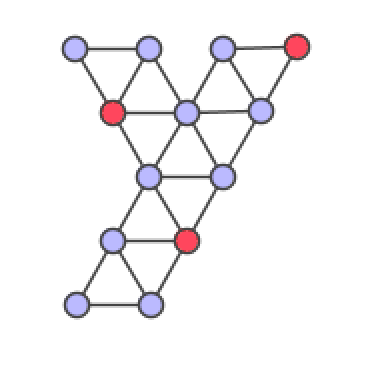
\includegraphics{yagslogo.png}}\par} \end{minipage}

\end{center}\vfill

\mbox{}\\
{\mbox{}\\
\small \noindent \textbf{R. MacKinney-Romero  }  Email: \href{mailto://rene@xanum.uam.mx} {\texttt{rene@xanum.uam.mx}}}\\
{\mbox{}\\
\small \noindent \textbf{M.A. Piza{\~n}a   }  Email: \href{mailto://mpizana@gmail.com} {\texttt{mpizana@gmail.com}}\\
  Homepage: \href{http://xamanek.izt.uam.mx/map/} {\texttt{http://xamanek.izt.uam.mx/map/}}}\\
{\mbox{}\\
\small \noindent \textbf{ R. Villarroel-Flores   }  Email: \href{mailto://rvf0068@gmail.com} {\texttt{rvf0068@gmail.com}}\\
  Homepage: \href{http://rvf0068.github.io} {\texttt{http://rvf0068.github.io}}}\\
\end{titlepage}

\newpage\setcounter{page}{2}
{\small 
\section*{Copyright}
\logpage{[ 0, 0, 2 ]}
 

\textsf{YAGS} - Yet Another Graph System\\
 Copyright {\copyright} 2016 R. MacKinney-Romero, M.A. Piza{\~n}a and R.
Villarroel-Flores. 

This program is free software: you can redistribute it and/or modify it under
the terms of the GNU General Public License as published by the Free Software
Foundation, either version 3 of the License, or (at your option) any later
version. 

This program is distributed in the hope that it will be useful, but WITHOUT
ANY WARRANTY; without even the implied warranty of MERCHANTABILITY or FITNESS
FOR A PARTICULAR PURPOSE. See the GNU General Public License for more details. 

For details, see the file GPL in the installation directory of \textsf{YAGS} typically under \texttt{GAP-DIR/pkg/yags/GPL} or see \href{http://www.gnu.org/licenses/gpl-3.0.html} {\texttt{http://www.gnu.org/licenses/gpl-3.0.html}}. 

\textsc{Contact information:}\\
 M.A. Piza{\~n}a \\
 \href{mailto://yags@xamanek.izt.uam.mx} {\texttt{yags@xamanek.izt.uam.mx}}\\
 \href{mailto://mpizana@gmail.com} {\texttt{mpizana@gmail.com}}\\
  Departamento de Ingenier{\a'\i}a El{\a'e}ctrica\\
 Universidad Aut{\a'o}noma Metropolitana\\
 Av. San Rafael Atlixco 186.\\
 Col. Vicentina, Del. Iztapalapa\\
 Ciudad de M{\a'e}xico 09340 MEXICO.  \mbox{}}\\[1cm]
{\small 
\section*{Acknowledgements}
\logpage{[ 0, 0, 1 ]}
Partially supported by SEP-CONACyT, grant 183210. \\
\\
 We are also grateful for the support of our Universities:\\
 Universidad Aut{\a'o}noma Metropolitana and Universidad Aut{\a'o}noma del
Estado de Hidalgo. \mbox{}}\\[1cm]
\newpage

\def\contentsname{Contents\logpage{[ 0, 0, 3 ]}}

\tableofcontents
\newpage

 
\chapter{\textcolor{Chapter }{Preface}}\label{preface}
\logpage{[ 1, 0, 0 ]}
\hyperdef{L}{X874E1D45845007FE}{}
{
  
\section{\textcolor{Chapter }{Disclaimer}}\label{disclaimer}
\logpage{[ 1, 1, 0 ]}
\hyperdef{L}{X7DE9980D7BA36BD1}{}
{
  

\textsc{This is not an official release yet}, this is a version in development. This particular version, 0.0.1, changes
from one day to another without warning and even without a change in the
version number. Also, the operations and global variables can still change
name or even disappear without warning. No commitment is made at the moment
concerning compatibility of this version of the software with any future
version. 

As of this writing (16/Feb/2016) there are only two trustworthy chapters in
this manual: Appendixes \hyperref[alltopic]{`\textsf{YAGS} Functions by Topic'} and \hyperref[allalpha]{`\textsf{YAGS} Functions Reference'}; also the file \texttt{cheatsheet-yags.pdf} (within directory: \texttt{YAGSDIR/doc/}) may be useful. All other chapters may contain errors, broken links and
misleading information (with higher probability). 

The first official version will be 0.0.2 and is scheduled to be ready this
year (2016), so come back soon. }

 
\section{\textcolor{Chapter }{Welcome to \textsf{YAGS}}}\label{welcometoyags}
\logpage{[ 1, 2, 0 ]}
\hyperdef{L}{X84CD2E0285ABBBC6}{}
{
  

\textsf{YAGS} - \emph{Yet Another Graph System} is a \textsf{GAP} package for dealing with graphs, in the sense of Graph Theory (not bar graphs,
pie charts nor graphs of functions). Our graphs are then, ordered pairs $G=(V,E)$, where $V$ is a finite set of vertices and $E$ is a finite set of edges which are (ordered or unordered) pairs of vertices. 

\textsf{YAGS} was initiated by M.A. Piza{\~n}a in May 2003, and soon incorporated the work
of R. MacKinney-Romero and R. Villarroel-Flores. It sprang from our need of
computing graphs and graph parameters within our research on graph theory and
clique graphs. Consequently, \textsf{YAGS} is well suited for these purposes. 

\textsf{YAGS} is a \textsf{GAP} package and hence its code is interpreted and not compiled (although some
compilation possibilities exist in \textsf{GAP}). Therefore, from the very beginning, it was clear that speed is not our main
goal. Instead, we wanted a very functional, full-featured system; a system
adequate for rapid prototyping of algorithms; and a quick, easy-to-use, way
for testing the rapidly changing working conjectures that are typical of the
research process. 

Over the years, \textsf{YAGS} grew to its present size of more than 200 methods and more than 8 thousands
lines of code. We considered that all this code and effort could (and should)
be useful for other people and then we decided to engaged in the task of tying
up loose ends and writing this manual. 

We would like to mention that we started using \textsf{GRAPE}, and we are grateful with its author, Leonard H. Soicher, for the very useful
system that we used for several years. But at some point we needed some
Object-Oriented features that were not easy to implement in \textsf{GRAPE} and our own subsystem had to follow its own way. If the reader has a profound
need for having groups acting on her/his graphs, then \textsf{GRAPE} may be the best choice. On the other hand, \textsf{YAGS} offers a much wider set of functions (Appendix \ref{allalpha}); a graph-drawing subsystem (\texttt{Draw} (\ref{Draw})); many methods for dealing with graph homomorphism (Chapter \ref{morphismsofgraphs}); an Object-Oriented approach that simplifies the task of working with
several different graph categories (Chapter \ref{graphcategories}); and a generic backtracking subsystem useful to solve many combinatorial
problems easily (Chapter \ref{backtracking}). }

 
\section{\textcolor{Chapter }{Citing \textsf{YAGS}}}\label{citingyags}
\logpage{[ 1, 3, 0 ]}
\hyperdef{L}{X792C907981C4DFE4}{}
{
  

If you publish a result and you used \textsf{YAGS} during your research, please cite us as you would normally do with a research
paper:\\
\\
 R. MacKinney-Romero, M.A. Piza{\~n}a and R. Villarroel-Flores.\\
 \emph{YAGS - Yet Another Graph System, Version 0.0.1} (2016)\\
 \href{http://xamanek.izt.uam.mx/yags/} {\texttt{http://xamanek.izt.uam.mx/yags/}}\\
\\
 \texttt{ @manual\texttt{\symbol{123}}YAGS, author = \texttt{\symbol{123}}R.
MacKinney-Romero and M.A. Piza{\~n}a and R.
Villarroel-Flores\texttt{\symbol{125}}, title = \texttt{\symbol{123}}YAGS -
Yet Another Graph System, Version 0.0.1\texttt{\symbol{125}}, year =
\texttt{\symbol{123}}2016\texttt{\symbol{125}}, note =
\texttt{\symbol{123}}http://xamanek.izt.uam.mx/yags/\texttt{\symbol{125}},
\texttt{\symbol{125}} }\\
\\
 Also, if you install \textsf{YAGS} we will very happy to know about it, so please contribute to increase world's
happiness by sending us a notification to: \href{mailto://yags@xamanek.izt.uam.mx} {\texttt{yags@xamanek.izt.uam.mx}}. }

 
\section{\textcolor{Chapter }{Authors}}\label{authors}
\logpage{[ 1, 4, 0 ]}
\hyperdef{L}{X7B88101D7EE7EB10}{}
{
  

The authors of \textsf{YAGS} in the chronological order of their first contribution are as follows:\\
\\
 M.A. Piza{\~n}a\\
 Departamento de Ingenier{\a'\i}a El{\a'e}ctrica\\
 Universidad Aut{\a'o}noma Metropolitana\\
 \href{mailto://map@xanum.uam.mx} {\texttt{map@xanum.uam.mx}}\\
\\
 R. MacKinney-Romero\\
 Departamento de Ingenier{\a'\i}a El{\a'e}ctrica\\
 Universidad Aut{\a'o}noma Metropolitana\\
 \href{mailto://rene@xanum.uam.mx} {\texttt{rene@xanum.uam.mx}}\\
\\
 R. Villarroel-Flores\\
 Centro de Investigaci{\a'o}n en Matem{\a'a}ticas\\
 Universidad Aut{\a'o}noma del Estado de Hidalgo\\
 \href{mailto://rafaelv@uaeh.edu.mx} {\texttt{rafaelv@uaeh.edu.mx}} }

 
\section{\textcolor{Chapter }{More Information}}\label{moreinformation}
\logpage{[ 1, 5, 0 ]}
\hyperdef{L}{X80298E137C189819}{}
{
  

More information about \textsf{YAGS} can be found on its official web page: \href{http://xamanek.izt.uam.mx/yags/} {\texttt{http://xamanek.izt.uam.mx/yags/}} 

You can receive notifications about \textsf{YAGS} (i.e. new releases, bug fixes, etc.) by subscribing to its email distribution
list: \href{http://xamanek.izt.uam.mx/cgi-bin/mailman/listinfo/yagsnews/} {\texttt{http://xamanek.izt.uam.mx/cgi-bin/mailman/listinfo/yagsnews/}} 

If you are a developer, you may contribute to our project on our public
repository: \href{https://github.com/yags/main/} {\texttt{https://github.com/yags/main/}} 

Comments, support requests, bug reports and installation notifications are
welcome at \href{mailto://yags@xamanek.izt.uam.mx} {\texttt{yags@xamanek.izt.uam.mx}}. }

 }

 
\chapter{\textcolor{Chapter }{Getting Started}}\label{basics}
\logpage{[ 2, 0, 0 ]}
\hyperdef{L}{X7B1863E17896BCE1}{}
{
  
\section{\textcolor{Chapter }{What is \textsf{YAGS}?}}\label{whatisyags}
\logpage{[ 2, 1, 0 ]}
\hyperdef{L}{X83E7553782F04B65}{}
{
  

\textsf{YAGS} - \emph{Yet Another Graph System} is a \textsf{GAP} package for dealing with graphs, in the sense of Graph Theory (not bar graphs,
pie charts nor graphs of functions). Hence our graphs are ordered pairs $G=(V,E)$, where $V$ is a finite set of vertices and $E$ is a finite set of edges which are (ordered or unordered) pairs of vertices. 

\textsf{YAGS} was designed to be useful for research on graphs theory and clique graphs. It
is a very functional, full-featured system; a system adequate for rapid
prototyping of algorithms; and it is a quick, easy-to-use way, for testing the
rapidly changing working conjectures which are typical of the research
process. 

\textsf{YAGS} offers an ample set of functions (Appendix \ref{allalpha}); a graph-drawing subsystem (\texttt{Draw} (\ref{Draw})); many methods for dealing with graph homomorphism (Chapter \ref{morphismsofgraphs}); an Object-Oriented approach that simplifies the task of working with
several different graph categories (Chapter \ref{graphcategories}); and a generic backtracking subsystem useful to solve many combinatorial
problems easily (Chapter \ref{backtracking}). }

 
\section{\textcolor{Chapter }{Installing \textsf{YAGS} for the impatient}}\label{installingyagsnow}
\logpage{[ 2, 2, 0 ]}
\hyperdef{L}{X822644E979EB54CB}{}
{
  
\begin{enumerate}
\item Install \textsf{GAP} following the instructions at \href{http://www.gap-system.org/} {\texttt{http://www.gap-system.org/}}. 
\item Obtain \textsf{YAGS} from its repository \href{https://github.com/yags/main/archive/master.zip} {\texttt{https://github.com/yags/main/archive/master.zip}}.
\item Unpack \textsf{YAGS}: the contents of the zip file should go under \texttt{GAP-DIR/pkg/yags/}.
\item Test \textsf{YAGS} by running \textsf{GAP}, loading \textsf{YAGS} and executing a few basic commands in a terminal: 


\begin{Verbatim}[commandchars=!@|,fontsize=\small,frame=single,label=Example]
  $ gap
     --- some GAP info here ---
  !gapprompt@gap>| !gapinput@RequirePackage("yags");|
     --- some YAGS info here ---
     true
  !gapprompt@gap>| !gapinput@CliqueNumber(Icosahedron);NumberOfCliques(Icosahedron);|
  3
  20
  !gapprompt@gap>| !gapinput@|
\end{Verbatim}

\item  (Optional) Make us happier by sending us a brief installation notification to \href{mailto://yags@xamanek.izt.uam.mx} {\texttt{yags@xamanek.izt.uam.mx}} 
\end{enumerate}
 

Did it work? Congratulations! Otherwise, consider the following
troubleshooting issues: 


\begin{itemize}
\item \textsc{Is }\textsf{GAP}\textsc{ working?}\\
 Make sure it is. Follow carefully \textsf{GAP}'s installation and troubleshooting procedures. 
\item \textsc{Is the installation directory correct?}\\
 The \emph{\textsf{GAP}'s installation directory}, \texttt{GAP-DIR}, \index{GAP-DIR@\texttt{GAP-DIR}} \index{GAP's installation directory@\textsf{GAP}'s installation directory} is typically something like \texttt{/opt/gap4r7/} (in MS Windows it may look like \texttt{C:\texttt{\symbol{92}}gap4r7\texttt{\symbol{92}}}). If this is the case, the \emph{\textsf{YAGS}'s installation directory}, \texttt{YAGS-DIR}, is \index{YAGS-DIR} \index{YAGS's installation directory@\textsf{YAGS}'s installation directory} \texttt{/opt/gap4r7/pkg/yags/} (in Windows, it would be \texttt{C:\texttt{\symbol{92}}gap4r7\texttt{\symbol{92}}pkg\texttt{\symbol{92}}yags\texttt{\symbol{92}}}). Then, the full path for \textsf{YAGS}'s info file \texttt{PackageInfo.g} should be \texttt{/opt/gap4r7/pkg/yags/PackageInfo.g} (or \texttt{C:\texttt{\symbol{92}}gap4r7\texttt{\symbol{92}}pkg\texttt{\symbol{92}}yags\texttt{\symbol{92}}PackageInfo.g}) 
\item \textsc{Are you using }\textsf{GRAPE}\textsc{?}\\
 \textsf{GRAPE} and \textsf{YAGS} are incompatible: they can not be loaded at the same time. If you had an
initialization file that loads \textsf{GRAPE} automatically, you should disable it in order to use \textsf{YAGS}. Alternatively, the command \texttt{gap -r} starts gap diasabling any user-specific configuration files. 
\item \textsc{Unauthorized to access }\textsf{GAP}\textsc{'s directories?}\\
 The installation procedure above assumed that you have full access to your
computer (i.e. that you are the root of the system or that you are using your
PC or Mac). If this is not the case, you can also install \textsf{YAGS} under your user directory. For instance, if your user directory is \texttt{/home/mike/} then you can create a subdirectory \texttt{/home/mike/gaplocal/} and hence your \textsf{YAGS}'s installation directory will be \texttt{/home/mike/gaplocal/pkg/yags/}. If you do this, you can start \textsf{GAP} using \texttt{gap -l ";/home/mike/gaplocal"} so that \textsf{GAP} knows where your \textsf{YAGS} is. 
\end{itemize}
 

Finally, if you are fond of \texttt{git}, then you could clone our repository as usual:\\
 \texttt{git clone http://github.com/yags/main.git GAP-DIR/pkg/yags}. }

 
\section{\textcolor{Chapter }{Installing \textsf{YAGS} with more details}}\label{installingyags}
\logpage{[ 2, 3, 0 ]}
\hyperdef{L}{X7839694378A4C2C1}{}
{
  

If the previous section was too technical for you, here we do the same at a
slower pace. 

First, there are some differences in the installation prodedure depending on
your operating system so we divided this section into several subsections to
cover the most common cases. If your operating system is not covered here, we
do not know yet how to install \textsf{YAGS} on your system, but we welcome your input on the issue. Otherwise just jump
straight to the subsection describing the installation procedure for your
operating system. 
\subsection{\textcolor{Chapter }{Installing \textsf{YAGS} on Windows}}\label{installonwindows}
\logpage{[ 2, 3, 1 ]}
\hyperdef{L}{X7F5295CB7ECEC4FB}{}
{
  

*** installing gap. 

*** installation directory vs working directory. 

*** yags: get, unpack, move. 

*** global versus local installations 

*** yags vs grape clashes. }

 
\subsection{\textcolor{Chapter }{Installing \textsf{YAGS} on Mac OS X}}\label{installonmac}
\logpage{[ 2, 3, 2 ]}
\hyperdef{L}{X822A22A683834A76}{}
{
  

*** installing gap. 

*** installation directory vs working directory. 

*** yags: get, unpack, move. 

*** global versus local installations. 

*** yags vs grape clashes. }

 
\subsection{\textcolor{Chapter }{Installing \textsf{YAGS} on GNU/Linux}}\label{installonunix}
\logpage{[ 2, 3, 3 ]}
\hyperdef{L}{X7FD6343D7B614A4D}{}
{
  

*** installing gap. 

*** installation directory vs working directory. 

*** yags: get, unpack, move. 

*** global versus local installations. 

*** yags vs grape clashes. }

 }

 
\section{\textcolor{Chapter }{A Gentle Tutorial}}\label{agentletutorial}
\logpage{[ 2, 4, 0 ]}
\hyperdef{L}{X875B75517E6E6576}{}
{
  

 This tutorial assumes that you already installed \textsf{GAP} and \textsf{YAGS}; and that you have some basic understanding of \textsf{GAP}: user interface, the read-evaluation loop, aritmetic operations, and lists.
It is strongly recomended that you have some \emph{working directory}, \texttt{WORKING-DIR}, \index{working directory} \index{WORKING-DIR} different from your \textsf{GAP}'s and \textsf{YAGS}'s installation directories. For instance, if your home directory is \texttt{/home/mike/} your working directory could be \texttt{/home/mike/Yags/}. Then you should open a terminal, move to your working directory, start \textsf{GAP} and then, load \textsf{YAGS}: 
\begin{Verbatim}[commandchars=!@|,fontsize=\small,frame=single,label=Example]
  /home/mike> cd Yags
  /home/mike/Yags> gap
     --- some GAP info here ---
  !gapprompt@gap>| !gapinput@RequirePackage("yags");|
     --- some YAGS info here ---
     true
  !gapprompt@gap>| !gapinput@|
\end{Verbatim}
 

The exact appearance of your system prompt (\texttt{/home/mike{\textgreater}} and \texttt{/home/map/Yags/{\textgreater}} in the example) may be different depending on your system, but the commands '\texttt{cd YAGS}' and '\texttt{gap}' are actually the same in all supported systems (assuming your working
directory exists and is named 'Yags'). From there (starting with the command '\texttt{RequirePackage("yags");}') everything happens within \textsf{GAP} and hence it is system-independent. 

Now we want to define some graph. Say we have the list of edges of the desired
graph: 
\[ \{ \{ 1, 2 \}, \{ 2, 3 \}, \{ 3, 4 \}, \{ 4, 1 \}, \{ 1, 5 \}, \{ 5, 4 \} \} \]
 

We can put those edges in a list and then construct the graph: 
\begin{Verbatim}[commandchars=!@|,fontsize=\small,frame=single,label=Example]
  !gapprompt@gap>| !gapinput@list:=[[1,2],[2,3],[3,4],[4,1],[1,5],[5,4]];|
  [ [ 1, 2 ], [ 2, 3 ], [ 3, 4 ], [ 4, 1 ], [ 1, 5 ], [ 5, 4 ] ]
  !gapprompt@gap>| !gapinput@g:=GraphByEdges(list);                      |
  Graph( Category := SimpleGraphs, Order := 5, Size := 
  6, Adjacencies := [ [ 2, 4, 5 ], [ 1, 3 ], [ 2, 4 ], [ 1, 3, 5 ], 
    [ 1, 4 ] ] )  
\end{Verbatim}
 

Note that lists \textsf{GAP} uses brackets ('\texttt{[}' and '\texttt{]}') instead of braces ('\texttt{\texttt{\symbol{123}}}' and '\texttt{\texttt{\symbol{125}}}') to represent sets and lists (actually, in \textsf{GAP} a set is simply an ordered list). Note also that in \textsf{GAP} '\texttt{list}' and '\texttt{List}' are two different things and you can not use the latter since it is a
reserved word of \textsf{GAP}. In general, it is better for you to use lowercase names for your variables,
to avoid name clashes, since all functions in \textsf{GAP} and \textsf{YAGS} start with an uppercase letter. 

The result in the previous example says that it is a graph, and a \emph{simple graph}. By default all graphs in \textsf{YAGS} are simple (no loops, no arrows, no parallel edges, only plain undirected
edges), in Chapter \ref{graphcategories} we explain how to work with other types of graphs, like digraphs, oriented
graphs, and graphs that may have loops (but no parallel edges are suppported
in \textsf{YAGS} at all). In this gentle tutorial all our graphs are simple. 

The result also says, that the just constructed graph \texttt{g} have \texttt{5} vertices and \texttt{6} edges. The reported list of adjacencies means that the vertex \texttt{1} is adjacent (connected by an edge) to \texttt{2}, \texttt{3} and \texttt{4}, that the vertex \texttt{2} is adjacent to \texttt{1} and \texttt{3} and so on. 

To be sure, we can draw our graph and check if it is the intended graph: 
\begin{Verbatim}[commandchars=!@|,fontsize=\small,frame=single,label=Example]
  !gapprompt@gap>| !gapinput@Draw(g);|
\end{Verbatim}
 

A separate window appears with an editable drawing of the graph (but the graph
itself is not editable here). On that window, type: '\texttt{D}' (toggle dynamics on/off), '\texttt{L}' (toggle labels on/off) and '\texttt{F}' (fit graph into window) to obtain a nice drawing (the initial one is
random). The full list of keyboard commands for the \texttt{Draw} window is displayed when typing '\texttt{H}' (toggle help message). Besides these keyboard commands, you can use your
mose in obvious ways to edit the drawing. 

To quit, type '\texttt{S}'. The drawing is stored within the graph \texttt{g} and remembered by \textsf{YAGS} in case you want to draw the graph again. 

As with any command in \textsf{GAP}/\textsf{YAGS}, in case of doubt, you can always access the online help by typing: 
\begin{Verbatim}[commandchars=!@|,fontsize=\small,frame=single,label=Example]
  !gapprompt@gap>| !gapinput@?yags:draw|
  Help: several entries match this topic - type ?2 to get match [2]
  
  [1] yags: Draw
  [2] yags: Drawing
  !gapprompt@gap>| !gapinput@?1|
    B.1-55 Draw
    
    > Draw( G ) --------------------------------------------- operation
    
    Takes a graph G and makes a drawing of it in a separate window. The
    user  can  then  view  and  modify the drawing and finally save the
    vertex coordinates of the drawing into the graph G.
    
    --- many more lines here ---
\end{Verbatim}
 

Here, '\texttt{?}' specifies that we want help; '\texttt{yags:}' specifies on which manual book we want to search (\textsf{YAGS}'s book in this case) and '\texttt{draw}' especifies the topic we would like to be informed about. As it is common,
there are more than one place with information on our topic, hence we choose
among the options with '\texttt{?1}' in the next command line. It is not necessary to specify the book, but then
you could receive many more options, in different books, about some specific
topic. 

Now that we know that our graph is the one we want, we can ask \textsf{YAGS} a lot of things about it: 
\begin{Verbatim}[commandchars=!@|,fontsize=\small,frame=single,label=Example]
  !gapprompt@gap>| !gapinput@Order(g); Size(g); Diameter(g); Girth(g);|
  5
  6
  2
  3
  !gapprompt@gap>| !gapinput@NumberOfCliques(g); CliqueNumber(g);                  |
  4
  3
  !gapprompt@gap>| !gapinput@Adjacencies(g);Adjacency(g,4);Adjacency(g,3);|
  [ [ 2, 4, 5 ], [ 1, 3 ], [ 2, 4 ], [ 1, 3, 5 ], [ 1, 4 ] ]
  [ 1, 3, 5 ]
  [ 2, 4 ]
  !gapprompt@gap>| !gapinput@VertexDegrees(g);VertexDegree(g,4);VertexDegree(g,3);|
  [ 3, 2, 2, 3, 2 ]
  3
  2
  !gapprompt@gap>| !gapinput@IsDiamondFree(g);IsCompleteGraph(g);IsLoopless(g);|
  true
  false
  true
  !gapprompt@gap>| !gapinput@Cliques(g);CompletesOfGivenOrder(g,3);|
  [ [ 1, 4, 5 ], [ 1, 2 ], [ 2, 3 ], [ 3, 4 ] ]
  [ [ 1, 4, 5 ] ]
  !gapprompt@gap>| !gapinput@CompletesOfGivenOrder(g,2);           |
  [ [ 1, 2 ], [ 1, 4 ], [ 1, 5 ], [ 2, 3 ], [ 3, 4 ], [ 4, 5 ] ]
\end{Verbatim}
 

Note that in \textsf{YAGS} a \emph{clique} is always \emph{maximal}. This is just a small sample. There are many more operations, properties and
atributes of graphs already programmed and ready to use. They are all listed
alphabetically in Appendix \ref{allalpha} and by topic in Appendix \ref{alltopic}. There is also a one-page pdf file \texttt{YAGS-DIR/doc/cheatsheet-yags.pdf} which contains a very useful synopsis of many of the most common \textsf{YAGS} operations. 

What about \emph{modifying} our graphs\index{modifying graphs}? Well, all graphs in \textsf{YAGS} are always immutable, which means that, once created, we can never modify a
graph. But we can create new graphs which are variations of existing ones: 
\begin{Verbatim}[commandchars=!@|,fontsize=\small,frame=single,label=Example]
  !gapprompt@gap>| !gapinput@g;|
  Graph( Category := SimpleGraphs, Order := 5, Size := 
  6, Adjacencies := [ [ 2, 4, 5 ], [ 1, 3 ], [ 2, 4 ], [ 1, 3, 5 ], 
    [ 1, 4 ] ] )
  !gapprompt@gap>| !gapinput@h:=AddEdges(g,[[1,3],[2,4]]);;  |
  !gapprompt@gap>| !gapinput@g;|
  Graph( Category := SimpleGraphs, Order := 5, Size := 
  6, Adjacencies := [ [ 2, 4, 5 ], [ 1, 3 ], [ 2, 4 ], [ 1, 3, 5 ], 
    [ 1, 4 ] ] )
  !gapprompt@gap>| !gapinput@h;|
  Graph( Category := SimpleGraphs, Order := 5, Size := 
  8, Adjacencies := [ [ 2, 3, 4, 5 ], [ 1, 3, 4 ], [ 1, 2, 4 ], 
    [ 1, 2, 3, 5 ], [ 1, 4 ] ] )
\end{Verbatim}
 

Note that the graph \texttt{g} remains the same, but the graph \texttt{h} has two additional edges. This is done in this way, because in \textsf{YAGS} everything that is computed about a graph is stored within the graph, so that
we never need to compute something twice. This saves time when computing heavy
attributes of graphs (like computing cliques and clique graphs), but at the
expense of having to make a copy of the graph when we just want a small
variation of it. 

 There are a lot of predefined graphs (the full list can be consulted in
Appendix \ref{tfamilies}): 
\begin{Verbatim}[commandchars=!@|,fontsize=\small,frame=single,label=Example]
  !gapprompt@gap>| !gapinput@PathGraph(5);CycleGraph(6);CompleteGraph(5); |
  Graph( Category := SimpleGraphs, Order := 5, Size := 
  4, Adjacencies := [ [ 2 ], [ 1, 3 ], [ 2, 4 ], [ 3, 5 ], [ 4 ] ] )
  Graph( Category := SimpleGraphs, Order := 6, Size := 
  6, Adjacencies := [ [ 2, 6 ], [ 1, 3 ], [ 2, 4 ], [ 3, 5 ], 
    [ 4, 6 ], [ 1, 5 ] ] )
  Graph( Category := SimpleGraphs, Order := 5, Size := 
  10, Adjacencies := [ [ 2, 3, 4, 5 ], [ 1, 3, 4, 5 ], [ 1, 2, 4, 5 ], 
    [ 1, 2, 3, 5 ], [ 1, 2, 3, 4 ] ] )
  !gapprompt@gap>| !gapinput@CompleteBipartiteGraph(3,3);TreeGraph([2,2,2]);|
  Graph( Category := SimpleGraphs, Order := 6, Size := 
  9, Adjacencies := [ [ 4, 5, 6 ], [ 4, 5, 6 ], [ 4, 5, 6 ], 
    [ 1, 2, 3 ], [ 1, 2, 3 ], [ 1, 2, 3 ] ] )
  Graph( Category := SimpleGraphs, Order := 15, Size := 
  14, Adjacencies := [ [ 2, 3 ], [ 1, 4, 5 ], [ 1, 6, 7 ], 
    [ 2, 8, 9 ], [ 2, 10, 11 ], [ 3, 12, 13 ], [ 3, 14, 15 ], [ 4 ], 
    [ 4 ], [ 5 ], [ 5 ], [ 6 ], [ 6 ], [ 7 ], [ 7 ] ] )
  !gapprompt@gap>| !gapinput@Octahedron;ChairGraph;ParapluieGraph;|
  Graph( Category := SimpleGraphs, Order := 6, Size := 
  12, Adjacencies := [ [ 3, 4, 5, 6 ], [ 3, 4, 5, 6 ], [ 1, 2, 5, 6 ], 
    [ 1, 2, 5, 6 ], [ 1, 2, 3, 4 ], [ 1, 2, 3, 4 ] ] )
  Graph( Category := SimpleGraphs, Order := 5, Size := 
  4, Adjacencies := [ [ 2 ], [ 1, 3, 4 ], [ 2 ], [ 2, 5 ], [ 4 ] ] )
  Graph( Category := SimpleGraphs, Order := 7, Size := 
  9, Adjacencies := [ [ 2 ], [ 1, 3 ], [ 2, 4, 5, 6, 7 ], [ 3, 5 ], 
    [ 3, 4, 6 ], [ 3, 5, 7 ], [ 3, 6 ] ] )
\end{Verbatim}
 

We have found that \texttt{GraphByWalks} (\ref{GraphByWalks}) is one of the most useful and versatile ways of specifying graphs, try to
habituate to it. 
\begin{Verbatim}[commandchars=!@|,fontsize=\small,frame=single,label=Example]
  !gapprompt@gap>| !gapinput@p5:=PathGraph(5);;c6:=CycleGraph(6);;w4:=WheelGraph(4);;  |
  !gapprompt@gap>| !gapinput@IsIsomorphicGraph(p5,GraphByWalks([1..5]));|
  true
  !gapprompt@gap>| !gapinput@IsIsomorphicGraph(c6,GraphByWalks([1,2,3,4,5,6,1]));|
  true
  !gapprompt@gap>| !gapinput@IsIsomorphicGraph(c6,GraphByWalks([1..6],[6,1]));   |
  true
  !gapprompt@gap>| !gapinput@IsIsomorphicGraph(w4,GraphByWalks([1,[2,3,4,5,2]]));|
  true
  !gapprompt@gap>| !gapinput@sd1:=SnubDisphenoid;;                               |
  !gapprompt@gap>| !gapinput@sd2:=GraphByWalks([1,[2,3,4,5],6],[5,[6,7,8,1],2]);; |
  !gapprompt@gap>| !gapinput@IsIsomorphicGraph(sd1,sd2);|
  true
\end{Verbatim}
 }

 
\section{\textcolor{Chapter }{An Overview of the Manual}}\label{anoverviewofthemanual}
\logpage{[ 2, 5, 0 ]}
\hyperdef{L}{X80C41AD78251CB64}{}
{
  }

 
\section{\textcolor{Chapter }{Cheatsheet}}\label{cheatsheet}
\logpage{[ 2, 6, 0 ]}
\hyperdef{L}{X7AC1C7197E9E9112}{}
{
  }

 }

 
\chapter{\textcolor{Chapter }{Cliques}}\label{cliques}
\logpage{[ 3, 0, 0 ]}
\hyperdef{L}{X7AA94AAB7961CEC0}{}
{
  
\section{\textcolor{Chapter }{Cliques and Clique Number}}\label{cliquesandcliquenumber}
\logpage{[ 3, 1, 0 ]}
\hyperdef{L}{X786467B78756F151}{}
{
  }

 
\section{\textcolor{Chapter }{Clique Graphs}}\label{cliquegraphs}
\logpage{[ 3, 2, 0 ]}
\hyperdef{L}{X7EC084CC84A85A76}{}
{
  }

 
\section{\textcolor{Chapter }{Basements, Stars and Neckties}}\label{basementsstarsandneckties}
\logpage{[ 3, 3, 0 ]}
\hyperdef{L}{X7E2DB072791C07A4}{}
{
  }

 
\section{\textcolor{Chapter }{Clique Behavior}}\label{cliquebehavior}
\logpage{[ 3, 4, 0 ]}
\hyperdef{L}{X796DE8297FFED431}{}
{
  }

 }

 
\chapter{\textcolor{Chapter }{Graph Categories}}\label{graphcategories}
\logpage{[ 4, 0, 0 ]}
\hyperdef{L}{X7D6C8738844AF8D4}{}
{
  
\section{\textcolor{Chapter }{The Default Graph Category}}\label{thedefaulgraphcategory}
\logpage{[ 4, 1, 0 ]}
\hyperdef{L}{X814CBBB3834F75F2}{}
{
  }

 
\section{\textcolor{Chapter }{The Target Graph Category}}\label{thetargetgraphcategory}
\logpage{[ 4, 2, 0 ]}
\hyperdef{L}{X7871B6627DE80FF8}{}
{
  }

 
\section{\textcolor{Chapter }{Changing the Target Graph Category Temporaryly}}\label{changingthetargetgraphscategorytemporaly}
\logpage{[ 4, 3, 0 ]}
\hyperdef{L}{X7FCC3B977D58AFEB}{}
{
  }

 
\section{\textcolor{Chapter }{Digraphs, Tournaments, etc.}}\label{digraphstournamentsetc}
\logpage{[ 4, 4, 0 ]}
\hyperdef{L}{X816B21B0866ECFEA}{}
{
  }

 }

 
\chapter{\textcolor{Chapter }{Morphisms of Graphs}}\label{morphismsofgraphs}
\logpage{[ 5, 0, 0 ]}
\hyperdef{L}{X7AB9CE86793A0114}{}
{
  
\section{\textcolor{Chapter }{A Quick Start}}\label{aquickstart}
\logpage{[ 5, 1, 0 ]}
\hyperdef{L}{X815230D9851D5961}{}
{
  }

 
\section{\textcolor{Chapter }{Main Procedures}}\label{mainprocedures}
\logpage{[ 5, 2, 0 ]}
\hyperdef{L}{X825944D279109FDC}{}
{
  }

 
\section{\textcolor{Chapter }{User-Defined Types of Morphisms}}\label{userdefinedtypesofmorphisms}
\logpage{[ 5, 3, 0 ]}
\hyperdef{L}{X7A23DC0E7C318B24}{}
{
  }

 
\section{\textcolor{Chapter }{Predefined Types of Morphisms}}\label{predefinedtypesofmorphisms}
\logpage{[ 5, 4, 0 ]}
\hyperdef{L}{X7C6AE3D882EEFFFF}{}
{
  }

 }

 
\chapter{\textcolor{Chapter }{Backtracking}}\label{backtracking}
\logpage{[ 6, 0, 0 ]}
\hyperdef{L}{X82DE80EC7BC3EF58}{}
{
  
\section{\textcolor{Chapter }{A Simple Example}}\label{asimpleexample}
\logpage{[ 6, 1, 0 ]}
\hyperdef{L}{X7F9B599B7C248828}{}
{
  }

 
\section{\textcolor{Chapter }{How Does it Work?}}\label{howdoesitwork}
\logpage{[ 6, 2, 0 ]}
\hyperdef{L}{X81F0E34D8309D890}{}
{
  }

 
\section{\textcolor{Chapter }{Backtracking in Depth}}\label{backtrackingindepth}
\logpage{[ 6, 3, 0 ]}
\hyperdef{L}{X83019AD37D3C77B6}{}
{
  }

 }

 

\appendix


\chapter{\textcolor{Chapter }{\textsf{YAGS} Functions by Topic}}\label{alltopic}
\logpage{[ "A", 0, 0 ]}
\hyperdef{L}{X80E1CB8A7907178D}{}
{
  A complete list of all \textsf{YAGS}'s functions by topic. 
\section{\textcolor{Chapter }{Most Common Functions}}\label{tmostcommonfunctions}
\logpage{[ "A", 1, 0 ]}
\hyperdef{L}{X7C2382C381CC357C}{}
{
  
\begin{itemize}
\item \texttt{AddEdges( \mbox{\texttt{\mdseries\slshape G}}, \mbox{\texttt{\mdseries\slshape E}} )}\\
 Returns a new graph obtained from \mbox{\texttt{\mdseries\slshape G}} by adding the list of edges in \mbox{\texttt{\mdseries\slshape E}}. (\ref{AddEdges}) 
\item \texttt{Adjacency( \mbox{\texttt{\mdseries\slshape G}}, \mbox{\texttt{\mdseries\slshape x}} )}\\
 Returns the list of vertices in \mbox{\texttt{\mdseries\slshape G}} which are adjacent to vertex \mbox{\texttt{\mdseries\slshape x}}. (\ref{Adjacency}) 
\item \texttt{AutomorphismGroup( \mbox{\texttt{\mdseries\slshape G}} )}\\
 Returns the automorphism group of graph \mbox{\texttt{\mdseries\slshape G}}. A synonym is \texttt{AutGroupGraph( \mbox{\texttt{\mdseries\slshape G}} )}. (\ref{AutomorphismGroup}) 
\item \texttt{BoxProduct( \mbox{\texttt{\mdseries\slshape G}}, \mbox{\texttt{\mdseries\slshape H}} );}\\
 Returns the BoxProduct (or cartesian product) of graphs \mbox{\texttt{\mdseries\slshape G}} and \mbox{\texttt{\mdseries\slshape H}}. (\ref{BoxProduct}) 
\item \texttt{BoxTimesProduct( \mbox{\texttt{\mdseries\slshape G}}, \mbox{\texttt{\mdseries\slshape H}} )}\\
 Returns the BoxTimesProduct (or strong product) of graphs \mbox{\texttt{\mdseries\slshape G}} and \mbox{\texttt{\mdseries\slshape H}}. (\ref{BoxTimesProduct}) 
\item \texttt{Circulant( \mbox{\texttt{\mdseries\slshape n}}, \mbox{\texttt{\mdseries\slshape Jumps}} )}\\
 Returns minimal $(1, 2, ..., n)$-invariant graph where vertex 1 is adjacent to vertices in \mbox{\texttt{\mdseries\slshape Jumps}}. (\ref{Circulant}) 
\item \texttt{CliqueGraph( \mbox{\texttt{\mdseries\slshape G}} )}\\
 \texttt{CliqueGraph( \mbox{\texttt{\mdseries\slshape G}}, \mbox{\texttt{\mdseries\slshape maxNumCli}} )}\\
 Returns the intersection graph of the (maximal) cliques of \mbox{\texttt{\mdseries\slshape G}}; aborts if \mbox{\texttt{\mdseries\slshape maxNumCli}} cliques are found. (\ref{CliqueGraph}) 
\item \texttt{Cliques( \mbox{\texttt{\mdseries\slshape G}} )}\\
 \texttt{Cliques( \mbox{\texttt{\mdseries\slshape G}}, \mbox{\texttt{\mdseries\slshape maxNumCli}} )}\\
 Returns the list of (maximal) cliques of \mbox{\texttt{\mdseries\slshape G}}; aborts if \mbox{\texttt{\mdseries\slshape maxNumCli}} cliques are found. (\ref{Cliques}) 
\item \texttt{ComplementGraph( \mbox{\texttt{\mdseries\slshape G}} )}\\
 Returns the new graph \mbox{\texttt{\mdseries\slshape H}} such that $V(H)=V(G)$ and $xy\in E(H) \iff xy \not\in E(G)$. (\ref{ComplementGraph}) 
\item \texttt{CompleteGraph( \mbox{\texttt{\mdseries\slshape n}} )}\\
 Returns the graph on \mbox{\texttt{\mdseries\slshape n}} vertices having all possible edges present. (\ref{CompleteGraph}) 
\item \texttt{CompleteMultipartiteGraph( \mbox{\texttt{\mdseries\slshape n1}}, \mbox{\texttt{\mdseries\slshape n2}} [, \mbox{\texttt{\mdseries\slshape n3}} ...] )}\\
 Returns the graph with $r\geq 2$ parts of orders \mbox{\texttt{\mdseries\slshape n1}}, \mbox{\texttt{\mdseries\slshape n2}}, ... such that each vertex is adjacent exactly to all the vertices in the
other parts not containing itself. (\ref{CompleteMultipartiteGraph}) 
\item \texttt{ConnectedComponents( \mbox{\texttt{\mdseries\slshape G}} )}\\
 Returns the equivalece partition of $V(G)$ corresponding to the equivalence relation *reachable* in \mbox{\texttt{\mdseries\slshape G}}. (\ref{ConnectedComponents}) 
\item \texttt{CycleGraph( \mbox{\texttt{\mdseries\slshape n}} )}\\
 Returns the cyclic graph on \mbox{\texttt{\mdseries\slshape n}} vertices. (\ref{CycleGraph}) 
\item \texttt{Diameter( \mbox{\texttt{\mdseries\slshape G}} )}\\
 Returns the maximum among the distances between pairs of vertices of \mbox{\texttt{\mdseries\slshape G}}. (\ref{Diameter}) 
\item \texttt{DiscreteGraph( \mbox{\texttt{\mdseries\slshape n}} )}\\
 Returns the graph on \mbox{\texttt{\mdseries\slshape n}} vertices with no edges. (\ref{DiscreteGraph}) 
\item \texttt{DisjointUnion( \mbox{\texttt{\mdseries\slshape G}}, \mbox{\texttt{\mdseries\slshape H}} )}\\
 Returns the disjoint union of two graphs \mbox{\texttt{\mdseries\slshape G}} and \mbox{\texttt{\mdseries\slshape H}}. (\ref{DisjointUnion}) 
\item \texttt{Distance( \mbox{\texttt{\mdseries\slshape G}}, \mbox{\texttt{\mdseries\slshape x}}, \mbox{\texttt{\mdseries\slshape y}} )}\\
 Returns the length of a minimal path connecting \mbox{\texttt{\mdseries\slshape x}} to \mbox{\texttt{\mdseries\slshape y}} in \mbox{\texttt{\mdseries\slshape G}}. (\ref{Distance}) 
\item \texttt{Draw( \mbox{\texttt{\mdseries\slshape G}} )}\\
 Draws the graph \mbox{\texttt{\mdseries\slshape G}} on a new window. (\ref{Draw}) 
\item \texttt{Edges( \mbox{\texttt{\mdseries\slshape G}} )}\\
 Returns the list of edges of graph \mbox{\texttt{\mdseries\slshape G}}. (\ref{Edges}) 
\item \texttt{GraphAttributeStatistics( \mbox{\texttt{\mdseries\slshape OrderList}}, \mbox{\texttt{\mdseries\slshape ProbList}}, \mbox{\texttt{\mdseries\slshape Attribute}} )}\\
 Returns statistics for graph attribute \mbox{\texttt{\mdseries\slshape Attribute}}. (\ref{GraphAttributeStatistics}) 
\item \texttt{GraphByAdjacencies( \mbox{\texttt{\mdseries\slshape AdjList}} )}\\
 Returns a new graph having \mbox{\texttt{\mdseries\slshape AdjList}} as its list of adjacencies. (\ref{GraphByAdjacencies}) 
\item \texttt{GraphByAdjMatrix( \mbox{\texttt{\mdseries\slshape Mat}} )}\\
 Returns a new graph created from an adjacency matrix \mbox{\texttt{\mdseries\slshape Mat}}. (\ref{GraphByAdjMatrix}) 
\item \texttt{GraphByCompleteCover( \mbox{\texttt{\mdseries\slshape Cover}} )}\\
 Returns the graph where the elements of \mbox{\texttt{\mdseries\slshape Cover}} are (the vertex sets of) complete subgraphs. (\ref{GraphByCompleteCover}) 
\item \texttt{GraphByEdges( \mbox{\texttt{\mdseries\slshape L}} )}\\
 Returns the minimal graph such that the pairs in \mbox{\texttt{\mdseries\slshape L}} are edges. (\ref{GraphByEdges}) 
\item \texttt{GraphByRelation( \mbox{\texttt{\mdseries\slshape V}}, \mbox{\texttt{\mdseries\slshape Rel}} )}\\
 \texttt{GraphByRelation( \mbox{\texttt{\mdseries\slshape n}}, \mbox{\texttt{\mdseries\slshape Rel}} )}\\
 Returns a new graph \mbox{\texttt{\mdseries\slshape G}} where $xy \in E(G)$ iff $Rel(x,y)=true$. (\ref{GraphByRelation}) 
\item \texttt{GraphByWalks( \mbox{\texttt{\mdseries\slshape Walk1}}, \mbox{\texttt{\mdseries\slshape Walk2}},...)}\\
 Returns the minimal graph such that \mbox{\texttt{\mdseries\slshape Walk1}}, \mbox{\texttt{\mdseries\slshape Walk2}}, etc are Walks. (\ref{GraphByWalks}) 
\item \texttt{GraphSum( \mbox{\texttt{\mdseries\slshape G}}, \mbox{\texttt{\mdseries\slshape L}} )}\\
 Returns the lexicographic sum of a list of graphs \mbox{\texttt{\mdseries\slshape L}} over a graph \mbox{\texttt{\mdseries\slshape G}}. (\ref{GraphSum}) 
\item \texttt{InducedSubgraph( \mbox{\texttt{\mdseries\slshape G}}, \mbox{\texttt{\mdseries\slshape V}} )}\\
 Returns the subgraph of graph \mbox{\texttt{\mdseries\slshape G}} induced by the vertex set \mbox{\texttt{\mdseries\slshape V}}. (\ref{InducedSubgraph}) 
\item \texttt{InNeigh( \mbox{\texttt{\mdseries\slshape G}}, \mbox{\texttt{\mdseries\slshape x}} )}\\
 Returns the list of in-neighbors of \mbox{\texttt{\mdseries\slshape x}} in \mbox{\texttt{\mdseries\slshape G}}. (\ref{InNeigh}) 
\item \texttt{IntersectionGraph( \mbox{\texttt{\mdseries\slshape L}} )}\\
 Returns the graph \mbox{\texttt{\mdseries\slshape G}} where $V(G)=L$ and $XY\in E(G) \iff X\cap Y \neq \varnothing$. (\ref{IntersectionGraph}) 
\item \texttt{IsEdge( \mbox{\texttt{\mdseries\slshape G}}, \mbox{\texttt{\mdseries\slshape x}}, \mbox{\texttt{\mdseries\slshape y}} )}\\
 \texttt{IsEdge( \mbox{\texttt{\mdseries\slshape G}}, [\mbox{\texttt{\mdseries\slshape x}},\mbox{\texttt{\mdseries\slshape y}}] )}\\
 Returns \texttt{true} if \texttt{[\mbox{\texttt{\mdseries\slshape x}},\mbox{\texttt{\mdseries\slshape y}}]} is an edge of \mbox{\texttt{\mdseries\slshape G}}. (\ref{IsEdge}) 
\item \texttt{IsIsomorphicGraph( \mbox{\texttt{\mdseries\slshape G}}, \mbox{\texttt{\mdseries\slshape H}} )}\\
 Returns \texttt{true} when \mbox{\texttt{\mdseries\slshape G}} is isomorphic to \mbox{\texttt{\mdseries\slshape H}} and \texttt{false} otherwise. (\ref{IsIsomorphicGraph}) 
\item \texttt{Join( \mbox{\texttt{\mdseries\slshape G}}, \mbox{\texttt{\mdseries\slshape H}} )}\\
 Returns the disjoint union of \mbox{\texttt{\mdseries\slshape G}} and \mbox{\texttt{\mdseries\slshape H}} with all the possible edges between \mbox{\texttt{\mdseries\slshape G}} and \mbox{\texttt{\mdseries\slshape H}} added. (\ref{Join}) 
\item \texttt{LineGraph( \mbox{\texttt{\mdseries\slshape G}} )}\\
 Returns the intersection graph of the edges of \mbox{\texttt{\mdseries\slshape G}}. (\ref{LineGraph}) 
\item \texttt{Link( \mbox{\texttt{\mdseries\slshape G}}, \mbox{\texttt{\mdseries\slshape x}} )}\\
 Returns the subgraph induced in \mbox{\texttt{\mdseries\slshape G}} by the neighbors of \mbox{\texttt{\mdseries\slshape x}}. (\ref{Link}) 
\item \texttt{MaxDegree( \mbox{\texttt{\mdseries\slshape G}} )}\\
 Returns the maximum degree in graph \mbox{\texttt{\mdseries\slshape G}}. (\ref{MaxDegree}) 
\item \texttt{Order( \mbox{\texttt{\mdseries\slshape G}} )}\\
 Returns the number of vertices, of graph \mbox{\texttt{\mdseries\slshape G}}. (\ref{Order}) 
\item \texttt{PathGraph( \mbox{\texttt{\mdseries\slshape n}} )}\\
 Returns the path graph on \mbox{\texttt{\mdseries\slshape n}} vertices. (\ref{PathGraph}) 
\item \texttt{QuotientGraph( \mbox{\texttt{\mdseries\slshape G}}, \mbox{\texttt{\mdseries\slshape Part}} )}\\
 \texttt{QuotientGraph( \mbox{\texttt{\mdseries\slshape G}}, \mbox{\texttt{\mdseries\slshape L1}}, \mbox{\texttt{\mdseries\slshape L2}} )}\\
 Returns the quotient graph of graph \mbox{\texttt{\mdseries\slshape G}} given a vertex partition \mbox{\texttt{\mdseries\slshape Part}}, by identifying any two vertices in the same part. (\ref{QuotientGraph}) 
\item \texttt{RandomGraph( \mbox{\texttt{\mdseries\slshape n}}, \mbox{\texttt{\mdseries\slshape p}} )}\\
 \texttt{RandomGraph( \mbox{\texttt{\mdseries\slshape n}} )}\\
 Returns a random graph of order \mbox{\texttt{\mdseries\slshape n}} with edge probability $p$ (a rational in $[0,1]$). (\ref{RandomGraph}) 
\item \texttt{RemoveEdges( \mbox{\texttt{\mdseries\slshape G}}, \mbox{\texttt{\mdseries\slshape E}} )}\\
 Returns a new graph created from graph \mbox{\texttt{\mdseries\slshape G}} by removing the edges in list \mbox{\texttt{\mdseries\slshape E}}. (\ref{RemoveEdges}) 
\item \texttt{SetDefaultGraphCategory( \mbox{\texttt{\mdseries\slshape Catgy}} )}\\
 Sets the default graph category to \mbox{\texttt{\mdseries\slshape Catgy}}. (\ref{SetDefaultGraphCategory}) 
\item \texttt{Size( \mbox{\texttt{\mdseries\slshape G}} )}\\
 Returns the number of edges of graph \mbox{\texttt{\mdseries\slshape G}}. (\ref{Size}) 
\item \texttt{TimesProduct( \mbox{\texttt{\mdseries\slshape G}}, \mbox{\texttt{\mdseries\slshape H}} )}\\
 Returns the times product (tensor product) $G \times H$ of two graphs \mbox{\texttt{\mdseries\slshape G}} and \mbox{\texttt{\mdseries\slshape H}}. (\ref{TimesProduct}) 
\item \texttt{TrivialGraph}\\
 The one vertex graph.(\ref{TrivialGraph}) 
\item \texttt{VertexDegree( \mbox{\texttt{\mdseries\slshape G}}, \mbox{\texttt{\mdseries\slshape x}} )}\\
 Returns the degree of vertex \mbox{\texttt{\mdseries\slshape x}} in Graph \mbox{\texttt{\mdseries\slshape G}}. (\ref{VertexDegree}) 
\item \texttt{VertexNames( \mbox{\texttt{\mdseries\slshape G}} )}\\
 Returns the list of names of the vertices of \mbox{\texttt{\mdseries\slshape G}}. (\ref{VertexNames}) 
\item \texttt{WheelGraph( \mbox{\texttt{\mdseries\slshape n}} )}\\
 \texttt{WheelGraph( \mbox{\texttt{\mdseries\slshape n}}, \mbox{\texttt{\mdseries\slshape r}} )}\\
 This is the cone of an \mbox{\texttt{\mdseries\slshape n}}-cycle; when present, \mbox{\texttt{\mdseries\slshape r}} is the radius of the wheel. (\ref{WheelGraph}) 
\end{itemize}
 }

 
\section{\textcolor{Chapter }{Drawing}}\label{tdrawing}
\logpage{[ "A", 2, 0 ]}
\hyperdef{L}{X7AFE6B467AB077A8}{}
{
  
\begin{itemize}
\item \texttt{Coordinates( \mbox{\texttt{\mdseries\slshape G}} )}\\
 Returns the list of coordinates of the vertices of \mbox{\texttt{\mdseries\slshape G}} if they exist; fail otherwise. (\ref{Coordinates}) 
\item \texttt{Draw( \mbox{\texttt{\mdseries\slshape G}} )}\\
 Draws the graph \mbox{\texttt{\mdseries\slshape G}} on a new window. (\ref{Draw}) 
\item \texttt{GraphToRaw( \mbox{\texttt{\mdseries\slshape FileName}}, \mbox{\texttt{\mdseries\slshape G}} )}\\
 Writes the graph \mbox{\texttt{\mdseries\slshape G}} in raw format to the file \mbox{\texttt{\mdseries\slshape FileName}}. (\ref{GraphToRaw}) 
\item \texttt{GraphUpdateFromRaw( \mbox{\texttt{\mdseries\slshape FileName}}, \mbox{\texttt{\mdseries\slshape G}} )}\\
 Updates the coordinates of \mbox{\texttt{\mdseries\slshape G}} from a file \mbox{\texttt{\mdseries\slshape FileName}} in raw format. (\ref{GraphUpdateFromRaw}) 
\item \texttt{SetCoordinates( \mbox{\texttt{\mdseries\slshape G}}, \mbox{\texttt{\mdseries\slshape Coord}} ) }\\
 Sets the coordinates of the vertices of \mbox{\texttt{\mdseries\slshape G}}, which are used to draw \mbox{\texttt{\mdseries\slshape G}} by \texttt{Draw( \mbox{\texttt{\mdseries\slshape G}} )}. (\ref{SetCoordinates}) 
\end{itemize}
 }

 
\section{\textcolor{Chapter }{Constructing Graphs}}\label{tconstructinggraphs}
\logpage{[ "A", 3, 0 ]}
\hyperdef{L}{X865ECABF7952FB46}{}
{
  
\begin{itemize}
\item \texttt{AddEdges( \mbox{\texttt{\mdseries\slshape G}}, \mbox{\texttt{\mdseries\slshape E}} )}\\
 Returns a new graph obtained from \mbox{\texttt{\mdseries\slshape G}} by adding the list of edges in \mbox{\texttt{\mdseries\slshape E}}. (\ref{AddEdges}) 
\item \texttt{AddVerticesByAdjacencies( \mbox{\texttt{\mdseries\slshape G}}, \mbox{\texttt{\mdseries\slshape NewAdjList}} )}\\
 Returns a new graph obtained from \mbox{\texttt{\mdseries\slshape G}} by adding some vertices with adjacencies described by \mbox{\texttt{\mdseries\slshape NewAdjList}}. (\ref{AddVerticesByAdjacencies}) 
\item \texttt{Graph( \mbox{\texttt{\mdseries\slshape Rec}} )}\\
 Returns a new graph created from the information in record \mbox{\texttt{\mdseries\slshape Rec}}. (\ref{Graph}) 
\item \texttt{GraphByAdjacencies( \mbox{\texttt{\mdseries\slshape AdjList}} )}\\
 Returns a new graph having \mbox{\texttt{\mdseries\slshape AdjList}} as its list of adjacencies. (\ref{GraphByAdjacencies}) 
\item \texttt{GraphByAdjMatrix( \mbox{\texttt{\mdseries\slshape Mat}} )}\\
 Returns a new graph created from an adjacency matrix \mbox{\texttt{\mdseries\slshape Mat}}. (\ref{GraphByAdjMatrix}) 
\item \texttt{GraphByCompleteCover( \mbox{\texttt{\mdseries\slshape Cover}} )}\\
 Returns the graph where the elements of \mbox{\texttt{\mdseries\slshape Cover}} are (the vertex sets of) complete subgraphs. (\ref{GraphByCompleteCover}) 
\item \texttt{GraphByEdges( \mbox{\texttt{\mdseries\slshape L}} )}\\
 Returns the minimal graph such that the pairs in \mbox{\texttt{\mdseries\slshape L}} are edges. (\ref{GraphByEdges}) 
\item \texttt{GraphByRelation( \mbox{\texttt{\mdseries\slshape V}}, \mbox{\texttt{\mdseries\slshape Rel}} )}\\
 \texttt{GraphByRelation( \mbox{\texttt{\mdseries\slshape n}}, \mbox{\texttt{\mdseries\slshape Rel}} )}\\
 Returns a new graph \mbox{\texttt{\mdseries\slshape G}} where $xy \in E(G)$ iff $Rel(x,y)=true$. (\ref{GraphByRelation}) 
\item \texttt{GraphByWalks( \mbox{\texttt{\mdseries\slshape Walk1}}, \mbox{\texttt{\mdseries\slshape Walk2}},...)}\\
 Returns the minimal graph such that \mbox{\texttt{\mdseries\slshape Walk1}}, \mbox{\texttt{\mdseries\slshape Walk2}}, etc are Walks. (\ref{GraphByWalks}) 
\item \texttt{IntersectionGraph( \mbox{\texttt{\mdseries\slshape L}} )}\\
 Returns the graph \mbox{\texttt{\mdseries\slshape G}} where $V(G)=L$ and $XY\in E(G) \iff X\cap Y \neq \varnothing$. (\ref{IntersectionGraph}) 
\item \texttt{RandomGraph( \mbox{\texttt{\mdseries\slshape n}}, \mbox{\texttt{\mdseries\slshape p}} )}\\
 \texttt{RandomGraph( \mbox{\texttt{\mdseries\slshape n}} )}\\
 Returns a random graph of order \mbox{\texttt{\mdseries\slshape n}} with edge probability $p$ (a rational in $[0,1]$). (\ref{RandomGraph}) 
\item \texttt{RemoveEdges( \mbox{\texttt{\mdseries\slshape G}}, \mbox{\texttt{\mdseries\slshape E}} )}\\
 Returns a new graph created from graph \mbox{\texttt{\mdseries\slshape G}} by removing the edges in list \mbox{\texttt{\mdseries\slshape E}}. (\ref{RemoveEdges}) 
\item \texttt{RemoveVertices( \mbox{\texttt{\mdseries\slshape G}}, \mbox{\texttt{\mdseries\slshape V}} )}\\
 Returns a new graph created from graph \mbox{\texttt{\mdseries\slshape G}} by removing the vertices in list \mbox{\texttt{\mdseries\slshape V}}. (\ref{RemoveVertices}) 
\end{itemize}
 }

 
\section{\textcolor{Chapter }{Families of Graphs}}\label{tfamilies}
\logpage{[ "A", 4, 0 ]}
\hyperdef{L}{X82B05AAB844DD947}{}
{
  
\begin{itemize}
\item \texttt{AGraph}\\
 A 4-cycle with two pendant vertices on consecutive vertices of the cycle. (\ref{AGraph}) 
\item \texttt{AntennaGraph}\\
 A \texttt{HouseGraph} with a pendant vertex (antenna) on the roof. (\ref{AntennaGraph}) 
\item \texttt{BullGraph}\\
 A triangle with two pendant vertices (horns). (\ref{BullGraph}) 
\item \texttt{ChairGraph}\\
 A tree with degree sequence 3,2,1,1,1. (\ref{ChairGraph}) 
\item \texttt{Circulant( \mbox{\texttt{\mdseries\slshape n}}, \mbox{\texttt{\mdseries\slshape Jumps}} )}\\
 Returns minimal $(1, 2, ..., n)$-invariant graph where vertex 1 is adjacent to vertices in \mbox{\texttt{\mdseries\slshape Jumps}}. (\ref{Circulant}) 
\item \texttt{ClawGraph}\\
 The graph on 4 vertices, 3 edges, and maximum degree 3. (\ref{ClawGraph}) 
\item \texttt{ClockworkGraph( \mbox{\texttt{\mdseries\slshape NNFSList}} )}\\
 \texttt{ClockworkGraph( \mbox{\texttt{\mdseries\slshape NNFSList}}, \mbox{\texttt{\mdseries\slshape rank}} )}\\
 \texttt{ClockworkGraph( \mbox{\texttt{\mdseries\slshape NNFSList}}, \mbox{\texttt{\mdseries\slshape Perm}} )}\\
 \texttt{ClockworkGraph( \mbox{\texttt{\mdseries\slshape NNFSList}}, \mbox{\texttt{\mdseries\slshape rank}}, \mbox{\texttt{\mdseries\slshape Perm}} )}\\
 Returns the clockwork graph specified by its parameters. (\ref{ClockworkGraph}) 
\item \texttt{CompleteBipartiteGraph( \mbox{\texttt{\mdseries\slshape n}}, \mbox{\texttt{\mdseries\slshape m}} )}\\
 Returns the minimal graph such that all vertices in $\{1..n\}$ are adjacent to all in $\{n+1..n+m\}$. (\ref{CompleteBipartiteGraph}) 
\item \texttt{CompleteGraph( \mbox{\texttt{\mdseries\slshape n}} )}\\
 Returns the graph on \mbox{\texttt{\mdseries\slshape n}} vertices having all possible edges present. (\ref{CompleteGraph}) 
\item \texttt{CompleteMultipartiteGraph( \mbox{\texttt{\mdseries\slshape n1}}, \mbox{\texttt{\mdseries\slshape n2}} [, \mbox{\texttt{\mdseries\slshape n3}} ...] )}\\
 Returns the graph with $r\geq 2$ parts of orders \mbox{\texttt{\mdseries\slshape n1}}, \mbox{\texttt{\mdseries\slshape n2}}, ... such that each vertex is adjacent exactly to all the vertices in the
other parts not containing itself. (\ref{CompleteMultipartiteGraph}) 
\item \texttt{Cube}\\
 The 1-skeleton of Plato's cube. (\ref{Cube}) 
\item \texttt{CubeGraph( \mbox{\texttt{\mdseries\slshape n}} )}\\
 Returns the underlying graph of the \mbox{\texttt{\mdseries\slshape n}}-hypercube. (\ref{CubeGraph}) 
\item \texttt{CycleGraph( \mbox{\texttt{\mdseries\slshape n}} )}\\
 Returns the cyclic graph on \mbox{\texttt{\mdseries\slshape n}} vertices. (\ref{CycleGraph}) 
\item \texttt{CylinderGraph( \mbox{\texttt{\mdseries\slshape b}}, \mbox{\texttt{\mdseries\slshape h}} )}\\
 Returns graph on $b(h+1)$ vertices which is a $\{4,6\}$-regular triangulation of the cylinder. (\ref{CylinderGraph}) 
\item \texttt{DartGraph}\\
 A diamond with a pendant vertex and maximum degree 4. (\ref{DartGraph}) 
\item \texttt{DiamondGraph}\\
 The graph on 4 vertices and 5 edges. (\ref{DiamondGraph}) 
\item \texttt{DiscreteGraph( \mbox{\texttt{\mdseries\slshape n}} )}\\
 Returns the graph on \mbox{\texttt{\mdseries\slshape n}} vertices with no edges. (\ref{DiscreteGraph}) 
\item \texttt{Dodecahedron}\\
 The 1-skeleton of Plato's Dodecahedron. (\ref{Dodecahedron}) 
\item \texttt{DominoGraph}\\
 Two squares glued by an edge. (\ref{DominoGraph}) 
\item \texttt{FanGraph( \mbox{\texttt{\mdseries\slshape n}} )}\\
 Returns the \mbox{\texttt{\mdseries\slshape n}}-Fan: The join of a vertex and a (\mbox{\texttt{\mdseries\slshape n}}+1)-path. (\ref{FanGraph}) 
\item \texttt{FishGraph}\\
 A square and a triangle glued by a vertex. (\ref{FishGraph}) 
\item \texttt{GemGraph}\\
 The 3-Fan graph. (\ref{GemGraph}) 
\item \texttt{HouseGraph}\\
 A 4-Cycle and a triangle glued by an edge. (\ref{HouseGraph}) 
\item \texttt{Icosahedron}\\
 The 1-skeleton of Plato's icosahedron. (\ref{Icosahedron}) 
\item \texttt{JohnsonGraph( \mbox{\texttt{\mdseries\slshape n}}, \mbox{\texttt{\mdseries\slshape r}} )}\\
 Returns a new graph \mbox{\texttt{\mdseries\slshape G}} where $V(G)$ is the set of \mbox{\texttt{\mdseries\slshape r}}-subsets of $\{1,2 \ldots n\}$, two of them being adjacent iff their intersection contains exactly \mbox{\texttt{\mdseries\slshape r}}-1 elements. (\ref{JohnsonGraph}) 
\item \texttt{KiteGraph}\\
 A diamond with a pendant vertex and maximum degree 3. (\ref{KiteGraph}) 
\item \texttt{OctahedralGraph( \mbox{\texttt{\mdseries\slshape n}} )}\\
 Returns the $(2n-2)$-regular graph on $2n$ vertices. (\ref{OctahedralGraph}) 
\item \texttt{Octahedron}\\
 The 1-skeleton of Plato's octahedron. (\ref{Octahedron}) 
\item \texttt{ParachuteGraph}\\
 Returns the suspension of a 4-path with a pendant vertex attached to the south
pole. (\ref{ParachuteGraph}) 
\item \texttt{ParapluieGraph}\\
 A 3-Fan graph with a 3-path attached to the universal vertex. (\ref{ParapluieGraph}) 
\item \texttt{PathGraph( \mbox{\texttt{\mdseries\slshape n}} )}\\
 Returns the path graph on \mbox{\texttt{\mdseries\slshape n}} vertices. (\ref{PathGraph}) 
\item \texttt{PawGraph}\\
 A triangle with a pendant vertex. (\ref{PawGraph}) 
\item \texttt{PetersenGraph}\\
 The 3-regular graph on 10 vertices having girth 5. (\ref{PetersenGraph}) 
\item \texttt{RandomCirculant( \mbox{\texttt{\mdseries\slshape n}} )}\\
 \texttt{RandomCirculant( \mbox{\texttt{\mdseries\slshape n}}, \mbox{\texttt{\mdseries\slshape k}} )}\\
 \texttt{RandomCirculant( \mbox{\texttt{\mdseries\slshape n}}, \mbox{\texttt{\mdseries\slshape p}} )}\\
 Returns a circulant on \mbox{\texttt{\mdseries\slshape n}} vertices with its \mbox{\texttt{\mdseries\slshape jumps}} selected randomly. (\ref{RandomCirculant}) 
\item \texttt{RGraph}\\
 A square with two pendant vertices attached to the same vertex of the square.
(\ref{RGraph}) 
\item \texttt{SnubDisphenoid}\\
 The 1-skeleton of the 84th Johnson solid. (\ref{SnubDisphenoid}) 
\item \texttt{SpikyGraph( \mbox{\texttt{\mdseries\slshape n}} )}\\
 Returns a complete on \mbox{\texttt{\mdseries\slshape n}} vertices, with an additional complete on \mbox{\texttt{\mdseries\slshape n}} vertices glued to each of its (\mbox{\texttt{\mdseries\slshape n}}-1)-dimensional faces. (\ref{SpikyGraph}) 
\item \texttt{SunGraph( \mbox{\texttt{\mdseries\slshape n}} )}\\
 Returns a complete graph on \mbox{\texttt{\mdseries\slshape n}} vertices with a zigzaging corona of 2\mbox{\texttt{\mdseries\slshape n}} vertices glued to a \mbox{\texttt{\mdseries\slshape n}}-cycle of the complete graph. (\ref{SunGraph}) 
\item \texttt{Tetrahedron}\\
 The 1-skeleton of Plato's tetrahedron. (\ref{Tetrahedron}) 
\item \texttt{TorusGraph( \mbox{\texttt{\mdseries\slshape n}}, \mbox{\texttt{\mdseries\slshape m}} )}\\
 Returns (the underlying graph of) a triangulation of the torus on $n.m$ vertices. (\ref{TorusGraph}) 
\item \texttt{TreeGraph( \mbox{\texttt{\mdseries\slshape arity}}, \mbox{\texttt{\mdseries\slshape depth}} )}\\
 \texttt{TreeGraph( \mbox{\texttt{\mdseries\slshape ArityList}} )}\\
 Returns the tree, the connected cycle-free graph, specified by it parameters.
(\ref{TreeGraph}) 
\item \texttt{TrivialGraph}\\
 The one vertex graph. (\ref{TrivialGraph}) 
\item \texttt{WheelGraph( \mbox{\texttt{\mdseries\slshape n}} )}\\
 \texttt{WheelGraph( \mbox{\texttt{\mdseries\slshape n}}, \mbox{\texttt{\mdseries\slshape r}} )}\\
 This is the cone of an \mbox{\texttt{\mdseries\slshape n}}-cycle; when present \mbox{\texttt{\mdseries\slshape r}} is the radius of the wheel. (\ref{WheelGraph}) 
\end{itemize}
 }

 
\section{\textcolor{Chapter }{Small Graphs}}\label{tsmallgraphs}
\logpage{[ "A", 5, 0 ]}
\hyperdef{L}{X870DC04278F413BE}{}
{
  
\begin{itemize}
\item \texttt{ConnectedGraphsOfGivenOrder( \mbox{\texttt{\mdseries\slshape n}} )}\\
 Returns the list of all connected graphs of order \mbox{\texttt{\mdseries\slshape n}} (upto isomorphism). (\ref{ConnectedGraphsOfGivenOrder}) 
\item \texttt{Graph6ToGraph( \mbox{\texttt{\mdseries\slshape String}} )}\\
 Returns the graph represented by \mbox{\texttt{\mdseries\slshape String}} which is encoded using Brendan McKay's graph6 format. (\ref{Graph6ToGraph}) 
\item \texttt{GraphsOfGivenOrder( \mbox{\texttt{\mdseries\slshape n}} )}\\
 Returns the list of all graphs of order \mbox{\texttt{\mdseries\slshape n}} (upto isomorphism). (\ref{GraphsOfGivenOrder}) 
\item \texttt{ImportGraph6( \mbox{\texttt{\mdseries\slshape Filename}} )}\\
 Returns the list of graphs represented in \mbox{\texttt{\mdseries\slshape Filename}} which are encoded using Brendan McKay's graph6 format. (\ref{ImportGraph6}) 
\item \texttt{HararyToMcKay( \mbox{\texttt{\mdseries\slshape Spec}} )}\\
 Returns the McKay's \mbox{\texttt{\mdseries\slshape index}} of a Harary's graph specification \mbox{\texttt{\mdseries\slshape Spec}}. (\ref{HararyToMcKay}) 
\item \texttt{McKayToHarary( \mbox{\texttt{\mdseries\slshape index}} )}\\
 Returns the Harary's graph specification of a McKay's \mbox{\texttt{\mdseries\slshape index}}. (\ref{McKayToHarary}) 
\end{itemize}
 }

 
\section{\textcolor{Chapter }{Attributes and Properties}}\label{tattributesandproperties}
\logpage{[ "A", 6, 0 ]}
\hyperdef{L}{X7DC480E57D26429A}{}
{
  
\begin{itemize}
\item \texttt{Adjacencies( \mbox{\texttt{\mdseries\slshape G}} )}\\
 Returns the list of adjacencies of \mbox{\texttt{\mdseries\slshape G}}: The neighbors of vertex \mbox{\texttt{\mdseries\slshape x}} are listed in position \mbox{\texttt{\mdseries\slshape x}} of that list. (\ref{Adjacencies}) 
\item \texttt{Adjacency( \mbox{\texttt{\mdseries\slshape G}}, \mbox{\texttt{\mdseries\slshape x}} )}\\
 Returns the list of vertices in \mbox{\texttt{\mdseries\slshape G}} which are adjacent to vertex \mbox{\texttt{\mdseries\slshape x}}. (\ref{Adjacency}) 
\item \texttt{AdjMatrix( \mbox{\texttt{\mdseries\slshape G}} )}\\
 Returns the Adjacency Matrix of \mbox{\texttt{\mdseries\slshape G}}. (\ref{AdjMatrix}) 
\item \texttt{AutomorphismGroup( \mbox{\texttt{\mdseries\slshape G}} )}\\
 Returns the automorphism group of graph \mbox{\texttt{\mdseries\slshape G}}. A synonym is \texttt{AutGroupGraph( \mbox{\texttt{\mdseries\slshape G}} )}. (\ref{AutomorphismGroup}) 
\item \texttt{BoundaryVertices( \mbox{\texttt{\mdseries\slshape G}} )}\\
 Returns the list of vertices of \mbox{\texttt{\mdseries\slshape G}} that have links isomorphic to a path. But it returns \texttt{fail} if \mbox{\texttt{\mdseries\slshape G}} is not a compact surface. (\ref{BoundaryVertices}) 
\item \texttt{ConnectedComponents( \mbox{\texttt{\mdseries\slshape G}} )}\\
 Returns the equivalece partition of $V(G)$ corresponding to the equivalence relation \emph{reachable} in \mbox{\texttt{\mdseries\slshape G}}. (\ref{ConnectedComponents}) 
\item \texttt{Diameter( \mbox{\texttt{\mdseries\slshape G}} )}\\
 Returns the maximum among the distances between pairs of vertices of \mbox{\texttt{\mdseries\slshape G}}. (\ref{Diameter}) 
\item \texttt{Distance( \mbox{\texttt{\mdseries\slshape G}}, \mbox{\texttt{\mdseries\slshape x}}, \mbox{\texttt{\mdseries\slshape y}} )}\\
 Returns the length of a minimal path connecting \mbox{\texttt{\mdseries\slshape x}} to \mbox{\texttt{\mdseries\slshape y}} in \mbox{\texttt{\mdseries\slshape G}}. (\ref{Distance}) 
\item \texttt{DistanceMatrix( \mbox{\texttt{\mdseries\slshape G}} )}\\
 Returns an $n\times n$ matrix $D$, where $D[x][y]$ is the distance between \mbox{\texttt{\mdseries\slshape x}} and \mbox{\texttt{\mdseries\slshape y}} in \mbox{\texttt{\mdseries\slshape G}}. (\ref{DistanceMatrix}) 
\item \texttt{DistanceSet( \mbox{\texttt{\mdseries\slshape G}}, \mbox{\texttt{\mdseries\slshape A}}, \mbox{\texttt{\mdseries\slshape B}} )}\\
 Returns the set of distances between pairs of vertices in $A\times B$. (\ref{DistanceSet}) 
\item \texttt{Distances( \mbox{\texttt{\mdseries\slshape G}}, \mbox{\texttt{\mdseries\slshape A}}, \mbox{\texttt{\mdseries\slshape B}} )}\\
 Returns the list of distances between pairs of vertices in $A\times B$. (\ref{Distances}) 
\item \texttt{DominatedVertices( \mbox{\texttt{\mdseries\slshape G}} )}\\
 Returns the set of dominated vertices of \mbox{\texttt{\mdseries\slshape G}}. (\ref{DominatedVertices}) 
\item \texttt{Eccentricity( \mbox{\texttt{\mdseries\slshape G}}, \mbox{\texttt{\mdseries\slshape x}} )}\\
 Returns the distance from a vertex \mbox{\texttt{\mdseries\slshape x}} in graph \mbox{\texttt{\mdseries\slshape G}} to its most distant vertex in \mbox{\texttt{\mdseries\slshape G}}. (\ref{Eccentricity}) 
\item \texttt{Edges( \mbox{\texttt{\mdseries\slshape G}} )}\\
 Returns the list of edges of graph \mbox{\texttt{\mdseries\slshape G}}. (\ref{Edges}) 
\item \texttt{Girth( \mbox{\texttt{\mdseries\slshape G}} )}\\
 Returns the length of the minimum induced cycle in \mbox{\texttt{\mdseries\slshape G}}. (\ref{Girth}) 
\item \texttt{GraphAttributeStatistics( \mbox{\texttt{\mdseries\slshape OrderList}}, \mbox{\texttt{\mdseries\slshape ProbList}}, \mbox{\texttt{\mdseries\slshape Attribute}} )}\\
 Returns statistics for graph attribute \mbox{\texttt{\mdseries\slshape Attribute}}. (\ref{GraphAttributeStatistics}) 
\item \texttt{InteriorVertices( \mbox{\texttt{\mdseries\slshape G}} )}\\
 Returns the list of vertices of \mbox{\texttt{\mdseries\slshape G}} that have links isomorphic to a cycle. But it returns \texttt{fail} if \mbox{\texttt{\mdseries\slshape G}} is not a compact surface. (\ref{InteriorVertices}) 
\item \texttt{IsCompactSurface( \mbox{\texttt{\mdseries\slshape G}} )}\\
 Returns \texttt{true} if every link of \mbox{\texttt{\mdseries\slshape G}} is either an \mbox{\texttt{\mdseries\slshape n}}-cycle, for $n\geq 4$ or an \mbox{\texttt{\mdseries\slshape m}}-path, for $m\geq 2$; it returns \texttt{false} otherwise. (\ref{IsCompactSurface}) 
\item \texttt{IsDiamondFree( \mbox{\texttt{\mdseries\slshape G}} )}\\
 Returns \texttt{true} if \mbox{\texttt{\mdseries\slshape G}} is free from induced diamonds, \texttt{false} otherwise. (\ref{IsDiamondFree}) 
\item \texttt{IsEdge( \mbox{\texttt{\mdseries\slshape G}}, \mbox{\texttt{\mdseries\slshape x}}, \mbox{\texttt{\mdseries\slshape y}} )}\\
 (\ref{IsEdge}) 
\item \texttt{IsEdge( \mbox{\texttt{\mdseries\slshape G}}, [\mbox{\texttt{\mdseries\slshape x}},\mbox{\texttt{\mdseries\slshape y}}] )}\\
 Returns \texttt{true} if \texttt{[\mbox{\texttt{\mdseries\slshape x}},\mbox{\texttt{\mdseries\slshape y}}]} is an edge of \mbox{\texttt{\mdseries\slshape G}}. (\ref{IsEdge}) 
\item \texttt{IsLocallyConstant( \mbox{\texttt{\mdseries\slshape G}} )}\\
 Returns \texttt{true} if all the links of \mbox{\texttt{\mdseries\slshape G}} are isomorphic to each other; \texttt{false} otherwise (\ref{IsLocallyConstant}) 
\item \texttt{IsLocallyH( \mbox{\texttt{\mdseries\slshape G}}, \mbox{\texttt{\mdseries\slshape H}} )}\\
 Returns \texttt{true} if all the links of \mbox{\texttt{\mdseries\slshape G}} are isomorphic to \mbox{\texttt{\mdseries\slshape H}}; \texttt{false} otherwise. (\ref{IsLocallyH}) 
\item \texttt{IsLoopless( \mbox{\texttt{\mdseries\slshape G}} )}\\
 Returns \texttt{true} when \mbox{\texttt{\mdseries\slshape G}} is isomorphic to \mbox{\texttt{\mdseries\slshape H}} and \texttt{false} otherwise. (\ref{IsLoopless}) 
\item \texttt{IsOriented( \mbox{\texttt{\mdseries\slshape G}} )}\\
 Returns \texttt{true} if whenever xy is an edge (arrow) of \mbox{\texttt{\mdseries\slshape G}}, yx is not. (\ref{IsOriented}) 
\item \texttt{IsSimple( \mbox{\texttt{\mdseries\slshape G}} )}\\
 Returns \texttt{true} if \mbox{\texttt{\mdseries\slshape G}} contains no loops and no arrows. (\ref{IsSimple}) 
\item \texttt{IsSurface( \mbox{\texttt{\mdseries\slshape G}} )}\\
 Returns \texttt{true} if every link of \mbox{\texttt{\mdseries\slshape G}} is an \mbox{\texttt{\mdseries\slshape n}}-cycle, for $n\geq 4$; \texttt{false} otherwise. (\ref{IsSurface}) 
\item \texttt{IsUndirected( \mbox{\texttt{\mdseries\slshape G}} )}\\
 Returns \texttt{true} if whenever xy is an edge (arrow) of \mbox{\texttt{\mdseries\slshape G}}, yx is also an edge of \mbox{\texttt{\mdseries\slshape G}}. (\ref{IsUndirected}) 
\item \texttt{Link( \mbox{\texttt{\mdseries\slshape G}}, \mbox{\texttt{\mdseries\slshape x}} )}\\
 Returns the subgraph induced in \mbox{\texttt{\mdseries\slshape G}} by the neighbors of \mbox{\texttt{\mdseries\slshape x}}. (\ref{Link}) 
\item \texttt{Links( \mbox{\texttt{\mdseries\slshape G}} )}\\
 Returns the list of subgraphs of \mbox{\texttt{\mdseries\slshape G}} induced by the neighbors of each vertex of \mbox{\texttt{\mdseries\slshape G}}. (\ref{Links}) 
\item \texttt{MaxDegree( \mbox{\texttt{\mdseries\slshape G}} )}\\
 Returns the maximum degree in graph \mbox{\texttt{\mdseries\slshape G}}. (\ref{MaxDegree}) 
\item \texttt{MinDegree( \mbox{\texttt{\mdseries\slshape G}} )}\\
 Returns the minimum degree in graph \mbox{\texttt{\mdseries\slshape G}}. (\ref{MinDegree}) 
\item \texttt{NumberOfConnectedComponents( \mbox{\texttt{\mdseries\slshape G}} )}\\
 Returns the number of connected components of \mbox{\texttt{\mdseries\slshape G}}. (\ref{NumberOfConnectedComponents}) 
\item \texttt{Order( \mbox{\texttt{\mdseries\slshape G}} )}\\
 Returns the number of vertices, of graph \mbox{\texttt{\mdseries\slshape G}}. (\ref{Order}) 
\item \texttt{Radius( \mbox{\texttt{\mdseries\slshape G}} )}\\
 Returns the minimal eccentricity among the vertices of graph \mbox{\texttt{\mdseries\slshape G}}. (\ref{Radius}) 
\item \texttt{Size( \mbox{\texttt{\mdseries\slshape G}} )}\\
 Returns the number of edges of graph \mbox{\texttt{\mdseries\slshape G}}. (\ref{Size}) 
\item \texttt{SpanningForest( \mbox{\texttt{\mdseries\slshape G}} )}\\
 Returns a spanning forest of \mbox{\texttt{\mdseries\slshape G}}. (\ref{SpanningForest}) 
\item \texttt{SpanningForestEdges( \mbox{\texttt{\mdseries\slshape G}} )}\\
 Returns the edges of a spanning forest of \mbox{\texttt{\mdseries\slshape G}}. (\ref{SpanningForestEdges}) 
\item \texttt{VertexDegree( \mbox{\texttt{\mdseries\slshape G}}, \mbox{\texttt{\mdseries\slshape x}} )}\\
 Returns the degree of vertex \mbox{\texttt{\mdseries\slshape x}} in Graph \mbox{\texttt{\mdseries\slshape G}}. (\ref{VertexDegree}) 
\item \texttt{VertexDegrees( \mbox{\texttt{\mdseries\slshape G}} )}\\
 Returns the list of degrees of the vertices in graph \mbox{\texttt{\mdseries\slshape G}}. (\ref{VertexDegrees}) 
\item \texttt{VertexNames( \mbox{\texttt{\mdseries\slshape G}} )}\\
 Returns the list of names of the vertices of \mbox{\texttt{\mdseries\slshape G}}. (\ref{VertexNames}) 
\item \texttt{Vertices( \mbox{\texttt{\mdseries\slshape G}} )}\\
 Returns the list \texttt{[1..Order( \mbox{\texttt{\mdseries\slshape G}} )]}. (\ref{Vertices}) 
\end{itemize}
 }

 
\section{\textcolor{Chapter }{Unary Operators}}\label{tunaryoperators}
\logpage{[ "A", 7, 0 ]}
\hyperdef{L}{X7F52B61F827F0E83}{}
{
  
\begin{itemize}
\item \texttt{ComplementGraph( \mbox{\texttt{\mdseries\slshape G}} )}\\
 Returns the new graph \mbox{\texttt{\mdseries\slshape H}} such that $V(H)=V(G)$ and $xy\in E(H) \iff xy \not\in E(G)$. (\ref{ComplementGraph}) 
\item \texttt{CompletelyParedGraph( \mbox{\texttt{\mdseries\slshape G}} )}\\
 Returns the graph obtained from \mbox{\texttt{\mdseries\slshape G}} by iteratively removing all dominated vertices. (\ref{CompletelyParedGraph}) 
\item \texttt{Cone( \mbox{\texttt{\mdseries\slshape G}} )}\\
 Returns a new graph obtained from \mbox{\texttt{\mdseries\slshape G}} by adding a new vertex which is adjacent to all vertices of \mbox{\texttt{\mdseries\slshape G}}. (\ref{Cone}) 
\item \texttt{CliqueGraph( \mbox{\texttt{\mdseries\slshape G}} )}\\
 \texttt{CliqueGraph( \mbox{\texttt{\mdseries\slshape G}}, \mbox{\texttt{\mdseries\slshape maxNumCli}} )}\\
 Returns the intersection graph of the (maximal) cliques of \mbox{\texttt{\mdseries\slshape G}}; aborts if \mbox{\texttt{\mdseries\slshape maxNumCli}} cliques are found. (\ref{CliqueGraph}) 
\item \texttt{DistanceGraph( \mbox{\texttt{\mdseries\slshape G}}, \mbox{\texttt{\mdseries\slshape Dist}} )}\\
 Returns a new graph where two vertices are adjacent iff the distance between
them belongd to \mbox{\texttt{\mdseries\slshape Dist}}. (\ref{DistanceGraph}) 
\item \texttt{InducedSubgraph( \mbox{\texttt{\mdseries\slshape G}}, \mbox{\texttt{\mdseries\slshape V}} )}\\
 Returns the subgraph of graph \mbox{\texttt{\mdseries\slshape G}} induced by the vertex set \mbox{\texttt{\mdseries\slshape V}}. (\ref{InducedSubgraph}) 
\item \texttt{LineGraph( \mbox{\texttt{\mdseries\slshape G}} )}\\
 Returns the intersection graph of the edges of \mbox{\texttt{\mdseries\slshape G}}. (\ref{LineGraph}) 
\item \texttt{ParedGraph( \mbox{\texttt{\mdseries\slshape G}} )}\\
 Returns the induced subgraph obtained from \mbox{\texttt{\mdseries\slshape G}} by removing its dominated vertices. (\ref{ParedGraph}) 
\item \texttt{PowerGraph( \mbox{\texttt{\mdseries\slshape G}}, \mbox{\texttt{\mdseries\slshape exp}} )}\\
 Returns a new graph where two vertices are neighbors iff their distance in \mbox{\texttt{\mdseries\slshape G}} is less than or equal to \mbox{\texttt{\mdseries\slshape exp}}. (\ref{PowerGraph}) 
\item \texttt{QuotientGraph( \mbox{\texttt{\mdseries\slshape G}}, \mbox{\texttt{\mdseries\slshape Part}} )}\\
 \texttt{QuotientGraph( \mbox{\texttt{\mdseries\slshape G}}, \mbox{\texttt{\mdseries\slshape L1}}, \mbox{\texttt{\mdseries\slshape L2}} )}\\
 Returns the quotient graph of graph \mbox{\texttt{\mdseries\slshape G}} given a vertex partition \mbox{\texttt{\mdseries\slshape Part}}, by identifying any two vertices in the same part. (\ref{QuotientGraph}) 
\item \texttt{Suspension( \mbox{\texttt{\mdseries\slshape G}} )}\\
 Returns the graph obtained from \mbox{\texttt{\mdseries\slshape G}} by adding two new vertices which are adjacent to every vertex of \mbox{\texttt{\mdseries\slshape G}} but not to each other. (\ref{Suspension}) 
\end{itemize}
 }

 
\section{\textcolor{Chapter }{Binary Operators}}\label{tbinaryoperators}
\logpage{[ "A", 8, 0 ]}
\hyperdef{L}{X81D9559C7F38A80F}{}
{
  
\begin{itemize}
\item \texttt{BoxProduct( \mbox{\texttt{\mdseries\slshape G}}, \mbox{\texttt{\mdseries\slshape H}} );}\\
 Returns the BoxProduct (or cartesian product) of graphs \mbox{\texttt{\mdseries\slshape G}} and \mbox{\texttt{\mdseries\slshape H}}. (\ref{BoxProduct}) 
\item \texttt{BoxTimesProduct( \mbox{\texttt{\mdseries\slshape G}}, \mbox{\texttt{\mdseries\slshape H}} )}\\
 Returns the BoxTimesProduct (or strong product) of graphs \mbox{\texttt{\mdseries\slshape G}} and \mbox{\texttt{\mdseries\slshape H}}. (\ref{BoxTimesProduct}) 
\item \texttt{Composition( \mbox{\texttt{\mdseries\slshape G}}, \mbox{\texttt{\mdseries\slshape H}} )}\\
 Returns the composition $G[H]$ of two graphs \mbox{\texttt{\mdseries\slshape G}} and \mbox{\texttt{\mdseries\slshape H}}. (\ref{Composition}) 
\item \texttt{DisjointUnion( \mbox{\texttt{\mdseries\slshape G}}, \mbox{\texttt{\mdseries\slshape H}} )}\\
 Returns the disjoint union of two graphs \mbox{\texttt{\mdseries\slshape G}} and \mbox{\texttt{\mdseries\slshape H}}. (\ref{DisjointUnion}) 
\item \texttt{GraphSum( \mbox{\texttt{\mdseries\slshape G}}, \mbox{\texttt{\mdseries\slshape L}} )}\\
 Returns the lexicographic sum of a list of graphs \mbox{\texttt{\mdseries\slshape L}} over a graph \mbox{\texttt{\mdseries\slshape G}}. (\ref{GraphSum}) 
\item \texttt{Join( \mbox{\texttt{\mdseries\slshape G}}, \mbox{\texttt{\mdseries\slshape H}} )}\\
 Returns the disjoint union of \mbox{\texttt{\mdseries\slshape G}} and \mbox{\texttt{\mdseries\slshape H}} with all the possible edges between \mbox{\texttt{\mdseries\slshape G}} and \mbox{\texttt{\mdseries\slshape H}} added. (\ref{Join}) 
\item \texttt{TimesProduct( \mbox{\texttt{\mdseries\slshape G}}, \mbox{\texttt{\mdseries\slshape H}} )}\\
 Returns the times product (tensor product) $G \times H$ of two graphs \mbox{\texttt{\mdseries\slshape G}} and \mbox{\texttt{\mdseries\slshape H}}. (\ref{TimesProduct}) 
\end{itemize}
 }

 
\section{\textcolor{Chapter }{Cliques}}\label{tcliques}
\logpage{[ "A", 9, 0 ]}
\hyperdef{L}{X7AA94AAB7961CEC0}{}
{
  

Functions dealing with cliques. 
\begin{itemize}
\item \texttt{Basement( \mbox{\texttt{\mdseries\slshape G}}, \mbox{\texttt{\mdseries\slshape KnG}}, \mbox{\texttt{\mdseries\slshape x}} )}\\
 \texttt{Basement( \mbox{\texttt{\mdseries\slshape G}}, \mbox{\texttt{\mdseries\slshape KnG}}, \mbox{\texttt{\mdseries\slshape V}} )}\\
 Returns the basement of vertex \mbox{\texttt{\mdseries\slshape x}} (vertex set \mbox{\texttt{\mdseries\slshape V}}) of the iterated clique graph \mbox{\texttt{\mdseries\slshape KnG}} with respect to \mbox{\texttt{\mdseries\slshape G}}. (\ref{Basement}) 
\item \texttt{CliqueGraph( \mbox{\texttt{\mdseries\slshape G}} )}\\
 \texttt{CliqueGraph( \mbox{\texttt{\mdseries\slshape G}}, \mbox{\texttt{\mdseries\slshape maxNumCli}} )}\\
 Returns the intersection graph of the (maximal) cliques of \mbox{\texttt{\mdseries\slshape G}}; aborts if \mbox{\texttt{\mdseries\slshape maxNumCli}} cliques are found. (\ref{CliqueGraph}) 
\item \texttt{CliqueNumber( \mbox{\texttt{\mdseries\slshape G}} )}\\
 Returns the order, $\omega(G)$, of a maximum clique of \mbox{\texttt{\mdseries\slshape G}}. (\ref{CliqueNumber}) 
\item \texttt{Cliques( \mbox{\texttt{\mdseries\slshape G}} )}\\
 \texttt{Cliques( \mbox{\texttt{\mdseries\slshape G}}, \mbox{\texttt{\mdseries\slshape maxNumCli}} )}\\
 Returns the list of (maximal) cliques of \mbox{\texttt{\mdseries\slshape G}}; aborts if \mbox{\texttt{\mdseries\slshape maxNumCli}} cliques are found. (\ref{Cliques}) 
\item \texttt{CompletesOfGivenOrder( \mbox{\texttt{\mdseries\slshape G}}, \mbox{\texttt{\mdseries\slshape ord}} )}\\
 Returns the list of vertex sets of all complete subgraphs of order \mbox{\texttt{\mdseries\slshape ord}} of \mbox{\texttt{\mdseries\slshape G}}. (\ref{CompletesOfGivenOrder}) 
\item \texttt{IsCliqueGated( \mbox{\texttt{\mdseries\slshape G}} )}\\
 Returns \texttt{true} if \mbox{\texttt{\mdseries\slshape G}} is a clique gated graph. (\ref{IsCliqueGated}) 
\item \texttt{IsCliqueHelly( \mbox{\texttt{\mdseries\slshape G}} )}\\
 Returns \texttt{true} if the set of (maximal) cliques \mbox{\texttt{\mdseries\slshape G}} satisfy the \emph{Helly} property. (\ref{IsCliqueHelly}) 
\item \texttt{IsComplete( \mbox{\texttt{\mdseries\slshape G}}, \mbox{\texttt{\mdseries\slshape L}} )}\\
 Returns \texttt{true} if \mbox{\texttt{\mdseries\slshape L}} induces a complete subgraph of \mbox{\texttt{\mdseries\slshape G}}. (\ref{IsComplete}) 
\item \texttt{IsCompleteGraph( \mbox{\texttt{\mdseries\slshape G}} )}\\
 Returns \texttt{true} if graph \mbox{\texttt{\mdseries\slshape G}} is a complete graph, \texttt{false} otherwise. (\ref{IsCompleteGraph}) 
\item \texttt{NumberOfCliques( \mbox{\texttt{\mdseries\slshape G}} )} \\
 \texttt{NumberOfCliques( \mbox{\texttt{\mdseries\slshape G}}, \mbox{\texttt{\mdseries\slshape maxNumCli}} )} \\
 Returns the number of (maximal) cliques of \mbox{\texttt{\mdseries\slshape G}}. (\ref{NumberOfCliques}) 
\end{itemize}
 }

 
\section{\textcolor{Chapter }{Morphisms and Isomorphisms}}\label{tmorphismsansisomorphisms}
\logpage{[ "A", 10, 0 ]}
\hyperdef{L}{X7F12235E7845EFB7}{}
{
  
\begin{itemize}
\item \texttt{IsIsomorphicGraph( \mbox{\texttt{\mdseries\slshape G}}, \mbox{\texttt{\mdseries\slshape H}} )}\\
 Returns \texttt{true} when \mbox{\texttt{\mdseries\slshape G}} is isomorphic to \mbox{\texttt{\mdseries\slshape H}} and \texttt{false} otherwise. (\ref{IsIsomorphicGraph}) 
\item \texttt{IsoMorphism( \mbox{\texttt{\mdseries\slshape G}}, \mbox{\texttt{\mdseries\slshape H}} )}\\
 Returns one isomorphism from \mbox{\texttt{\mdseries\slshape G}} to \mbox{\texttt{\mdseries\slshape H}}; \texttt{fail} if there is none. (\ref{IsoMorphism}) 
\item \texttt{IsoMorphisms( \mbox{\texttt{\mdseries\slshape G}}, \mbox{\texttt{\mdseries\slshape H}} )}\\
 Returns the list of all isomorphism from \mbox{\texttt{\mdseries\slshape G}} to \mbox{\texttt{\mdseries\slshape H}}. (\ref{IsoMorphisms}) 
\item \texttt{NextIsoMorphism( \mbox{\texttt{\mdseries\slshape G}}, \mbox{\texttt{\mdseries\slshape H}}, \mbox{\texttt{\mdseries\slshape F}} )}\\
 Returns the next isomorphism (after \mbox{\texttt{\mdseries\slshape F}}) from \mbox{\texttt{\mdseries\slshape G}} to \mbox{\texttt{\mdseries\slshape H}}. (\ref{NextIsoMorphism}) 
\item \texttt{NextPropertyMorphism( \mbox{\texttt{\mdseries\slshape G}}, \mbox{\texttt{\mdseries\slshape H}}, \mbox{\texttt{\mdseries\slshape F}}, \mbox{\texttt{\mdseries\slshape PropList}} )}\\
 Returns the next morphism (after \mbox{\texttt{\mdseries\slshape F}}) from \mbox{\texttt{\mdseries\slshape G}} to \mbox{\texttt{\mdseries\slshape H}} satisfying the list of properties \mbox{\texttt{\mdseries\slshape PropList}}. (\ref{NextPropertyMorphism}) 
\item \texttt{PropertyMorphism( \mbox{\texttt{\mdseries\slshape G}}, \mbox{\texttt{\mdseries\slshape H}}, \mbox{\texttt{\mdseries\slshape PropList}} )}\\
 Returns the first morphism from \mbox{\texttt{\mdseries\slshape G}} to \mbox{\texttt{\mdseries\slshape H}} satisfying the list of properties \mbox{\texttt{\mdseries\slshape PropList}}. (\ref{PropertyMorphism}) 
\item \texttt{PropertyMorphisms( \mbox{\texttt{\mdseries\slshape G}}, \mbox{\texttt{\mdseries\slshape H}}, \mbox{\texttt{\mdseries\slshape PropList}} )}\\
 Returns all morphisms from \mbox{\texttt{\mdseries\slshape G}} to \mbox{\texttt{\mdseries\slshape H}} satisfying the list of properties \mbox{\texttt{\mdseries\slshape PropList}}. (\ref{PropertyMorphisms}) 
\end{itemize}
 }

 
\section{\textcolor{Chapter }{Graphs Categories}}\label{tgraphcategories}
\logpage{[ "A", 11, 0 ]}
\hyperdef{L}{X79AB177982AB8CFA}{}
{
  
\begin{itemize}
\item \texttt{CopyGraph( \mbox{\texttt{\mdseries\slshape G}} ) }\\
 Returns a fresh copy of \mbox{\texttt{\mdseries\slshape G}}. Useful to change the category of a graph. (\ref{CopyGraph}) 
\item \texttt{GraphCategory( [ \mbox{\texttt{\mdseries\slshape G}}, ... ] );}\\
 For internal use. Returns the minimal common category to a list of graphs. (\ref{GraphCategory}) 
\item \texttt{Graphs()}\\
 The category of all graphs that can be represented in \textsf{YAGS}. (\ref{Graphs}) 
\item \texttt{in( \mbox{\texttt{\mdseries\slshape G}},\mbox{\texttt{\mdseries\slshape Catgy}} )}\\
 Returns \texttt{true} if graph \mbox{\texttt{\mdseries\slshape G}} belongs to category \mbox{\texttt{\mdseries\slshape Catgy}} and \texttt{false} otherwise. (\ref{in}) 
\item \texttt{LooplessGraphs()}\\
 The category of all graph that may contain arrows and edges but no loops. (\ref{LooplessGraphs}) 
\item \texttt{OrientedGraphs()}\\
 The category of all graphs that may contain arrows but no edges or loops. (\ref{OrientedGraphs}) 
\item \texttt{SetDefaultGraphCategory( \mbox{\texttt{\mdseries\slshape Catgy}} )}\\
 Sets the default graph category to \mbox{\texttt{\mdseries\slshape Catgy}}. (\ref{SetDefaultGraphCategory}) 
\item \texttt{SimpleGraphs()}\\
 The category of all graphs which may contain edges but no arrows or loops. (\ref{SimpleGraphs}) 
\item \texttt{TargetGraphCategory( [ \mbox{\texttt{\mdseries\slshape G}}, ... ] );}\\
 For internal use. Within \textsf{YAGS} methods, returns the graph category to which the new graph will belong. (\ref{TargetGraphCategory}) 
\item \texttt{UndirectedGraphs()}\\
 The category of all graphs that may contain loops and edges but no arrows. (\ref{UndirectedGraphs}) 
\end{itemize}
 }

 
\section{\textcolor{Chapter }{Digraphs}}\label{tdigraphs}
\logpage{[ "A", 12, 0 ]}
\hyperdef{L}{X7D554C5D7FDC3D02}{}
{
  
\begin{itemize}
\item \texttt{InNeigh( \mbox{\texttt{\mdseries\slshape G}}, \mbox{\texttt{\mdseries\slshape x}} )}\\
 Returns the list of in-neighbors of \mbox{\texttt{\mdseries\slshape x}} in \mbox{\texttt{\mdseries\slshape G}}. (\ref{InNeigh}) 
\item \texttt{IsTournament( \mbox{\texttt{\mdseries\slshape G}} )}\\
 Returns \texttt{true} if \mbox{\texttt{\mdseries\slshape G}} contains no loops or edges but only arrows and it is maximal w.r.t. this
property. (\ref{IsTournament}) 
\item \texttt{IsTransitiveTournament( \mbox{\texttt{\mdseries\slshape G}} )}\\
 Returns \texttt{true} if \mbox{\texttt{\mdseries\slshape G}} is a Tournament and whenever $xy$ and $yz$ are arrows, then $xz$ is an arrow too. (\ref{IsTransitiveTournament}) 
\item \texttt{Orientations( \mbox{\texttt{\mdseries\slshape G}} )}\\
 Returns the list of all the oriented graphs that are obtained from \mbox{\texttt{\mdseries\slshape G}} by replacing each edge by one arrow. (\ref{Orientations}) 
\item \texttt{OutNeigh( \mbox{\texttt{\mdseries\slshape G}}, \mbox{\texttt{\mdseries\slshape x}} )}\\
 Returns the list of out-neighbors of \mbox{\texttt{\mdseries\slshape x}} in \mbox{\texttt{\mdseries\slshape G}}. (\ref{OutNeigh}) 
\item \texttt{PaleyTournament( \mbox{\texttt{\mdseries\slshape prime}} )}\\
 Returns the Paley tournament associated with prime number \mbox{\texttt{\mdseries\slshape prime}}. (\ref{PaleyTournament}) 
\end{itemize}
 }

 
\section{\textcolor{Chapter }{Groups and Rings}}\label{tgroupsandrings}
\logpage{[ "A", 13, 0 ]}
\hyperdef{L}{X7EFF9E2B7F3EBD80}{}
{
  
\begin{itemize}
\item \texttt{CayleyGraph( \mbox{\texttt{\mdseries\slshape Grp}} )}\\
 \texttt{CayleyGraph( \mbox{\texttt{\mdseries\slshape Grp}}, \mbox{\texttt{\mdseries\slshape Elms}} )}\\
 Returns the CayleyGraph of group \mbox{\texttt{\mdseries\slshape Grp}}. (\ref{CayleyGraph}) 
\item \texttt{Circulant( \mbox{\texttt{\mdseries\slshape n}}, \mbox{\texttt{\mdseries\slshape Jumps}} )}\\
 Returns minimal $(1, 2, ..., n)$-invariant graph where vertex 1 is adjacent to vertices in \mbox{\texttt{\mdseries\slshape Jumps}}. (\ref{Circulant}) 
\item \texttt{GroupGraph( \mbox{\texttt{\mdseries\slshape G}}, \mbox{\texttt{\mdseries\slshape Grp}} )}\\
 \texttt{GroupGraph( \mbox{\texttt{\mdseries\slshape G}}, \mbox{\texttt{\mdseries\slshape Grp}}, \mbox{\texttt{\mdseries\slshape Act}} )}\\
 Returns the minimal \mbox{\texttt{\mdseries\slshape Grp}}-invariant (under the action \mbox{\texttt{\mdseries\slshape Act}}) graph containing \mbox{\texttt{\mdseries\slshape G}}. (\ref{GroupGraph}) 
\item \texttt{QuadraticRingGraph( \mbox{\texttt{\mdseries\slshape Rng}} )}\\
 Returns a graph \mbox{\texttt{\mdseries\slshape H}} whose vertices are the elements of the ring \mbox{\texttt{\mdseries\slshape Rng}} and $xy\in E(H) \iff x+z^2=y$ for some z in \mbox{\texttt{\mdseries\slshape Rng}}. (\ref{QuadraticRingGraph}) 
\item \texttt{RingGraph( \mbox{\texttt{\mdseries\slshape Rng}}, \mbox{\texttt{\mdseries\slshape Elms}} )}\\
 Returns the graph G whose vertices are the elements of the ring \mbox{\texttt{\mdseries\slshape Rng}} such that x is adjacent to y iff x+r=y for some r in \mbox{\texttt{\mdseries\slshape Elms}}. (\ref{RingGraph}) 
\item \texttt{UnitsRingGraph( \mbox{\texttt{\mdseries\slshape Rng}} )}\\
 Returns the graph G whose vertices are the elements of \mbox{\texttt{\mdseries\slshape Rng}} such that x is adjacent to y iff x+z=y for some unit z of \mbox{\texttt{\mdseries\slshape Rng}}. (\ref{UnitsRingGraph}) 
\end{itemize}
 }

 
\section{\textcolor{Chapter }{Backtracking}}\label{tbacktracking}
\logpage{[ "A", 14, 0 ]}
\hyperdef{L}{X82DE80EC7BC3EF58}{}
{
  
\begin{itemize}
\item \texttt{BackTrack( \mbox{\texttt{\mdseries\slshape L}}, \mbox{\texttt{\mdseries\slshape Opts}}, \mbox{\texttt{\mdseries\slshape Chk}}, \mbox{\texttt{\mdseries\slshape Done}}, \mbox{\texttt{\mdseries\slshape Extra}} )}\\
 Returns the next solution (after \mbox{\texttt{\mdseries\slshape L}}) to a backtracking combinatorial problem specified by its parameters. (\ref{BackTrack}) 
\item \texttt{BackTrackBag( \mbox{\texttt{\mdseries\slshape Opts}}, \mbox{\texttt{\mdseries\slshape Chk}}, \mbox{\texttt{\mdseries\slshape Done}}, \mbox{\texttt{\mdseries\slshape Extra}} )}\\
 Returns the list of all solutions to a backtracking combinatorial problem
specified by its parameters. (\ref{BackTrackBag}) 
\end{itemize}
 }

 
\section{\textcolor{Chapter }{Miscellaneous}}\label{tmiscellaneous}
\logpage{[ "A", 15, 0 ]}
\hyperdef{L}{X7C5563A37D566DA5}{}
{
  
\begin{itemize}
\item \texttt{DumpObject( \mbox{\texttt{\mdseries\slshape Obj}} )}\\
 For internal use. Dumps all information available for object \mbox{\texttt{\mdseries\slshape Obj}}. (\ref{DumpObject}) 
\item \texttt{EasyExec( \mbox{\texttt{\mdseries\slshape Dir}}, \mbox{\texttt{\mdseries\slshape ProgName}}, \mbox{\texttt{\mdseries\slshape InString}} )}\\
 \texttt{EasyExec( \mbox{\texttt{\mdseries\slshape ProgName}}, \mbox{\texttt{\mdseries\slshape InString}} )}\\
 Calls the external program \mbox{\texttt{\mdseries\slshape ProgName}} with input string \mbox{\texttt{\mdseries\slshape InString}}; returns the output string. (\ref{EasyExec}) 
\item \texttt{EquivalenceRepresentatives( \mbox{\texttt{\mdseries\slshape L}}, \mbox{\texttt{\mdseries\slshape Eqiv}} )}\\
 Returns a sublist of \mbox{\texttt{\mdseries\slshape L}}, which is a complete list of representatives of \mbox{\texttt{\mdseries\slshape L}} under the equivalent relation \mbox{\texttt{\mdseries\slshape Equiv}}. (\ref{EquivalenceRepresentatives}) 
\item \texttt{IsBoolean( \mbox{\texttt{\mdseries\slshape Obj}} )}\\
 Returns \texttt{true} if object \mbox{\texttt{\mdseries\slshape Obj}} is \texttt{true} or \texttt{false} and \texttt{false} otherwise. (\ref{IsBoolean}) 
\item \texttt{QtfyIsSimple( \mbox{\texttt{\mdseries\slshape G}} )}\\
 For internal use. Returns how far is graph \mbox{\texttt{\mdseries\slshape G}} from being simple. (\ref{QtfyIsSimple}) 
\item \texttt{RandomlyPermuted( \mbox{\texttt{\mdseries\slshape Obj}} )}\\
 Returns a copy of \mbox{\texttt{\mdseries\slshape Obj}} with the order of its elements permuted randomly. (\ref{RandomlyPermuted}) 
\item \texttt{RandomPermutation( \mbox{\texttt{\mdseries\slshape n}} )}\\
 Returns a random permutation of the list \texttt{[1,2, ..., \mbox{\texttt{\mdseries\slshape n}}]}. (\ref{RandomPermutation}) 
\item \texttt{RandomSubset( \mbox{\texttt{\mdseries\slshape Set}} )}\\
 (\ref{RandomSubset}) 
\item \texttt{RandomSubset( \mbox{\texttt{\mdseries\slshape Set}}, \mbox{\texttt{\mdseries\slshape k}} )}\\
 (\ref{RandomSubset}) 
\item \texttt{RandomSubset( \mbox{\texttt{\mdseries\slshape Set}}, \mbox{\texttt{\mdseries\slshape p}} )}\\
 Returns a random subset of the set \mbox{\texttt{\mdseries\slshape Set}}. It also works for lists though. (\ref{RandomSubset}) 
\item \texttt{TimeInSeconds()}\\
 Returns the time in seconds since 1970-01-01 00:00:00 UTC as an integer. (\ref{TimeInSeconds}) 
\item \texttt{UFFind( \mbox{\texttt{\mdseries\slshape UFS}}, \mbox{\texttt{\mdseries\slshape x}} )}\\
 For internal use. Implements the \mbox{\texttt{\mdseries\slshape find}} operation on the \mbox{\texttt{\mdseries\slshape union-find structure}}. (\ref{UFFind}) 
\item \texttt{UFUnite( \mbox{\texttt{\mdseries\slshape UFS}}, \mbox{\texttt{\mdseries\slshape x}}, \mbox{\texttt{\mdseries\slshape y}} )}\\
 For internal use. Implements the \mbox{\texttt{\mdseries\slshape unite}} operation on the \mbox{\texttt{\mdseries\slshape union-find structure}}. (\ref{UFUnite}) 
\item \texttt{YAGSExec( \mbox{\texttt{\mdseries\slshape ProgName}}, \mbox{\texttt{\mdseries\slshape InString}} )}\\
 For internal use. Calls external program \mbox{\texttt{\mdseries\slshape ProgName}} located in directory \texttt{YAGSDir/bin/} feeding it with \mbox{\texttt{\mdseries\slshape InString}} as input and returning the output of the external program as a string. (\ref{YAGSExec}) 
\end{itemize}
 }

 
\section{\textcolor{Chapter }{Undocumented}}\label{tundocumented}
\logpage{[ "A", 16, 0 ]}
\hyperdef{L}{X86B26CF08302AEF2}{}
{
  
\begin{itemize}
\item \texttt{DeclareQtfyProperty( \mbox{\texttt{\mdseries\slshape Name}}, \mbox{\texttt{\mdseries\slshape Filter}} )}\\
 For internal use. Declare a quantifiable property. (\ref{DeclareQtfyProperty}) 
\item \texttt{DumpObject( \mbox{\texttt{\mdseries\slshape Obj}} )}\\
 For internal use. Dumps all information available for object \mbox{\texttt{\mdseries\slshape Obj}}. (\ref{DumpObject}) 
\item \texttt{EasyExec( \mbox{\texttt{\mdseries\slshape Dir}}, \mbox{\texttt{\mdseries\slshape ProgName}}, \mbox{\texttt{\mdseries\slshape InString}} )}\\
 \texttt{EasyExec( \mbox{\texttt{\mdseries\slshape ProgName}}, \mbox{\texttt{\mdseries\slshape InString}} )}\\
 Calls the external program \mbox{\texttt{\mdseries\slshape ProgName}} with input string \mbox{\texttt{\mdseries\slshape InString}}; returns the output string. (\ref{EasyExec}) 
\item \texttt{GraphToRaw( \mbox{\texttt{\mdseries\slshape FileName}}, \mbox{\texttt{\mdseries\slshape G}} )}\\
 Writes the graph \mbox{\texttt{\mdseries\slshape G}} in raw format to the file \mbox{\texttt{\mdseries\slshape FileName}}. (\ref{GraphToRaw}) 
\item \texttt{GraphUpdateFromRaw( \mbox{\texttt{\mdseries\slshape FileName}}, \mbox{\texttt{\mdseries\slshape G}} )}\\
 Updates the coordinates of \mbox{\texttt{\mdseries\slshape G}} from a file \mbox{\texttt{\mdseries\slshape FileName}} in raw format. (\ref{GraphUpdateFromRaw}) 
\item \texttt{QtfyIsSimple( \mbox{\texttt{\mdseries\slshape G}} )}\\
 For internal use. Returns how far is graph \mbox{\texttt{\mdseries\slshape G}} from being simple. (\ref{QtfyIsSimple}) 
\item \texttt{YAGSExec( \mbox{\texttt{\mdseries\slshape ProgName}}, \mbox{\texttt{\mdseries\slshape InString}} )}\\
 For internal use. Calls external program \mbox{\texttt{\mdseries\slshape ProgName}} located in directory \texttt{YAGSDir/bin/} feeding it with \mbox{\texttt{\mdseries\slshape InString}} as input and returning the output of the external program as a string. (\ref{YAGSExec}) 
\end{itemize}
 }

 }


\chapter{\textcolor{Chapter }{\textsf{YAGS} Functions Reference}}\label{allalpha}
\logpage{[ "B", 0, 0 ]}
\hyperdef{L}{X877A6B7C87471004}{}
{
  This chapter contains a complete list of all \textsf{YAGS}'s functions, with definitions, in alphabetical order. 
\section{\textcolor{Chapter }{Primera seccion}}\label{primera}
\logpage{[ "B", 1, 0 ]}
\hyperdef{L}{X81FB92017A54E6E0}{}
{
  

\subsection{\textcolor{Chapter }{Order}}
\logpage{[ "B", 1, 1 ]}\nobreak
\hyperdef{L}{X84F59A2687C62763}{}
{\noindent\textcolor{FuncColor}{$\triangleright$\ \ \texttt{Order({\mdseries\slshape G})\index{Order@\texttt{Order}}
\label{Order}
}\hfill{\scriptsize (attribute)}}\\


 

Returns the number of vertices, of graph \mbox{\texttt{\mdseries\slshape G}}. 
\begin{Verbatim}[commandchars=!@|,fontsize=\small,frame=single,label=Example]
  !gapprompt@gap>| !gapinput@Order(Icosahedron);|
  12
\end{Verbatim}
 }

 

\subsection{\textcolor{Chapter }{AddEdges}}
\logpage{[ "B", 1, 2 ]}\nobreak
\hyperdef{L}{X8332EA8C8406B570}{}
{\noindent\textcolor{FuncColor}{$\triangleright$\ \ \texttt{AddEdges({\mdseries\slshape G, E})\index{AddEdges@\texttt{AddEdges}}
\label{AddEdges}
}\hfill{\scriptsize (operation)}}\\


 

Returns a new graph created from graph \mbox{\texttt{\mdseries\slshape G}} by adding the edges in list \mbox{\texttt{\mdseries\slshape E}}. 
\begin{Verbatim}[commandchars=!@|,fontsize=\small,frame=single,label=Example]
  !gapprompt@gap>| !gapinput@g:=CycleGraph(4);   |
  Graph( Category := SimpleGraphs, Order := 4, Size := 
  4, Adjacencies := [ [ 2, 4 ], [ 1, 3 ], [ 2, 4 ], [ 1, 3 ] ] )
  !gapprompt@gap>| !gapinput@AddEdges(g,[[1,3]]);|
  Graph( Category := SimpleGraphs, Order := 4, Size := 
  5, Adjacencies := [ [ 2, 3, 4 ], [ 1, 3 ], [ 1, 2, 4 ], [ 1, 3 ] ] )
  !gapprompt@gap>| !gapinput@AddEdges(g,[[1,3],[2,4]]);|
  Graph( Category := SimpleGraphs, Order := 4, Size := 
  6, Adjacencies := [ [ 2, 3, 4 ], [ 1, 3, 4 ], [ 1, 2, 4 ], 
    [ 1, 2, 3 ] ] )
\end{Verbatim}
 }

 

\subsection{\textcolor{Chapter }{AddVerticesByAdjacencies}}
\logpage{[ "B", 1, 3 ]}\nobreak
\hyperdef{L}{X7CF12BD58616E814}{}
{\noindent\textcolor{FuncColor}{$\triangleright$\ \ \texttt{AddVerticesByAdjacencies({\mdseries\slshape G, NewAdjList})\index{AddVerticesByAdjacencies@\texttt{AddVerticesByAdjacencies}}
\label{AddVerticesByAdjacencies}
}\hfill{\scriptsize (operation)}}\\


 

Returns a new graph created from graph \mbox{\texttt{\mdseries\slshape G}} by adding as many new vertices as \texttt{Length(\mbox{\texttt{\mdseries\slshape NewAdjList}})}. Each entry in \mbox{\texttt{\mdseries\slshape NewAdjList}} is also a list: the list of neighbors of the corresponding new vertex. 
\begin{Verbatim}[commandchars=!@|,fontsize=\small,frame=single,label=Example]
  !gapprompt@gap>| !gapinput@g:=PathGraph(5);|
  Graph( Category := SimpleGraphs, Order := 5, Size := 
  4, Adjacencies := [ [ 2 ], [ 1, 3 ], [ 2, 4 ], [ 3, 5 ], [ 4 ] ] )
  !gapprompt@gap>| !gapinput@AddVerticesByAdjacencies(g,[[1,2],[4,5]]); |
  Graph( Category := SimpleGraphs, Order := 7, Size := 
  8, Adjacencies := [ [ 2, 6 ], [ 1, 3, 6 ], [ 2, 4 ], [ 3, 5, 7 ], 
    [ 4, 7 ], [ 1, 2 ], [ 4, 5 ] ] )
  !gapprompt@gap>| !gapinput@AddVerticesByAdjacencies(g,[[1,2,7],[4,5]]);|
  Graph( Category := SimpleGraphs, Order := 7, Size := 
  9, Adjacencies := [ [ 2, 6 ], [ 1, 3, 6 ], [ 2, 4 ], [ 3, 5, 7 ], 
    [ 4, 7 ], [ 1, 2, 7 ], [ 4, 5, 6 ] ] )
\end{Verbatim}
 }

 

\subsection{\textcolor{Chapter }{Adjacencies}}
\logpage{[ "B", 1, 4 ]}\nobreak
\hyperdef{L}{X85A84B247E3DE0C6}{}
{\noindent\textcolor{FuncColor}{$\triangleright$\ \ \texttt{Adjacencies({\mdseries\slshape G})\index{Adjacencies@\texttt{Adjacencies}}
\label{Adjacencies}
}\hfill{\scriptsize (operation)}}\\


 

Returns the adjacency lists of graph \mbox{\texttt{\mdseries\slshape G}}. 
\begin{Verbatim}[commandchars=!@|,fontsize=\small,frame=single,label=Example]
  !gapprompt@gap>| !gapinput@g:=PathGraph(3);|
  Graph( Category := SimpleGraphs, Order := 3, Size := 
  2, Adjacencies := [ [ 2 ], [ 1, 3 ], [ 2 ] ] )
  !gapprompt@gap>| !gapinput@Adjacencies(g);  |
  [ [ 2 ], [ 1, 3 ], [ 2 ] ]
\end{Verbatim}
 }

 

\subsection{\textcolor{Chapter }{Adjacency}}
\logpage{[ "B", 1, 5 ]}\nobreak
\hyperdef{L}{X7CEFD50D868B8EEB}{}
{\noindent\textcolor{FuncColor}{$\triangleright$\ \ \texttt{Adjacency({\mdseries\slshape G, x})\index{Adjacency@\texttt{Adjacency}}
\label{Adjacency}
}\hfill{\scriptsize (operation)}}\\


 

Returns the adjacency list of vertex \mbox{\texttt{\mdseries\slshape x}} in \mbox{\texttt{\mdseries\slshape G}}. 
\begin{Verbatim}[commandchars=!@|,fontsize=\small,frame=single,label=Example]
  !gapprompt@gap>| !gapinput@g:=PathGraph(3);|
  Graph( Category := SimpleGraphs, Order := 3, Size := 
  2, Adjacencies := [ [ 2 ], [ 1, 3 ], [ 2 ] ] )
  !gapprompt@gap>| !gapinput@Adjacency(g,1);           |
  [ 2 ]
  !gapprompt@gap>| !gapinput@Adjacency(g,2);|
  [ 1, 3 ]
\end{Verbatim}
 }

 

\subsection{\textcolor{Chapter }{AdjMatrix}}
\logpage{[ "B", 1, 6 ]}\nobreak
\hyperdef{L}{X7B38E7137B6E12D6}{}
{\noindent\textcolor{FuncColor}{$\triangleright$\ \ \texttt{AdjMatrix({\mdseries\slshape G})\index{AdjMatrix@\texttt{AdjMatrix}}
\label{AdjMatrix}
}\hfill{\scriptsize (attribute)}}\\


 

Returns the adjacency matrix of graph \mbox{\texttt{\mdseries\slshape G}}. 
\begin{Verbatim}[commandchars=!@|,fontsize=\small,frame=single,label=Example]
  !gapprompt@gap>| !gapinput@AdjMatrix(CycleGraph(4));|
  [ [ false, true, false, true ], [ true, false, true, false ], 
    [ false, true, false, true ], [ true, false, true, false ] ]
\end{Verbatim}
 }

 

\subsection{\textcolor{Chapter }{AGraph}}
\logpage{[ "B", 1, 7 ]}\nobreak
\hyperdef{L}{X83C068317E95A402}{}
{\noindent\textcolor{FuncColor}{$\triangleright$\ \ \texttt{AGraph\index{AGraph@\texttt{AGraph}}
\label{AGraph}
}\hfill{\scriptsize (global variable)}}\\


 

A 4-cycle with two pendant vertices on consecutive vertices of the cycle. 
\begin{Verbatim}[commandchars=!@|,fontsize=\small,frame=single,label=Example]
  !gapprompt@gap>| !gapinput@AGraph;|
  Graph( Category := SimpleGraphs, Order := 6, Size := 
  6, Adjacencies := [ [ 2 ], [ 1, 3, 5 ], [ 2, 4 ], [ 3, 5 ], 
    [ 2, 4, 6 ], [ 5 ] ] )
\end{Verbatim}
 }

 

\subsection{\textcolor{Chapter }{AntennaGraph}}
\logpage{[ "B", 1, 8 ]}\nobreak
\hyperdef{L}{X81B477F881CB7FD6}{}
{\noindent\textcolor{FuncColor}{$\triangleright$\ \ \texttt{AntennaGraph\index{AntennaGraph@\texttt{AntennaGraph}}
\label{AntennaGraph}
}\hfill{\scriptsize (global variable)}}\\


 

A \texttt{HouseGraph} with a pendant vertex (antenna) on the roof. 
\begin{Verbatim}[commandchars=!@|,fontsize=\small,frame=single,label=Example]
  !gapprompt@gap>| !gapinput@AntennaGraph;|
  Graph( Category := SimpleGraphs, Order := 6, Size := 
  7, Adjacencies := [ [ 2, 4, 5 ], [ 1, 3 ], [ 2, 4 ], [ 1, 3, 5 ], 
    [ 1, 4, 6 ], [ 5 ] ] )
\end{Verbatim}
 }

 

\subsection{\textcolor{Chapter }{AutomorphismGroup}}
\logpage{[ "B", 1, 9 ]}\nobreak
\hyperdef{L}{X87677B0787B4461A}{}
{\noindent\textcolor{FuncColor}{$\triangleright$\ \ \texttt{AutomorphismGroup({\mdseries\slshape G})\index{AutomorphismGroup@\texttt{AutomorphismGroup}}
\label{AutomorphismGroup}
}\hfill{\scriptsize (attribute)}}\\
\noindent\textcolor{FuncColor}{$\triangleright$\ \ \texttt{AutGroupGraph({\mdseries\slshape G})\index{AutGroupGraph@\texttt{AutGroupGraph}}
\label{AutGroupGraph}
}\hfill{\scriptsize (attribute)}}\\


 

Returns the group of automorphisms of the graph \mbox{\texttt{\mdseries\slshape G}}. Both forms are synonyms. 
\begin{Verbatim}[commandchars=!@|,fontsize=\small,frame=single,label=Example]
  !gapprompt@gap>| !gapinput@AutomorphismGroup(Icosahedron);|
  Group([ (1,2,6,9,8,12,7,11,4,3)(5,10), (1,2,6)(3,9,5)(4,10,8)
  (7,11,12) ])
  !gapprompt@gap>| !gapinput@AutGroupGraph(Icosahedron);|
  Group([ (1,2,6,9,8,12,7,11,4,3)(5,10), (1,2,6)(3,9,5)(4,10,8)
  (7,11,12) ])
\end{Verbatim}
 }

 

\subsection{\textcolor{Chapter }{BackTrack}}
\logpage{[ "B", 1, 10 ]}\nobreak
\hyperdef{L}{X86C78160854C7F30}{}
{\noindent\textcolor{FuncColor}{$\triangleright$\ \ \texttt{BackTrack({\mdseries\slshape L, Opts, Chk, Done, Extra})\index{BackTrack@\texttt{BackTrack}}
\label{BackTrack}
}\hfill{\scriptsize (operation)}}\\


 

Generic, user-customizable backtracking algorithm. 

A backtraking algorithm explores a decision tree in search for solutions to a
combinatorial problem. The combinatorial problem and the search strategy are
specified by the parameters: \mbox{\texttt{\mdseries\slshape L}} is just a list that \texttt{BackTrack} uses to keep track of solutions and partial solutions. It is usually set to
the empty list as a starting point. After a solution is found, it is returned
*and* stored in \mbox{\texttt{\mdseries\slshape L}}. This value of \mbox{\texttt{\mdseries\slshape L}} is then used as a starting point to search for the next solution in case \texttt{BackTrack} is called again. Partial solutions are also stored in \mbox{\texttt{\mdseries\slshape L}} during the execution of \texttt{BackTrack}. \mbox{\texttt{\mdseries\slshape Extra}} may be any object, list, record, etc. \texttt{BackTrack} only uses it to pass this data to the user-defined functions \mbox{\texttt{\mdseries\slshape Opts}}, \mbox{\texttt{\mdseries\slshape Chk}} and \mbox{\texttt{\mdseries\slshape Done}}, therefore offering you a way to share data between your functions. \mbox{\texttt{\mdseries\slshape Opts}}\texttt{:=function(L,extra)} must return the list of continuation options (childs) one has after some
partial solution (node) \mbox{\texttt{\mdseries\slshape L}} has been reached within the decision tree (\mbox{\texttt{\mdseries\slshape Opts}} may use the extra data \mbox{\texttt{\mdseries\slshape Extra}} as needed). Each of the values in the list returned by \mbox{\texttt{\mdseries\slshape Opts}}\texttt{(L,extra)} will be tried as possible continuations of the partial solution \mbox{\texttt{\mdseries\slshape L}}. If \mbox{\texttt{\mdseries\slshape Opts}}\texttt{(L,extra)} always returns the same list, you can put that list in place of the parameter \mbox{\texttt{\mdseries\slshape Opts}}. \mbox{\texttt{\mdseries\slshape Chk}}\texttt{:=function(L,extra)} must evaluate the partial solution \mbox{\texttt{\mdseries\slshape L}} possibly using the extra data \mbox{\texttt{\mdseries\slshape Extra}} and must return \texttt{false} when it knows that \mbox{\texttt{\mdseries\slshape L}} can not be extended to a solution of the problem. Otherwise it returns \texttt{true}. \mbox{\texttt{\mdseries\slshape Chk}} may assume that \mbox{\texttt{\mdseries\slshape L}}\texttt{\texttt{\symbol{123}}[1..Length(L)-1]\texttt{\symbol{125}}} already passed the test. \mbox{\texttt{\mdseries\slshape Done}}\texttt{:=function(L,extra)} returns \texttt{true} if \mbox{\texttt{\mdseries\slshape L}} is already a complete solution and \texttt{false} otherwise. In many combinatorial problems, any partial solution of certain
length \mbox{\texttt{\mdseries\slshape n}} is also a solution (and viceversa), so if this is your case, you can put that
length in place of the parameter \mbox{\texttt{\mdseries\slshape Done}}. 

The following example uses \texttt{BackTrack} in its simplest form to compute derrangements (permutations of a set, where
none of the elements appears in its original position). 
\begin{Verbatim}[commandchars=!@|,fontsize=\small,frame=single,label=Example]
  !gapprompt@gap>| !gapinput@N:=4;;L:=[];;extra:=[];;opts:=[1..N];;done:=N;;|
  !gapprompt@gap>| !gapinput@chk:=function(L,extra) local i; i:=Length(L); |
  !gapprompt@>| !gapinput@          return not L[i] in L{[1..i-1]} and L[i]<> i; end;;|
  !gapprompt@gap>| !gapinput@BackTrack(L,opts,chk,done,extra);|
  [ 2, 1, 4, 3 ]
  !gapprompt@gap>| !gapinput@BackTrack(L,opts,chk,done,extra);|
  [ 2, 3, 4, 1 ]
  !gapprompt@gap>| !gapinput@BackTrack(L,opts,chk,done,extra);|
  [ 2, 4, 1, 3 ]
  !gapprompt@gap>| !gapinput@BackTrack(L,opts,chk,done,extra);|
  [ 3, 1, 4, 2 ]
  !gapprompt@gap>| !gapinput@BackTrack(L,opts,chk,done,extra);|
  [ 3, 4, 1, 2 ]
  !gapprompt@gap>| !gapinput@BackTrack(L,opts,chk,done,extra);|
  [ 3, 4, 2, 1 ]
  !gapprompt@gap>| !gapinput@BackTrack(L,opts,chk,done,extra);|
  [ 4, 1, 2, 3 ]
  !gapprompt@gap>| !gapinput@BackTrack(L,opts,chk,done,extra);|
  [ 4, 3, 1, 2 ]
  !gapprompt@gap>| !gapinput@BackTrack(L,opts,chk,done,extra);|
  [ 4, 3, 2, 1 ]
  !gapprompt@gap>| !gapinput@BackTrack(L,opts,chk,done,extra);|
  fail
\end{Verbatim}
 }

 

\subsection{\textcolor{Chapter }{BackTrackBag}}
\logpage{[ "B", 1, 11 ]}\nobreak
\hyperdef{L}{X7A625FDE7D726FAB}{}
{\noindent\textcolor{FuncColor}{$\triangleright$\ \ \texttt{BackTrackBag({\mdseries\slshape Opts, Chk, Done, Extra})\index{BackTrackBag@\texttt{BackTrackBag}}
\label{BackTrackBag}
}\hfill{\scriptsize (operation)}}\\


 

Returns the list of all solutions that would be returned one at a time by \texttt{Backtrack}. 

The following example computes all derrangements of order 4. 
\begin{Verbatim}[commandchars=!@|,fontsize=\small,frame=single,label=Example]
  !gapprompt@gap>| !gapinput@N:=4;;|
  !gapprompt@gap>| !gapinput@chk:=function(L,extra) local i; i:=Length(L); |
  !gapprompt@>| !gapinput@          return not L[i] in L{[1..i-1]} and L[i]<> i; end;;|
  !gapprompt@gap>| !gapinput@BackTrackBag([1..N],chk,N,[]);|
  [ [ 2, 1, 4, 3 ], [ 2, 3, 4, 1 ], [ 2, 4, 1, 3 ], [ 3, 1, 4, 2 ], 
    [ 3, 4, 1, 2 ], [ 3, 4, 2, 1 ], [ 4, 1, 2, 3 ], [ 4, 3, 1, 2 ], 
    [ 4, 3, 2, 1 ] ]
\end{Verbatim}
 }

 

\subsection{\textcolor{Chapter }{Basement}}
\logpage{[ "B", 1, 12 ]}\nobreak
\hyperdef{L}{X7F2566527F566D99}{}
{\noindent\textcolor{FuncColor}{$\triangleright$\ \ \texttt{Basement({\mdseries\slshape G, KnG, x})\index{Basement@\texttt{Basement}}
\label{Basement}
}\hfill{\scriptsize (operation)}}\\
\noindent\textcolor{FuncColor}{$\triangleright$\ \ \texttt{Basement({\mdseries\slshape G, KnG, V})\index{Basement@\texttt{Basement}}
\label{Basement}
}\hfill{\scriptsize (operation)}}\\


 

Given a graph \mbox{\texttt{\mdseries\slshape G}}, some iterated clique graph \mbox{\texttt{\mdseries\slshape KnG}} of \mbox{\texttt{\mdseries\slshape G}} and a vertex \mbox{\texttt{\mdseries\slshape x}} of \mbox{\texttt{\mdseries\slshape KnG}}, the operation returns the \mbox{\texttt{\mdseries\slshape basement}} of \mbox{\texttt{\mdseries\slshape x}} with respect to \mbox{\texttt{\mdseries\slshape G}} \cite{Piz04}. Loosely speaking, the basement of \mbox{\texttt{\mdseries\slshape x}} is the set of vertices of \mbox{\texttt{\mdseries\slshape G}} that constitutes the iterated clique \mbox{\texttt{\mdseries\slshape x}}. 
\begin{Verbatim}[commandchars=!@|,fontsize=\small,frame=single,label=Example]
  !gapprompt@gap>| !gapinput@g:=Icosahedron;;Cliques(g);|
  [ [ 1, 2, 3 ], [ 1, 2, 6 ], [ 1, 3, 4 ], [ 1, 4, 5 ], [ 1, 5, 6 ], 
    [ 4, 5, 7 ], [ 4, 7, 11 ], [ 5, 7, 8 ], [ 7, 8, 12 ], 
    [ 7, 11, 12 ], [ 5, 6, 8 ], [ 6, 8, 9 ], [ 8, 9, 12 ], [ 2, 6, 9 ], 
    [ 2, 9, 10 ], [ 9, 10, 12 ], [ 2, 3, 10 ], [ 3, 10, 11 ], 
    [ 10, 11, 12 ], [ 3, 4, 11 ] ]
  !gapprompt@gap>| !gapinput@kg:=CliqueGraph(g);; k2g:=CliqueGraph(kg);;|
  !gapprompt@gap>| !gapinput@Basement(g,k2g,1);Basement(g,k2g,2);|
  [ 1, 2, 3, 4, 5, 6 ]
  [ 1, 2, 3, 4, 6, 10 ]
\end{Verbatim}
 

In its second form, \mbox{\texttt{\mdseries\slshape V}} is a set of vertices of \mbox{\texttt{\mdseries\slshape KnG}}, in that case, the basement is simply the union of the basements of the
vertices in \mbox{\texttt{\mdseries\slshape V}}. 
\begin{Verbatim}[commandchars=!@|,fontsize=\small,frame=single,label=Example]
  !gapprompt@gap>| !gapinput@Basement(g,k2g,[1,2]);              |
  [ 1, 2, 3, 4, 5, 6, 10 ]
\end{Verbatim}
 }

 

\subsection{\textcolor{Chapter }{BoundaryVertices}}
\logpage{[ "B", 1, 13 ]}\nobreak
\hyperdef{L}{X8643BBC5802677DE}{}
{\noindent\textcolor{FuncColor}{$\triangleright$\ \ \texttt{BoundaryVertices({\mdseries\slshape G})\index{BoundaryVertices@\texttt{BoundaryVertices}}
\label{BoundaryVertices}
}\hfill{\scriptsize (attribute)}}\\


 

When \mbox{\texttt{\mdseries\slshape G}} is a compact surface, it returns the list of vertices in the boundary (of the
triangulation) of the surface. That is, the list of vertices of \mbox{\texttt{\mdseries\slshape G}} that have links isomorphic to a path. It returns \texttt{fail} if \mbox{\texttt{\mdseries\slshape G}} is not a compact surface. 
\begin{Verbatim}[commandchars=!@|,fontsize=\small,frame=single,label=Example]
  !gapprompt@gap>| !gapinput@BoundaryVertices(WheelGraph(4,2));|
  [ 6, 7, 8, 9 ]
  !gapprompt@gap>| !gapinput@BoundaryVertices(Octahedron);     |
  [  ]
\end{Verbatim}
 }

 

\subsection{\textcolor{Chapter }{BoxProduct}}
\logpage{[ "B", 1, 14 ]}\nobreak
\hyperdef{L}{X8724BE6381EA1A23}{}
{\noindent\textcolor{FuncColor}{$\triangleright$\ \ \texttt{BoxProduct({\mdseries\slshape G, H})\index{BoxProduct@\texttt{BoxProduct}}
\label{BoxProduct}
}\hfill{\scriptsize (operation)}}\\


 

Returns the box product, \mbox{\texttt{\mdseries\slshape G}} $\square$ \mbox{\texttt{\mdseries\slshape H}}, of two graphs \mbox{\texttt{\mdseries\slshape G}} and \mbox{\texttt{\mdseries\slshape H}} (also known as the cartesian product). 

The box product is calculated as follows: 

For each pair of vertices $x \in G, y \in H$ we create a vertex $(x,y)$. Given two such vertices $(x,y)$ and $(x',y')$ they are adjacent iff $x = x$ and $y \sim y'$ or $x \sim x'$ and $y = y'$. 
\begin{Verbatim}[commandchars=!@|,fontsize=\small,frame=single,label=Example]
  !gapprompt@gap>| !gapinput@g:=PathGraph(3);h:=CycleGraph(4);|
  Graph( Category := SimpleGraphs, Order := 3, Size := 
  2, Adjacencies := [ [ 2 ], [ 1, 3 ], [ 2 ] ] )
  Graph( Category := SimpleGraphs, Order := 4, Size := 
  4, Adjacencies := [ [ 2, 4 ], [ 1, 3 ], [ 2, 4 ], [ 1, 3 ] ] )
  !gapprompt@gap>| !gapinput@gh:=BoxProduct(g,h);           |
  Graph( Category := SimpleGraphs, Order := 12, Size := 
  20, Adjacencies := [ [ 2, 4, 5 ], [ 1, 3, 6 ], [ 2, 4, 7 ], 
    [ 1, 3, 8 ], [ 1, 6, 8, 9 ], [ 2, 5, 7, 10 ], [ 3, 6, 8, 11 ], 
    [ 4, 5, 7, 12 ], [ 5, 10, 12 ], [ 6, 9, 11 ], [ 7, 10, 12 ], 
    [ 8, 9, 11 ] ] )
  !gapprompt@gap>| !gapinput@VertexNames(gh);|
  [ [ 1, 1 ], [ 1, 2 ], [ 1, 3 ], [ 1, 4 ], [ 2, 1 ], [ 2, 2 ], 
    [ 2, 3 ], [ 2, 4 ], [ 3, 1 ], [ 3, 2 ], [ 3, 3 ], [ 3, 4 ] ]
\end{Verbatim}
 }

 

\subsection{\textcolor{Chapter }{BoxTimesProduct}}
\logpage{[ "B", 1, 15 ]}\nobreak
\hyperdef{L}{X7B338162824A09E3}{}
{\noindent\textcolor{FuncColor}{$\triangleright$\ \ \texttt{BoxTimesProduct({\mdseries\slshape G, H})\index{BoxTimesProduct@\texttt{BoxTimesProduct}}
\label{BoxTimesProduct}
}\hfill{\scriptsize (operation)}}\\


 

Returns the boxtimes product of two graphs \mbox{\texttt{\mdseries\slshape G}} and \mbox{\texttt{\mdseries\slshape H}}, \mbox{\texttt{\mdseries\slshape G}} $\boxtimes$ \mbox{\texttt{\mdseries\slshape H}} (also known as the strong product). 

The boxtimes product is calculated as follows: 

For each pair of vertices $x \in G, y \in H$ we create a vertex $(x,y)$. Given two such vertices $(x,y)$ and $(x',y')$ such that $(x,y) \neq (x',y')$ they are adjacent iff $x \simeq x'$ and $y \simeq y'$. 
\begin{Verbatim}[commandchars=!@|,fontsize=\small,frame=single,label=Example]
  !gapprompt@gap>| !gapinput@g:=PathGraph(3);h:=CycleGraph(4);|
  Graph( Category := SimpleGraphs, Order := 3, Size := 
  2, Adjacencies := [ [ 2 ], [ 1, 3 ], [ 2 ] ] )
  Graph( Category := SimpleGraphs, Order := 4, Size := 
  4, Adjacencies := [ [ 2, 4 ], [ 1, 3 ], [ 2, 4 ], [ 1, 3 ] ] )
  !gapprompt@gap>| !gapinput@gh:=BoxTimesProduct(g,h);      |
  Graph( Category := SimpleGraphs, Order := 12, Size := 
  36, Adjacencies := [ [ 2, 4, 5, 6, 8 ], [ 1, 3, 5, 6, 7 ], 
    [ 2, 4, 6, 7, 8 ], [ 1, 3, 5, 7, 8 ], [ 1, 2, 4, 6, 8, 9, 10, 12 ], 
    [ 1, 2, 3, 5, 7, 9, 10, 11 ], [ 2, 3, 4, 6, 8, 10, 11, 12 ], 
    [ 1, 3, 4, 5, 7, 9, 11, 12 ], [ 5, 6, 8, 10, 12 ], 
    [ 5, 6, 7, 9, 11 ], [ 6, 7, 8, 10, 12 ], [ 5, 7, 8, 9, 11 ] ] )
  !gapprompt@gap>| !gapinput@VertexNames(gh);                 |
  [ [ 1, 1 ], [ 1, 2 ], [ 1, 3 ], [ 1, 4 ], [ 2, 1 ], [ 2, 2 ], 
    [ 2, 3 ], [ 2, 4 ], [ 3, 1 ], [ 3, 2 ], [ 3, 3 ], [ 3, 4 ] ]
\end{Verbatim}
 }

 

\subsection{\textcolor{Chapter }{BullGraph}}
\logpage{[ "B", 1, 16 ]}\nobreak
\hyperdef{L}{X7A06294F8001BBC8}{}
{\noindent\textcolor{FuncColor}{$\triangleright$\ \ \texttt{BullGraph\index{BullGraph@\texttt{BullGraph}}
\label{BullGraph}
}\hfill{\scriptsize (global variable)}}\\


 

A triangle with two pendant vertices (horns). 
\begin{Verbatim}[commandchars=!@|,fontsize=\small,frame=single,label=Example]
  !gapprompt@gap>| !gapinput@BullGraph;    |
  Graph( Category := SimpleGraphs, Order := 5, Size := 
  5, Adjacencies := [ [ 2 ], [ 1, 3, 4 ], [ 2, 4 ], [ 2, 3, 5 ], [ 4 ] 
   ] )
\end{Verbatim}
 }

 

\subsection{\textcolor{Chapter }{CayleyGraph}}
\logpage{[ "B", 1, 17 ]}\nobreak
\hyperdef{L}{X7AB3B70B7B5F8B4E}{}
{\noindent\textcolor{FuncColor}{$\triangleright$\ \ \texttt{CayleyGraph({\mdseries\slshape Grp, Elms})\index{CayleyGraph@\texttt{CayleyGraph}}
\label{CayleyGraph}
}\hfill{\scriptsize (operation)}}\\
\noindent\textcolor{FuncColor}{$\triangleright$\ \ \texttt{CayleyGraph({\mdseries\slshape Grp})\index{CayleyGraph@\texttt{CayleyGraph}}
\label{CayleyGraph}
}\hfill{\scriptsize (operation)}}\\


 

Returns the graph $G$ whose vertices are the elements of the group \mbox{\texttt{\mdseries\slshape Grp}} such that $x$ is adjacent to $y$ iff $x*g=y$ for some $g$ in the list \mbox{\texttt{\mdseries\slshape Elms}}. if \mbox{\texttt{\mdseries\slshape Elms}} is not provided, then the generators of \mbox{\texttt{\mdseries\slshape G}} are used instead. 
\begin{Verbatim}[commandchars=!@|,fontsize=\small,frame=single,label=Example]
  !gapprompt@gap>| !gapinput@grp:=Group((1,2,3),(1,2));    |
  Group([ (1,2,3), (1,2) ])
  !gapprompt@gap>| !gapinput@CayleyGraph(grp);             |
  Graph( Category := SimpleGraphs, Order := 6, Size := 
  9, Adjacencies := [ [ 3, 4, 5 ], [ 3, 5, 6 ], [ 1, 2, 6 ], 
    [ 1, 5, 6 ], [ 1, 2, 4 ], [ 2, 3, 4 ] ] )
  !gapprompt@gap>| !gapinput@CayleyGraph(grp,[(1,2),(2,3)]);|
  Graph( Category := SimpleGraphs, Order := 6, Size := 
  6, Adjacencies := [ [ 2, 3 ], [ 1, 5 ], [ 1, 4 ], [ 3, 6 ], [ 2, 6 ], 
    [ 4, 5 ] ] )
\end{Verbatim}
 }

 

\subsection{\textcolor{Chapter }{ChairGraph}}
\logpage{[ "B", 1, 18 ]}\nobreak
\hyperdef{L}{X843994627A0728F1}{}
{\noindent\textcolor{FuncColor}{$\triangleright$\ \ \texttt{ChairGraph\index{ChairGraph@\texttt{ChairGraph}}
\label{ChairGraph}
}\hfill{\scriptsize (global variable)}}\\


 

A tree with degree sequence 3,2,1,1,1. 
\begin{Verbatim}[commandchars=!@|,fontsize=\small,frame=single,label=Example]
  !gapprompt@gap>| !gapinput@ChairGraph;|
  Graph( Category := SimpleGraphs, Order := 5, Size := 
  4, Adjacencies := [ [ 2 ], [ 1, 3, 4 ], [ 2 ], [ 2, 5 ], [ 4 ] ] )
\end{Verbatim}
 }

 

\subsection{\textcolor{Chapter }{Circulant}}
\logpage{[ "B", 1, 19 ]}\nobreak
\hyperdef{L}{X8301C7647DF897A1}{}
{\noindent\textcolor{FuncColor}{$\triangleright$\ \ \texttt{Circulant({\mdseries\slshape n, Jumps})\index{Circulant@\texttt{Circulant}}
\label{Circulant}
}\hfill{\scriptsize (operation)}}\\


 

Returns the graph G whose vertices are [1..n] such that x is adjacent to y iff
x+z=y mod n for some z the list of \mbox{\texttt{\mdseries\slshape Jumps}}. 
\begin{Verbatim}[commandchars=!@|,fontsize=\small,frame=single,label=Example]
  !gapprompt@gap>| !gapinput@Circulant(6,[1,2]);   |
  Graph( Category := SimpleGraphs, Order := 6, Size := 
  12, Adjacencies := [ [ 2, 3, 5, 6 ], [ 1, 3, 4, 6 ], [ 1, 2, 4, 5 ], 
    [ 2, 3, 5, 6 ], [ 1, 3, 4, 6 ], [ 1, 2, 4, 5 ] ] )
\end{Verbatim}
 }

 

\subsection{\textcolor{Chapter }{ClawGraph}}
\logpage{[ "B", 1, 20 ]}\nobreak
\hyperdef{L}{X7DC2B392863DC66C}{}
{\noindent\textcolor{FuncColor}{$\triangleright$\ \ \texttt{ClawGraph\index{ClawGraph@\texttt{ClawGraph}}
\label{ClawGraph}
}\hfill{\scriptsize (global variable)}}\\


 

The graph on 4 vertices, 3 edges, and maximum degree 3. 
\begin{Verbatim}[commandchars=!@|,fontsize=\small,frame=single,label=Example]
  !gapprompt@gap>| !gapinput@ClawGraph;|
  Graph( Category := SimpleGraphs, Order := 4, Size := 
  3, Adjacencies := [ [ 2, 3, 4 ], [ 1 ], [ 1 ], [ 1 ] ] )
\end{Verbatim}
 }

 

\subsection{\textcolor{Chapter }{CliqueGraph}}
\logpage{[ "B", 1, 21 ]}\nobreak
\hyperdef{L}{X80671C3A7AAF7B3F}{}
{\noindent\textcolor{FuncColor}{$\triangleright$\ \ \texttt{CliqueGraph({\mdseries\slshape G})\index{CliqueGraph@\texttt{CliqueGraph}}
\label{CliqueGraph}
}\hfill{\scriptsize (attribute)}}\\
\noindent\textcolor{FuncColor}{$\triangleright$\ \ \texttt{CliqueGraph({\mdseries\slshape G, maxNumCli})\index{CliqueGraph@\texttt{CliqueGraph}!bounded}
\label{CliqueGraph:bounded}
}\hfill{\scriptsize (operation)}}\\


 

Returns the intersection graph of all the (maximal) cliques of \mbox{\texttt{\mdseries\slshape G}}. 

The additional parameter \mbox{\texttt{\mdseries\slshape maxNumCli}} aborts the computation when \mbox{\texttt{\mdseries\slshape maxNumCli}} cliques are found, even if they are all the cliques of \mbox{\texttt{\mdseries\slshape G}}. If the bound \mbox{\texttt{\mdseries\slshape maxNumCli}} is reached, \mbox{\texttt{\mdseries\slshape fail}} is returned. 
\begin{Verbatim}[commandchars=!@|,fontsize=\small,frame=single,label=Example]
  !gapprompt@gap>| !gapinput@CliqueGraph(Octahedron);   |
  Graph( Category := SimpleGraphs, Order := 8, Size := 
  24, Adjacencies := [ [ 2, 3, 4, 5, 6, 7 ], [ 1, 3, 4, 5, 6, 8 ], 
    [ 1, 2, 4, 5, 7, 8 ], [ 1, 2, 3, 6, 7, 8 ], [ 1, 2, 3, 6, 7, 8 ], 
    [ 1, 2, 4, 5, 7, 8 ], [ 1, 3, 4, 5, 6, 8 ], [ 2, 3, 4, 5, 6, 7 ] ] )
  !gapprompt@gap>| !gapinput@CliqueGraph(Octahedron,9); |
  Graph( Category := SimpleGraphs, Order := 8, Size := 
  24, Adjacencies := [ [ 2, 3, 4, 5, 6, 7 ], [ 1, 3, 4, 5, 6, 8 ], 
    [ 1, 2, 4, 5, 7, 8 ], [ 1, 2, 3, 6, 7, 8 ], [ 1, 2, 3, 6, 7, 8 ], 
    [ 1, 2, 4, 5, 7, 8 ], [ 1, 3, 4, 5, 6, 8 ], [ 2, 3, 4, 5, 6, 7 ] ] )
  !gapprompt@gap>| !gapinput@CliqueGraph(Octahedron,8);|
  fail
\end{Verbatim}
 }

 

\subsection{\textcolor{Chapter }{CliqueNumber}}
\logpage{[ "B", 1, 22 ]}\nobreak
\hyperdef{L}{X78427A8B81FEB457}{}
{\noindent\textcolor{FuncColor}{$\triangleright$\ \ \texttt{CliqueNumber({\mdseries\slshape G})\index{CliqueNumber@\texttt{CliqueNumber}}
\label{CliqueNumber}
}\hfill{\scriptsize (attribute)}}\\


 

Returns the order, $\omega(G)$, of a maximum clique of \mbox{\texttt{\mdseries\slshape G}}. 
\begin{Verbatim}[commandchars=!@|,fontsize=\small,frame=single,label=Example]
  !gapprompt@gap>| !gapinput@g:=SunGraph(4);|
  Graph( Category := SimpleGraphs, Order := 8, Size := 
  14, Adjacencies := [ [ 2, 8 ], [ 1, 3, 4, 6, 8 ], [ 2, 4 ], 
    [ 2, 3, 5, 6, 8 ], [ 4, 6 ], [ 2, 4, 5, 7, 8 ], [ 6, 8 ], 
    [ 1, 2, 4, 6, 7 ] ] )
  !gapprompt@gap>| !gapinput@CliqueNumber(g);|
  4
\end{Verbatim}
 }

 

\subsection{\textcolor{Chapter }{Cliques}}
\logpage{[ "B", 1, 23 ]}\nobreak
\hyperdef{L}{X7AA94AAB7961CEC0}{}
{\noindent\textcolor{FuncColor}{$\triangleright$\ \ \texttt{Cliques({\mdseries\slshape G})\index{Cliques@\texttt{Cliques}}
\label{Cliques}
}\hfill{\scriptsize (attribute)}}\\
\noindent\textcolor{FuncColor}{$\triangleright$\ \ \texttt{Cliques({\mdseries\slshape G, maxNumCli})\index{Cliques@\texttt{Cliques}}
\label{Cliques}
}\hfill{\scriptsize (operation)}}\\


 

Returns the set of all (maximal) cliques of a graph \mbox{\texttt{\mdseries\slshape G}}. A clique is a maximal complete subgraph. Here, we use the Bron-Kerbosch
algorithm \cite{BK73}. 

In the second form, It stops computing cliques after \mbox{\texttt{\mdseries\slshape maxNumCli}} of them have been found. 
\begin{Verbatim}[commandchars=!@|,fontsize=\small,frame=single,label=Example]
  !gapprompt@gap>| !gapinput@Cliques(Octahedron);  |
  [ [ 1, 3, 5 ], [ 1, 3, 6 ], [ 1, 4, 5 ], [ 1, 4, 6 ], [ 2, 3, 5 ], 
    [ 2, 3, 6 ], [ 2, 4, 5 ], [ 2, 4, 6 ] ]
  !gapprompt@gap>| !gapinput@Cliques(Octahedron,4);|
  [ [ 1, 3, 5 ], [ 1, 3, 6 ], [ 1, 4, 5 ], [ 1, 4, 6 ] ]
\end{Verbatim}
 }

 

\subsection{\textcolor{Chapter }{ClockworkGraph (basic)}}
\logpage{[ "B", 1, 24 ]}\nobreak
\hyperdef{L}{X832DF22181F25A5C}{}
{\noindent\textcolor{FuncColor}{$\triangleright$\ \ \texttt{ClockworkGraph({\mdseries\slshape NNFSList})\index{ClockworkGraph@\texttt{ClockworkGraph}!basic}
\label{ClockworkGraph:basic}
}\hfill{\scriptsize (operation)}}\\
\noindent\textcolor{FuncColor}{$\triangleright$\ \ \texttt{ClockworkGraph({\mdseries\slshape NNFSList, rank})\index{ClockworkGraph@\texttt{ClockworkGraph}!with trivial return permutation}
\label{ClockworkGraph:with trivial return permutation}
}\hfill{\scriptsize (operation)}}\\
\noindent\textcolor{FuncColor}{$\triangleright$\ \ \texttt{ClockworkGraph({\mdseries\slshape NNFSList, Perm})\index{ClockworkGraph@\texttt{ClockworkGraph}!of rank 2}
\label{ClockworkGraph:of rank 2}
}\hfill{\scriptsize (operation)}}\\
\noindent\textcolor{FuncColor}{$\triangleright$\ \ \texttt{ClockworkGraph({\mdseries\slshape NNFSList, rank, Perm})\index{ClockworkGraph@\texttt{ClockworkGraph}}
\label{ClockworkGraph}
}\hfill{\scriptsize (operation)}}\\


 

Returns the clockwork graph \cite{LN02}\cite{LNP04} specified by its parameters. A clockwork graph consists of two parts: the
crown and the core, both of them are \emph{cyclically segmented}. When not specified, the \mbox{\texttt{\mdseries\slshape rank}} is assumed to be 2 and the \emph{return permutation}, \mbox{\texttt{\mdseries\slshape Perm}}, is assumed to be trivial, let us assume this is our case. Consider the
following examples: 
\begin{Verbatim}[commandchars=!@|,fontsize=\small,frame=single,label=Example]
  !gapprompt@gap>| !gapinput@ClockworkGraph([[0],[0],[0],[0]]);|
  Graph( Category := SimpleGraphs, Order := 12, Size := 
  28, Adjacencies := [ [ 2, 3, 4, 10, 12 ], [ 1, 3, 5, 11, 12 ], 
    [ 1, 2, 4, 5 ], [ 1, 3, 5, 6, 7 ], [ 2, 3, 4, 6, 8 ], 
    [ 4, 5, 7, 8 ], [ 4, 6, 8, 9, 10 ], [ 5, 6, 7, 9, 11 ], 
    [ 7, 8, 10, 11 ], [ 1, 7, 9, 11, 12 ], [ 2, 8, 9, 10, 12 ], 
    [ 1, 2, 10, 11 ] ] )
  !gapprompt@gap>| !gapinput@ClockworkGraph([[1],[1],[1],[1]]);|
  Graph( Category := SimpleGraphs, Order := 12, Size := 
  32, Adjacencies := [ [ 2, 3, 4, 10, 12 ], [ 1, 3, 5, 11, 12 ], 
    [ 1, 2, 4, 5, 6, 12 ], [ 1, 3, 5, 6, 7 ], [ 2, 3, 4, 6, 8 ], 
    [ 3, 4, 5, 7, 8, 9 ], [ 4, 6, 8, 9, 10 ], [ 5, 6, 7, 9, 11 ], 
    [ 6, 7, 8, 10, 11, 12 ], [ 1, 7, 9, 11, 12 ], [ 2, 8, 9, 10, 12 ], 
    [ 1, 2, 3, 9, 10, 11 ] ] )
\end{Verbatim}
 

In both cases, the crown is the subgraph induced by the vertices $\{1,2,4,5,7,8,10,11\}$ and the core is induced by $\{3,6,9,12\}$. Also in both cases the cyclic segmentations (partitions) of the crown and
the core are $\{\{1,2\},\{4,5\},\{7,8\},\{10,11\}\}$ and $\{\{3\},\{6\},\{9\},\{12\}\}$ respectively. The number of segmentes \mbox{\texttt{\mdseries\slshape s}} is specified by \texttt{\mbox{\texttt{\mdseries\slshape s}}:=Length(\mbox{\texttt{\mdseries\slshape NNFSList}})} which is 4 in these cases. The crown is isomorphic to \texttt{BoxProduct(CycleGraph(\mbox{\texttt{\mdseries\slshape s}}),Completegraph(\mbox{\texttt{\mdseries\slshape rank}}))}: All the crown segments are complete subgraphs and the vertices of cyclically
consecutive segments are joined by a perfect matching. The adjacencies between
crown and core vertices are simple to describe: Cyclically intercalate crown
and core segments, making each core vertex adjacent to the vertices in the
previous and the following crown segments. Hence in our examples vertex 3 is
adjacent to vertices 1 and 2 (previous segment), but also 4 and 5 (following
segment). Note that since the segmentations and intercalations are \mbox{\texttt{\mdseries\slshape cyclic}}, we have that vertex 12 is adjacent to 10 and 11, but also to 1 and 2.
Finally the edges between core vertices are as follows: first each core
segment is a complete subgraph; the vertices within each core segment are
linearly ordered and for vertex number \mbox{\texttt{\mdseries\slshape t}} in segment number \mbox{\texttt{\mdseries\slshape s}} there is a non-negative integer \texttt{\mbox{\texttt{\mdseries\slshape NNFSList}}[s][t]} which specifies, the \mbox{\texttt{\mdseries\slshape Number of Neighbors in the Following core Segment}} for that vertex (hence the name \mbox{\texttt{\mdseries\slshape NNFSList}}) (Since the vertices in core segments are linearly ordered, it is enough to
specify the \mbox{\texttt{\mdseries\slshape number}} of neighbors in the following segment and the \mbox{\texttt{\mdseries\slshape first}} ones of those are selected as the neighbors). Hence in our two examples above,
each core segment consists of exaclty one vertex. In the first example each
core segment is adjacent to no vertex in the following segment (e.g. 3 is not
adjacent to 6) but in the second one, each core segment is adjacent to exactly
one vertex in the following segment (e.g. 3 is adjacent to 6). 

A more complicated example should be now mostly self-explanatory: 
\begin{Verbatim}[commandchars=!@|,fontsize=\small,frame=single,label=Example]
  !gapprompt@gap>| !gapinput@ClockworkGraph([[2],[0,1,3],[0,1,1],[1]]);|
  Graph( Category := SimpleGraphs, Order := 16, Size := 
  59, Adjacencies := [ [ 2, 3, 4, 14, 16 ], [ 1, 3, 5, 15, 16 ], 
    [ 1, 2, 4, 5, 6, 7, 16 ], [ 1, 3, 5, 6, 7, 8, 9 ], 
    [ 2, 3, 4, 6, 7, 8, 10 ], [ 3, 4, 5, 7, 8, 9, 10 ], 
    [ 3, 4, 5, 6, 8, 9, 10, 11 ], [ 4, 5, 6, 7, 9, 10, 11, 12, 13 ], 
    [ 4, 6, 7, 8, 10, 11, 12, 13, 14 ], 
    [ 5, 6, 7, 8, 9, 11, 12, 13, 15 ], [ 7, 8, 9, 10, 12, 13, 14, 15 ], 
    [ 8, 9, 10, 11, 13, 14, 15, 16 ], [ 8, 9, 10, 11, 12, 14, 15, 16 ], 
    [ 1, 9, 11, 12, 13, 15, 16 ], [ 2, 10, 11, 12, 13, 14, 16 ], 
    [ 1, 2, 3, 12, 13, 14, 15 ] ] )
\end{Verbatim}
 

The crown and core segmentations are $\{\{1,2\},\{4,5\},\{9,10\},\{14,15\}\}$ and $\{\{3\},\{6,7,8\},\{11,12,13\},\{16\}\}$ respectively and the adjacencies specified by the \mbox{\texttt{\mdseries\slshape NNFSList}} are: 3 is adjacent to 6 and 7; 6 is adjacent to none (in the following core
segment); 7 is adjacent to 11; 8 to 11, 12 and 13; 11 to none; 12 to 16; 13 to
16 and 16 to 3. 

When \mbox{\texttt{\mdseries\slshape rank}} and/or \mbox{\texttt{\mdseries\slshape Perm}} are specified, they have the following effects: \mbox{\texttt{\mdseries\slshape rank}} (which must be at least 2) is the number of vertices in each crown segment,
and \mbox{\texttt{\mdseries\slshape Perm}} (which must belong to SymmetricGroup( \mbox{\texttt{\mdseries\slshape rank}} )) specifies the perfect matching joining the vertices in the last crown
segment with the vertices in the first crown segment: The \mbox{\texttt{\mdseries\slshape k}}-th vertex in the last crown segment $k\in \{1,2,\ldots,rank\}$ is made adjacent to the $Perm(k)$-th vertex of the first crown segment. 

A number of requisites are put forward in the literature for a graph to be a
clockwork graph but this operation does not enforce those conditions, on the
contrary, it tries to make sense of the data provided as much as possible. For
instance \texttt{\mbox{\texttt{\mdseries\slshape NNFSList}}:=[[2],[2],[2],[2]]} would be inconsistent since there are not enough vertices in each core segment
to provide for the required 2 neighbors. However, the result is just the same
as with \texttt{\mbox{\texttt{\mdseries\slshape NNFSList}}:=[[1],[1],[1],[1]]}. The requisites that are mandatory are exactly these: the \mbox{\texttt{\mdseries\slshape rank}} must be at least 2, \mbox{\texttt{\mdseries\slshape Perm}} must belong to SymmetricGroup(\mbox{\texttt{\mdseries\slshape rank}}), \mbox{\texttt{\mdseries\slshape NNFSList}} must be a list of lists of non-negative integers, and the number of segments
(= Length(\mbox{\texttt{\mdseries\slshape NNFSList}})) must be at least 3. A call to ClockworkGraph which fails to conform to
these requisites will produce an error. 

Clockwork graphs have been very useful in constructing examples and
counter-examples in clique graph theory. In particular, they have been used to
construct examples of clique-periodic graphs of all possible periods \cite{Esc73}, clique-divergent graphs of linear and polynomial growth rate \cite{LN97}\cite{LN02}, clique-convergent graphs whose period is not invariant under removal of
dominated vertices \cite{FNP04}, clique-convergent graphs which become clique-divergent by just gluing a
4-cycle to a vertex \cite{FLNP13}, rank-divergent graphs \cite{LNP06}, etc. }

 

\subsection{\textcolor{Chapter }{ComplementGraph}}
\logpage{[ "B", 1, 25 ]}\nobreak
\hyperdef{L}{X8091AC40834A0801}{}
{\noindent\textcolor{FuncColor}{$\triangleright$\ \ \texttt{ComplementGraph({\mdseries\slshape G})\index{ComplementGraph@\texttt{ComplementGraph}}
\label{ComplementGraph}
}\hfill{\scriptsize (attribute)}}\\


 

Returns the new graph \mbox{\texttt{\mdseries\slshape H}} such that $V(H)=V(G)$ and $xy\in E(H) \iff xy \not\in E(G)$. 
\begin{Verbatim}[commandchars=!@|,fontsize=\small,frame=single,label=Example]
  !gapprompt@gap>| !gapinput@g:=ClawGraph;|
  Graph( Category := SimpleGraphs, Order := 4, Size := 
  3, Adjacencies := [ [ 2, 3, 4 ], [ 1 ], [ 1 ], [ 1 ] ] )
  !gapprompt@gap>| !gapinput@ComplementGraph(g);|
  Graph( Category := SimpleGraphs, Order := 4, Size := 
  3, Adjacencies := [ [  ], [ 3, 4 ], [ 2, 4 ], [ 2, 3 ] ] )
\end{Verbatim}
 }

 

\subsection{\textcolor{Chapter }{CompleteBipartiteGraph}}
\logpage{[ "B", 1, 26 ]}\nobreak
\hyperdef{L}{X8350EBF38416F1F5}{}
{\noindent\textcolor{FuncColor}{$\triangleright$\ \ \texttt{CompleteBipartiteGraph({\mdseries\slshape n, m})\index{CompleteBipartiteGraph@\texttt{CompleteBipartiteGraph}}
\label{CompleteBipartiteGraph}
}\hfill{\scriptsize (function)}}\\


 

Returns the complete bipartite whose parts have order \mbox{\texttt{\mdseries\slshape n}} and \mbox{\texttt{\mdseries\slshape m}} respectively. This is the joint (Zykov sum) of two discrete graphs of order \mbox{\texttt{\mdseries\slshape n}} and \mbox{\texttt{\mdseries\slshape m}}. 
\begin{Verbatim}[commandchars=!@|,fontsize=\small,frame=single,label=Example]
  !gapprompt@gap>| !gapinput@CompleteBipartiteGraph(2,3);|
  Graph( Category := SimpleGraphs, Order := 5, Size := 
  6, Adjacencies := [ [ 3, 4, 5 ], [ 3, 4, 5 ], [ 1, 2 ], [ 1, 2 ], 
    [ 1, 2 ] ] )
\end{Verbatim}
 }

 

\subsection{\textcolor{Chapter }{CompleteGraph}}
\logpage{[ "B", 1, 27 ]}\nobreak
\hyperdef{L}{X7A18A66783A3EA09}{}
{\noindent\textcolor{FuncColor}{$\triangleright$\ \ \texttt{CompleteGraph({\mdseries\slshape n})\index{CompleteGraph@\texttt{CompleteGraph}}
\label{CompleteGraph}
}\hfill{\scriptsize (function)}}\\


 

Returns the complete graph of order \mbox{\texttt{\mdseries\slshape n}}. A complete graph is a graph where all vertices are connected to each other. 
\begin{Verbatim}[commandchars=!@|,fontsize=\small,frame=single,label=Example]
  !gapprompt@gap>| !gapinput@CompleteGraph(4);|
  Graph( Category := SimpleGraphs, Order := 4, Size := 
  6, Adjacencies := [ [ 2, 3, 4 ], [ 1, 3, 4 ], [ 1, 2, 4 ], 
    [ 1, 2, 3 ] ] )
\end{Verbatim}
 }

 

\subsection{\textcolor{Chapter }{CompletelyParedGraph}}
\logpage{[ "B", 1, 28 ]}\nobreak
\hyperdef{L}{X7839FF457E264FE1}{}
{\noindent\textcolor{FuncColor}{$\triangleright$\ \ \texttt{CompletelyParedGraph({\mdseries\slshape G})\index{CompletelyParedGraph@\texttt{CompletelyParedGraph}}
\label{CompletelyParedGraph}
}\hfill{\scriptsize (operation)}}\\


 

Returns the completely pared graph of \mbox{\texttt{\mdseries\slshape G}}, which is obtained by repeatedly applying \texttt{ParedGraph} until no more dominated vertices remain. 
\begin{Verbatim}[commandchars=!@|,fontsize=\small,frame=single,label=Example]
  !gapprompt@gap>| !gapinput@g:=PathGraph(6);|
  Graph( Category := SimpleGraphs, Order := 6, Size := 
  5, Adjacencies := [ [ 2 ], [ 1, 3 ], [ 2, 4 ], [ 3, 5 ], [ 4, 6 ], 
    [ 5 ] ] )
  !gapprompt@gap>| !gapinput@CompletelyParedGraph(g);|
  Graph( Category := SimpleGraphs, Order := 1, Size := 
  0, Adjacencies := [ [  ] ] )
\end{Verbatim}
 }

 

\subsection{\textcolor{Chapter }{CompleteMultipartiteGraph}}
\logpage{[ "B", 1, 29 ]}\nobreak
\hyperdef{L}{X7B19862D7C5D5A92}{}
{\noindent\textcolor{FuncColor}{$\triangleright$\ \ \texttt{CompleteMultipartiteGraph({\mdseries\slshape n1, n2})\index{CompleteMultipartiteGraph@\texttt{CompleteMultipartiteGraph}}
\label{CompleteMultipartiteGraph}
}\hfill{\scriptsize (function)}}\\


 

Returns the complete multipartite graph where the orders of the parts are \mbox{\texttt{\mdseries\slshape n1}}, \mbox{\texttt{\mdseries\slshape n2}}, ... It is also the Zykov sum of discrete graphs of order \mbox{\texttt{\mdseries\slshape n1}}, \mbox{\texttt{\mdseries\slshape n2}}, ... 
\begin{Verbatim}[commandchars=!@|,fontsize=\small,frame=single,label=Example]
  !gapprompt@gap>| !gapinput@CompleteMultipartiteGraph(2,2,2);|
  Graph( Category := SimpleGraphs, Order := 6, Size := 
  12, Adjacencies := [ [ 3, 4, 5, 6 ], [ 3, 4, 5, 6 ], [ 1, 2, 5, 6 ], 
    [ 1, 2, 5, 6 ], [ 1, 2, 3, 4 ], [ 1, 2, 3, 4 ] ] )
\end{Verbatim}
 }

 

\subsection{\textcolor{Chapter }{CompletesOfGivenOrder}}
\logpage{[ "B", 1, 30 ]}\nobreak
\hyperdef{L}{X7C0053187FFA2F57}{}
{\noindent\textcolor{FuncColor}{$\triangleright$\ \ \texttt{CompletesOfGivenOrder({\mdseries\slshape G, Ord})\index{CompletesOfGivenOrder@\texttt{CompletesOfGivenOrder}}
\label{CompletesOfGivenOrder}
}\hfill{\scriptsize (operation)}}\\


 

Returns the list of vertex sets of all complete subgraphs of order \mbox{\texttt{\mdseries\slshape Ord}} of \mbox{\texttt{\mdseries\slshape G}}. 
\begin{Verbatim}[commandchars=!@|,fontsize=\small,frame=single,label=Example]
  !gapprompt@gap>| !gapinput@g:=SunGraph(4);|
  Graph( Category := SimpleGraphs, Order := 8, Size := 
  14, Adjacencies := [ [ 2, 8 ], [ 1, 3, 4, 6, 8 ], [ 2, 4 ], 
    [ 2, 3, 5, 6, 8 ], [ 4, 6 ], [ 2, 4, 5, 7, 8 ], [ 6, 8 ], 
    [ 1, 2, 4, 6, 7 ] ] )
  !gapprompt@gap>| !gapinput@CompletesOfGivenOrder(g,3);|
  [ [ 1, 2, 8 ], [ 2, 3, 4 ], [ 2, 4, 6 ], [ 2, 4, 8 ], [ 2, 6, 8 ], 
    [ 4, 5, 6 ], [ 4, 6, 8 ], [ 6, 7, 8 ] ]
  !gapprompt@gap>| !gapinput@CompletesOfGivenOrder(g,4);|
  [ [ 2, 4, 6, 8 ] ]
\end{Verbatim}
 }

 

\subsection{\textcolor{Chapter }{Composition}}
\logpage{[ "B", 1, 31 ]}\nobreak
\hyperdef{L}{X7DA501097D22881C}{}
{\noindent\textcolor{FuncColor}{$\triangleright$\ \ \texttt{Composition({\mdseries\slshape G, H})\index{Composition@\texttt{Composition}}
\label{Composition}
}\hfill{\scriptsize (operation)}}\\


 

Returns the composition $G[H]$ of two graphs \mbox{\texttt{\mdseries\slshape G}} and \mbox{\texttt{\mdseries\slshape H}}. 

A composition of graphs is obtained by calculating the GraphSum of \mbox{\texttt{\mdseries\slshape G}} with \mbox{\texttt{\mdseries\slshape Order(G)}} copies of \mbox{\texttt{\mdseries\slshape H}}, $G[H] = GraphSum(G, [H, \ldots, H])$. 
\begin{Verbatim}[commandchars=!@|,fontsize=\small,frame=single,label=Example]
  !gapprompt@gap>| !gapinput@g:=CycleGraph(4);;h:=DiscreteGraph(2);;                  |
  !gapprompt@gap>| !gapinput@Composition(g,h);                      |
  Graph( Category := SimpleGraphs, Order := 8, Size := 
  16, Adjacencies := [ [ 3, 4, 7, 8 ], [ 3, 4, 7, 8 ], [ 1, 2, 5, 6 ], 
    [ 1, 2, 5, 6 ], [ 3, 4, 7, 8 ], [ 3, 4, 7, 8 ], [ 1, 2, 5, 6 ], 
    [ 1, 2, 5, 6 ] ] )
\end{Verbatim}
 }

 

\subsection{\textcolor{Chapter }{Cone}}
\logpage{[ "B", 1, 32 ]}\nobreak
\hyperdef{L}{X822975FC7F646FE5}{}
{\noindent\textcolor{FuncColor}{$\triangleright$\ \ \texttt{Cone({\mdseries\slshape G})\index{Cone@\texttt{Cone}}
\label{Cone}
}\hfill{\scriptsize (operation)}}\\


 

Returns the cone of graph \mbox{\texttt{\mdseries\slshape G}}. The cone of \mbox{\texttt{\mdseries\slshape G}} is the graph obtained from \mbox{\texttt{\mdseries\slshape G}} by adding a new vertex which is adjacent to every vertex of \mbox{\texttt{\mdseries\slshape G}}. The new vertex is the first one in the new graph. 
\begin{Verbatim}[commandchars=!@|,fontsize=\small,frame=single,label=Example]
  !gapprompt@gap>| !gapinput@Cone(CycleGraph(4));|
  Graph( Category := SimpleGraphs, Order := 5, Size := 
  8, Adjacencies := [ [ 2, 3, 4, 5 ], [ 1, 3, 5 ], [ 1, 2, 4 ], 
    [ 1, 3, 5 ], [ 1, 2, 4 ] ] )
\end{Verbatim}
 }

 

\subsection{\textcolor{Chapter }{ConnectedComponents}}
\logpage{[ "B", 1, 33 ]}\nobreak
\hyperdef{L}{X7945A3B47D94FA49}{}
{\noindent\textcolor{FuncColor}{$\triangleright$\ \ \texttt{ConnectedComponents({\mdseries\slshape G})\index{ConnectedComponents@\texttt{ConnectedComponents}}
\label{ConnectedComponents}
}\hfill{\scriptsize (attribute)}}\\


 

Returns the connected components of \mbox{\texttt{\mdseries\slshape G}}. }

 

\subsection{\textcolor{Chapter }{ConnectedGraphsOfGivenOrder}}
\logpage{[ "B", 1, 34 ]}\nobreak
\hyperdef{L}{X7ACA1C6F7BB211C4}{}
{\noindent\textcolor{FuncColor}{$\triangleright$\ \ \texttt{ConnectedGraphsOfGivenOrder({\mdseries\slshape n})\index{ConnectedGraphsOfGivenOrder@\texttt{ConnectedGraphsOfGivenOrder}}
\label{ConnectedGraphsOfGivenOrder}
}\hfill{\scriptsize (operation)}}\\


 

Returns the list of all connected graphs of order \mbox{\texttt{\mdseries\slshape n}} (upto isomorphism). This operation uses Brendan McKay's data published here: \href{https://cs.anu.edu.au/people/Brendan.McKay/data/graphs.html} {\texttt{https://cs.anu.edu.au/people/Brendan.McKay/data/graphs.html}}. 

These data are included with the \textsf{YAGS} distribution in its \texttt{data} directory. Hence this operation simply reads the corresponding file in that
directory using \texttt{ImportGraph6( \mbox{\texttt{\mdseries\slshape Filename}} )}. Therefore, the integer \mbox{\texttt{\mdseries\slshape n}} must be in the range from 1 upto 9. Data for graphs on 10 vertices is also
available, but not included with \textsf{YAGS}, it may not be practical to use that data, but if you would like to try, all
you have to do is to copy (and to uncompress) the corresponding file into the
directory \texttt{\mbox{\texttt{\mdseries\slshape YAGS-DIR}}/data}. 
\begin{Verbatim}[commandchars=!@|,fontsize=\small,frame=single,label=Example]
  !gapprompt@gap>| !gapinput@ConnectedGraphsOfGivenOrder(3);|
  [ Graph( Category := SimpleGraphs, Order := 3, Size := 
      2, Adjacencies := [ [ 3 ], [ 3 ], [ 1, 2 ] ] ), 
    Graph( Category := SimpleGraphs, Order := 3, Size := 
      3, Adjacencies := [ [ 2, 3 ], [ 1, 3 ], [ 1, 2 ] ] ) ]
  !gapprompt@gap>| !gapinput@ConnectedGraphsOfGivenOrder(4);|
  [ Graph( Category := SimpleGraphs, Order := 4, Size := 
      3, Adjacencies := [ [ 4 ], [ 4 ], [ 4 ], [ 1, 2, 3 ] ] ), 
    Graph( Category := SimpleGraphs, Order := 4, Size := 
      3, Adjacencies := [ [ 3, 4 ], [ 4 ], [ 1 ], [ 1, 2 ] ] ), 
    Graph( Category := SimpleGraphs, Order := 4, Size := 
      4, Adjacencies := [ [ 3, 4 ], [ 4 ], [ 1, 4 ], [ 1, 2, 3 ] ] ), 
    Graph( Category := SimpleGraphs, Order := 4, Size := 
      4, Adjacencies := [ [ 3, 4 ], [ 3, 4 ], [ 1, 2 ], [ 1, 2 ] ] ), 
    Graph( Category := SimpleGraphs, Order := 4, Size := 
      5, Adjacencies := [ [ 3, 4 ], [ 3, 4 ], [ 1, 2, 4 ], [ 1, 2, 3 ] 
       ] ), Graph( Category := SimpleGraphs, Order := 4, Size := 
      6, Adjacencies := [ [ 2, 3, 4 ], [ 1, 3, 4 ], [ 1, 2, 4 ], 
        [ 1, 2, 3 ] ] ) ]
  !gapprompt@gap>| !gapinput@Length(ConnectedGraphsOfGivenOrder(9));|
  261080
  !gapprompt@gap>| !gapinput@ConnectedGraphsOfGivenOrder(10);       |
  #W Unreadable File: /opt/gap4r7/pkg/yags/data/graph10c.g6
  fail
\end{Verbatim}
 }

 

\subsection{\textcolor{Chapter }{Coordinates}}
\logpage{[ "B", 1, 35 ]}\nobreak
\hyperdef{L}{X84E3985A8700B302}{}
{\noindent\textcolor{FuncColor}{$\triangleright$\ \ \texttt{Coordinates({\mdseries\slshape G})\index{Coordinates@\texttt{Coordinates}}
\label{Coordinates}
}\hfill{\scriptsize (operation)}}\\


 

Gets the coordinates of the vertices of \mbox{\texttt{\mdseries\slshape G}}, which are used to draw \mbox{\texttt{\mdseries\slshape G}} by \texttt{Draw( \mbox{\texttt{\mdseries\slshape G}} )}. If the coordinates have not been previously set, \texttt{Coordinates} returns \mbox{\texttt{\mdseries\slshape fail}}. 
\begin{Verbatim}[commandchars=!@|,fontsize=\small,frame=single,label=Example]
  !gapprompt@gap>| !gapinput@g:=CycleGraph(4);;|
  !gapprompt@gap>| !gapinput@Coordinates(g);|
  fail
  !gapprompt@gap>| !gapinput@SetCoordinates(g,[[-10,-10 ],[-10,20],[20,-10 ], [20,20]]);|
  !gapprompt@gap>| !gapinput@Coordinates(g);|
  [ [ -10, -10 ], [ -10, 20 ], [ 20, -10 ], [ 20, 20 ] ]
\end{Verbatim}
 }

 

\subsection{\textcolor{Chapter }{CopyGraph}}
\logpage{[ "B", 1, 36 ]}\nobreak
\hyperdef{L}{X7A907C8C7B5CA8B7}{}
{\noindent\textcolor{FuncColor}{$\triangleright$\ \ \texttt{CopyGraph({\mdseries\slshape G})\index{CopyGraph@\texttt{CopyGraph}}
\label{CopyGraph}
}\hfill{\scriptsize (operation)}}\\


 

Returns a fresh copy of graph \mbox{\texttt{\mdseries\slshape G}}. Only the order and adjacency information is copied, all other known
attributes of \mbox{\texttt{\mdseries\slshape G}} are not. Mainly used to transform a graph from one category to another. The
new graph will be forced to comply with the \texttt{TargetGraphCategory}. 
\begin{Verbatim}[commandchars=!@|,fontsize=\small,frame=single,label=Example]
  !gapprompt@gap>| !gapinput@g:=CompleteGraph(4);                         |
  Graph( Category := SimpleGraphs, Order := 4, Size := 
  6, Adjacencies := [ [ 2, 3, 4 ], [ 1, 3, 4 ], [ 1, 2, 4 ], 
    [ 1, 2, 3 ] ] )
  !gapprompt@gap>| !gapinput@g1:=CopyGraph(g:GraphCategory:=OrientedGraphs);|
  Graph( Category := OrientedGraphs, Order := 4, Size := 
  6, Adjacencies := [ [ 2, 3, 4 ], [ 3, 4 ], [ 4 ], [  ] ] )
  !gapprompt@gap>| !gapinput@CopyGraph(g1:GraphCategory:=SimpleGraphs);     |
  Graph( Category := SimpleGraphs, Order := 4, Size := 
  6, Adjacencies := [ [ 2, 3, 4 ], [ 1, 3, 4 ], [ 1, 2, 4 ], 
    [ 1, 2, 3 ] ] )
\end{Verbatim}
 }

 

\subsection{\textcolor{Chapter }{Cube}}
\logpage{[ "B", 1, 37 ]}\nobreak
\hyperdef{L}{X79F9336684F71FDE}{}
{\noindent\textcolor{FuncColor}{$\triangleright$\ \ \texttt{Cube\index{Cube@\texttt{Cube}}
\label{Cube}
}\hfill{\scriptsize (global variable)}}\\


 

The 1-skeleton of Plato's cube. 
\begin{Verbatim}[commandchars=!@|,fontsize=\small,frame=single,label=Example]
  !gapprompt@gap>| !gapinput@Cube;|
  Graph( Category := SimpleGraphs, Order := 8, Size := 
  12, Adjacencies := [ [ 2, 3, 5 ], [ 1, 4, 6 ], [ 1, 4, 7 ], 
    [ 2, 3, 8 ], [ 1, 6, 7 ], [ 2, 5, 8 ], [ 3, 5, 8 ], [ 4, 6, 7 ] ] )
\end{Verbatim}
 }

 

\subsection{\textcolor{Chapter }{CubeGraph}}
\logpage{[ "B", 1, 38 ]}\nobreak
\hyperdef{L}{X7C029AA28008AEE9}{}
{\noindent\textcolor{FuncColor}{$\triangleright$\ \ \texttt{CubeGraph({\mdseries\slshape n})\index{CubeGraph@\texttt{CubeGraph}}
\label{CubeGraph}
}\hfill{\scriptsize (function)}}\\


 

Returns the hypercube of dimension \mbox{\texttt{\mdseries\slshape n}}. This is the box product (cartesian product) of $n$ copies of $K_2$ (an edge). 
\begin{Verbatim}[commandchars=!@|,fontsize=\small,frame=single,label=Example]
  !gapprompt@gap>| !gapinput@CubeGraph(3);|
  Graph( Category := SimpleGraphs, Order := 8, Size := 
  12, Adjacencies := [ [ 2, 3, 5 ], [ 1, 4, 6 ], [ 1, 4, 7 ], 
    [ 2, 3, 8 ], [ 1, 6, 7 ], [ 2, 5, 8 ], [ 3, 5, 8 ], [ 4, 6, 7 ] ] )
\end{Verbatim}
 }

 

\subsection{\textcolor{Chapter }{CycleGraph}}
\logpage{[ "B", 1, 39 ]}\nobreak
\hyperdef{L}{X7F6EC0AE81531C3C}{}
{\noindent\textcolor{FuncColor}{$\triangleright$\ \ \texttt{CycleGraph({\mdseries\slshape n})\index{CycleGraph@\texttt{CycleGraph}}
\label{CycleGraph}
}\hfill{\scriptsize (function)}}\\


 

Returns the cyclic graph on \mbox{\texttt{\mdseries\slshape n}} vertices. 
\begin{Verbatim}[commandchars=!@|,fontsize=\small,frame=single,label=Example]
  !gapprompt@gap>| !gapinput@CycleGraph(5);|
  Graph( Category := SimpleGraphs, Order := 5, Size := 
  5, Adjacencies := [ [ 2, 5 ], [ 1, 3 ], [ 2, 4 ], [ 3, 5 ], [ 1, 4 ] 
   ] )
\end{Verbatim}
 }

 

\subsection{\textcolor{Chapter }{CylinderGraph}}
\logpage{[ "B", 1, 40 ]}\nobreak
\hyperdef{L}{X865BCD6C80C3E48E}{}
{\noindent\textcolor{FuncColor}{$\triangleright$\ \ \texttt{CylinderGraph({\mdseries\slshape b, h})\index{CylinderGraph@\texttt{CylinderGraph}}
\label{CylinderGraph}
}\hfill{\scriptsize (function)}}\\


 

Returns a cylinder of base \mbox{\texttt{\mdseries\slshape b}} and height \mbox{\texttt{\mdseries\slshape h}}. The order of this graph is \mbox{\texttt{\mdseries\slshape b}}(\mbox{\texttt{\mdseries\slshape h}}+1) and it is constructed by taking \mbox{\texttt{\mdseries\slshape h}}+1 copies of the cyclic graph on \mbox{\texttt{\mdseries\slshape b}} vertices, ordering these cycles linearly and then joining consecutive cycles
by a zigzagging (2\mbox{\texttt{\mdseries\slshape b}})-cycle. This graph is a triangulation of the cylinder where all internal
vertices are of degree 6 and the border vertices are of degree 4. 
\begin{Verbatim}[commandchars=!@|,fontsize=\small,frame=single,label=Example]
  !gapprompt@gap>| !gapinput@g:=CylinderGraph(4,1);|
  Graph( Category := SimpleGraphs, Order := 8, Size := 
  16, Adjacencies := [ [ 2, 4, 5, 6 ], [ 1, 3, 6, 7 ], [ 2, 4, 7, 8 ], 
    [ 1, 3, 5, 8 ], [ 1, 4, 6, 8 ], [ 1, 2, 5, 7 ], [ 2, 3, 6, 8 ], 
    [ 3, 4, 5, 7 ] ] )
  !gapprompt@gap>| !gapinput@g:=CylinderGraph(4,2);|
  Graph( Category := SimpleGraphs, Order := 12, Size := 
  28, Adjacencies := [ [ 2, 4, 5, 6 ], [ 1, 3, 6, 7 ], [ 2, 4, 7, 8 ], 
    [ 1, 3, 5, 8 ], [ 1, 4, 6, 8, 9, 10 ], [ 1, 2, 5, 7, 10, 11 ], 
    [ 2, 3, 6, 8, 11, 12 ], [ 3, 4, 5, 7, 9, 12 ], [ 5, 8, 10, 12 ], 
    [ 5, 6, 9, 11 ], [ 6, 7, 10, 12 ], [ 7, 8, 9, 11 ] ] )
\end{Verbatim}
 }

 

\subsection{\textcolor{Chapter }{DartGraph}}
\logpage{[ "B", 1, 41 ]}\nobreak
\hyperdef{L}{X7F3EDB5C844C33FE}{}
{\noindent\textcolor{FuncColor}{$\triangleright$\ \ \texttt{DartGraph\index{DartGraph@\texttt{DartGraph}}
\label{DartGraph}
}\hfill{\scriptsize (global variable)}}\\


 

A diamond with a pendant vertex and maximum degree 4. 
\begin{Verbatim}[commandchars=!@|,fontsize=\small,frame=single,label=Example]
  !gapprompt@gap>| !gapinput@DartGraph; |
  Graph( Category := SimpleGraphs, Order := 5, Size := 
  6, Adjacencies := [ [ 2 ], [ 1, 3, 4, 5 ], [ 2, 4, 5 ], [ 2, 3 ], 
    [ 2, 3 ] ] )
\end{Verbatim}
 }

 

\subsection{\textcolor{Chapter }{DeclareQtfyProperty}}
\logpage{[ "B", 1, 42 ]}\nobreak
\hyperdef{L}{X783AC7917B34BEEB}{}
{\noindent\textcolor{FuncColor}{$\triangleright$\ \ \texttt{DeclareQtfyProperty({\mdseries\slshape Name, Filter})\index{DeclareQtfyProperty@\texttt{DeclareQtfyProperty}}
\label{DeclareQtfyProperty}
}\hfill{\scriptsize (function)}}\\


 

For internal use. 

Declares a \textsf{YAGS} quantifiable property named \mbox{\texttt{\mdseries\slshape Name}} for filter \mbox{\texttt{\mdseries\slshape Filter}}. This in turns, declares a boolean \textsf{GAP} property \mbox{\texttt{\mdseries\slshape Name}} and an integer \textsf{GAP} attribute \mbox{\texttt{\mdseries\slshape QtfyName}}. 

The user must provide the method \mbox{\texttt{\mdseries\slshape Name}}(\mbox{\texttt{\mdseries\slshape Obj}}, \mbox{\texttt{\mdseries\slshape qtfy}}). If \mbox{\texttt{\mdseries\slshape qtfy}} is false, the method must return a boolean indicating whether the property
holds, otherwise, the method must return a non-negative integer quantifying
how far is the object from satisfying the property. In the latter case,
returning 0 actually means that the object does satisfy the property. 
\begin{Verbatim}[commandchars=!@|,fontsize=\small,frame=single,label=Example]
  !gapprompt@gap>| !gapinput@DeclareQtfyProperty("Is2Regular",Graphs);|
  !gapprompt@gap>| !gapinput@InstallMethod(Is2Regular,"for graphs",true,[Graphs,IsBool],0,|
  !gapprompt@>| !gapinput@function(G,qtfy)|
  !gapprompt@>| !gapinput@  local x,count;|
  !gapprompt@>| !gapinput@  count:=0;|
  !gapprompt@>| !gapinput@  for x in Vertices(G) do|
  !gapprompt@>| !gapinput@    if VertexDegree(G,x)<> 2 then |
  !gapprompt@>| !gapinput@      if not qtfy then|
  !gapprompt@>| !gapinput@        return false;|
  !gapprompt@>| !gapinput@      fi;|
  !gapprompt@>| !gapinput@        count:=count+1;|
  !gapprompt@>| !gapinput@    fi;|
  !gapprompt@>| !gapinput@  od;|
  !gapprompt@>| !gapinput@  if not qtfy then return true; fi;|
  !gapprompt@>| !gapinput@  return count;|
  !gapprompt@>| !gapinput@end);|
  !gapprompt@gap>| !gapinput@Is2Regular(CycleGraph(4));|
  true
  !gapprompt@gap>| !gapinput@QtfyIs2Regular(CycleGraph(4));|
  0
  !gapprompt@gap>| !gapinput@Is2Regular(DiamondGraph);     |
  false
  !gapprompt@gap>| !gapinput@QtfyIs2Regular(DiamondGraph);|
  2
\end{Verbatim}
 }

 

\subsection{\textcolor{Chapter }{Diameter}}
\logpage{[ "B", 1, 43 ]}\nobreak
\hyperdef{L}{X7AB7F57C832586ED}{}
{\noindent\textcolor{FuncColor}{$\triangleright$\ \ \texttt{Diameter({\mdseries\slshape G})\index{Diameter@\texttt{Diameter}}
\label{Diameter}
}\hfill{\scriptsize (attribute)}}\\


 

Returns the maximum among the distances between pairs of vertices of \mbox{\texttt{\mdseries\slshape G}}. 
\begin{Verbatim}[commandchars=!@|,fontsize=\small,frame=single,label=Example]
  !gapprompt@gap>| !gapinput@g:=CycleGraph(5);|
  Graph( Category := SimpleGraphs, Order := 5, Size := 
  5, Adjacencies := [ [ 2, 5 ], [ 1, 3 ], [ 2, 4 ], [ 3, 5 ], [ 1, 4 ] 
   ] )
  !gapprompt@gap>| !gapinput@Diameter(g);|
  2
\end{Verbatim}
 }

 

\subsection{\textcolor{Chapter }{DiamondGraph}}
\logpage{[ "B", 1, 44 ]}\nobreak
\hyperdef{L}{X84CE76487939DD04}{}
{\noindent\textcolor{FuncColor}{$\triangleright$\ \ \texttt{DiamondGraph\index{DiamondGraph@\texttt{DiamondGraph}}
\label{DiamondGraph}
}\hfill{\scriptsize (global variable)}}\\


 

The graph on 4 vertices and 5 edges. 
\begin{Verbatim}[commandchars=!@|,fontsize=\small,frame=single,label=Example]
  !gapprompt@gap>| !gapinput@DiamondGraph;|
  Graph( Category := SimpleGraphs, Order := 4, Size := 
  5, Adjacencies := [ [ 2, 3, 4 ], [ 1, 3 ], [ 1, 2, 4 ], [ 1, 3 ] ] )
\end{Verbatim}
 }

 

\subsection{\textcolor{Chapter }{DiscreteGraph}}
\logpage{[ "B", 1, 45 ]}\nobreak
\hyperdef{L}{X867DF890879C4CD5}{}
{\noindent\textcolor{FuncColor}{$\triangleright$\ \ \texttt{DiscreteGraph({\mdseries\slshape n})\index{DiscreteGraph@\texttt{DiscreteGraph}}
\label{DiscreteGraph}
}\hfill{\scriptsize (function)}}\\


 

Returns the discrete graph of order \mbox{\texttt{\mdseries\slshape n}}. A discrete graph is a graph without edges. 
\begin{Verbatim}[commandchars=!@|,fontsize=\small,frame=single,label=Example]
  !gapprompt@gap>| !gapinput@DiscreteGraph(4);|
  Graph( Category := SimpleGraphs, Order := 4, Size := 
  0, Adjacencies := [ [  ], [  ], [  ], [  ] ] )
\end{Verbatim}
 }

 

\subsection{\textcolor{Chapter }{DisjointUnion}}
\logpage{[ "B", 1, 46 ]}\nobreak
\hyperdef{L}{X7B00BD6C843CFA42}{}
{\noindent\textcolor{FuncColor}{$\triangleright$\ \ \texttt{DisjointUnion({\mdseries\slshape G, H})\index{DisjointUnion@\texttt{DisjointUnion}}
\label{DisjointUnion}
}\hfill{\scriptsize (operation)}}\\


 

Returns the disjoint union of two graphs \mbox{\texttt{\mdseries\slshape G}} and \mbox{\texttt{\mdseries\slshape H}}, $G \dot\cup H $. 
\begin{Verbatim}[commandchars=!@|,fontsize=\small,frame=single,label=Example]
  !gapprompt@gap>| !gapinput@g:=PathGraph(3);h:=PathGraph(2); |
  Graph( Category := SimpleGraphs, Order := 3, Size := 
  2, Adjacencies := [ [ 2 ], [ 1, 3 ], [ 2 ] ] )
  Graph( Category := SimpleGraphs, Order := 2, Size := 
  1, Adjacencies := [ [ 2 ], [ 1 ] ] )
  !gapprompt@gap>| !gapinput@DisjointUnion(g,h);|
  Graph( Category := SimpleGraphs, Order := 5, Size := 
  3, Adjacencies := [ [ 2 ], [ 1, 3 ], [ 2 ], [ 5 ], [ 4 ] ] )
\end{Verbatim}
 }

 

\subsection{\textcolor{Chapter }{Distance}}
\logpage{[ "B", 1, 47 ]}\nobreak
\hyperdef{L}{X7C3CB921842888BE}{}
{\noindent\textcolor{FuncColor}{$\triangleright$\ \ \texttt{Distance({\mdseries\slshape G, x, y})\index{Distance@\texttt{Distance}}
\label{Distance}
}\hfill{\scriptsize (operation)}}\\


 

Returns the length of a minimal path connecting \mbox{\texttt{\mdseries\slshape x}} to \mbox{\texttt{\mdseries\slshape y}} in \mbox{\texttt{\mdseries\slshape G}}. 
\begin{Verbatim}[commandchars=!@|,fontsize=\small,frame=single,label=Example]
  !gapprompt@gap>| !gapinput@Distance(CycleGraph(5),1,3);|
  2
  !gapprompt@gap>| !gapinput@Distance(CycleGraph(5),1,5);|
  1
\end{Verbatim}
 }

 

\subsection{\textcolor{Chapter }{Distances}}
\logpage{[ "B", 1, 48 ]}\nobreak
\hyperdef{L}{X7ADA443D7FBDD1A5}{}
{\noindent\textcolor{FuncColor}{$\triangleright$\ \ \texttt{Distances({\mdseries\slshape G, A, B})\index{Distances@\texttt{Distances}}
\label{Distances}
}\hfill{\scriptsize (operation)}}\\


 

Given two lists of vertices \mbox{\texttt{\mdseries\slshape A}}, \mbox{\texttt{\mdseries\slshape B}} of a graph \mbox{\texttt{\mdseries\slshape G}}, \texttt{Distances} returns the list of distances for every pair in the cartesian product of \mbox{\texttt{\mdseries\slshape A}} and \mbox{\texttt{\mdseries\slshape B}}. The order of the vertices in lists \mbox{\texttt{\mdseries\slshape A}} and \mbox{\texttt{\mdseries\slshape B}} affects the order of the list of distances returned. 
\begin{Verbatim}[commandchars=!@|,fontsize=\small,frame=single,label=Example]
  !gapprompt@gap>| !gapinput@g:=CycleGraph(5);;|
  !gapprompt@gap>| !gapinput@Distances(g, [1,3], [2,4]);|
  [ 1, 2, 1, 1 ]
  !gapprompt@gap>| !gapinput@Distances(g, [3,1], [2,4]);|
  [ 1, 1, 1, 2 ]
\end{Verbatim}
 }

 

\subsection{\textcolor{Chapter }{DistanceGraph}}
\logpage{[ "B", 1, 49 ]}\nobreak
\hyperdef{L}{X7C8F3D3385BF41DA}{}
{\noindent\textcolor{FuncColor}{$\triangleright$\ \ \texttt{DistanceGraph({\mdseries\slshape G, Dist})\index{DistanceGraph@\texttt{DistanceGraph}}
\label{DistanceGraph}
}\hfill{\scriptsize (operation)}}\\


 

Given a graph \mbox{\texttt{\mdseries\slshape G}} and list of distances \mbox{\texttt{\mdseries\slshape Dist}}, \texttt{DistanceGraph} returns the new graph constructed on the vertices of \mbox{\texttt{\mdseries\slshape G}} where two vertices are adjacent iff the distance (in \mbox{\texttt{\mdseries\slshape G}}) between them belongs to the list \mbox{\texttt{\mdseries\slshape Dist}}. 
\begin{Verbatim}[commandchars=!@|,fontsize=\small,frame=single,label=Example]
  !gapprompt@gap>| !gapinput@g:=CycleGraph(5);            |
  Graph( Category := SimpleGraphs, Order := 5, Size := 
  5, Adjacencies := [ [ 2, 5 ], [ 1, 3 ], [ 2, 4 ], [ 3, 5 ], [ 1, 4 ] 
   ] )
  !gapprompt@gap>| !gapinput@DistanceGraph(g,[2]);|
  Graph( Category := SimpleGraphs, Order := 5, Size := 
  5, Adjacencies := [ [ 3, 4 ], [ 4, 5 ], [ 1, 5 ], [ 1, 2 ], [ 2, 3 ] 
   ] )
  !gapprompt@gap>| !gapinput@DistanceGraph(g,[1,2]);|
  Graph( Category := SimpleGraphs, Order := 5, Size := 
  10, Adjacencies := [ [ 2, 3, 4, 5 ], [ 1, 3, 4, 5 ], [ 1, 2, 4, 5 ], 
    [ 1, 2, 3, 5 ], [ 1, 2, 3, 4 ] ] )
\end{Verbatim}
 }

 

\subsection{\textcolor{Chapter }{DistanceMatrix}}
\logpage{[ "B", 1, 50 ]}\nobreak
\hyperdef{L}{X7F44B86582CCC23D}{}
{\noindent\textcolor{FuncColor}{$\triangleright$\ \ \texttt{DistanceMatrix({\mdseries\slshape G})\index{DistanceMatrix@\texttt{DistanceMatrix}}
\label{DistanceMatrix}
}\hfill{\scriptsize (attribute)}}\\


 

Returns the distance matrix \mbox{\texttt{\mdseries\slshape D}} of a graph \mbox{\texttt{\mdseries\slshape G}}: D[x][y] is the distance in \mbox{\texttt{\mdseries\slshape G}} from vertex \mbox{\texttt{\mdseries\slshape x}} to vertex \mbox{\texttt{\mdseries\slshape y}}. The matrix may be asymmetric if the graph is not simple. An infinite entry
in the matrix means that there is no path between the vertices. Floyd's
algorithm is used to compute the matrix. 
\begin{Verbatim}[commandchars=!@|,fontsize=\small,frame=single,label=Example]
  !gapprompt@gap>| !gapinput@g:=PathGraph(4);|
  Graph( Category := SimpleGraphs, Order := 4, Size := 
  3, Adjacencies := [ [ 2 ], [ 1, 3 ], [ 2, 4 ], [ 3 ] ] )
  !gapprompt@gap>| !gapinput@Display(DistanceMatrix(g));|
  [ [  0,  1,  2,  3 ],
    [  1,  0,  1,  2 ],
    [  2,  1,  0,  1 ],
    [  3,  2,  1,  0 ] ]
  !gapprompt@gap>| !gapinput@g:=PathGraph(4:GraphCategory:=OrientedGraphs);|
  Graph( Category := OrientedGraphs, Order := 4, Size := 
  3, Adjacencies := [ [ 2 ], [ 3 ], [ 4 ], [  ] ] )
  !gapprompt@gap>| !gapinput@Display(DistanceMatrix(g));                   |
  [ [         0,         1,         2,         3 ],
    [  infinity,         0,         1,         2 ],
    [  infinity,  infinity,         0,         1 ],
    [  infinity,  infinity,  infinity,         0 ] ]
\end{Verbatim}
 }

 

\subsection{\textcolor{Chapter }{DistanceSet}}
\logpage{[ "B", 1, 51 ]}\nobreak
\hyperdef{L}{X845639757F540AF7}{}
{\noindent\textcolor{FuncColor}{$\triangleright$\ \ \texttt{DistanceSet({\mdseries\slshape G, A, B})\index{DistanceSet@\texttt{DistanceSet}}
\label{DistanceSet}
}\hfill{\scriptsize (operation)}}\\


 

Given two subsets of vertices \mbox{\texttt{\mdseries\slshape A}}, \mbox{\texttt{\mdseries\slshape B}} of a graph \mbox{\texttt{\mdseries\slshape G}}, \texttt{DistanceSet} returns the set of distances for every pair in the cartesian product of \mbox{\texttt{\mdseries\slshape A}} and \mbox{\texttt{\mdseries\slshape B}}. 
\begin{Verbatim}[commandchars=!@|,fontsize=\small,frame=single,label=Example]
  !gapprompt@gap>| !gapinput@g:=CycleGraph(5);;         |
  !gapprompt@gap>| !gapinput@DistanceSet(g, [1,3], [2,4]);|
  [ 1, 2 ]
\end{Verbatim}
 }

 

\subsection{\textcolor{Chapter }{Dodecahedron}}
\logpage{[ "B", 1, 52 ]}\nobreak
\hyperdef{L}{X81A6D8FE876EB3BE}{}
{\noindent\textcolor{FuncColor}{$\triangleright$\ \ \texttt{Dodecahedron\index{Dodecahedron@\texttt{Dodecahedron}}
\label{Dodecahedron}
}\hfill{\scriptsize (global variable)}}\\


 

The 1-skeleton of Plato's Dodecahedron. 
\begin{Verbatim}[commandchars=!@|,fontsize=\small,frame=single,label=Example]
  !gapprompt@gap>| !gapinput@Dodecahedron;|
  Graph( Category := SimpleGraphs, Order := 20, Size := 
  30, Adjacencies := [ [ 2, 5, 6 ], [ 1, 3, 7 ], [ 2, 4, 8 ], 
    [ 3, 5, 9 ], [ 1, 4, 10 ], [ 1, 11, 15 ], [ 2, 11, 12 ], 
    [ 3, 12, 13 ], [ 4, 13, 14 ], [ 5, 14, 15 ], [ 6, 7, 16 ], 
    [ 7, 8, 17 ], [ 8, 9, 18 ], [ 9, 10, 19 ], [ 6, 10, 20 ], 
    [ 11, 17, 20 ], [ 12, 16, 18 ], [ 13, 17, 19 ], [ 14, 18, 20 ], 
    [ 15, 16, 19 ] ] )
\end{Verbatim}
 }

 

\subsection{\textcolor{Chapter }{DominatedVertices}}
\logpage{[ "B", 1, 53 ]}\nobreak
\hyperdef{L}{X7E8FE6A887FEFED1}{}
{\noindent\textcolor{FuncColor}{$\triangleright$\ \ \texttt{DominatedVertices({\mdseries\slshape G})\index{DominatedVertices@\texttt{DominatedVertices}}
\label{DominatedVertices}
}\hfill{\scriptsize (attribute)}}\\


 

Returns the set of dominated vertices of \mbox{\texttt{\mdseries\slshape G}}. 

A vertex \mbox{\texttt{\mdseries\slshape x}} is dominated by another vertex \mbox{\texttt{\mdseries\slshape y}} when the closed neighborhood of \mbox{\texttt{\mdseries\slshape x}} is contained in that of \mbox{\texttt{\mdseries\slshape y}}. However, when there are twin vertices (mutually dominated vertices), exactly
one of them (in each equivalent class of mutually dominated vertices) does not
appear in the returned set. 
\begin{Verbatim}[commandchars=!@|,fontsize=\small,frame=single,label=Example]
  !gapprompt@gap>| !gapinput@g1:=PathGraph(3);     |
  Graph( Category := SimpleGraphs, Order := 3, Size := 
  2, Adjacencies := [ [ 2 ], [ 1, 3 ], [ 2 ] ] )
  !gapprompt@gap>| !gapinput@DominatedVertices(g1);|
  [ 1, 3 ]
  !gapprompt@gap>| !gapinput@g2:=PathGraph(2);|
  Graph( Category := SimpleGraphs, Order := 2, Size := 
  1, Adjacencies := [ [ 2 ], [ 1 ] ] )
  !gapprompt@gap>| !gapinput@DominatedVertices(g2);|
  [ 2 ]
\end{Verbatim}
 }

 

\subsection{\textcolor{Chapter }{DominoGraph}}
\logpage{[ "B", 1, 54 ]}\nobreak
\hyperdef{L}{X7F28DFDE83BB127C}{}
{\noindent\textcolor{FuncColor}{$\triangleright$\ \ \texttt{DominoGraph\index{DominoGraph@\texttt{DominoGraph}}
\label{DominoGraph}
}\hfill{\scriptsize (global variable)}}\\


 

Two squares glued by an edge. 
\begin{Verbatim}[commandchars=!@|,fontsize=\small,frame=single,label=Example]
  !gapprompt@gap>| !gapinput@DominoGraph;|
  Graph( Category := SimpleGraphs, Order := 6, Size := 
  7, Adjacencies := [ [ 2, 4, 6 ], [ 1, 3 ], [ 2, 4 ], [ 1, 3, 5 ], 
    [ 4, 6 ], [ 1, 5 ] ] )
\end{Verbatim}
 }

 

\subsection{\textcolor{Chapter }{Draw}}
\logpage{[ "B", 1, 55 ]}\nobreak
\hyperdef{L}{X7DF9F3AD86602DFC}{}
{\noindent\textcolor{FuncColor}{$\triangleright$\ \ \texttt{Draw({\mdseries\slshape G})\index{Draw@\texttt{Draw}}
\label{Draw}
}\hfill{\scriptsize (operation)}}\\


 

Takes a graph \mbox{\texttt{\mdseries\slshape G}} and makes a drawing of it in a separate window. The user can then view and
modify the drawing and finally save the vertex coordinates of the drawing into
the graph \mbox{\texttt{\mdseries\slshape G}}. 

Within the separate window, type h to toggle on/off the help menu. Besides the
keyboard commands indicated in the help menu, the user may also move vertices
(by dragging them), move the whole drawing (by dragging the background) and
scale the drawing (by using the mouse wheel). 
\begin{Verbatim}[commandchars=!@|,fontsize=\small,frame=single,label=Example]
  !gapprompt@gap>| !gapinput@Coordinates(Icosahedron);|
  fail
  !gapprompt@gap>| !gapinput@Draw(Icosahedron);|
  !gapprompt@gap>| !gapinput@Coordinates(Icosahedron);|
  [ [ 29, -107 ], [ 65, -239 ], [ 240, -62 ], [ 78, 79 ], [ -107, 28 ], 
    [ -174, -176 ], [ -65, 239 ], [ -239, 62 ], [ -78, -79 ], [ 107, -28 ], 
    [ 174, 176 ], [ -29, 107 ] ]
\end{Verbatim}
 \texttt{Draw()} uses an external java program (included with \textsf{YAGS}) and hence, may not work on some platforms. 

Current version has been tested successfully on GNU/Linux, Mac OS X and
Windows7. For other platforms (specially 32-bit platforms), you should
probably (at least) set up correctly the variables \texttt{YAGSInfo.Draw.prog} and \texttt{YAGSInfo.Draw.opts}. The former is a string representing the external binary program path and
name; the latter is a list of strings representing the required command line
options. Java binaries are provided for 32 and 64 bit versions of GNU/Linux
(which also works for Mac OS X) and of MS Windows. 
\begin{Verbatim}[commandchars=!@|,fontsize=\small,frame=single,label=Example]
  !gapprompt@gap>| !gapinput@YAGSInfo.Draw.prog; YAGSInfo.Draw.opts;|
  "/opt/gap4r7/pkg/yags/bin/draw/application.linux64/draw"
  [  ]
\end{Verbatim}
 }

 

\subsection{\textcolor{Chapter }{DumpObject}}
\logpage{[ "B", 1, 56 ]}\nobreak
\hyperdef{L}{X7C9C16068556896D}{}
{\noindent\textcolor{FuncColor}{$\triangleright$\ \ \texttt{DumpObject({\mdseries\slshape Obj})\index{DumpObject@\texttt{DumpObject}}
\label{DumpObject}
}\hfill{\scriptsize (operation)}}\\


 

Dumps all information available for object \mbox{\texttt{\mdseries\slshape Obj}}. This information includes to which categories it belongs as well as its type
and hashing information used by \textsf{GAP}. 
\begin{Verbatim}[commandchars=!@|,fontsize=\small,frame=single,label=Example]
  !gapprompt@gap>| !gapinput@DumpObject( true );|
  Object( TypeObj := NewType( NewFamily( "BooleanFamily", [ 11 ], [ 11 ] ),
  [ 11, 34 ] ), Categories := [ "IS_BOOL" ] )
\end{Verbatim}
 }

 

\subsection{\textcolor{Chapter }{EasyExec}}
\logpage{[ "B", 1, 57 ]}\nobreak
\hyperdef{L}{X7ECEE52778A8C925}{}
{\noindent\textcolor{FuncColor}{$\triangleright$\ \ \texttt{EasyExec({\mdseries\slshape Dir, ProgName, InString})\index{EasyExec@\texttt{EasyExec}}
\label{EasyExec}
}\hfill{\scriptsize (operation)}}\\
\noindent\textcolor{FuncColor}{$\triangleright$\ \ \texttt{EasyExec({\mdseries\slshape ProgName, InString})\index{EasyExec@\texttt{EasyExec}}
\label{EasyExec}
}\hfill{\scriptsize (operation)}}\\


 

Calls external program \mbox{\texttt{\mdseries\slshape ProgName}} located in directory \mbox{\texttt{\mdseries\slshape Dir}}, feeding it with \mbox{\texttt{\mdseries\slshape InString}} as input and returning the output of the external program as a string. \mbox{\texttt{\mdseries\slshape Dir}} must be a directory object or a list of diretory objects. If \mbox{\texttt{\mdseries\slshape Dir}} is not provided, \mbox{\texttt{\mdseries\slshape ProgName}} must be in the system's binary PATH. \texttt{fail} is returned if the program could not be located. 
\begin{Verbatim}[commandchars=!@|,fontsize=\small,frame=single,label=Example]
  !gapprompt@gap>| !gapinput@s:=EasyExec("date","");;|
  !gapprompt@gap>| !gapinput@s;|
  "Sun Nov  9 10:36:16 CST 2014\n"
  !gapprompt@gap>| !gapinput@s:=EasyExec("sort","4\n2\n3\n1");;|
  !gapprompt@gap>| !gapinput@s;|
  "1\n2\n3\n4\n"
\end{Verbatim}
 

Currently, this operation is not working on MS Windows. }

 

\subsection{\textcolor{Chapter }{Eccentricity}}
\logpage{[ "B", 1, 58 ]}\nobreak
\hyperdef{L}{X807111A07D9E4838}{}
{\noindent\textcolor{FuncColor}{$\triangleright$\ \ \texttt{Eccentricity({\mdseries\slshape G, x})\index{Eccentricity@\texttt{Eccentricity}}
\label{Eccentricity}
}\hfill{\scriptsize (function)}}\\


 

Returns the distance from a vertex \mbox{\texttt{\mdseries\slshape x}} in graph \mbox{\texttt{\mdseries\slshape G}} to its most distant vertex in \mbox{\texttt{\mdseries\slshape G}}. 
\begin{Verbatim}[commandchars=!@|,fontsize=\small,frame=single,label=Example]
  !gapprompt@gap>| !gapinput@g:=PathGraph(5);|
  Graph( Category := SimpleGraphs, Order := 5, Size := 
  4, Adjacencies := [ [ 2 ], [ 1, 3 ], [ 2, 4 ], [ 3, 5 ], [ 4 ] ] )
  !gapprompt@gap>| !gapinput@Eccentricity(g,1);           |
  4
  !gapprompt@gap>| !gapinput@Eccentricity(g,3);|
  2
\end{Verbatim}
 }

 

\subsection{\textcolor{Chapter }{Edges}}
\logpage{[ "B", 1, 59 ]}\nobreak
\hyperdef{L}{X805DA3C47BF09BD1}{}
{\noindent\textcolor{FuncColor}{$\triangleright$\ \ \texttt{Edges({\mdseries\slshape G})\index{Edges@\texttt{Edges}}
\label{Edges}
}\hfill{\scriptsize (operation)}}\\


 

Returns the list of edges of graph \mbox{\texttt{\mdseries\slshape G}} in the case of \texttt{SimpleGraphs}. 
\begin{Verbatim}[commandchars=!@|,fontsize=\small,frame=single,label=Example]
  !gapprompt@gap>| !gapinput@g1:=CompleteGraph(3);     |
  Graph( Category := SimpleGraphs, Order := 3, Size := 
  3, Adjacencies := [ [ 2, 3 ], [ 1, 3 ], [ 1, 2 ] ] )
  !gapprompt@gap>| !gapinput@Edges(g1);|
  [ [ 1, 2 ], [ 1, 3 ], [ 2, 3 ] ]
\end{Verbatim}
 

In the case of \texttt{UndirectedGraphs}, it also returns the loops. While in the other categories, \texttt{Edges} actually does not return the edges, but the loops and arrows of \mbox{\texttt{\mdseries\slshape G}}. 
\begin{Verbatim}[commandchars=!@|,fontsize=\small,frame=single,label=Example]
  !gapprompt@gap>| !gapinput@g2:=CompleteGraph(3:GraphCategory:=UndirectedGraphs);|
  Graph( Category := UndirectedGraphs, Order := 3, Size := 
  6, Adjacencies := [ [ 1, 2, 3 ], [ 1, 2, 3 ], [ 1, 2, 3 ] ] )
  !gapprompt@gap>| !gapinput@Edges(g2);|
  [ [ 1, 1 ], [ 1, 2 ], [ 1, 3 ], [ 2, 2 ], [ 2, 3 ], [ 3, 3 ] ]
  !gapprompt@gap>| !gapinput@g3:=CompleteGraph(3:GraphCategory:=Graphs);          |
  Graph( Category := Graphs, Order := 3, Size := 9, Adjacencies := 
  [ [ 1, 2, 3 ], [ 1, 2, 3 ], [ 1, 2, 3 ] ] )
  !gapprompt@gap>| !gapinput@Edges(g3);                                 |
  [ [ 1, 1 ], [ 1, 2 ], [ 1, 3 ], [ 2, 1 ], [ 2, 2 ], [ 2, 3 ], 
    [ 3, 1 ], [ 3, 2 ], [ 3, 3 ] ]
\end{Verbatim}
 }

 

\subsection{\textcolor{Chapter }{EquivalenceRepresentatives}}
\logpage{[ "B", 1, 60 ]}\nobreak
\hyperdef{L}{X7E1A57287D9C4ECE}{}
{\noindent\textcolor{FuncColor}{$\triangleright$\ \ \texttt{EquivalenceRepresentatives({\mdseries\slshape L, Eqiv})\index{EquivalenceRepresentatives@\texttt{EquivalenceRepresentatives}}
\label{EquivalenceRepresentatives}
}\hfill{\scriptsize (operation)}}\\


 

Returns a sublist of \mbox{\texttt{\mdseries\slshape L}}, which is a complete list of representatives of \mbox{\texttt{\mdseries\slshape L}} under the equivalent relation \mbox{\texttt{\mdseries\slshape Equiv}}. 
\begin{Verbatim}[commandchars=!@|,fontsize=\small,frame=single,label=Example]
  !gapprompt@gap>| !gapinput@L:=[10,2,6,5,9,7,3,1,4,8];|
  [ 10, 2, 6, 5, 9, 7, 3, 1, 4, 8 ]
  !gapprompt@gap>| !gapinput@EquivalenceRepresentatives(L,function(x,y) return (x mod 4)=(y mod 4); end);|
  [ 10, 5, 7, 4 ]
  !gapprompt@gap>| !gapinput@L:=Links(SnubDisphenoid);;Length(L);|
  8
  !gapprompt@gap>| !gapinput@L:=EquivalenceRepresentatives(L,IsIsomorphicGraph);;Length(L); |
  2
  !gapprompt@gap>| !gapinput@L;|
  [ Graph( Category := SimpleGraphs, Order := 5, Size := 
      5, Adjacencies := [ [ 2, 5 ], [ 1, 3 ], [ 2, 4 ], [ 3, 5 ], 
        [ 1, 4 ] ] ), Graph( Category := SimpleGraphs, Order := 
      4, Size := 4, Adjacencies := [ [ 2, 3 ], [ 1, 4 ], [ 1, 4 ], 
        [ 2, 3 ] ] ) ]
\end{Verbatim}
 }

 

\subsection{\textcolor{Chapter }{FanGraph}}
\logpage{[ "B", 1, 61 ]}\nobreak
\hyperdef{L}{X87CA7A5782928649}{}
{\noindent\textcolor{FuncColor}{$\triangleright$\ \ \texttt{FanGraph({\mdseries\slshape n})\index{FanGraph@\texttt{FanGraph}}
\label{FanGraph}
}\hfill{\scriptsize (function)}}\\


 

Returns the \mbox{\texttt{\mdseries\slshape n}}-Fan: The join of a vertex and a \mbox{\texttt{\mdseries\slshape (n+1)}}-path. 
\begin{Verbatim}[commandchars=!@|,fontsize=\small,frame=single,label=Example]
  !gapprompt@gap>| !gapinput@FanGraph(4);|
  Graph( Category := SimpleGraphs, Order := 6, Size := 
  9, Adjacencies := [ [ 2, 3, 4, 5, 6 ], [ 1, 3 ], [ 1, 2, 4 ], 
    [ 1, 3, 5 ], [ 1, 4, 6 ], [ 1, 5 ] ] )
\end{Verbatim}
 }

 

\subsection{\textcolor{Chapter }{FishGraph}}
\logpage{[ "B", 1, 62 ]}\nobreak
\hyperdef{L}{X7DC9D4FA8791956D}{}
{\noindent\textcolor{FuncColor}{$\triangleright$\ \ \texttt{FishGraph\index{FishGraph@\texttt{FishGraph}}
\label{FishGraph}
}\hfill{\scriptsize (global variable)}}\\


 

A square and a triangle glued by a vertex. 
\begin{Verbatim}[commandchars=!@|,fontsize=\small,frame=single,label=Example]
  !gapprompt@gap>| !gapinput@FishGraph;|
  Graph( Category := SimpleGraphs, Order := 6, Size := 
  7, Adjacencies := [ [ 2, 3, 4, 6 ], [ 1, 3 ], [ 1, 2 ], [ 1, 5 ], 
    [ 4, 6 ], [ 1, 5 ] ] )
\end{Verbatim}
 }

 

\subsection{\textcolor{Chapter }{GemGraph}}
\logpage{[ "B", 1, 63 ]}\nobreak
\hyperdef{L}{X7C2D6F35838052F5}{}
{\noindent\textcolor{FuncColor}{$\triangleright$\ \ \texttt{GemGraph\index{GemGraph@\texttt{GemGraph}}
\label{GemGraph}
}\hfill{\scriptsize (global variable)}}\\


 

The 3-Fan graph. 
\begin{Verbatim}[commandchars=!@|,fontsize=\small,frame=single,label=Example]
  !gapprompt@gap>| !gapinput@GemGraph;|
  Graph( Category := SimpleGraphs, Order := 5, Size := 
  7, Adjacencies := [ [ 2, 3, 4, 5 ], [ 1, 3 ], [ 1, 2, 4 ], 
    [ 1, 3, 5 ], [ 1, 4 ] ] )
\end{Verbatim}
 }

 

\subsection{\textcolor{Chapter }{Girth}}
\logpage{[ "B", 1, 64 ]}\nobreak
\hyperdef{L}{X84E213C9801D1558}{}
{\noindent\textcolor{FuncColor}{$\triangleright$\ \ \texttt{Girth({\mdseries\slshape G})\index{Girth@\texttt{Girth}}
\label{Girth}
}\hfill{\scriptsize (attribute)}}\\


 

Returns the length of the minimum induced cycle in \mbox{\texttt{\mdseries\slshape G}}. At this time, this works only when \mbox{\texttt{\mdseries\slshape G}} belongs to the graph categories \texttt{SimpleGraphs} or \texttt{UndirectedGraphs}. If \mbox{\texttt{\mdseries\slshape G}} has loops, its girth is 1 by definition. 
\begin{Verbatim}[commandchars=!@|,fontsize=\small,frame=single,label=Example]
  !gapprompt@gap>| !gapinput@Girth(Octahedron);|
  3
  !gapprompt@gap>| !gapinput@Girth(PetersenGraph);         |
  5
  !gapprompt@gap>| !gapinput@Girth(Cube);|
  4
  !gapprompt@gap>| !gapinput@Girth(PathGraph(5));|
  infinity
  !gapprompt@gap>| !gapinput@g:=AddEdges(CycleGraph(4),[[3,3]]:GraphCategory:=UndirectedGraphs);|
  Graph( Category := UndirectedGraphs, Order := 4, Size := 
  5, Adjacencies := [ [ 2, 4 ], [ 1, 3 ], [ 2, 3, 4 ], [ 1, 3 ] ] )
  !gapprompt@gap>| !gapinput@Girth(g);            |
  1
\end{Verbatim}
 }

 

\subsection{\textcolor{Chapter }{Graph}}
\logpage{[ "B", 1, 65 ]}\nobreak
\hyperdef{L}{X7B335342839E5146}{}
{\noindent\textcolor{FuncColor}{$\triangleright$\ \ \texttt{Graph({\mdseries\slshape Rec})\index{Graph@\texttt{Graph}}
\label{Graph}
}\hfill{\scriptsize (operation)}}\\


 

Returns a new graph created from the record \mbox{\texttt{\mdseries\slshape Rec}}. The record must provide the field \mbox{\texttt{\mdseries\slshape Category}} and either the field \mbox{\texttt{\mdseries\slshape Adjacencies}} or the field \mbox{\texttt{\mdseries\slshape AdjMatrix}}. 
\begin{Verbatim}[commandchars=!@|,fontsize=\small,frame=single,label=Example]
  !gapprompt@gap>| !gapinput@Graph(rec(Category:=SimpleGraphs,Adjacencies:=[[2],[1]]));|
  Graph( Category := SimpleGraphs, Order := 2, Size := 
  1, Adjacencies := [ [ 2 ], [ 1 ] ] )
  !gapprompt@gap>| !gapinput@Graph(rec(Category:=SimpleGraphs,AdjMatrix:=[[false, true],[true, false]]));|
  Graph( Category := SimpleGraphs, Order := 2, Size := 
  1, Adjacencies := [ [ 2 ], [ 1 ] ] )
\end{Verbatim}
 

Its main purpose is to import graphs from files, which could have been
previously exported using \texttt{PrintTo}. 
\begin{Verbatim}[commandchars=!@|,fontsize=\small,frame=single,label=Example]
  !gapprompt@gap>| !gapinput@g:=CycleGraph(4);|
  Graph( Category := SimpleGraphs, Order := 4, Size := 
  4, Adjacencies := [ [ 2, 4 ], [ 1, 3 ], [ 2, 4 ], [ 1, 3 ] ] )
  !gapprompt@gap>| !gapinput@PrintTo("aux.g","h1:=",g,";");|
  !gapprompt@gap>| !gapinput@Read("aux.g");|
  !gapprompt@gap>| !gapinput@h1;|
  Graph( Category := SimpleGraphs, Order := 4, Size := 
  4, Adjacencies := [ [ 2, 4 ], [ 1, 3 ], [ 2, 4 ], [ 1, 3 ] ] )
\end{Verbatim}
 }

 

\subsection{\textcolor{Chapter }{GraphAttributeStatistics}}
\logpage{[ "B", 1, 66 ]}\nobreak
\hyperdef{L}{X84BA39B986A7A8F7}{}
{\noindent\textcolor{FuncColor}{$\triangleright$\ \ \texttt{GraphAttributeStatistics({\mdseries\slshape OrderList, ProbList, Attribute})\index{GraphAttributeStatistics@\texttt{GraphAttributeStatistics}}
\label{GraphAttributeStatistics}
}\hfill{\scriptsize (function)}}\\


 

Returns statistics for graph attribute \mbox{\texttt{\mdseries\slshape Attribute}}. For each of the orders \mbox{\texttt{\mdseries\slshape n}} in \mbox{\texttt{\mdseries\slshape OrderList}} and for each of the probabilities \mbox{\texttt{\mdseries\slshape p}} in \mbox{\texttt{\mdseries\slshape ProbList}} this function generates 100 random graphs of order \mbox{\texttt{\mdseries\slshape n}} and edge probability \mbox{\texttt{\mdseries\slshape p}} and then evaluates the graph attribute \mbox{\texttt{\mdseries\slshape Attribute}} on each of them. The function then returns statistical data on these
experiments. The form in which the statistical data is reported depend on a
number of issues and is best explained by examples. 

First let us consider the case where \mbox{\texttt{\mdseries\slshape Attribute}} is a Boolean attribute (always returns \texttt{true} or \texttt{false}) and where \mbox{\texttt{\mdseries\slshape OrderList}} and \mbox{\texttt{\mdseries\slshape ProbList}} consist of a unique value. In this case, the respective lists may be replaced
by the corresponding unique values on invocation: 
\begin{Verbatim}[commandchars=!@|,fontsize=\small,frame=single,label=Example]
  !gapprompt@gap>| !gapinput@GraphAttributeStatistics(10,1/2,IsCliqueHelly);|
  32
\end{Verbatim}
 

This tells us that 43 of the 100 examined random graphs resulted to be
clique-Helly; The random sample was constructed using graphs of order 10 and
edge probability 1/2. 

Now we can specify a list of probabilities to be examined: 
\begin{Verbatim}[commandchars=!@|,fontsize=\small,frame=single,label=Example]
  !gapprompt@gap>| !gapinput@GraphAttributeStatistics(10,1/10*[1..9],IsCliqueHelly);|
  [ 100, 100, 94, 63, 34, 16, 30, 76, 95 ]
\end{Verbatim}
 

The last example tells us that, for graphs on 10 vertices, the property
IsCliqueHelly is least probable to be true for graphs with edge probabilities
5/10 6/10 and 7/10, being 6/10 the probability that reaches the minimum in the
random sample. Note that the 36 in the previous example does not match the 43
in the first one, this is to be expected as the statistics are compiled from a
random sample of graphs. Also, note that in the previous example, 900 random
graphs where generated and examined. 

We can also specify a list of orders to consider: 
\begin{Verbatim}[commandchars=!@|,fontsize=\small,frame=single,label=Example]
  !gapprompt@gap>| !gapinput@GraphAttributeStatistics([10,12..20],1/10*[1..9],IsCliqueHelly);|
  [ [ 100, 100, 92, 62, 37, 16, 36, 70, 97 ], 
    [ 100, 99, 83, 34, 8, 1, 19, 68, 97 ], 
    [ 100, 96, 54, 4, 2, 0, 6, 54, 98 ], 
    [ 100, 89, 26, 2, 0, 0, 9, 42, 96 ], 
    [ 100, 70, 13, 1, 0, 0, 6, 24, 94 ], 
    [ 99, 70, 5, 0, 0, 0, 4, 22, 92 ] ]
  !gapprompt@gap>| !gapinput@Display(last);|
  [ [  100,  100,   92,   62,   37,   16,   36,   70,   97 ],
    [  100,   99,   83,   34,    8,    1,   19,   68,   97 ],
    [  100,   96,   54,    4,    2,    0,    6,   54,   98 ],
    [  100,   89,   26,    2,    0,    0,    9,   42,   96 ],
    [  100,   70,   13,    1,    0,    0,    6,   24,   94 ],
    [   99,   70,    5,    0,    0,    0,    4,   22,   92 ] ]
\end{Verbatim}
 

Which tell us that the observed bimodal distribution is even more pronounced
when the order of the graphs considered grows. 

In the case of a non-Boolean attribute \texttt{GraphAttributeStatistics()} reports the values that \mbox{\texttt{\mdseries\slshape Attribute}} took on the sample as well as the number of times that each of these values
where obtained: 
\begin{Verbatim}[commandchars=!@|,fontsize=\small,frame=single,label=Example]
  !gapprompt@gap>| !gapinput@GraphAttributeStatistics(10,1/2,Diameter);     |
  [ [ 2, 34 ], [ 3, 59 ], [ 4, 5 ], [ 5, 1 ], [ infinity, 1 ] ]
\end{Verbatim}
 

The returned statistics mean that among the 100 generated random graphs on 10
vertices with edge probability 1/2, there were 26 graphs with diameter 2, 60
graphs of diameter 3, 8 of 4, 1 of 6 and 5 graphs which were not connected. 

Now it should be evident the format of the returned statistics when we specify
a list of probabilities and/or a list of orders to be considered for a
non-Boolean Attribute: 
\begin{Verbatim}[commandchars=!@|,fontsize=\small,frame=single,label=Example]
  !gapprompt@gap>| !gapinput@GraphAttributeStatistics(10,1/5*[1..4],Diameter);         |
  [ [ [ 3, 1 ], [ 4, 7 ], [ 5, 8 ], [ 6, 6 ], [ infinity, 78 ] ], 
    [ [ 2, 6 ], [ 3, 55 ], [ 4, 21 ], [ 5, 1 ], [ 6, 1 ], 
        [ infinity, 16 ] ], [ [ 2, 74 ], [ 3, 25 ], [ 4, 1 ] ], 
    [ [ 2, 100 ] ] ]
  !gapprompt@gap>| !gapinput@GraphAttributeStatistics([10,12,14],1/5*[1..4],Diameter);|
  [ [ [ [ 3, 2 ], [ 4, 8 ], [ 5, 11 ], [ 6, 5 ], [ 7, 1 ], 
            [ infinity, 73 ] ], 
        [ [ 2, 6 ], [ 3, 56 ], [ 4, 23 ], [ 5, 7 ], [ infinity, 8 ] ], 
        [ [ 2, 72 ], [ 3, 27 ], [ infinity, 1 ] ], 
        [ [ 2, 99 ], [ 3, 1 ] ] ], 
    [ 
        [ [ 3, 4 ], [ 4, 13 ], [ 5, 10 ], [ 6, 6 ], [ 7, 3 ], 
            [ infinity, 64 ] ], 
        [ [ 2, 7 ], [ 3, 69 ], [ 4, 17 ], [ infinity, 7 ] ], 
        [ [ 2, 76 ], [ 3, 24 ] ], [ [ 2, 100 ] ] ], 
    [ [ [ 4, 12 ], [ 5, 16 ], [ 6, 7 ], [ 7, 3 ], [ infinity, 62 ] ], 
        [ [ 2, 8 ], [ 3, 86 ], [ 4, 4 ], [ infinity, 2 ] ], 
        [ [ 2, 86 ], [ 3, 14 ] ], [ [ 2, 100 ] ] ] ]
\end{Verbatim}
 }

 

\subsection{\textcolor{Chapter }{Graph6ToGraph}}
\logpage{[ "B", 1, 67 ]}\nobreak
\hyperdef{L}{X7DE40F478257F31A}{}
{\noindent\textcolor{FuncColor}{$\triangleright$\ \ \texttt{Graph6ToGraph({\mdseries\slshape String})\index{Graph6ToGraph@\texttt{Graph6ToGraph}}
\label{Graph6ToGraph}
}\hfill{\scriptsize (operation)}}\\


 

Returns the graph represented by \mbox{\texttt{\mdseries\slshape String}} which is encoded using Brendan McKay's graph6 format. This operation allows us
to read data in databases which use this format. Several such databases can be
found here: \href{https://cs.anu.edu.au/people/Brendan.McKay/data/graphs.html} {\texttt{https://cs.anu.edu.au/people/Brendan.McKay/data/graphs.html}}. 

The graph6 format is described here: 

\href{https://cs.anu.edu.au/people/Brendan.McKay/data/formats.txt} {\texttt{https://cs.anu.edu.au/people/Brendan.McKay/data/formats.txt}}. 
\begin{Verbatim}[commandchars=!@|,fontsize=\small,frame=single,label=Example]
  !gapprompt@gap>| !gapinput@Graph6ToGraph("D?{");    |
  Graph( Category := SimpleGraphs, Order := 5, Size := 
  4, Adjacencies := [ [ 5 ], [ 5 ], [ 5 ], [ 5 ], [ 1, 2, 3, 4 ] ] )
  !gapprompt@gap>| !gapinput@Graph6ToGraph("FUzvW");  |
  Graph( Category := SimpleGraphs, Order := 7, Size := 
  15, Adjacencies := [ [ 3, 4, 5, 6, 7 ], [ 4, 5, 6, 7 ], 
    [ 1, 5, 6, 7 ], [ 1, 2, 6 ], [ 1, 2, 3, 7 ], [ 1, 2, 3, 4, 7 ], 
    [ 1, 2, 3, 5, 6 ] ] )
  !gapprompt@gap>| !gapinput@Graph6ToGraph("HUzv~z}");|
  Graph( Category := SimpleGraphs, Order := 9, Size := 
  29, Adjacencies := [ [ 3, 4, 5, 6, 7, 8, 9 ], [ 4, 5, 6, 7, 8, 9 ], 
    [ 1, 5, 6, 7, 8, 9 ], [ 1, 2, 6, 7, 8, 9 ], [ 1, 2, 3, 7, 8, 9 ], 
    [ 1, 2, 3, 4, 7, 8, 9 ], [ 1, 2, 3, 4, 5, 6, 9 ], 
    [ 1, 2, 3, 4, 5, 6 ], [ 1, 2, 3, 4, 5, 6, 7 ] ] )
\end{Verbatim}
 

See also \texttt{ImportGraph6( \mbox{\texttt{\mdseries\slshape Filename}} )}. }

 

\subsection{\textcolor{Chapter }{GraphByAdjacencies}}
\logpage{[ "B", 1, 68 ]}\nobreak
\hyperdef{L}{X8522B1957D17741E}{}
{\noindent\textcolor{FuncColor}{$\triangleright$\ \ \texttt{GraphByAdjacencies({\mdseries\slshape AdjList})\index{GraphByAdjacencies@\texttt{GraphByAdjacencies}}
\label{GraphByAdjacencies}
}\hfill{\scriptsize (function)}}\\


 

Returns a new graph having \mbox{\texttt{\mdseries\slshape AdjList}} as its list of adjacencies. The order of the created graph is \texttt{Length(A)}, and the set of neighbors of vertex \mbox{\texttt{\mdseries\slshape x}} is $A[x]$. 
\begin{Verbatim}[commandchars=!@|,fontsize=\small,frame=single,label=Example]
  !gapprompt@gap>| !gapinput@GraphByAdjacencies([[2],[1,3],[2]]);      |
  Graph( Category := SimpleGraphs, Order := 3, Size := 
  2, Adjacencies := [ [ 2 ], [ 1, 3 ], [ 2 ] ] )
\end{Verbatim}
 

Note, however, that the graph is forced to comply with the \texttt{TargetGraphCategory}. 
\begin{Verbatim}[commandchars=!@|,fontsize=\small,frame=single,label=Example]
  !gapprompt@gap>| !gapinput@GraphByAdjacencies([[1,2,3],[],[]]);|
  Graph( Category := SimpleGraphs, Order := 3, Size := 
  2, Adjacencies := [ [ 2, 3 ], [ 1 ], [ 1 ] ] )
\end{Verbatim}
 }

 

\subsection{\textcolor{Chapter }{GraphByAdjMatrix}}
\logpage{[ "B", 1, 69 ]}\nobreak
\hyperdef{L}{X7F2479B8805852DC}{}
{\noindent\textcolor{FuncColor}{$\triangleright$\ \ \texttt{GraphByAdjMatrix({\mdseries\slshape Mat})\index{GraphByAdjMatrix@\texttt{GraphByAdjMatrix}}
\label{GraphByAdjMatrix}
}\hfill{\scriptsize (function)}}\\


 

Returns a new graph created from an adjacency matrix \mbox{\texttt{\mdseries\slshape Mat}}. The matrix \mbox{\texttt{\mdseries\slshape Mat}} must be a square boolean matrix. 
\begin{Verbatim}[commandchars=!@|,fontsize=\small,frame=single,label=Example]
  !gapprompt@gap>| !gapinput@m:=[ [ false, true, false ], [ true, false, true ], [ false, true, false ] ];;|
  !gapprompt@gap>| !gapinput@g:=GraphByAdjMatrix(m);|
  Graph( Category := SimpleGraphs, Order := 3, Size := 
  2, Adjacencies := [ [ 2 ], [ 1, 3 ], [ 2 ] ] )
  !gapprompt@gap>| !gapinput@AdjMatrix(g);|
  [ [ false, true, false ], [ true, false, true ], 
    [ false, true, false ] ]
\end{Verbatim}
 

Note, however, that the graph is forced to comply with the \texttt{TargetGraphCategory}. 
\begin{Verbatim}[commandchars=!@|,fontsize=\small,frame=single,label=Example]
  !gapprompt@gap>| !gapinput@m:=[ [ true, true], [ false, false ] ];;|
  !gapprompt@gap>| !gapinput@g:=GraphByAdjMatrix(m);                |
  Graph( Category := SimpleGraphs, Order := 2, Size := 
  1, Adjacencies := [ [ 2 ], [ 1 ] ] )
  !gapprompt@gap>| !gapinput@AdjMatrix(g);                          |
  [ [ false, true ], [ true, false ] ]
\end{Verbatim}
 }

 

\subsection{\textcolor{Chapter }{GraphByCompleteCover}}
\logpage{[ "B", 1, 70 ]}\nobreak
\hyperdef{L}{X7CDF55C37DA5F76B}{}
{\noindent\textcolor{FuncColor}{$\triangleright$\ \ \texttt{GraphByCompleteCover({\mdseries\slshape Cover})\index{GraphByCompleteCover@\texttt{GraphByCompleteCover}}
\label{GraphByCompleteCover}
}\hfill{\scriptsize (function)}}\\


 

Returns the minimal graph where the elements of \mbox{\texttt{\mdseries\slshape Cover}} are (the vertex sets of) complete subgraphs. 
\begin{Verbatim}[commandchars=!@|,fontsize=\small,frame=single,label=Example]
  !gapprompt@gap>| !gapinput@GraphByCompleteCover([[1,2,3,4],[4,6,7]]); |
  Graph( Category := SimpleGraphs, Order := 7, Size := 
  9, Adjacencies := [ [ 2, 3, 4 ], [ 1, 3, 4 ], [ 1, 2, 4 ], 
    [ 1, 2, 3, 6, 7 ], [  ], [ 4, 7 ], [ 4, 6 ] ] )
\end{Verbatim}
 }

 

\subsection{\textcolor{Chapter }{GraphByEdges}}
\logpage{[ "B", 1, 71 ]}\nobreak
\hyperdef{L}{X82FE32A97F0F049F}{}
{\noindent\textcolor{FuncColor}{$\triangleright$\ \ \texttt{GraphByEdges({\mdseries\slshape L})\index{GraphByEdges@\texttt{GraphByEdges}}
\label{GraphByEdges}
}\hfill{\scriptsize (function)}}\\


 

Returns the minimal graph such that the pairs in \mbox{\texttt{\mdseries\slshape L}} are edges. 
\begin{Verbatim}[commandchars=!@|,fontsize=\small,frame=single,label=Example]
  !gapprompt@gap>| !gapinput@GraphByEdges([[1,2],[1,3],[1,4],[4,5]]);|
  Graph( Category := SimpleGraphs, Order := 5, Size := 
  4, Adjacencies := [ [ 2, 3, 4 ], [ 1 ], [ 1 ], [ 1, 5 ], [ 4 ] ] )
\end{Verbatim}
 

The vertices of the constructed graph range from 1 to the maximum of the
numbers appearing in \mbox{\texttt{\mdseries\slshape L}}. 
\begin{Verbatim}[commandchars=!@|,fontsize=\small,frame=single,label=Example]
  !gapprompt@gap>| !gapinput@GraphByEdges([[4,3],[4,5]]);|
  Graph( Category := SimpleGraphs, Order := 5, Size := 
  2, Adjacencies := [ [  ], [  ], [ 4 ], [ 3, 5 ], [ 4 ] ] )
\end{Verbatim}
 

Note that \texttt{GraphByWalks} has an even greater functionality. }

 

\subsection{\textcolor{Chapter }{GraphByRelation}}
\logpage{[ "B", 1, 72 ]}\nobreak
\hyperdef{L}{X87040937831AA788}{}
{\noindent\textcolor{FuncColor}{$\triangleright$\ \ \texttt{GraphByRelation({\mdseries\slshape V, Rel})\index{GraphByRelation@\texttt{GraphByRelation}}
\label{GraphByRelation}
}\hfill{\scriptsize (function)}}\\
\noindent\textcolor{FuncColor}{$\triangleright$\ \ \texttt{GraphByRelation({\mdseries\slshape n, Rel})\index{GraphByRelation@\texttt{GraphByRelation}}
\label{GraphByRelation}
}\hfill{\scriptsize (function)}}\\


 

Returns a new graph created from a set of vertices \mbox{\texttt{\mdseries\slshape V}} and a binary relation \mbox{\texttt{\mdseries\slshape Rel}}, where $x\sim y$ iff \texttt{\mbox{\texttt{\mdseries\slshape Rel}}(x,y)=true}. In the second form, \mbox{\texttt{\mdseries\slshape n}} is an integer and $V$ is assumed to be $\{1, 2, \ldots, n\}$. 
\begin{Verbatim}[commandchars=!@|,fontsize=\small,frame=single,label=Example]
  !gapprompt@gap>| !gapinput@Rel:=function(x,y) return Intersection(x,y)<>[]; end;;          |
  !gapprompt@gap>| !gapinput@GraphByRelation([[1,2,3],[3,4,5],[5,6,7]],Rel);               |
  Graph( Category := SimpleGraphs, Order := 3, Size := 
  2, Adjacencies := [ [ 2 ], [ 1, 3 ], [ 2 ] ] )
  !gapprompt@gap>| !gapinput@GraphByRelation(8,function(x,y) return AbsInt(x-y)<=2; end); |
  Graph( Category := SimpleGraphs, Order := 8, Size := 
  13, Adjacencies := [ [ 2, 3 ], [ 1, 3, 4 ], [ 1, 2, 4, 5 ], 
    [ 2, 3, 5, 6 ], [ 3, 4, 6, 7 ], [ 4, 5, 7, 8 ], [ 5, 6, 8 ], 
    [ 6, 7 ] ] )
\end{Verbatim}
 }

 

\subsection{\textcolor{Chapter }{GraphByWalks}}
\logpage{[ "B", 1, 73 ]}\nobreak
\hyperdef{L}{X790CBDC282E6FEA1}{}
{\noindent\textcolor{FuncColor}{$\triangleright$\ \ \texttt{GraphByWalks({\mdseries\slshape Walk1, Walk2, ...})\index{GraphByWalks@\texttt{GraphByWalks}}
\label{GraphByWalks}
}\hfill{\scriptsize (function)}}\\


 

Returns the minimal graph such that \mbox{\texttt{\mdseries\slshape Walk1}}, \mbox{\texttt{\mdseries\slshape Walk2}}, etc are Walks. 
\begin{Verbatim}[commandchars=!@|,fontsize=\small,frame=single,label=Example]
  !gapprompt@gap>| !gapinput@GraphByWalks([1,2,3,4,1],[1,5,6]);|
  Graph( Category := SimpleGraphs, Order := 6, Size := 
  6, Adjacencies := [ [ 2, 4, 5 ], [ 1, 3 ], [ 2, 4 ], [ 1, 3 ], 
    [ 1, 6 ], [ 5 ] ] )
\end{Verbatim}
 

Walks can be \mbox{\texttt{\mdseries\slshape nested}}, which greatly improves the versatility of this function. 
\begin{Verbatim}[commandchars=!@|,fontsize=\small,frame=single,label=Example]
  !gapprompt@gap>| !gapinput@GraphByWalks([1,[2,3,4],5],[5,6]);|
  Graph( Category := SimpleGraphs, Order := 6, Size := 
  9, Adjacencies := [ [ 2, 3, 4 ], [ 1, 3, 5 ], [ 1, 2, 4, 5 ], 
    [ 1, 3, 5 ], [ 2, 3, 4, 6 ], [ 5 ] ] )
\end{Verbatim}
 

The vertices in the constructed graph range from 1 to the maximum of the
numbers appearing in \mbox{\texttt{\mdseries\slshape Walk1}}, \mbox{\texttt{\mdseries\slshape Walk2}}, ... etc. 
\begin{Verbatim}[commandchars=!@|,fontsize=\small,frame=single,label=Example]
  !gapprompt@gap>| !gapinput@GraphByWalks([4,2],[3,6]);|
  Graph( Category := SimpleGraphs, Order := 6, Size := 
  2, Adjacencies := [ [  ], [ 4 ], [ 6 ], [ 2 ], [  ], [ 3 ] ] )
\end{Verbatim}
 }

 

\subsection{\textcolor{Chapter }{GraphCategory}}
\logpage{[ "B", 1, 74 ]}\nobreak
\hyperdef{L}{X7D06ED35855A69E1}{}
{\noindent\textcolor{FuncColor}{$\triangleright$\ \ \texttt{GraphCategory({\mdseries\slshape [G, ...]})\index{GraphCategory@\texttt{GraphCategory}}
\label{GraphCategory}
}\hfill{\scriptsize (function)}}\\


 

For internal use. Returns the minimal common category to a list of graphs. If
the list of graphs is empty, the default category is returned. The partial
order (by inclusion) among graph categories is as follows: 



 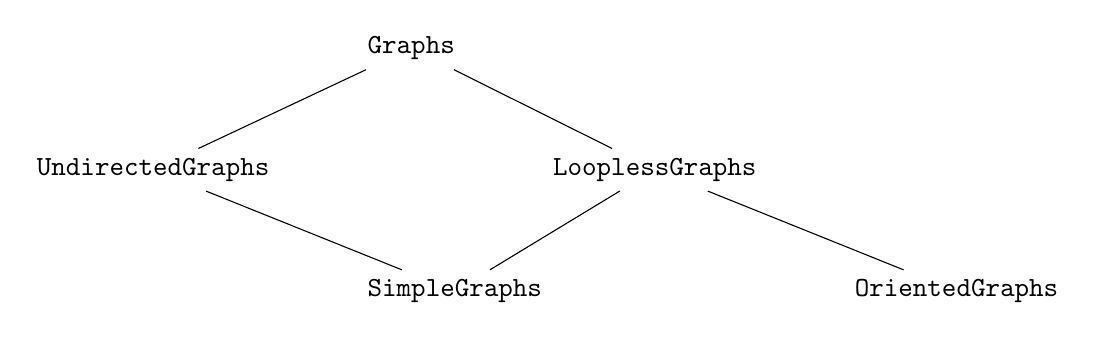
\begin{tikzpicture}[category/.style={font=\ttfamily}] \node (UG) [category]
{UndirectedGraphs}; \node (G) [category, above right=of UG] {Graphs}; \node
(SG) [category, below right=of UG] {SimpleGraphs}; \node (LG) [category, below
right=of G] {LooplessGraphs}; \node (OG) [category, below right=of LG]
{OrientedGraphs}; \draw (UG) -- (G) -- (LG) -- (OG); \draw (UG) -- (SG) --
(LG); \end{tikzpicture}  
\begin{Verbatim}[commandchars=!@|,fontsize=\small,frame=single,label=Example]
  !gapprompt@gap>| !gapinput@g1:=CompleteGraph(2:GraphCategory:=SimpleGraphs);  |
  Graph( Category := SimpleGraphs, Order := 2, Size := 
  1, Adjacencies := [ [ 2 ], [ 1 ] ] )
  !gapprompt@gap>| !gapinput@g2:=CompleteGraph(2:GraphCategory:=OrientedGraphs);|
  Graph( Category := OrientedGraphs, Order := 2, Size := 
  1, Adjacencies := [ [ 2 ], [  ] ] )
  !gapprompt@gap>| !gapinput@g3:=CompleteGraph(2:GraphCategory:=UndirectedGraphs);|
  Graph( Category := UndirectedGraphs, Order := 2, Size := 
  3, Adjacencies := [ [ 1, 2 ], [ 1, 2 ] ] )
  !gapprompt@gap>| !gapinput@GraphCategory([g1,g2,g3]);|
  <Category "Graphs">
  !gapprompt@gap>| !gapinput@GraphCategory([g1,g2]);   |
  <Category "LooplessGraphs">
  !gapprompt@gap>| !gapinput@GraphCategory([g1,g3]);|
  <Category "UndirectedGraphs">
\end{Verbatim}
 }

 

\subsection{\textcolor{Chapter }{Graphs}}
\logpage{[ "B", 1, 75 ]}\nobreak
\hyperdef{L}{X815691877F8C800C}{}
{\noindent\textcolor{FuncColor}{$\triangleright$\ \ \texttt{Graphs({\mdseries\slshape G})\index{Graphs@\texttt{Graphs}}
\label{Graphs}
}\hfill{\scriptsize (function)}}\\


 \texttt{Graphs} is the most general graph category in \textsf{YAGS}. This category contains all graphs that can be represented in \textsf{YAGS}. A graph in this category may contain loops, arrows and edges (which in \textsf{YAGS} are exactly the same as two opposite arrows between some pair of vertices).
This graph category has no parent category. 
\begin{Verbatim}[commandchars=!@|,fontsize=\small,frame=single,label=Example]
  !gapprompt@gap>| !gapinput@GraphByWalks([1,1],[1,2],[2,1],[3,2]:GraphCategory:=Graphs);|
  Graph( Category := Graphs, Order := 3, Size := 4, Adjacencies := 
  [ [ 1, 2 ], [ 1 ], [ 2 ] ] )
  !gapprompt@gap>| !gapinput@GraphByWalks([1,1],[1,2],[2,1],[3,2]:GraphCategory:=SimpleGraphs);  |
  Graph( Category := SimpleGraphs, Order := 3, Size := 
  2, Adjacencies := [ [ 2 ], [ 1, 3 ], [ 2 ] ] )
\end{Verbatim}
 }

 

\subsection{\textcolor{Chapter }{GraphsOfGivenOrder}}
\logpage{[ "B", 1, 76 ]}\nobreak
\hyperdef{L}{X7F66DFB17CC3B2D9}{}
{\noindent\textcolor{FuncColor}{$\triangleright$\ \ \texttt{GraphsOfGivenOrder({\mdseries\slshape n})\index{GraphsOfGivenOrder@\texttt{GraphsOfGivenOrder}}
\label{GraphsOfGivenOrder}
}\hfill{\scriptsize (operation)}}\\


 

Returns the list of all graphs of order \mbox{\texttt{\mdseries\slshape n}} (upto isomorphism). This operation uses Brendan McKay's data published here: \href{https://cs.anu.edu.au/people/Brendan.McKay/data/graphs.html} {\texttt{https://cs.anu.edu.au/people/Brendan.McKay/data/graphs.html}}. 

These data are included with the \textsf{YAGS} distribution in its \texttt{data} directory. Hence this operation simply reads the corresponding file in that
directory using \texttt{ImportGraph6( \mbox{\texttt{\mdseries\slshape Filename}} )}. Therefore, the integer \mbox{\texttt{\mdseries\slshape n}} must be in the range from 1 upto 9. Data for graphs on 10 vertices is also
available, but not included with \textsf{YAGS}, it may not be practical to use that data, but if you would like to try, all
you have to do is to copy (and to uncompress) the corresponding file into the
directory \texttt{\mbox{\texttt{\mdseries\slshape YAGS-DIR}}/data}. 
\begin{Verbatim}[commandchars=!@|,fontsize=\small,frame=single,label=Example]
  !gapprompt@gap>| !gapinput@GraphsOfGivenOrder(2);          |
  [ Graph( Category := SimpleGraphs, Order := 2, Size := 
      0, Adjacencies := [ [  ], [  ] ] ), 
    Graph( Category := SimpleGraphs, Order := 2, Size := 
      1, Adjacencies := [ [ 2 ], [ 1 ] ] ) ]
  !gapprompt@gap>| !gapinput@GraphsOfGivenOrder(3);|
  [ Graph( Category := SimpleGraphs, Order := 3, Size := 
      0, Adjacencies := [ [  ], [  ], [  ] ] ), 
    Graph( Category := SimpleGraphs, Order := 3, Size := 
      1, Adjacencies := [ [ 3 ], [  ], [ 1 ] ] ), 
    Graph( Category := SimpleGraphs, Order := 3, Size := 
      2, Adjacencies := [ [ 3 ], [ 3 ], [ 1, 2 ] ] ), 
    Graph( Category := SimpleGraphs, Order := 3, Size := 
      3, Adjacencies := [ [ 2, 3 ], [ 1, 3 ], [ 1, 2 ] ] ) ]
  !gapprompt@gap>| !gapinput@Length(GraphsOfGivenOrder(9));|
  274668
  !gapprompt@gap>| !gapinput@GraphsOfGivenOrder(10);       |
  #W Unreadable File: /opt/gap4r7/pkg/yags/data/graph10.g6
  fail
\end{Verbatim}
 }

 

\subsection{\textcolor{Chapter }{GraphSum}}
\logpage{[ "B", 1, 77 ]}\nobreak
\hyperdef{L}{X7E8B61AD787C430F}{}
{\noindent\textcolor{FuncColor}{$\triangleright$\ \ \texttt{GraphSum({\mdseries\slshape G, L})\index{GraphSum@\texttt{GraphSum}}
\label{GraphSum}
}\hfill{\scriptsize (operation)}}\\


 

Returns the lexicographic sum of a list of graphs \mbox{\texttt{\mdseries\slshape L}} over a graph \mbox{\texttt{\mdseries\slshape G}}. 

The lexicographic sum is computed as follows: 

Given \mbox{\texttt{\mdseries\slshape G}}, with $Order(G)=n$ and a list of \mbox{\texttt{\mdseries\slshape n}} graphs $L = [G_1, \ldots, G_n]$, We take the disjoint union of $G_1,G_2, \ldots,G_n$ and then we add all the edges between $G_i$ and $G_j$ whenever $[i,j]$ is and edge of $G$. 

If \mbox{\texttt{\mdseries\slshape L}} contains holes, the trivial graph is used in place. 
\begin{Verbatim}[commandchars=!@|,fontsize=\small,frame=single,label=Example]
  !gapprompt@gap>| !gapinput@t:=TrivialGraph;; g:=CycleGraph(4);;|
  !gapprompt@gap>| !gapinput@GraphSum(PathGraph(3),[t,g,t]);|
  Graph( Category := SimpleGraphs, Order := 6, Size := 
  12, Adjacencies := [ [ 2, 3, 4, 5 ], [ 1, 3, 5, 6 ], [ 1, 2, 4, 6 ], 
    [ 1, 3, 5, 6 ], [ 1, 2, 4, 6 ], [ 2, 3, 4, 5 ] ] )
  !gapprompt@gap>| !gapinput@GraphSum(PathGraph(3),[,g,]);  |
  Graph( Category := SimpleGraphs, Order := 6, Size := 
  12, Adjacencies := [ [ 2, 3, 4, 5 ], [ 1, 3, 5, 6 ], [ 1, 2, 4, 6 ], 
    [ 1, 3, 5, 6 ], [ 1, 2, 4, 6 ], [ 2, 3, 4, 5 ] ] )
\end{Verbatim}
 }

 

\subsection{\textcolor{Chapter }{GraphToRaw}}
\logpage{[ "B", 1, 78 ]}\nobreak
\hyperdef{L}{X8661587880C12114}{}
{\noindent\textcolor{FuncColor}{$\triangleright$\ \ \texttt{GraphToRaw({\mdseries\slshape FileName, G})\index{GraphToRaw@\texttt{GraphToRaw}}
\label{GraphToRaw}
}\hfill{\scriptsize (operation)}}\\


 

Converts a \textsf{YAGS} graph \mbox{\texttt{\mdseries\slshape G}} into a raw format (number of vertices, coordinates and adjacency matrix) and
writes the converted data to the file \mbox{\texttt{\mdseries\slshape FileName}}. For use by the external program \texttt{draw} (see \texttt{Draw(\mbox{\texttt{\mdseries\slshape G}})} ). 
\begin{Verbatim}[commandchars=!@|,fontsize=\small,frame=single,label=Example]
  !gapprompt@gap>| !gapinput@g:=CycleGraph(4);;|
  !gapprompt@gap>| !gapinput@GraphToRaw("mygraph.raw",g);|
\end{Verbatim}
 }

 

\subsection{\textcolor{Chapter }{GraphUpdateFromRaw}}
\logpage{[ "B", 1, 79 ]}\nobreak
\hyperdef{L}{X793E67DD83402749}{}
{\noindent\textcolor{FuncColor}{$\triangleright$\ \ \texttt{GraphUpdateFromRaw({\mdseries\slshape FileName, G})\index{GraphUpdateFromRaw@\texttt{GraphUpdateFromRaw}}
\label{GraphUpdateFromRaw}
}\hfill{\scriptsize (operation)}}\\


 

Updates the coordinates of \mbox{\texttt{\mdseries\slshape G}} from a file \mbox{\texttt{\mdseries\slshape FileName}} in raw format. Intended for internal use only. }

 

\subsection{\textcolor{Chapter }{GroupGraph}}
\logpage{[ "B", 1, 80 ]}\nobreak
\hyperdef{L}{X78BA06B387DA3279}{}
{\noindent\textcolor{FuncColor}{$\triangleright$\ \ \texttt{GroupGraph({\mdseries\slshape G, Grp, Act})\index{GroupGraph@\texttt{GroupGraph}}
\label{GroupGraph}
}\hfill{\scriptsize (operation)}}\\
\noindent\textcolor{FuncColor}{$\triangleright$\ \ \texttt{GroupGraph({\mdseries\slshape G, Grp})\index{GroupGraph@\texttt{GroupGraph}}
\label{GroupGraph}
}\hfill{\scriptsize (operation)}}\\


 

Given a graph \mbox{\texttt{\mdseries\slshape G}}, a group \mbox{\texttt{\mdseries\slshape Grp}} and an action \mbox{\texttt{\mdseries\slshape Act}} of \mbox{\texttt{\mdseries\slshape Grp}} on some set S which contains $Vertices( \mbox{\texttt{\mdseries\slshape G}} )$, \texttt{GroupGraph} returns a new graph with vertex set $\{\mbox{\texttt{\mdseries\slshape Act}}(v,g) : g \in \mbox{\texttt{\mdseries\slshape Grp}}, v \in Vertices( \mbox{\texttt{\mdseries\slshape G}} )\}$ and edge set $\{\{\mbox{\texttt{\mdseries\slshape Act}}(v,g),\mbox{\texttt{\mdseries\slshape Act}}(u,g)\}: g\in \mbox{\texttt{\mdseries\slshape Grp}}, \{u,v\}\in Edges( \mbox{\texttt{\mdseries\slshape G}} )\}$. 

If \mbox{\texttt{\mdseries\slshape Act}} is omited, the standard \textsf{GAP} action \texttt{OnPoints} is used. 
\begin{Verbatim}[commandchars=!@|,fontsize=\small,frame=single,label=Example]
  !gapprompt@gap>| !gapinput@GroupGraph(GraphByWalks([1,2]),Group([(1,2,3,4,5),(2,5)(3,4)]));|
  Graph( Category := SimpleGraphs, Order := 5, Size := 
  5, Adjacencies := [ [ 2, 5 ], [ 1, 3 ], [ 2, 4 ], [ 3, 5 ], [ 1, 4 ] 
   ] )
\end{Verbatim}
 }

 

\subsection{\textcolor{Chapter }{HararyToMcKay}}
\logpage{[ "B", 1, 81 ]}\nobreak
\hyperdef{L}{X82276E097B77591E}{}
{\noindent\textcolor{FuncColor}{$\triangleright$\ \ \texttt{HararyToMcKay({\mdseries\slshape Spec})\index{HararyToMcKay@\texttt{HararyToMcKay}}
\label{HararyToMcKay}
}\hfill{\scriptsize (operation)}}\\
\noindent\textcolor{FuncColor}{$\triangleright$\ \ \texttt{McKayToHarary({\mdseries\slshape index})\index{McKayToHarary@\texttt{McKayToHarary}}
\label{McKayToHarary}
}\hfill{\scriptsize (operation)}}\\


 

Returns the McKay's \mbox{\texttt{\mdseries\slshape index}} of a Harary's graph specification \mbox{\texttt{\mdseries\slshape Spec}} and viceversa. Frank Harary published in his book \cite{Har69}, a list af all 208 simple graphs of order upto 6 (upto isomorphism). Each of
them had a label (which we call \mbox{\texttt{\mdseries\slshape Harary's graph specification}}) of the form \texttt{[ \mbox{\texttt{\mdseries\slshape n}}, \mbox{\texttt{\mdseries\slshape m}}, \mbox{\texttt{\mdseries\slshape s}} ]} where \mbox{\texttt{\mdseries\slshape n}} is the number of vertices, \mbox{\texttt{\mdseries\slshape m}} is the number of edges, and \mbox{\texttt{\mdseries\slshape s}} is a consecutive integer which uniquely identifies the graph from the others
with the same \mbox{\texttt{\mdseries\slshape n}} and \mbox{\texttt{\mdseries\slshape m}}. On the other hand, Brendan McKay published data sets containing a list of
all graphs of order upto 10 (also upto isomorphism), here: 

\href{https://cs.anu.edu.au/people/Brendan.McKay/data/graphs.html} {\texttt{https://cs.anu.edu.au/people/Brendan.McKay/data/graphs.html}} 

Each graph in these data sets appears in some specific position (which we call \emph{McKay's index}). We found it convenient to have an automated way to convert from Harary's
graph specifications to McKay's indexes and viceversa. 
\begin{Verbatim}[commandchars=!@|,fontsize=\small,frame=single,label=Example]
  !gapprompt@gap>| !gapinput@HararyToMcKay([1,0,1]); |
  1
  !gapprompt@gap>| !gapinput@HararyToMcKay([1,0,2]);|
  fail
  !gapprompt@gap>| !gapinput@HararyToMcKay([5,5,2]);|
  31
  !gapprompt@gap>| !gapinput@HararyToMcKay([5,5,3]);|
  34
  !gapprompt@gap>| !gapinput@HararyToMcKay([5,5,5]);|
  30
  !gapprompt@gap>| !gapinput@HararyToMcKay([5,5,6]);|
  45
  !gapprompt@gap>| !gapinput@HararyToMcKay([5,5,7]); |
  fail
  !gapprompt@gap>| !gapinput@HararyToMcKay([6,15,1]);|
  208
  !gapprompt@gap>| !gapinput@HararyToMcKay([6,15,2]);|
  fail
\end{Verbatim}
 
\begin{Verbatim}[commandchars=!@|,fontsize=\small,frame=single,label=Example]
  !gapprompt@gap>| !gapinput@List([1..208],McKayToHarary);|
  [ [ 1, 0, 1 ], [ 2, 0, 1 ], [ 2, 1, 1 ], [ 3, 0, 1 ], [ 3, 1, 1 ], 
    [ 3, 2, 1 ], [ 3, 3, 1 ], [ 4, 0, 1 ], [ 4, 1, 1 ], [ 4, 2, 1 ], 
    [ 4, 3, 3 ], [ 4, 2, 2 ], [ 4, 3, 1 ], [ 4, 3, 2 ], [ 4, 4, 1 ], 
  
                 --- many more lines here ---   
  
    [ 6, 10, 10 ], [ 6, 10, 7 ], [ 6, 11, 3 ], [ 6, 12, 1 ], [ 6, 13, 1 ], 
    [ 6, 11, 7 ], [ 6, 11, 9 ], [ 6, 11, 8 ], [ 6, 12, 4 ], [ 6, 12, 5 ], 
    [ 6, 13, 2 ], [ 6, 14, 1 ], [ 6, 15, 1 ] ]
\end{Verbatim}
 }

 

\subsection{\textcolor{Chapter }{HouseGraph}}
\logpage{[ "B", 1, 82 ]}\nobreak
\hyperdef{L}{X7FA941E678EAA379}{}
{\noindent\textcolor{FuncColor}{$\triangleright$\ \ \texttt{HouseGraph\index{HouseGraph@\texttt{HouseGraph}}
\label{HouseGraph}
}\hfill{\scriptsize (global variable)}}\\


 

A 4-Cycle and a triangle glued by an edge. 
\begin{Verbatim}[commandchars=!@|,fontsize=\small,frame=single,label=Example]
  !gapprompt@gap>| !gapinput@HouseGraph;|
  Graph( Category := SimpleGraphs, Order := 5, Size := 
  6, Adjacencies := [ [ 2, 4, 5 ], [ 1, 3 ], [ 2, 4 ], [ 1, 3, 5 ], 
    [ 1, 4 ] ] )
\end{Verbatim}
 }

 

\subsection{\textcolor{Chapter }{Icosahedron}}
\logpage{[ "B", 1, 83 ]}\nobreak
\hyperdef{L}{X83E0EF8F7CCD6979}{}
{\noindent\textcolor{FuncColor}{$\triangleright$\ \ \texttt{Icosahedron\index{Icosahedron@\texttt{Icosahedron}}
\label{Icosahedron}
}\hfill{\scriptsize (global variable)}}\\


 

The 1-skeleton of Plato's icosahedron. 
\begin{Verbatim}[commandchars=!@|,fontsize=\small,frame=single,label=Example]
  !gapprompt@gap>| !gapinput@Icosahedron;|
  Graph( Category := SimpleGraphs, Order := 12, Size := 
  30, Adjacencies := [ [ 2, 3, 4, 5, 6 ], [ 1, 3, 6, 9, 10 ], 
    [ 1, 2, 4, 10, 11 ], [ 1, 3, 5, 7, 11 ], [ 1, 4, 6, 7, 8 ], 
    [ 1, 2, 5, 8, 9 ], [ 4, 5, 8, 11, 12 ], [ 5, 6, 7, 9, 12 ], 
    [ 2, 6, 8, 10, 12 ], [ 2, 3, 9, 11, 12 ], [ 3, 4, 7, 10, 12 ], 
    [ 7, 8, 9, 10, 11 ] ] )
\end{Verbatim}
 }

 

\subsection{\textcolor{Chapter }{ImportGraph6}}
\logpage{[ "B", 1, 84 ]}\nobreak
\hyperdef{L}{X7DF0F8C079D7D07D}{}
{\noindent\textcolor{FuncColor}{$\triangleright$\ \ \texttt{ImportGraph6({\mdseries\slshape Filename})\index{ImportGraph6@\texttt{ImportGraph6}}
\label{ImportGraph6}
}\hfill{\scriptsize (operation)}}\\


 

Returns the list of graphs represented in \mbox{\texttt{\mdseries\slshape Filename}} which are encoded using Brendan McKay's graph6 format. This operation allows
us to read data in databases which use this format. Several such databases can
be found here: \href{https://cs.anu.edu.au/people/Brendan.McKay/data/graphs.html} {\texttt{https://cs.anu.edu.au/people/Brendan.McKay/data/graphs.html}}. 

The graph6 format is described here: 

\href{https://cs.anu.edu.au/people/Brendan.McKay/data/formats.txt} {\texttt{https://cs.anu.edu.au/people/Brendan.McKay/data/formats.txt}}. 

The following example assumes that you have a file named \texttt{graph3.g6} in your working directory which encodes graphs in graph6 format; the contents
of this file is assumed to be as indicated after the first command in the
example. It is also assumed that your Operative System is a Unix-like system. 
\begin{Verbatim}[commandchars=!@|,fontsize=\small,frame=single,label=Example]
  !gapprompt@gap>| !gapinput@Exec("cat graph3.g6");|
  B?
  BO
  BW
  Bw
  !gapprompt@gap>| !gapinput@ImportGraph6("graph3.g6");|
  [ Graph( Category := SimpleGraphs, Order := 3, Size := 0, Adjacencies := 
      [ [  ], [  ], [  ] ] ), Graph( Category := SimpleGraphs, Order := 
      3, Size := 1, Adjacencies := [ [ 3 ], [  ], [ 1 ] ] ), 
    Graph( Category := SimpleGraphs, Order := 3, Size := 2, Adjacencies := 
      [ [ 3 ], [ 3 ], [ 1, 2 ] ] ), Graph( Category := SimpleGraphs, Order :=
     3, Size := 3, Adjacencies := [ [ 2, 3 ], [ 1, 3 ], [ 1, 2 ] ] ) ]
\end{Verbatim}
 }

 

\subsection{\textcolor{Chapter }{in}}
\logpage{[ "B", 1, 85 ]}\nobreak
\hyperdef{L}{X87BDB89B7AAFE8AD}{}
{\noindent\textcolor{FuncColor}{$\triangleright$\ \ \texttt{in({\mdseries\slshape G, Catgy})\index{in@\texttt{in}}
\label{in}
}\hfill{\scriptsize (operation)}}\\


 

Returns \texttt{true} if graph \mbox{\texttt{\mdseries\slshape G}} belongs to category \mbox{\texttt{\mdseries\slshape Catgy}} and \texttt{false} otherwise. 
\begin{Verbatim}[commandchars=!@|,fontsize=\small,frame=single,label=Example]
  !gapprompt@gap>| !gapinput@g:=WheelGraph(4);|
  Graph( Category := SimpleGraphs, Order := 5, Size := 
  8, Adjacencies := [ [ 2, 3, 4, 5 ], [ 1, 3, 5 ], [ 1, 2, 4 ], 
    [ 1, 3, 5 ], [ 1, 2, 4 ] ] )
  !gapprompt@gap>| !gapinput@g in SimpleGraphs;|
  true
  !gapprompt@gap>| !gapinput@g in Graphs;|
  true
  !gapprompt@gap>| !gapinput@g in OrientedGraphs;|
  false
\end{Verbatim}
 }

 

\subsection{\textcolor{Chapter }{InducedSubgraph}}
\logpage{[ "B", 1, 86 ]}\nobreak
\hyperdef{L}{X7D9F576185C58545}{}
{\noindent\textcolor{FuncColor}{$\triangleright$\ \ \texttt{InducedSubgraph({\mdseries\slshape G, V})\index{InducedSubgraph@\texttt{InducedSubgraph}}
\label{InducedSubgraph}
}\hfill{\scriptsize (operation)}}\\


 

Returns the subgraph of graph \mbox{\texttt{\mdseries\slshape G}} induced by the vertex set \mbox{\texttt{\mdseries\slshape V}}. 
\begin{Verbatim}[commandchars=!@|,fontsize=\small,frame=single,label=Example]
  !gapprompt@gap>| !gapinput@g:=CycleGraph(6);          |
  Graph( Category := SimpleGraphs, Order := 6, Size := 
  6, Adjacencies := [ [ 2, 6 ], [ 1, 3 ], [ 2, 4 ], [ 3, 5 ], [ 4, 6 ], 
    [ 1, 5 ] ] )
  !gapprompt@gap>| !gapinput@InducedSubgraph(g,[3,4,6]);  |
  Graph( Category := SimpleGraphs, Order := 3, Size := 
  1, Adjacencies := [ [ 2 ], [ 1 ], [  ] ] )
\end{Verbatim}
 

The order of the elements in \mbox{\texttt{\mdseries\slshape V}} does matter. 
\begin{Verbatim}[commandchars=!@|,fontsize=\small,frame=single,label=Example]
  !gapprompt@gap>| !gapinput@InducedSubgraph(g,[6,3,4]);  |
  Graph( Category := SimpleGraphs, Order := 3, Size := 
  1, Adjacencies := [ [  ], [ 3 ], [ 2 ] ] )
\end{Verbatim}
 }

 

\subsection{\textcolor{Chapter }{InNeigh}}
\logpage{[ "B", 1, 87 ]}\nobreak
\hyperdef{L}{X78318B95813CAA26}{}
{\noindent\textcolor{FuncColor}{$\triangleright$\ \ \texttt{InNeigh({\mdseries\slshape G, x})\index{InNeigh@\texttt{InNeigh}}
\label{InNeigh}
}\hfill{\scriptsize (operation)}}\\


 

Returns the list of in-neighbors of \mbox{\texttt{\mdseries\slshape x}} in \mbox{\texttt{\mdseries\slshape G}}. 
\begin{Verbatim}[commandchars=!@|,fontsize=\small,frame=single,label=Example]
  !gapprompt@gap>| !gapinput@tt:=CompleteGraph(5:GraphCategory:=OrientedGraphs);|
  Graph( Category := OrientedGraphs, Order := 5, Size := 
  10, Adjacencies := [ [ 2, 3, 4, 5 ], [ 3, 4, 5 ], [ 4, 5 ], [ 5 ], 
    [  ] ] )
  !gapprompt@gap>| !gapinput@InNeigh(tt,3);                                     |
  [ 1, 2 ]
  !gapprompt@gap>| !gapinput@OutNeigh(tt,3);                                    |
  [ 4, 5 ]
\end{Verbatim}
 }

 

\subsection{\textcolor{Chapter }{InteriorVertices}}
\logpage{[ "B", 1, 88 ]}\nobreak
\hyperdef{L}{X7F43E2F0802FD790}{}
{\noindent\textcolor{FuncColor}{$\triangleright$\ \ \texttt{InteriorVertices({\mdseries\slshape G})\index{InteriorVertices@\texttt{InteriorVertices}}
\label{InteriorVertices}
}\hfill{\scriptsize (attribute)}}\\


 

When \mbox{\texttt{\mdseries\slshape G}} is a compact surface, it returns the list of vertices in the interior (of the
triangulation) of the surface. That is, the list of vertices of \mbox{\texttt{\mdseries\slshape G}} that have links isomorphic to a cycle. It returns \texttt{fail} if \mbox{\texttt{\mdseries\slshape G}} is not a compact surface. 
\begin{Verbatim}[commandchars=!@|,fontsize=\small,frame=single,label=Example]
  !gapprompt@gap>| !gapinput@InteriorVertices(WheelGraph(4,2));|
  [ 1, 2, 3, 4, 5 ]
  !gapprompt@gap>| !gapinput@InteriorVertices(Octahedron);     |
  [ 1, 2, 3, 4, 5, 6 ]
\end{Verbatim}
 }

 

\subsection{\textcolor{Chapter }{IntersectionGraph}}
\logpage{[ "B", 1, 89 ]}\nobreak
\hyperdef{L}{X827067C078A10B24}{}
{\noindent\textcolor{FuncColor}{$\triangleright$\ \ \texttt{IntersectionGraph({\mdseries\slshape L})\index{IntersectionGraph@\texttt{IntersectionGraph}}
\label{IntersectionGraph}
}\hfill{\scriptsize (function)}}\\


 

Returns the intersection graph of the family of sets \mbox{\texttt{\mdseries\slshape L}}. This graph has a vertex for every set in \mbox{\texttt{\mdseries\slshape L}}, and two such vertices are adjacent iff the corresponding sets have non-empty
intersection. 
\begin{Verbatim}[commandchars=!@|,fontsize=\small,frame=single,label=Example]
  !gapprompt@gap>| !gapinput@IntersectionGraph([[1,2,3],[3,4,5],[5,6,7]]);|
  Graph( Category := SimpleGraphs, Order := 3, Size := 
  2, Adjacencies := [ [ 2 ], [ 1, 3 ], [ 2 ] ] )
\end{Verbatim}
 }

 

\subsection{\textcolor{Chapter }{IsBoolean}}
\logpage{[ "B", 1, 90 ]}\nobreak
\hyperdef{L}{X80FF64FC7E750046}{}
{\noindent\textcolor{FuncColor}{$\triangleright$\ \ \texttt{IsBoolean({\mdseries\slshape Obj})\index{IsBoolean@\texttt{IsBoolean}}
\label{IsBoolean}
}\hfill{\scriptsize (function)}}\\


 

Returns \texttt{true} if object \mbox{\texttt{\mdseries\slshape Obj}} is \texttt{true} or \texttt{false} and \texttt{false} otherwise. 
\begin{Verbatim}[commandchars=!@|,fontsize=\small,frame=single,label=Example]
  !gapprompt@gap>| !gapinput@IsBoolean( true ); IsBoolean( fail ); IsBoolean ( false );|
  true
  false
  true
\end{Verbatim}
 }

 

\subsection{\textcolor{Chapter }{IsCliqueGated}}
\logpage{[ "B", 1, 91 ]}\nobreak
\hyperdef{L}{X78F70A8B7C72464C}{}
{\noindent\textcolor{FuncColor}{$\triangleright$\ \ \texttt{IsCliqueGated({\mdseries\slshape G})\index{IsCliqueGated@\texttt{IsCliqueGated}}
\label{IsCliqueGated}
}\hfill{\scriptsize (property)}}\\


 

Returns \texttt{true} if \mbox{\texttt{\mdseries\slshape G}} is a clique gated graph \cite{HK96}. }

 

\subsection{\textcolor{Chapter }{IsCliqueHelly}}
\logpage{[ "B", 1, 92 ]}\nobreak
\hyperdef{L}{X822B38D686BC1D2D}{}
{\noindent\textcolor{FuncColor}{$\triangleright$\ \ \texttt{IsCliqueHelly({\mdseries\slshape G})\index{IsCliqueHelly@\texttt{IsCliqueHelly}}
\label{IsCliqueHelly}
}\hfill{\scriptsize (property)}}\\


 

Returns \texttt{true} if the set of (maximal) cliques \mbox{\texttt{\mdseries\slshape G}} satisfy the \emph{Helly} property. 

The Helly property is defined as follows: 

A non-empty family $F$ of non-empty sets satisfies the Helly property if every pairwise intersecting
subfamily of $F$ has a non-empty total intersection. 

Here we use the Dragan-Szwarcfiter characterization \cite{Dra89}\cite{Szw97} to compute the Helly property. 
\begin{Verbatim}[commandchars=!@|,fontsize=\small,frame=single,label=Example]
  !gapprompt@gap>| !gapinput@g:=SunGraph(3);|
  Graph( Category := SimpleGraphs, Order := 6, Size := 
  9, Adjacencies := [ [ 2, 6 ], [ 1, 3, 4, 6 ], [ 2, 4 ], 
    [ 2, 3, 5, 6 ], [ 4, 6 ], [ 1, 2, 4, 5 ] ] )
  !gapprompt@gap>| !gapinput@IsCliqueHelly(g);|
  false
\end{Verbatim}
 }

 

\subsection{\textcolor{Chapter }{IsCompactSurface}}
\logpage{[ "B", 1, 93 ]}\nobreak
\hyperdef{L}{X8563061F83E10A23}{}
{\noindent\textcolor{FuncColor}{$\triangleright$\ \ \texttt{IsCompactSurface({\mdseries\slshape G})\index{IsCompactSurface@\texttt{IsCompactSurface}}
\label{IsCompactSurface}
}\hfill{\scriptsize (property)}}\\


 

Returns \texttt{true} if every link of \mbox{\texttt{\mdseries\slshape G}} is either an \mbox{\texttt{\mdseries\slshape n}}-cycle, for $n\geq 4$ or an \mbox{\texttt{\mdseries\slshape m}}-path, for $m\geq 2$. (not necessarily the same \mbox{\texttt{\mdseries\slshape n}}/\mbox{\texttt{\mdseries\slshape m}} for all vertices); it returns \texttt{false} otherwise. 

This notion correspond to Whitney triangulations of compact surfaces \cite{LNP02} in which the (maximal) cliques of the graph are exactly the triangles of the
triangulation. 
\begin{Verbatim}[commandchars=!@|,fontsize=\small,frame=single,label=Example]
  !gapprompt@gap>| !gapinput@IsCompactSurface(Icosahedron);                             |
  true
  !gapprompt@gap>| !gapinput@IsCompactSurface(RemoveVertices(Icosahedron,[1]));|
  true
  !gapprompt@gap>| !gapinput@IsCompactSurface(WheelGraph(4,2));|
  true
  !gapprompt@gap>| !gapinput@IsCompactSurface(Tetrahedron);    |
  false
  !gapprompt@gap>| !gapinput@IsCompactSurface(CompleteGraph(2));|
  false
  !gapprompt@gap>| !gapinput@IsCompactSurface(CompleteGraph(3));|
  true
  !gapprompt@gap>| !gapinput@IsCompactSurface(CompleteGraph(4));|
  false
\end{Verbatim}
 

Topologically, the difference between a surface and a compact surface is that
the points of a surface always have a open neighborhood homeomorphic to an
open disk, whereas a compact surface may also contain points with open
neighborhoods homeomorphic to a closed half-plane. }

 

\subsection{\textcolor{Chapter }{IsComplete}}
\logpage{[ "B", 1, 94 ]}\nobreak
\hyperdef{L}{X7D689F21828A4278}{}
{\noindent\textcolor{FuncColor}{$\triangleright$\ \ \texttt{IsComplete({\mdseries\slshape G, L})\index{IsComplete@\texttt{IsComplete}}
\label{IsComplete}
}\hfill{\scriptsize (operation)}}\\


 

Returns \texttt{true} if \mbox{\texttt{\mdseries\slshape L}} induces a complete subgraph of \mbox{\texttt{\mdseries\slshape G}}. 
\begin{Verbatim}[commandchars=!@|,fontsize=\small,frame=single,label=Example]
  !gapprompt@gap>| !gapinput@IsComplete(DiamondGraph,[1,2,3]);|
  true
  !gapprompt@gap>| !gapinput@IsComplete(DiamondGraph,[1,2,4]);|
  false
\end{Verbatim}
 }

 

\subsection{\textcolor{Chapter }{IsCompleteGraph}}
\logpage{[ "B", 1, 95 ]}\nobreak
\hyperdef{L}{X7BA6EF9F80968CD8}{}
{\noindent\textcolor{FuncColor}{$\triangleright$\ \ \texttt{IsCompleteGraph({\mdseries\slshape G})\index{IsCompleteGraph@\texttt{IsCompleteGraph}}
\label{IsCompleteGraph}
}\hfill{\scriptsize (property)}}\\


 

Returns \texttt{true} if graph \mbox{\texttt{\mdseries\slshape G}} is a complete graph, \texttt{false} otherwise. In a complete graph every pair of vertices is an edge. }

 

\subsection{\textcolor{Chapter }{IsDiamondFree}}
\logpage{[ "B", 1, 96 ]}\nobreak
\hyperdef{L}{X7D03ACD07C167E0F}{}
{\noindent\textcolor{FuncColor}{$\triangleright$\ \ \texttt{IsDiamondFree({\mdseries\slshape G})\index{IsDiamondFree@\texttt{IsDiamondFree}}
\label{IsDiamondFree}
}\hfill{\scriptsize (property)}}\\


 

Returns \texttt{true} if \mbox{\texttt{\mdseries\slshape G}} is free from induced diamonds, \texttt{false} otherwise. 
\begin{Verbatim}[commandchars=!@|,fontsize=\small,frame=single,label=Example]
  !gapprompt@gap>| !gapinput@IsDiamondFree(Cube);|
  true
  !gapprompt@gap>| !gapinput@IsDiamondFree(Octahedron);|
  false
\end{Verbatim}
 }

 

\subsection{\textcolor{Chapter }{IsEdge}}
\logpage{[ "B", 1, 97 ]}\nobreak
\hyperdef{L}{X7F50265D789C602C}{}
{\noindent\textcolor{FuncColor}{$\triangleright$\ \ \texttt{IsEdge({\mdseries\slshape G, x, y})\index{IsEdge@\texttt{IsEdge}}
\label{IsEdge}
}\hfill{\scriptsize (operation)}}\\
\noindent\textcolor{FuncColor}{$\triangleright$\ \ \texttt{IsEdge({\mdseries\slshape G[, x, y{\textgreater}]})\index{IsEdge@\texttt{IsEdge}}
\label{IsEdge}
}\hfill{\scriptsize (operation)}}\\


 

Returns \texttt{true} if [\mbox{\texttt{\mdseries\slshape x}},\mbox{\texttt{\mdseries\slshape y}}] is an edge of \mbox{\texttt{\mdseries\slshape G}}. 
\begin{Verbatim}[commandchars=!@|,fontsize=\small,frame=single,label=Example]
  !gapprompt@gap>| !gapinput@IsEdge(PathGraph(3),1,2);|
  true
  !gapprompt@gap>| !gapinput@IsEdge(PathGraph(3),[1,2]);|
  true
  !gapprompt@gap>| !gapinput@IsEdge(PathGraph(3),1,3);|
  false
  !gapprompt@gap>| !gapinput@IsEdge(PathGraph(3),[1,3]);|
  false
\end{Verbatim}
 

The first form, IsEdge(\mbox{\texttt{\mdseries\slshape G}}, \mbox{\texttt{\mdseries\slshape x}}, \mbox{\texttt{\mdseries\slshape y}}), is a bit faster and hence more suitable for use in algoritms which make
extensive use of this operation. On the other hand, the first form does no
error checking at all, and hence, it may produce an error where the second
form returns false (for instance when \mbox{\texttt{\mdseries\slshape x}} is not a vertex of \mbox{\texttt{\mdseries\slshape G}}). The second form is therefore a bit slower, but more robust. 
\begin{Verbatim}[commandchars=!@|,fontsize=\small,frame=single,label=Example]
  !gapprompt@gap>| !gapinput@IsEdge(PathGraph(3),[7,3]);|
  false
  !gapprompt@gap>| !gapinput@IsEdge(PathGraph(3),7,3);  |
  Error, List Element: <list>[7] must have an assigned value
\end{Verbatim}
 }

 

\subsection{\textcolor{Chapter }{IsIsomorphicGraph}}
\logpage{[ "B", 1, 98 ]}\nobreak
\hyperdef{L}{X79CBEA7386509498}{}
{\noindent\textcolor{FuncColor}{$\triangleright$\ \ \texttt{IsIsomorphicGraph({\mdseries\slshape G, H})\index{IsIsomorphicGraph@\texttt{IsIsomorphicGraph}}
\label{IsIsomorphicGraph}
}\hfill{\scriptsize (operation)}}\\


 

Returns \texttt{true} when \mbox{\texttt{\mdseries\slshape G}} is isomorphic to \mbox{\texttt{\mdseries\slshape H}} and \texttt{false} otherwise. 
\begin{Verbatim}[commandchars=!@|,fontsize=\small,frame=single,label=Example]
  !gapprompt@gap>| !gapinput@g:=PowerGraph(CycleGraph(6),2);;h:=Octahedron;;|
  !gapprompt@gap>| !gapinput@IsIsomorphicGraph(g,h);|
  true
\end{Verbatim}
 }

 

\subsection{\textcolor{Chapter }{IsLocallyConstant}}
\logpage{[ "B", 1, 99 ]}\nobreak
\hyperdef{L}{X782871638792F4F5}{}
{\noindent\textcolor{FuncColor}{$\triangleright$\ \ \texttt{IsLocallyConstant({\mdseries\slshape G})\index{IsLocallyConstant@\texttt{IsLocallyConstant}}
\label{IsLocallyConstant}
}\hfill{\scriptsize (property)}}\\


 

Returns \texttt{true} if all the links of \mbox{\texttt{\mdseries\slshape G}} are isomorphic to each other; \texttt{false} otherwise. 
\begin{Verbatim}[commandchars=!@|,fontsize=\small,frame=single,label=Example]
  !gapprompt@gap>| !gapinput@IsLocallyConstant(PathGraph(2));|
  true
  !gapprompt@gap>| !gapinput@IsLocallyConstant(PathGraph(3));|
  false
  !gapprompt@gap>| !gapinput@IsLocallyConstant(CompleteGraph(3));|
  true
  !gapprompt@gap>| !gapinput@IsLocallyConstant(CycleGraph(4));   |
  true
  !gapprompt@gap>| !gapinput@IsLocallyConstant(Icosahedron);  |
  true
  !gapprompt@gap>| !gapinput@IsLocallyConstant(TorusGraph(5,4));|
  true
  !gapprompt@gap>| !gapinput@IsLocallyConstant(WheelGraph(4,2));|
  false
  !gapprompt@gap>| !gapinput@IsLocallyConstant(SnubDisphenoid); |
  false
\end{Verbatim}
 }

 

\subsection{\textcolor{Chapter }{IsLocallyH}}
\logpage{[ "B", 1, 100 ]}\nobreak
\hyperdef{L}{X7ACED06884FBC782}{}
{\noindent\textcolor{FuncColor}{$\triangleright$\ \ \texttt{IsLocallyH({\mdseries\slshape G, H})\index{IsLocallyH@\texttt{IsLocallyH}}
\label{IsLocallyH}
}\hfill{\scriptsize (operation)}}\\


 

Returns \texttt{true} if all the links of \mbox{\texttt{\mdseries\slshape G}} are isomorphic to \mbox{\texttt{\mdseries\slshape H}}; \texttt{false} otherwise. 
\begin{Verbatim}[commandchars=!@|,fontsize=\small,frame=single,label=Example]
  !gapprompt@gap>| !gapinput@IsLocallyH(Octahedron,CycleGraph(4));|
  true
  !gapprompt@gap>| !gapinput@IsLocallyH(Octahedron,CycleGraph(5));|
  false
  !gapprompt@gap>| !gapinput@IsLocallyH(Icosahedron,CycleGraph(5));|
  true
  !gapprompt@gap>| !gapinput@IsLocallyH(TorusGraph(4,4),CycleGraph(6));|
  true
\end{Verbatim}
 }

 

\subsection{\textcolor{Chapter }{IsLoopless}}
\logpage{[ "B", 1, 101 ]}\nobreak
\hyperdef{L}{X7F9F4622817E9AFB}{}
{\noindent\textcolor{FuncColor}{$\triangleright$\ \ \texttt{IsLoopless({\mdseries\slshape G})\index{IsLoopless@\texttt{IsLoopless}}
\label{IsLoopless}
}\hfill{\scriptsize (property)}}\\


 

Returns \texttt{true} if graph \mbox{\texttt{\mdseries\slshape G}} have no loops, \texttt{false} otherwise. Loops are edges from a vertex to itself. }

 

\subsection{\textcolor{Chapter }{IsoMorphism}}
\logpage{[ "B", 1, 102 ]}\nobreak
\hyperdef{L}{X80F38E797C303471}{}
{\noindent\textcolor{FuncColor}{$\triangleright$\ \ \texttt{IsoMorphism({\mdseries\slshape G, H})\index{IsoMorphism@\texttt{IsoMorphism}}
\label{IsoMorphism}
}\hfill{\scriptsize (operation)}}\\


 

Returns one isomorphism from \mbox{\texttt{\mdseries\slshape G}} to \mbox{\texttt{\mdseries\slshape H}} or \texttt{fail} if none exists. If \mbox{\texttt{\mdseries\slshape G}} has \mbox{\texttt{\mdseries\slshape n}} vertices, an isomorphisms $f : G\rightarrow H$ is represented as the list \texttt{\mbox{\texttt{\mdseries\slshape F}}=[f(1), f(2), ..., f(n)]}. 
\begin{Verbatim}[commandchars=!@|,fontsize=\small,frame=single,label=Example]
  !gapprompt@gap>| !gapinput@g:=CycleGraph(4);;h:=CompleteBipartiteGraph(2,2);;|
  !gapprompt@gap>| !gapinput@f:=IsoMorphism(g,h);|
  [ 1, 3, 2, 4 ]
\end{Verbatim}
 

See \texttt{NextIsoMorphism( \mbox{\texttt{\mdseries\slshape G}}, \mbox{\texttt{\mdseries\slshape H}}, \mbox{\texttt{\mdseries\slshape F}} )}. }

 

\subsection{\textcolor{Chapter }{IsoMorphisms}}
\logpage{[ "B", 1, 103 ]}\nobreak
\hyperdef{L}{X7D702EA087C1C5EF}{}
{\noindent\textcolor{FuncColor}{$\triangleright$\ \ \texttt{IsoMorphisms({\mdseries\slshape G, H})\index{IsoMorphisms@\texttt{IsoMorphisms}}
\label{IsoMorphisms}
}\hfill{\scriptsize (operation)}}\\


 

Returns the list of all isomorphism from \mbox{\texttt{\mdseries\slshape G}} to \mbox{\texttt{\mdseries\slshape H}}. If \mbox{\texttt{\mdseries\slshape G}} has \mbox{\texttt{\mdseries\slshape n}} vertices, an isomorphisms $f : G\rightarrow H$ is represented as the list \texttt{\mbox{\texttt{\mdseries\slshape F}}=[f(1), f(2), ..., f(n)]}. 
\begin{Verbatim}[commandchars=!@|,fontsize=\small,frame=single,label=Example]
  !gapprompt@gap>| !gapinput@g:=CycleGraph(4);;h:=CompleteBipartiteGraph(2,2);;|
  !gapprompt@gap>| !gapinput@IsoMorphisms(g,h);|
  [ [ 1, 3, 2, 4 ], [ 1, 4, 2, 3 ], [ 2, 3, 1, 4 ], [ 2, 4, 1, 3 ], 
    [ 3, 1, 4, 2 ], [ 3, 2, 4, 1 ], [ 4, 1, 3, 2 ], [ 4, 2, 3, 1 ] ]
\end{Verbatim}
 }

 

\subsection{\textcolor{Chapter }{IsOriented}}
\logpage{[ "B", 1, 104 ]}\nobreak
\hyperdef{L}{X8278D52F856A179D}{}
{\noindent\textcolor{FuncColor}{$\triangleright$\ \ \texttt{IsOriented({\mdseries\slshape G})\index{IsOriented@\texttt{IsOriented}}
\label{IsOriented}
}\hfill{\scriptsize (property)}}\\


 

Returns \texttt{true} if graph \mbox{\texttt{\mdseries\slshape G}} is an oriented graph, \texttt{false} otherwise. Regardless of the categories that \mbox{\texttt{\mdseries\slshape G}} belongs to, \mbox{\texttt{\mdseries\slshape G}} is oriented if whenever \texttt{[x,y]} is an edge of \mbox{\texttt{\mdseries\slshape G}}, \texttt{[y,x]} is not. }

 

\subsection{\textcolor{Chapter }{IsSimple}}
\logpage{[ "B", 1, 105 ]}\nobreak
\hyperdef{L}{X7D8E63A7824037CC}{}
{\noindent\textcolor{FuncColor}{$\triangleright$\ \ \texttt{IsSimple({\mdseries\slshape G})\index{IsSimple@\texttt{IsSimple}}
\label{IsSimple}
}\hfill{\scriptsize (property)}}\\


 

Returns \texttt{true} if graph \mbox{\texttt{\mdseries\slshape G}} is a simple graph, \texttt{false} otherwise. Regardless of the categories that \mbox{\texttt{\mdseries\slshape G}} belongs to, \mbox{\texttt{\mdseries\slshape G}} is simple if and only if \mbox{\texttt{\mdseries\slshape G}} is undirected and loopless. 

Returns \texttt{true} if the graph \mbox{\texttt{\mdseries\slshape G}} is simple regardless of its category. }

 

\subsection{\textcolor{Chapter }{IsSurface}}
\logpage{[ "B", 1, 106 ]}\nobreak
\hyperdef{L}{X8393259C7C8C4B73}{}
{\noindent\textcolor{FuncColor}{$\triangleright$\ \ \texttt{IsSurface({\mdseries\slshape G})\index{IsSurface@\texttt{IsSurface}}
\label{IsSurface}
}\hfill{\scriptsize (property)}}\\


 

Returns \texttt{true} if every link of \mbox{\texttt{\mdseries\slshape G}} is an \mbox{\texttt{\mdseries\slshape n}}-cycle, for $n\geq 4$ (not necessarily the same \mbox{\texttt{\mdseries\slshape n}} for all vertices); \texttt{false} otherwise. 

This notion correspond to Whitney triangulations of (closed) surfaces \cite{LNP02} in which the (maximal) cliques of the graph are exactly the triangles of the
triangulation. 
\begin{Verbatim}[commandchars=!@|,fontsize=\small,frame=single,label=Example]
  !gapprompt@gap>| !gapinput@IsSurface(SnubDisphenoid);|
  true
  !gapprompt@gap>| !gapinput@IsSurface(Icosahedron);   |
  true
  !gapprompt@gap>| !gapinput@IsSurface(RemoveVertices(Icosahedron,[1]));       |
  false
  !gapprompt@gap>| !gapinput@IsSurface(TorusGraph(4,5));|
  true
  !gapprompt@gap>| !gapinput@IsSurface(WheelGraph(4,2));|
  false
  !gapprompt@gap>| !gapinput@IsSurface(Tetrahedron);    |
  false
\end{Verbatim}
 

Topologically, the difference between a (closed) surface and a compact surface
is that the points of a surface always have a open neighborhood homeomorphic
to an open disk, whereas a compact surface may also contain points with open
neighborhoods homeomorphic to a closed half-plane. }

 

\subsection{\textcolor{Chapter }{IsTournament}}
\logpage{[ "B", 1, 107 ]}\nobreak
\hyperdef{L}{X7DD8D1A185EBE865}{}
{\noindent\textcolor{FuncColor}{$\triangleright$\ \ \texttt{IsTournament({\mdseries\slshape G})\index{IsTournament@\texttt{IsTournament}}
\label{IsTournament}
}\hfill{\scriptsize (property)}}\\


 

Returns \texttt{true} if \mbox{\texttt{\mdseries\slshape G}} is a tournament. 
\begin{Verbatim}[commandchars=!@|,fontsize=\small,frame=single,label=Example]
  !gapprompt@gap>| !gapinput@tt:=CompleteGraph(5:GraphCategory:=OrientedGraphs);|
  Graph( Category := OrientedGraphs, Order := 5, Size := 
  10, Adjacencies := [ [ 2, 3, 4, 5 ], [ 3, 4, 5 ], [ 4, 5 ], [ 5 ], 
    [  ] ] )
  !gapprompt@gap>| !gapinput@IsTournament(tt);                                  |
  true
\end{Verbatim}
 }

 

\subsection{\textcolor{Chapter }{IsTransitiveTournament}}
\logpage{[ "B", 1, 108 ]}\nobreak
\hyperdef{L}{X7CC7E10386094A61}{}
{\noindent\textcolor{FuncColor}{$\triangleright$\ \ \texttt{IsTransitiveTournament({\mdseries\slshape G})\index{IsTransitiveTournament@\texttt{IsTransitiveTournament}}
\label{IsTransitiveTournament}
}\hfill{\scriptsize (property)}}\\


 

Returns \texttt{true} if \mbox{\texttt{\mdseries\slshape G}} is a transitive tournament. 
\begin{Verbatim}[commandchars=!@|,fontsize=\small,frame=single,label=Example]
  !gapprompt@gap>| !gapinput@tt:=CompleteGraph(5:GraphCategory:=OrientedGraphs);|
  Graph( Category := OrientedGraphs, Order := 5, Size := 
  10, Adjacencies := [ [ 2, 3, 4, 5 ], [ 3, 4, 5 ], [ 4, 5 ], [ 5 ], 
    [  ] ] )
  !gapprompt@gap>| !gapinput@IsTransitiveTournament(tt);|
  true
\end{Verbatim}
 }

 

\subsection{\textcolor{Chapter }{IsUndirected}}
\logpage{[ "B", 1, 109 ]}\nobreak
\hyperdef{L}{X872108F17D8F264D}{}
{\noindent\textcolor{FuncColor}{$\triangleright$\ \ \texttt{IsUndirected({\mdseries\slshape G})\index{IsUndirected@\texttt{IsUndirected}}
\label{IsUndirected}
}\hfill{\scriptsize (property)}}\\


 

Returns \texttt{true} if graph \mbox{\texttt{\mdseries\slshape G}} is an undirected graph, \texttt{false} otherwise. Regardless of the categories that \mbox{\texttt{\mdseries\slshape G}} belongs to, \mbox{\texttt{\mdseries\slshape G}} is undirected if whenever \texttt{[x,y]} is an edge of \mbox{\texttt{\mdseries\slshape G}}, \texttt{[y,x]} is also an egde of \mbox{\texttt{\mdseries\slshape G}}. }

 

\subsection{\textcolor{Chapter }{JohnsonGraph}}
\logpage{[ "B", 1, 110 ]}\nobreak
\hyperdef{L}{X7A4036667F52738C}{}
{\noindent\textcolor{FuncColor}{$\triangleright$\ \ \texttt{JohnsonGraph({\mdseries\slshape n, r})\index{JohnsonGraph@\texttt{JohnsonGraph}}
\label{JohnsonGraph}
}\hfill{\scriptsize (function)}}\\


 

Returns the Johnson graph $J(n,r)$. The Johnson Graph is the graph whose vertices are \mbox{\texttt{\mdseries\slshape r}}-subset of the set $\{1, 2, \ldots, n\}$, two of them being adjacent iff they intersect in exactly \mbox{\texttt{\mdseries\slshape r}}-1 elements. 
\begin{Verbatim}[commandchars=!@|,fontsize=\small,frame=single,label=Example]
  !gapprompt@gap>| !gapinput@g:=JohnsonGraph(4,2);                                            |
  Graph( Category := SimpleGraphs, Order := 6, Size := 
  12, Adjacencies := [ [ 2, 3, 4, 5 ], [ 1, 3, 4, 6 ], [ 1, 2, 5, 6 ], 
    [ 1, 2, 5, 6 ], [ 1, 3, 4, 6 ], [ 2, 3, 4, 5 ] ] )
  !gapprompt@gap>| !gapinput@VertexNames(g);|
  [ [ 1, 2 ], [ 1, 3 ], [ 1, 4 ], [ 2, 3 ], [ 2, 4 ], [ 3, 4 ] ]
\end{Verbatim}
 }

 

\subsection{\textcolor{Chapter }{Join}}
\logpage{[ "B", 1, 111 ]}\nobreak
\hyperdef{L}{X7870C5F085DD4D77}{}
{\noindent\textcolor{FuncColor}{$\triangleright$\ \ \texttt{Join({\mdseries\slshape G, H})\index{Join@\texttt{Join}}
\label{Join}
}\hfill{\scriptsize (operation)}}\\


 

Returns the join graph \mbox{\texttt{\mdseries\slshape G}} + \mbox{\texttt{\mdseries\slshape H}} of \mbox{\texttt{\mdseries\slshape G}} and \mbox{\texttt{\mdseries\slshape H}} (also known as the Zykov sum\index{Zykov sum}); it is the graph obtained from the disjoint union of \mbox{\texttt{\mdseries\slshape G}} and \mbox{\texttt{\mdseries\slshape H}} by adding every possible edge from every vertex in \mbox{\texttt{\mdseries\slshape G}} to every vertex in \mbox{\texttt{\mdseries\slshape H}}. 
\begin{Verbatim}[commandchars=!@|,fontsize=\small,frame=single,label=Example]
  !gapprompt@gap>| !gapinput@g:=DiscreteGraph(2);h:=CycleGraph(4);|
  Graph( Category := SimpleGraphs, Order := 2, Size := 
  0, Adjacencies := [ [  ], [  ] ] )
  Graph( Category := SimpleGraphs, Order := 4, Size := 
  4, Adjacencies := [ [ 2, 4 ], [ 1, 3 ], [ 2, 4 ], [ 1, 3 ] ] )
  !gapprompt@gap>| !gapinput@Join(g,h);                           |
  Graph( Category := SimpleGraphs, Order := 6, Size := 
  12, Adjacencies := [ [ 3, 4, 5, 6 ], [ 3, 4, 5, 6 ], [ 1, 2, 4, 6 ], 
    [ 1, 2, 3, 5 ], [ 1, 2, 4, 6 ], [ 1, 2, 3, 5 ] ] )
\end{Verbatim}
 }

 

\subsection{\textcolor{Chapter }{KiteGraph}}
\logpage{[ "B", 1, 112 ]}\nobreak
\hyperdef{L}{X854EB85A7F08DE43}{}
{\noindent\textcolor{FuncColor}{$\triangleright$\ \ \texttt{KiteGraph\index{KiteGraph@\texttt{KiteGraph}}
\label{KiteGraph}
}\hfill{\scriptsize (global variable)}}\\


 

A diamond with a pendant vertex and maximum degree 3. 
\begin{Verbatim}[commandchars=!@|,fontsize=\small,frame=single,label=Example]
  !gapprompt@gap>| !gapinput@KiteGraph;|
  Graph( Category := SimpleGraphs, Order := 5, Size := 
  6, Adjacencies := [ [ 2 ], [ 1, 3, 4 ], [ 2, 4, 5 ], [ 2, 3, 5 ], 
    [ 3, 4 ] ] )
\end{Verbatim}
 }

 

\subsection{\textcolor{Chapter }{LineGraph}}
\logpage{[ "B", 1, 113 ]}\nobreak
\hyperdef{L}{X7F3242BE87F58573}{}
{\noindent\textcolor{FuncColor}{$\triangleright$\ \ \texttt{LineGraph({\mdseries\slshape G})\index{LineGraph@\texttt{LineGraph}}
\label{LineGraph}
}\hfill{\scriptsize (operation)}}\\


 

Returns the line graph \mbox{\texttt{\mdseries\slshape L(G)}} of graph \mbox{\texttt{\mdseries\slshape G}}. The line graph is the intersection graph of the edges of \mbox{\texttt{\mdseries\slshape G}}, \mbox{\texttt{\mdseries\slshape i.e.}} the vertices of $L(G)$ are the edges of \mbox{\texttt{\mdseries\slshape G}} two of them being adjacent iff they are incident. 
\begin{Verbatim}[commandchars=!@|,fontsize=\small,frame=single,label=Example]
  !gapprompt@gap>| !gapinput@g:=Tetrahedron;|
  Graph( Category := SimpleGraphs, Order := 4, Size := 
  6, Adjacencies := [ [ 2, 3, 4 ], [ 1, 3, 4 ], [ 1, 2, 4 ], 
    [ 1, 2, 3 ] ] )
  !gapprompt@gap>| !gapinput@LineGraph(g);|
  Graph( Category := SimpleGraphs, Order := 6, Size := 
  12, Adjacencies := [ [ 2, 3, 4, 5 ], [ 1, 3, 4, 6 ], [ 1, 2, 5, 6 ], 
    [ 1, 2, 5, 6 ], [ 1, 3, 4, 6 ], [ 2, 3, 4, 5 ] ] )
\end{Verbatim}
 }

 

\subsection{\textcolor{Chapter }{Link}}
\logpage{[ "B", 1, 114 ]}\nobreak
\hyperdef{L}{X799C11E27D07C337}{}
{\noindent\textcolor{FuncColor}{$\triangleright$\ \ \texttt{Link({\mdseries\slshape G, x})\index{Link@\texttt{Link}}
\label{Link}
}\hfill{\scriptsize (operation)}}\\


 

Returns the subgraph of \mbox{\texttt{\mdseries\slshape G}} induced by the neighbors of \mbox{\texttt{\mdseries\slshape x}}. 
\begin{Verbatim}[commandchars=!@|,fontsize=\small,frame=single,label=Example]
  !gapprompt@gap>| !gapinput@Link(SnubDisphenoid,1);|
  Graph( Category := SimpleGraphs, Order := 5, Size := 
  5, Adjacencies := [ [ 2, 5 ], [ 1, 3 ], [ 2, 4 ], [ 3, 5 ], [ 1, 4 ] 
   ] )
  !gapprompt@gap>| !gapinput@Link(SnubDisphenoid,3);|
  Graph( Category := SimpleGraphs, Order := 4, Size := 
  4, Adjacencies := [ [ 2, 3 ], [ 1, 4 ], [ 1, 4 ], [ 2, 3 ] ] )
\end{Verbatim}
 }

 

\subsection{\textcolor{Chapter }{Links}}
\logpage{[ "B", 1, 115 ]}\nobreak
\hyperdef{L}{X86BF290E79C75374}{}
{\noindent\textcolor{FuncColor}{$\triangleright$\ \ \texttt{Links({\mdseries\slshape G})\index{Links@\texttt{Links}}
\label{Links}
}\hfill{\scriptsize (attribute)}}\\


 

Returns the list of subgraphs of \mbox{\texttt{\mdseries\slshape G}} induced by the neighbors of each vertex of \mbox{\texttt{\mdseries\slshape G}}. 
\begin{Verbatim}[commandchars=!@|,fontsize=\small,frame=single,label=Example]
  !gapprompt@gap>| !gapinput@Links(SnubDisphenoid); |
  [ Graph( Category := SimpleGraphs, Order := 5, Size := 
      5, Adjacencies := [ [ 2, 5 ], [ 1, 3 ], [ 2, 4 ], [ 3, 5 ], 
        [ 1, 4 ] ] ), Graph( Category := SimpleGraphs, Order := 
      5, Size := 5, Adjacencies := [ [ 2, 5 ], [ 1, 3 ], [ 2, 4 ], 
        [ 3, 5 ], [ 1, 4 ] ] ), 
    Graph( Category := SimpleGraphs, Order := 4, Size := 
      4, Adjacencies := [ [ 2, 3 ], [ 1, 4 ], [ 1, 4 ], [ 2, 3 ] ] ), 
    Graph( Category := SimpleGraphs, Order := 4, Size := 
      4, Adjacencies := [ [ 2, 3 ], [ 1, 4 ], [ 1, 4 ], [ 2, 3 ] ] ), 
    Graph( Category := SimpleGraphs, Order := 5, Size := 
      5, Adjacencies := [ [ 2, 5 ], [ 1, 3 ], [ 2, 4 ], [ 3, 5 ], 
        [ 1, 4 ] ] ), Graph( Category := SimpleGraphs, Order := 
      5, Size := 5, Adjacencies := [ [ 2, 5 ], [ 1, 3 ], [ 2, 4 ], 
        [ 3, 5 ], [ 1, 4 ] ] ), 
    Graph( Category := SimpleGraphs, Order := 4, Size := 
      4, Adjacencies := [ [ 3, 4 ], [ 3, 4 ], [ 1, 2 ], [ 1, 2 ] ] ), 
    Graph( Category := SimpleGraphs, Order := 4, Size := 
      4, Adjacencies := [ [ 2, 3 ], [ 1, 4 ], [ 1, 4 ], [ 2, 3 ] ] ) ]
\end{Verbatim}
 }

 

\subsection{\textcolor{Chapter }{LooplessGraphs}}
\logpage{[ "B", 1, 116 ]}\nobreak
\hyperdef{L}{X7BD734CC859CDF53}{}
{\noindent\textcolor{FuncColor}{$\triangleright$\ \ \texttt{LooplessGraphs({\mdseries\slshape G})\index{LooplessGraphs@\texttt{LooplessGraphs}}
\label{LooplessGraphs}
}\hfill{\scriptsize (function)}}\\


 \texttt{LooplessGraphs} is a graph category in \textsf{YAGS}. A graph in this category may contain arrows and edges but no loops. The
parent of this category is \texttt{Graphs}. 
\begin{Verbatim}[commandchars=!@|,fontsize=\small,frame=single,label=Example]
  !gapprompt@gap>| !gapinput@GraphByWalks([1,1],[1,2],[2,1],[3,2]:GraphCategory:=Graphs);|
  Graph( Category := Graphs, Order := 3, Size := 4, Adjacencies := 
  [ [ 1, 2 ], [ 1 ], [ 2 ] ] )
  !gapprompt@gap>| !gapinput@GraphByWalks([1,1],[1,2],[2,1],[3,2]:GraphCategory:=LooplessGraphs);|
  Graph( Category := LooplessGraphs, Order := 3, Size := 
  3, Adjacencies := [ [ 2 ], [ 1 ], [ 2 ] ] )
\end{Verbatim}
 }

 

\subsection{\textcolor{Chapter }{MaxDegree}}
\logpage{[ "B", 1, 117 ]}\nobreak
\hyperdef{L}{X7B28B2D07DA68CB0}{}
{\noindent\textcolor{FuncColor}{$\triangleright$\ \ \texttt{MaxDegree({\mdseries\slshape G})\index{MaxDegree@\texttt{MaxDegree}}
\label{MaxDegree}
}\hfill{\scriptsize (operation)}}\\


 

Returns the maximum degree in graph \mbox{\texttt{\mdseries\slshape G}}. 
\begin{Verbatim}[commandchars=!@|,fontsize=\small,frame=single,label=Example]
  !gapprompt@gap>| !gapinput@g:=GemGraph;|
  Graph( Category := SimpleGraphs, Order := 5, Size := 
  7, Adjacencies := [ [ 2, 3, 4, 5 ], [ 1, 3 ], [ 1, 2, 4 ], 
    [ 1, 3, 5 ], [ 1, 4 ] ] )
  !gapprompt@gap>| !gapinput@MaxDegree(g);|
  4
\end{Verbatim}
 }

 

\subsection{\textcolor{Chapter }{MinDegree}}
\logpage{[ "B", 1, 118 ]}\nobreak
\hyperdef{L}{X865609F480A1A9EC}{}
{\noindent\textcolor{FuncColor}{$\triangleright$\ \ \texttt{MinDegree({\mdseries\slshape G})\index{MinDegree@\texttt{MinDegree}}
\label{MinDegree}
}\hfill{\scriptsize (operation)}}\\


 

Returns the minimum degree in graph \mbox{\texttt{\mdseries\slshape G}}. 
\begin{Verbatim}[commandchars=!@|,fontsize=\small,frame=single,label=Example]
  !gapprompt@gap>| !gapinput@g:=GemGraph;|
  Graph( Category := SimpleGraphs, Order := 5, Size := 
  7, Adjacencies := [ [ 2, 3, 4, 5 ], [ 1, 3 ], [ 1, 2, 4 ], 
    [ 1, 3, 5 ], [ 1, 4 ] ] )
  !gapprompt@gap>| !gapinput@MinDegree(g);|
  2
\end{Verbatim}
 }

 

\subsection{\textcolor{Chapter }{NextIsoMorphism}}
\logpage{[ "B", 1, 119 ]}\nobreak
\hyperdef{L}{X7E3E7CEC812067E6}{}
{\noindent\textcolor{FuncColor}{$\triangleright$\ \ \texttt{NextIsoMorphism({\mdseries\slshape G, H, F})\index{NextIsoMorphism@\texttt{NextIsoMorphism}}
\label{NextIsoMorphism}
}\hfill{\scriptsize (operation)}}\\


 

Returns the next isomorphism (after \mbox{\texttt{\mdseries\slshape F}}) from \mbox{\texttt{\mdseries\slshape G}} to \mbox{\texttt{\mdseries\slshape H}} in the lexicographic order; returns \texttt{fail} if there are no more isomorphisms. If \mbox{\texttt{\mdseries\slshape G}} has \mbox{\texttt{\mdseries\slshape n}} vertices, an isomorphisms $f : G\rightarrow H$ is represented as the list \texttt{\mbox{\texttt{\mdseries\slshape F}}=[f(1), f(2), ..., f(n)]}. 
\begin{Verbatim}[commandchars=!@|,fontsize=\small,frame=single,label=Example]
  !gapprompt@gap>| !gapinput@g:=CycleGraph(4);;h:=CompleteBipartiteGraph(2,2);;|
  !gapprompt@gap>| !gapinput@f:=IsoMorphism(g,h);|
  [ 1, 3, 2, 4 ]
  !gapprompt@gap>| !gapinput@NextIsoMorphism(g,h,f);|
  [ 1, 4, 2, 3 ]
  !gapprompt@gap>| !gapinput@NextIsoMorphism(g,h,f);|
  [ 2, 3, 1, 4 ]
  !gapprompt@gap>| !gapinput@NextIsoMorphism(g,h,f);|
  [ 2, 4, 1, 3 ]
\end{Verbatim}
 }

 

\subsection{\textcolor{Chapter }{NextPropertyMorphism}}
\logpage{[ "B", 1, 120 ]}\nobreak
\hyperdef{L}{X82361F6E8718C1CA}{}
{\noindent\textcolor{FuncColor}{$\triangleright$\ \ \texttt{NextPropertyMorphism({\mdseries\slshape G, H, F, PropList})\index{NextPropertyMorphism@\texttt{NextPropertyMorphism}}
\label{NextPropertyMorphism}
}\hfill{\scriptsize (operation)}}\\


 

Returns the next morphism (in lexicographic order) from \mbox{\texttt{\mdseries\slshape G}} to \mbox{\texttt{\mdseries\slshape H}} satisfying the list of properties \mbox{\texttt{\mdseries\slshape PropList}} starting with (possibly incomplete) morphism \mbox{\texttt{\mdseries\slshape F}}. The morphism found will me returned *and* stored in \mbox{\texttt{\mdseries\slshape F}} in order to use it as the next starting point, in case \texttt{NextPropertyMorphism} is called again. The operation returns \texttt{fail} if there are no more morphisms of the specified type. 

A number of preprogrammed properties are provided by \textsf{YAGS}, and the user may create additional ones. The properties provided are: \texttt{CHK{\textunderscore}WEAK}, \texttt{CHK{\textunderscore}MORPH}, \texttt{CHK{\textunderscore}METRIC}, \texttt{CHK{\textunderscore}CMPLT}, \texttt{CHK{\textunderscore}MONO} and \texttt{CHK{\textunderscore}EPI}. 

If \mbox{\texttt{\mdseries\slshape G}} has \mbox{\texttt{\mdseries\slshape n}} vertices and $f:G\rightarrow H$ is a morphism, it is represented as \texttt{\mbox{\texttt{\mdseries\slshape F}}=[f(1), f(2), ..., f(n)]}. 
\begin{Verbatim}[commandchars=!@|,fontsize=\small,frame=single,label=Example]
  !gapprompt@gap>| !gapinput@g:=CycleGraph(4);;h:=CompleteBipartiteGraph(2,2);;|
  !gapprompt@gap>| !gapinput@f:=[];; PropList:=[CHK_MORPH,CHK_MONO];;                   |
  !gapprompt@gap>| !gapinput@NextPropertyMorphism(g,h,f,PropList);                    |
  [ 1, 3, 2, 4 ]
  !gapprompt@gap>| !gapinput@NextPropertyMorphism(g,h,f,PropList);|
  [ 1, 4, 2, 3 ]
  !gapprompt@gap>| !gapinput@NextPropertyMorphism(g,h,f,PropList);|
  [ 2, 3, 1, 4 ]
  !gapprompt@gap>| !gapinput@NextPropertyMorphism(g,h,f,PropList);|
  [ 2, 4, 1, 3 ]
  !gapprompt@gap>| !gapinput@NextPropertyMorphism(g,h,f,PropList);|
  [ 3, 1, 4, 2 ]
  !gapprompt@gap>| !gapinput@NextPropertyMorphism(g,h,f,PropList);|
  [ 3, 2, 4, 1 ]
  !gapprompt@gap>| !gapinput@NextPropertyMorphism(g,h,f,PropList);|
  [ 4, 1, 3, 2 ]
  !gapprompt@gap>| !gapinput@NextPropertyMorphism(g,h,f,PropList);|
  [ 4, 2, 3, 1 ]
  !gapprompt@gap>| !gapinput@NextPropertyMorphism(g,h,f,PropList);|
  fail
\end{Verbatim}
 }

 

\subsection{\textcolor{Chapter }{NumberOfCliques}}
\logpage{[ "B", 1, 121 ]}\nobreak
\hyperdef{L}{X83ADC7C07E618A7B}{}
{\noindent\textcolor{FuncColor}{$\triangleright$\ \ \texttt{NumberOfCliques({\mdseries\slshape G})\index{NumberOfCliques@\texttt{NumberOfCliques}}
\label{NumberOfCliques}
}\hfill{\scriptsize (attribute)}}\\
\noindent\textcolor{FuncColor}{$\triangleright$\ \ \texttt{NumberOfCliques({\mdseries\slshape G, maxNumCli})\index{NumberOfCliques@\texttt{NumberOfCliques}}
\label{NumberOfCliques}
}\hfill{\scriptsize (operation)}}\\


 

Returns the number of (maximal) cliques of \mbox{\texttt{\mdseries\slshape G}}. In the second form, It stops computing cliques after \mbox{\texttt{\mdseries\slshape maxNumCli}} of them have been counted and returns \mbox{\texttt{\mdseries\slshape maxNumCli}} in case \mbox{\texttt{\mdseries\slshape G}} has \mbox{\texttt{\mdseries\slshape maxNumCli}} or more cliques. 
\begin{Verbatim}[commandchars=!@|,fontsize=\small,frame=single,label=Example]
  !gapprompt@gap>| !gapinput@NumberOfCliques(Icosahedron);|
  20
  !gapprompt@gap>| !gapinput@NumberOfCliques(Icosahedron,15);|
  15
  !gapprompt@gap>| !gapinput@NumberOfCliques(Icosahedron,50);|
  20
\end{Verbatim}
 

This implementation discards the cliques once counted hence, given enough
time, it can compute the number of cliques of \mbox{\texttt{\mdseries\slshape G}} even if the set of cliques does not fit in memory. This test may take several
minutes to complete: 
\begin{Verbatim}[commandchars=!@|,fontsize=\small,frame=single,label=Example]
  !gapprompt@gap>| !gapinput@NumberOfCliques(OctahedralGraph(30));|
  1073741824
\end{Verbatim}
 }

 

\subsection{\textcolor{Chapter }{NumberOfConnectedComponents}}
\logpage{[ "B", 1, 122 ]}\nobreak
\hyperdef{L}{X7DB0309583D20862}{}
{\noindent\textcolor{FuncColor}{$\triangleright$\ \ \texttt{NumberOfConnectedComponents({\mdseries\slshape G})\index{NumberOfConnectedComponents@\texttt{NumberOfConnectedComponents}}
\label{NumberOfConnectedComponents}
}\hfill{\scriptsize (attribute)}}\\


 

Returns the number of connected components of \mbox{\texttt{\mdseries\slshape G}}. }

 

\subsection{\textcolor{Chapter }{OctahedralGraph}}
\logpage{[ "B", 1, 123 ]}\nobreak
\hyperdef{L}{X7B1FCFC979757FED}{}
{\noindent\textcolor{FuncColor}{$\triangleright$\ \ \texttt{OctahedralGraph({\mdseries\slshape n})\index{OctahedralGraph@\texttt{OctahedralGraph}}
\label{OctahedralGraph}
}\hfill{\scriptsize (function)}}\\


 

Return the \mbox{\texttt{\mdseries\slshape n}}-dimensional octahedron. This is the complement of \mbox{\texttt{\mdseries\slshape n}} copies of $K_2$ (an edge). It is also the \mbox{\texttt{\mdseries\slshape (2n-2)}}-regular graph on $2n$ vertices. 
\begin{Verbatim}[commandchars=!@|,fontsize=\small,frame=single,label=Example]
  !gapprompt@gap>| !gapinput@OctahedralGraph(3);|
  Graph( Category := SimpleGraphs, Order := 6, Size := 
  12, Adjacencies := [ [ 3, 4, 5, 6 ], [ 3, 4, 5, 6 ], [ 1, 2, 5, 6 ], 
    [ 1, 2, 5, 6 ], [ 1, 2, 3, 4 ], [ 1, 2, 3, 4 ] ] )
\end{Verbatim}
 }

 

\subsection{\textcolor{Chapter }{Octahedron}}
\logpage{[ "B", 1, 124 ]}\nobreak
\hyperdef{L}{X84BE285087AAC1F7}{}
{\noindent\textcolor{FuncColor}{$\triangleright$\ \ \texttt{Octahedron\index{Octahedron@\texttt{Octahedron}}
\label{Octahedron}
}\hfill{\scriptsize (global variable)}}\\


 

The 1-skeleton of Plato's octahedron. 
\begin{Verbatim}[commandchars=!@|,fontsize=\small,frame=single,label=Example]
  !gapprompt@gap>| !gapinput@Octahedron;|
  Graph( Category := SimpleGraphs, Order := 6, Size := 
  12, Adjacencies := [ [ 3, 4, 5, 6 ], [ 3, 4, 5, 6 ], [ 1, 2, 5, 6 ], 
    [ 1, 2, 5, 6 ], [ 1, 2, 3, 4 ], [ 1, 2, 3, 4 ] ] )
\end{Verbatim}
 }

 

\subsection{\textcolor{Chapter }{Order}}
\logpage{[ "B", 1, 125 ]}\nobreak
\hyperdef{L}{X84F59A2687C62763}{}
{\noindent\textcolor{FuncColor}{$\triangleright$\ \ \texttt{Order({\mdseries\slshape G})\index{Order@\texttt{Order}}
\label{Order}
}\hfill{\scriptsize (attribute)}}\\


 

Returns the number of vertices, of graph \mbox{\texttt{\mdseries\slshape G}}. 
\begin{Verbatim}[commandchars=!@|,fontsize=\small,frame=single,label=Example]
  !gapprompt@gap>| !gapinput@Order(Icosahedron);|
  12
\end{Verbatim}
 }

 

\subsection{\textcolor{Chapter }{Orientations}}
\logpage{[ "B", 1, 126 ]}\nobreak
\hyperdef{L}{X7B386D5B7E8A9E00}{}
{\noindent\textcolor{FuncColor}{$\triangleright$\ \ \texttt{Orientations({\mdseries\slshape G})\index{Orientations@\texttt{Orientations}}
\label{Orientations}
}\hfill{\scriptsize (operation)}}\\


 

Returns the list of all the oriented graphs that are obtained from \mbox{\texttt{\mdseries\slshape G}} by replacing (in every possible way) each edge \texttt{[x,y]} of \mbox{\texttt{\mdseries\slshape G}} by one arrow: either \texttt{[x,y]} or \texttt{[y,x]}. In each of these orientations Loops are removed and existing arrows of \mbox{\texttt{\mdseries\slshape G}} are left untouched. 

Note that this operation will use time and memory which is exponential on the
number of edges of \mbox{\texttt{\mdseries\slshape G}}. 
\begin{Verbatim}[commandchars=!@|,fontsize=\small,frame=single,label=Example]
  !gapprompt@gap>| !gapinput@g:=GraphByWalks([1,1,2,3,1,3,2]:GraphCategory:=Graphs);|
  Graph( Category := Graphs, Order := 3, Size := 6, Adjacencies := 
  [ [ 1, 2, 3 ], [ 3 ], [ 1, 2 ] ] )
  !gapprompt@gap>| !gapinput@Orientations(g);|
  [ Graph( Category := OrientedGraphs, Order := 3, Size := 
      3, Adjacencies := [ [ 2 ], [  ], [ 1, 2 ] ] ), 
    Graph( Category := OrientedGraphs, Order := 3, Size := 
      3, Adjacencies := [ [ 2 ], [ 3 ], [ 1 ] ] ), 
    Graph( Category := OrientedGraphs, Order := 3, Size := 
      3, Adjacencies := [ [ 2, 3 ], [  ], [ 2 ] ] ), 
    Graph( Category := OrientedGraphs, Order := 3, Size := 
      3, Adjacencies := [ [ 2, 3 ], [ 3 ], [  ] ] ) ]
  !gapprompt@gap>| !gapinput@Length(Orientations(Octahedron));|
  4096
\end{Verbatim}
 

Note that \texttt{Orientations( \mbox{\texttt{\mdseries\slshape G}} )} returns a list of graphs, each of them in the category \texttt{OrientedGraphs} regardless of the \texttt{TargetGraphCategory}. }

 

\subsection{\textcolor{Chapter }{OrientedGraphs}}
\logpage{[ "B", 1, 127 ]}\nobreak
\hyperdef{L}{X7A5467E379CD8001}{}
{\noindent\textcolor{FuncColor}{$\triangleright$\ \ \texttt{OrientedGraphs({\mdseries\slshape G})\index{OrientedGraphs@\texttt{OrientedGraphs}}
\label{OrientedGraphs}
}\hfill{\scriptsize (function)}}\\


 \texttt{OrientedGraphs} is a graph category in \textsf{YAGS}. A graph in this category may contain arrows, but no loops or edges. The
parent of this category is \texttt{LooplessGraphs}. 
\begin{Verbatim}[commandchars=!@|,fontsize=\small,frame=single,label=Example]
  !gapprompt@gap>| !gapinput@GraphByWalks([1,1],[1,2],[2,1],[3,2]:GraphCategory:=Graphs);|
  Graph( Category := Graphs, Order := 3, Size := 4, Adjacencies := 
  [ [ 1, 2 ], [ 1 ], [ 2 ] ] )
  !gapprompt@gap>| !gapinput@GraphByWalks([1,1],[1,2],[2,1],[3,2]:GraphCategory:=OrientedGraphs);|
  Graph( Category := OrientedGraphs, Order := 3, Size := 
  2, Adjacencies := [ [ 2 ], [  ], [ 2 ] ] )
\end{Verbatim}
 }

 

\subsection{\textcolor{Chapter }{OutNeigh}}
\logpage{[ "B", 1, 128 ]}\nobreak
\hyperdef{L}{X7997AFF078E0909F}{}
{\noindent\textcolor{FuncColor}{$\triangleright$\ \ \texttt{OutNeigh({\mdseries\slshape G, x})\index{OutNeigh@\texttt{OutNeigh}}
\label{OutNeigh}
}\hfill{\scriptsize (operation)}}\\


 

Returns the list of out-neighbors of \mbox{\texttt{\mdseries\slshape x}} in \mbox{\texttt{\mdseries\slshape G}}. 
\begin{Verbatim}[commandchars=!@|,fontsize=\small,frame=single,label=Example]
  !gapprompt@gap>| !gapinput@tt:=CompleteGraph(5:GraphCategory:=OrientedGraphs);|
  Graph( Category := OrientedGraphs, Order := 5, Size := 
  10, Adjacencies := [ [ 2, 3, 4, 5 ], [ 3, 4, 5 ], [ 4, 5 ], [ 5 ], 
    [  ] ] )
  !gapprompt@gap>| !gapinput@InNeigh(tt,3);                                     |
  [ 1, 2 ]
  !gapprompt@gap>| !gapinput@OutNeigh(tt,3);                                    |
  [ 4, 5 ]
\end{Verbatim}
 }

 

\subsection{\textcolor{Chapter }{PaleyTournament}}
\logpage{[ "B", 1, 129 ]}\nobreak
\hyperdef{L}{X7D97312484370E54}{}
{\noindent\textcolor{FuncColor}{$\triangleright$\ \ \texttt{PaleyTournament({\mdseries\slshape prime})\index{PaleyTournament@\texttt{PaleyTournament}}
\label{PaleyTournament}
}\hfill{\scriptsize (operation)}}\\


 

Returns the Paley tournament associated with prime number \mbox{\texttt{\mdseries\slshape prime}}. \mbox{\texttt{\mdseries\slshape prime}} must be congruent to 3 mod 4. The Paley tournament is the oriented circulant
whose \mbox{\texttt{\mdseries\slshape jumps}} are all the squares of the ring ${\ensuremath{\mathbb Z}}_p$. 
\begin{Verbatim}[commandchars=!@|,fontsize=\small,frame=single,label=Example]
  !gapprompt@gap>| !gapinput@Filtered([1..30],x -> 0=((x-3) mod 4) and IsPrime(x));|
  [ 3, 7, 11, 19, 23 ]
  !gapprompt@gap>| !gapinput@PaleyTournament(3);PaleyTournament(7);PaleyTournament(11);|
  Graph( Category := OrientedGraphs, Order := 3, Size := 
  3, Adjacencies := [ [ 2 ], [ 3 ], [ 1 ] ] )
  Graph( Category := OrientedGraphs, Order := 7, Size := 
  21, Adjacencies := [ [ 2, 3, 5 ], [ 3, 4, 6 ], [ 4, 5, 7 ], 
    [ 1, 5, 6 ], [ 2, 6, 7 ], [ 1, 3, 7 ], [ 1, 2, 4 ] ] )
  Graph( Category := OrientedGraphs, Order := 11, Size := 
  55, Adjacencies := [ [ 2, 4, 5, 6, 10 ], [ 3, 5, 6, 7, 11 ], 
    [ 1, 4, 6, 7, 8 ], [ 2, 5, 7, 8, 9 ], [ 3, 6, 8, 9, 10 ], 
    [ 4, 7, 9, 10, 11 ], [ 1, 5, 8, 10, 11 ], [ 1, 2, 6, 9, 11 ], 
    [ 1, 2, 3, 7, 10 ], [ 2, 3, 4, 8, 11 ], [ 1, 3, 4, 5, 9 ] ] )
  !gapprompt@gap>| !gapinput@PaleyTournament(5);                                       |
  fail
\end{Verbatim}
 

Note that \texttt{PaleyTournament( \mbox{\texttt{\mdseries\slshape prime}} )} returns a graph in the category \texttt{OrientedGraphs} regardless of the \texttt{TargetGraphCategory}. }

 

\subsection{\textcolor{Chapter }{ParachuteGraph}}
\logpage{[ "B", 1, 130 ]}\nobreak
\hyperdef{L}{X8476F4887F0992F4}{}
{\noindent\textcolor{FuncColor}{$\triangleright$\ \ \texttt{ParachuteGraph\index{ParachuteGraph@\texttt{ParachuteGraph}}
\label{ParachuteGraph}
}\hfill{\scriptsize (global variable)}}\\


 

The complement of a \texttt{ParapluieGraph}; The suspension of a 4-path with a pendant vertex attached to the south pole. 
\begin{Verbatim}[commandchars=!@|,fontsize=\small,frame=single,label=Example]
  !gapprompt@gap>| !gapinput@ParachuteGraph;|
  Graph( Category := SimpleGraphs, Order := 7, Size := 
  12, Adjacencies := [ [ 2 ], [ 1, 3, 4, 5, 6 ], [ 2, 4, 7 ], 
    [ 2, 3, 5, 7 ], [ 2, 4, 6, 7 ], [ 2, 5, 7 ], [ 3, 4, 5, 6 ] ] )
\end{Verbatim}
 }

 

\subsection{\textcolor{Chapter }{ParapluieGraph}}
\logpage{[ "B", 1, 131 ]}\nobreak
\hyperdef{L}{X7D013DE67ABF6A4F}{}
{\noindent\textcolor{FuncColor}{$\triangleright$\ \ \texttt{ParapluieGraph\index{ParapluieGraph@\texttt{ParapluieGraph}}
\label{ParapluieGraph}
}\hfill{\scriptsize (global variable)}}\\


 

A 3-Fan graph with a 3-path attached to the universal vertex. 
\begin{Verbatim}[commandchars=!@|,fontsize=\small,frame=single,label=Example]
  !gapprompt@gap>| !gapinput@ParapluieGraph;|
  Graph( Category := SimpleGraphs, Order := 7, Size := 
  9, Adjacencies := [ [ 2 ], [ 1, 3 ], [ 2, 4, 5, 6, 7 ], [ 3, 5 ], 
    [ 3, 4, 6 ], [ 3, 5, 7 ], [ 3, 6 ] ] )
\end{Verbatim}
 }

 

\subsection{\textcolor{Chapter }{ParedGraph}}
\logpage{[ "B", 1, 132 ]}\nobreak
\hyperdef{L}{X7C3B877A84E18B53}{}
{\noindent\textcolor{FuncColor}{$\triangleright$\ \ \texttt{ParedGraph({\mdseries\slshape G})\index{ParedGraph@\texttt{ParedGraph}}
\label{ParedGraph}
}\hfill{\scriptsize (operation)}}\\


 

Returns the pared graph of \mbox{\texttt{\mdseries\slshape G}}. This is the induced subgraph obtained from \mbox{\texttt{\mdseries\slshape G}} by removing its dominated vertices. When there are twin vertices (mutually
dominated vertices), exactly one of them survives the paring in each
equivalent class of mutually dominated vertices. 
\begin{Verbatim}[commandchars=!@|,fontsize=\small,frame=single,label=Example]
  !gapprompt@gap>| !gapinput@g1:=PathGraph(4);|
  Graph( Category := SimpleGraphs, Order := 4, Size := 
  3, Adjacencies := [ [ 2 ], [ 1, 3 ], [ 2, 4 ], [ 3 ] ] )
  !gapprompt@gap>| !gapinput@ParedGraph(g1);  |
  Graph( Category := SimpleGraphs, Order := 2, Size := 
  1, Adjacencies := [ [ 2 ], [ 1 ] ] )
  !gapprompt@gap>| !gapinput@g2:=PathGraph(2);|
  Graph( Category := SimpleGraphs, Order := 2, Size := 
  1, Adjacencies := [ [ 2 ], [ 1 ] ] )
  !gapprompt@gap>| !gapinput@ParedGraph(g2);  |
  Graph( Category := SimpleGraphs, Order := 1, Size := 
  0, Adjacencies := [ [  ] ] )
\end{Verbatim}
 }

 

\subsection{\textcolor{Chapter }{PathGraph}}
\logpage{[ "B", 1, 133 ]}\nobreak
\hyperdef{L}{X815055168405B7F0}{}
{\noindent\textcolor{FuncColor}{$\triangleright$\ \ \texttt{PathGraph({\mdseries\slshape n})\index{PathGraph@\texttt{PathGraph}}
\label{PathGraph}
}\hfill{\scriptsize (function)}}\\


 

Returns the path graph on \mbox{\texttt{\mdseries\slshape n}} vertices. 
\begin{Verbatim}[commandchars=!@|,fontsize=\small,frame=single,label=Example]
  !gapprompt@gap>| !gapinput@PathGraph(4);|
  Graph( Category := SimpleGraphs, Order := 4, Size := 
  3, Adjacencies := [ [ 2 ], [ 1, 3 ], [ 2, 4 ], [ 3 ] ] )
\end{Verbatim}
 }

 

\subsection{\textcolor{Chapter }{PawGraph}}
\logpage{[ "B", 1, 134 ]}\nobreak
\hyperdef{L}{X7E2AACE87CE0B493}{}
{\noindent\textcolor{FuncColor}{$\triangleright$\ \ \texttt{PawGraph\index{PawGraph@\texttt{PawGraph}}
\label{PawGraph}
}\hfill{\scriptsize (global variable)}}\\


 

The graph on 4 vertices, 4 edges and maximum degree 3: A triangle with a
pendant vertex. 
\begin{Verbatim}[commandchars=!@|,fontsize=\small,frame=single,label=Example]
  !gapprompt@gap>| !gapinput@PawGraph;|
  Graph( Category := SimpleGraphs, Order := 4, Size := 
  4, Adjacencies := [ [ 2 ], [ 1, 3, 4 ], [ 2, 4 ], [ 2, 3 ] ] )
\end{Verbatim}
 }

 

\subsection{\textcolor{Chapter }{PetersenGraph}}
\logpage{[ "B", 1, 135 ]}\nobreak
\hyperdef{L}{X823F43217A6C375D}{}
{\noindent\textcolor{FuncColor}{$\triangleright$\ \ \texttt{PetersenGraph\index{PetersenGraph@\texttt{PetersenGraph}}
\label{PetersenGraph}
}\hfill{\scriptsize (global variable)}}\\


 

The 3-regular graph on 10 vertices having girth 5. 
\begin{Verbatim}[commandchars=!@|,fontsize=\small,frame=single,label=Example]
  !gapprompt@gap>| !gapinput@PetersenGraph;  |
  Graph( Category := SimpleGraphs, Order := 10, Size := 
  15, Adjacencies := [ [ 2, 5, 6 ], [ 1, 3, 7 ], [ 2, 4, 8 ], 
    [ 3, 5, 9 ], [ 1, 4, 10 ], [ 1, 8, 9 ], [ 2, 9, 10 ], [ 3, 6, 10 ], 
    [ 4, 6, 7 ], [ 5, 7, 8 ] ] )
\end{Verbatim}
 }

 

\subsection{\textcolor{Chapter }{PowerGraph}}
\logpage{[ "B", 1, 136 ]}\nobreak
\hyperdef{L}{X7961543D839F0387}{}
{\noindent\textcolor{FuncColor}{$\triangleright$\ \ \texttt{PowerGraph({\mdseries\slshape G, exp})\index{PowerGraph@\texttt{PowerGraph}}
\label{PowerGraph}
}\hfill{\scriptsize (operation)}}\\


 

Returns the \texttt{DistanceGraph} of \mbox{\texttt{\mdseries\slshape G}} using \texttt{[0, 1, ..., \mbox{\texttt{\mdseries\slshape exp}}]} as the list of distances. Note that the distance \texttt{0} in the list produces loops in the new graph only when the \texttt{TargetGraphCategory} admits loops. 
\begin{Verbatim}[commandchars=!@|,fontsize=\small,frame=single,label=Example]
  !gapprompt@gap>| !gapinput@g:=PathGraph(5);|
  Graph( Category := SimpleGraphs, Order := 5, Size := 
  4, Adjacencies := [ [ 2 ], [ 1, 3 ], [ 2, 4 ], [ 3, 5 ], [ 4 ] ] )
  !gapprompt@gap>| !gapinput@PowerGraph(g,1);                      |
  Graph( Category := SimpleGraphs, Order := 5, Size := 
  4, Adjacencies := [ [ 2 ], [ 1, 3 ], [ 2, 4 ], [ 3, 5 ], [ 4 ] ] )
  !gapprompt@gap>| !gapinput@PowerGraph(g,1:GraphCategory:=Graphs);|
  Graph( Category := Graphs, Order := 5, Size := 13, Adjacencies := 
  [ [ 1, 2 ], [ 1, 2, 3 ], [ 2, 3, 4 ], [ 3, 4, 5 ], [ 4, 5 ] ] )
\end{Verbatim}
 }

 

\subsection{\textcolor{Chapter }{PropertyMorphism}}
\logpage{[ "B", 1, 137 ]}\nobreak
\hyperdef{L}{X7C5862667E11AFD8}{}
{\noindent\textcolor{FuncColor}{$\triangleright$\ \ \texttt{PropertyMorphism({\mdseries\slshape G, H, PropList})\index{PropertyMorphism@\texttt{PropertyMorphism}}
\label{PropertyMorphism}
}\hfill{\scriptsize (operation)}}\\


 

Returns the first morphism (in lexicographic order) from \mbox{\texttt{\mdseries\slshape G}} to \mbox{\texttt{\mdseries\slshape H}} satisfying the list of properties \mbox{\texttt{\mdseries\slshape PropList}}. 

A number of preprogrammed properties are provided by \textsf{YAGS}, and the user may create additional ones. The properties provided are: \texttt{CHK{\textunderscore}WEAK}, \texttt{CHK{\textunderscore}MORPH}, \texttt{CHK{\textunderscore}METRIC}, \texttt{CHK{\textunderscore}CMPLT}, \texttt{CHK{\textunderscore}MONO} and \texttt{CHK{\textunderscore}EPI}. 

If \mbox{\texttt{\mdseries\slshape G}} has \mbox{\texttt{\mdseries\slshape n}} vertices and $f:G\rightarrow H$ is a morphism, it is represented as \texttt{\mbox{\texttt{\mdseries\slshape F}}=[f(1), f(2), ..., f(n)]}. 
\begin{Verbatim}[commandchars=!@|,fontsize=\small,frame=single,label=Example]
  !gapprompt@gap>| !gapinput@g:=CycleGraph(4);;h:=CompleteBipartiteGraph(2,2);;|
  !gapprompt@gap>| !gapinput@PropList:=[CHK_MORPH];;                            |
  !gapprompt@gap>| !gapinput@PropertyMorphism(g,h,PropList);                          |
  [ 1, 3, 1, 3 ]
\end{Verbatim}
 }

 

\subsection{\textcolor{Chapter }{PropertyMorphisms}}
\logpage{[ "B", 1, 138 ]}\nobreak
\hyperdef{L}{X7F37CF7686868B0C}{}
{\noindent\textcolor{FuncColor}{$\triangleright$\ \ \texttt{PropertyMorphisms({\mdseries\slshape G, H, PropList})\index{PropertyMorphisms@\texttt{PropertyMorphisms}}
\label{PropertyMorphisms}
}\hfill{\scriptsize (operation)}}\\


 

Returns all morphisms from \mbox{\texttt{\mdseries\slshape G}} to \mbox{\texttt{\mdseries\slshape H}} satisfying the list of properties \mbox{\texttt{\mdseries\slshape PropList}}. 

A number of preprogrammed properties are provided by \textsf{YAGS}, and the user may create additional ones. The properties provided are: \texttt{CHK{\textunderscore}WEAK}, \texttt{CHK{\textunderscore}MORPH}, \texttt{CHK{\textunderscore}METRIC}, \texttt{CHK{\textunderscore}CMPLT}, \texttt{CHK{\textunderscore}MONO} and \texttt{CHK{\textunderscore}EPI}. 

If \mbox{\texttt{\mdseries\slshape G}} has \mbox{\texttt{\mdseries\slshape n}} vertices and $f:G\rightarrow H$ is a morphism, it is represented as \texttt{\mbox{\texttt{\mdseries\slshape F}}=[f(1), f(2), ..., f(n)]}. 
\begin{Verbatim}[commandchars=!@|,fontsize=\small,frame=single,label=Example]
  !gapprompt@gap>| !gapinput@g:=CycleGraph(4);;h:=CompleteBipartiteGraph(2,2);;|
  !gapprompt@gap>| !gapinput@PropList:=[CHK_WEAK,CHK_MONO];;                    |
  !gapprompt@gap>| !gapinput@PropertyMorphisms(g,h,PropList);|
  [ [ 1, 3, 2, 4 ], [ 1, 4, 2, 3 ], [ 2, 3, 1, 4 ], [ 2, 4, 1, 3 ], 
    [ 3, 1, 4, 2 ], [ 3, 2, 4, 1 ], [ 4, 1, 3, 2 ], [ 4, 2, 3, 1 ] ]
\end{Verbatim}
 }

 

\subsection{\textcolor{Chapter }{QtfyIsSimple}}
\logpage{[ "B", 1, 139 ]}\nobreak
\hyperdef{L}{X84213A807DDB5EAF}{}
{\noindent\textcolor{FuncColor}{$\triangleright$\ \ \texttt{QtfyIsSimple({\mdseries\slshape G})\index{QtfyIsSimple@\texttt{QtfyIsSimple}}
\label{QtfyIsSimple}
}\hfill{\scriptsize (attribute)}}\\


 

For internal use. Returns how far is graph \mbox{\texttt{\mdseries\slshape G}} from being simple. }

 

\subsection{\textcolor{Chapter }{QuadraticRingGraph}}
\logpage{[ "B", 1, 140 ]}\nobreak
\hyperdef{L}{X7ED131997AF10A25}{}
{\noindent\textcolor{FuncColor}{$\triangleright$\ \ \texttt{QuadraticRingGraph({\mdseries\slshape Rng})\index{QuadraticRingGraph@\texttt{QuadraticRingGraph}}
\label{QuadraticRingGraph}
}\hfill{\scriptsize (operation)}}\\


 

Returns the graph G whose vertices are the elements of \mbox{\texttt{\mdseries\slshape Rng}} such that x is adjacent to y iff $x+z^2=y$ for some z in \mbox{\texttt{\mdseries\slshape Rng}}. 
\begin{Verbatim}[commandchars=!@|,fontsize=\small,frame=single,label=Example]
  !gapprompt@gap>| !gapinput@QuadraticRingGraph(ZmodnZ(8));|
  Graph( Category := SimpleGraphs, Order := 8, Size := 
  12, Adjacencies := [ [ 2, 5, 8 ], [ 1, 3, 6 ], [ 2, 4, 7 ], 
    [ 3, 5, 8 ], [ 1, 4, 6 ], [ 2, 5, 7 ], [ 3, 6, 8 ], [ 1, 4, 7 ] ] )
\end{Verbatim}
 }

 

\subsection{\textcolor{Chapter }{QuotientGraph}}
\logpage{[ "B", 1, 141 ]}\nobreak
\hyperdef{L}{X783CA3E384E13157}{}
{\noindent\textcolor{FuncColor}{$\triangleright$\ \ \texttt{QuotientGraph({\mdseries\slshape G, Part})\index{QuotientGraph@\texttt{QuotientGraph}}
\label{QuotientGraph}
}\hfill{\scriptsize (operation)}}\\
\noindent\textcolor{FuncColor}{$\triangleright$\ \ \texttt{QuotientGraph({\mdseries\slshape G, L1, L2})\index{QuotientGraph@\texttt{QuotientGraph}}
\label{QuotientGraph}
}\hfill{\scriptsize (operation)}}\\


 

Returns the quotient graph of graph \mbox{\texttt{\mdseries\slshape G}} given a vertex partition \mbox{\texttt{\mdseries\slshape Part}}, by identifying any two vertices in the same part. The vertices of the
quotient graph are the parts in the partition \mbox{\texttt{\mdseries\slshape Part}} two of them being adjacent iff any vertex in one part is adjacent to any
vertex in the other part. Singletons may be omited in \mbox{\texttt{\mdseries\slshape Part}}. 
\begin{Verbatim}[commandchars=!@|,fontsize=\small,frame=single,label=Example]
  !gapprompt@gap>| !gapinput@g:=PathGraph(8);; |
  !gapprompt@gap>| !gapinput@QuotientGraph(g,[[1,5,8],[2],[3],[4],[6],[7]]);|
  Graph( Category := SimpleGraphs, Order := 6, Size := 
  7, Adjacencies := [ [ 2, 4, 5, 6 ], [ 1, 3 ], [ 2, 4 ], [ 1, 3 ], 
    [ 1, 6 ], [ 1, 5 ] ] )
  !gapprompt@gap>| !gapinput@QuotientGraph(g,[[1,5,8]]);  |
  Graph( Category := SimpleGraphs, Order := 6, Size := 
  7, Adjacencies := [ [ 2, 4, 5, 6 ], [ 1, 3 ], [ 2, 4 ], [ 1, 3 ], 
    [ 1, 6 ], [ 1, 5 ] ] )
\end{Verbatim}
 

In its second form, \texttt{QuotientGraph} identifies each vertex in list \mbox{\texttt{\mdseries\slshape L1}}, with the corresponding vertex in list \mbox{\texttt{\mdseries\slshape L2}}. \mbox{\texttt{\mdseries\slshape L1}} and \mbox{\texttt{\mdseries\slshape L2}} must have the same length, but any or both of them may have repetitions. 
\begin{Verbatim}[commandchars=!@|,fontsize=\small,frame=single,label=Example]
  !gapprompt@gap>| !gapinput@g:=PathGraph(8);; |
  !gapprompt@gap>| !gapinput@QuotientGraph(g,[[1,7],[4,8]]);|
  Graph( Category := SimpleGraphs, Order := 6, Size := 
  7, Adjacencies := [ [ 2, 4, 6 ], [ 1, 3 ], [ 2, 4 ], [ 1, 3, 5 ], 
    [ 4, 6 ], [ 1, 5 ] ] )
  !gapprompt@gap>| !gapinput@QuotientGraph(g,[1,4],[7,8]);  |
  Graph( Category := SimpleGraphs, Order := 6, Size := 
  7, Adjacencies := [ [ 2, 4, 6 ], [ 1, 3 ], [ 2, 4 ], [ 1, 3, 5 ], 
    [ 4, 6 ], [ 1, 5 ] ] )
\end{Verbatim}
 }

 

\subsection{\textcolor{Chapter }{Radius}}
\logpage{[ "B", 1, 142 ]}\nobreak
\hyperdef{L}{X7BA7762D847502C7}{}
{\noindent\textcolor{FuncColor}{$\triangleright$\ \ \texttt{Radius({\mdseries\slshape G})\index{Radius@\texttt{Radius}}
\label{Radius}
}\hfill{\scriptsize (attribute)}}\\


 

Returns the minimal eccentricity among the vertices of graph \mbox{\texttt{\mdseries\slshape G}}. 
\begin{Verbatim}[commandchars=!@|,fontsize=\small,frame=single,label=Example]
  !gapprompt@gap>| !gapinput@Radius(PathGraph(5)); |
  2
\end{Verbatim}
 }

 

\subsection{\textcolor{Chapter }{RandomCirculant}}
\logpage{[ "B", 1, 143 ]}\nobreak
\hyperdef{L}{X84C9FC4078146520}{}
{\noindent\textcolor{FuncColor}{$\triangleright$\ \ \texttt{RandomCirculant({\mdseries\slshape n})\index{RandomCirculant@\texttt{RandomCirculant}}
\label{RandomCirculant}
}\hfill{\scriptsize (operation)}}\\
\noindent\textcolor{FuncColor}{$\triangleright$\ \ \texttt{RandomCirculant({\mdseries\slshape n, k})\index{RandomCirculant@\texttt{RandomCirculant}}
\label{RandomCirculant}
}\hfill{\scriptsize (operation)}}\\
\noindent\textcolor{FuncColor}{$\triangleright$\ \ \texttt{RandomCirculant({\mdseries\slshape n, p})\index{RandomCirculant@\texttt{RandomCirculant}}
\label{RandomCirculant}
}\hfill{\scriptsize (operation)}}\\


 

Returns a circulant on \mbox{\texttt{\mdseries\slshape n}} vertices with its \mbox{\texttt{\mdseries\slshape jumps}} selected randomly. In its third form, each possible jump has probability \mbox{\texttt{\mdseries\slshape p}} of being selected. In its second form, when \mbox{\texttt{\mdseries\slshape k}} is a positive integer, exactly \mbox{\texttt{\mdseries\slshape k}} jumps are selected (provided there are at least \mbox{\texttt{\mdseries\slshape k}} possible jumps to select from). The first form is equivalent to specifying \mbox{\texttt{\mdseries\slshape p}}=1/2. 
\begin{Verbatim}[commandchars=!@|,fontsize=\small,frame=single,label=Example]
  !gapprompt@gap>| !gapinput@RandomCirculant(11,2);|
  Graph( Category := SimpleGraphs, Order := 11, Size := 
  22, Adjacencies := [ [ 5, 6, 7, 8 ], [ 6, 7, 8, 9 ], [ 7, 8, 9, 10 ], 
    [ 8, 9, 10, 11 ], [ 1, 9, 10, 11 ], [ 1, 2, 10, 11 ], 
    [ 1, 2, 3, 11 ], [ 1, 2, 3, 4 ], [ 2, 3, 4, 5 ], [ 3, 4, 5, 6 ], 
    [ 4, 5, 6, 7 ] ] )
  !gapprompt@gap>| !gapinput@RandomCirculant(11,2);|
  Graph( Category := SimpleGraphs, Order := 11, Size := 
  22, Adjacencies := [ [ 3, 5, 8, 10 ], [ 4, 6, 9, 11 ], 
    [ 1, 5, 7, 10 ], [ 2, 6, 8, 11 ], [ 1, 3, 7, 9 ], [ 2, 4, 8, 10 ], 
    [ 3, 5, 9, 11 ], [ 1, 4, 6, 10 ], [ 2, 5, 7, 11 ], [ 1, 3, 6, 8 ], 
    [ 2, 4, 7, 9 ] ] )
  !gapprompt@gap>| !gapinput@RandomCirculant(11,1/2);|
  Graph( Category := SimpleGraphs, Order := 11, Size := 
  22, Adjacencies := [ [ 2, 3, 10, 11 ], [ 1, 3, 4, 11 ], 
    [ 1, 2, 4, 5 ], [ 2, 3, 5, 6 ], [ 3, 4, 6, 7 ], [ 4, 5, 7, 8 ], 
    [ 5, 6, 8, 9 ], [ 6, 7, 9, 10 ], [ 7, 8, 10, 11 ], [ 1, 8, 9, 11 ], 
    [ 1, 2, 9, 10 ] ] )
  !gapprompt@gap>| !gapinput@RandomCirculant(11,1/2);|
  Graph( Category := SimpleGraphs, Order := 11, Size := 
  55, Adjacencies := [ [ 2, 3, 4, 5, 6, 7, 8, 9, 10, 11 ], 
    [ 1, 3, 4, 5, 6, 7, 8, 9, 10, 11 ], 
    [ 1, 2, 4, 5, 6, 7, 8, 9, 10, 11 ], 
    [ 1, 2, 3, 5, 6, 7, 8, 9, 10, 11 ], 
    [ 1, 2, 3, 4, 6, 7, 8, 9, 10, 11 ], 
    [ 1, 2, 3, 4, 5, 7, 8, 9, 10, 11 ], 
    [ 1, 2, 3, 4, 5, 6, 8, 9, 10, 11 ], 
    [ 1, 2, 3, 4, 5, 6, 7, 9, 10, 11 ], 
    [ 1, 2, 3, 4, 5, 6, 7, 8, 10, 11 ], 
    [ 1, 2, 3, 4, 5, 6, 7, 8, 9, 11 ], 
    [ 1, 2, 3, 4, 5, 6, 7, 8, 9, 10 ] ] )
  !gapprompt@gap>| !gapinput@RandomCirculant(11,1/2);|
  Graph( Category := SimpleGraphs, Order := 11, Size := 
  11, Adjacencies := [ [ 5, 8 ], [ 6, 9 ], [ 7, 10 ], [ 8, 11 ], 
    [ 1, 9 ], [ 2, 10 ], [ 3, 11 ], [ 1, 4 ], [ 2, 5 ], [ 3, 6 ], 
    [ 4, 7 ] ] )
\end{Verbatim}
 }

 

\subsection{\textcolor{Chapter }{RandomGraph}}
\logpage{[ "B", 1, 144 ]}\nobreak
\hyperdef{L}{X7E3304077D162512}{}
{\noindent\textcolor{FuncColor}{$\triangleright$\ \ \texttt{RandomGraph({\mdseries\slshape n, p})\index{RandomGraph@\texttt{RandomGraph}}
\label{RandomGraph}
}\hfill{\scriptsize (function)}}\\
\noindent\textcolor{FuncColor}{$\triangleright$\ \ \texttt{RandomGraph({\mdseries\slshape n})\index{RandomGraph@\texttt{RandomGraph}}
\label{RandomGraph}
}\hfill{\scriptsize (function)}}\\


 

Returns a random graph of order \mbox{\texttt{\mdseries\slshape n}} taking the rational $p\in [0,1]$ as the edge probability. 
\begin{Verbatim}[commandchars=!@|,fontsize=\small,frame=single,label=Example]
  !gapprompt@gap>| !gapinput@RandomGraph(5,1/3);|
  Graph( Category := SimpleGraphs, Order := 5, Size := 
  2, Adjacencies := [ [ 5 ], [ 5 ], [  ], [  ], [ 1, 2 ] ] )
  !gapprompt@gap>| !gapinput@RandomGraph(5,2/3);|
  Graph( Category := SimpleGraphs, Order := 5, Size := 
  6, Adjacencies := [ [ 4, 5 ], [ 3, 4, 5 ], [ 2, 4 ], [ 1, 2, 3 ], 
    [ 1, 2 ] ] )
  !gapprompt@gap>| !gapinput@RandomGraph(5,1/2);|
  Graph( Category := SimpleGraphs, Order := 5, Size := 
  4, Adjacencies := [ [ 2, 5 ], [ 1, 3, 5 ], [ 2 ], [  ], [ 1, 2 ] ] )
\end{Verbatim}
 

If \mbox{\texttt{\mdseries\slshape p}} is ommited, the edge probability is taken to be 1/2. 
\begin{Verbatim}[commandchars=!@|,fontsize=\small,frame=single,label=Example]
  !gapprompt@gap>| !gapinput@RandomGraph(5);    |
  Graph( Category := SimpleGraphs, Order := 5, Size := 
  5, Adjacencies := [ [ 2, 3 ], [ 1 ], [ 1, 4, 5 ], [ 3, 5 ], [ 3, 4 ] 
   ] )
  !gapprompt@gap>| !gapinput@RandomGraph(5);|
  Graph( Category := SimpleGraphs, Order := 5, Size := 
  3, Adjacencies := [ [ 2, 5 ], [ 1, 4 ], [  ], [ 2 ], [ 1 ] ] )
\end{Verbatim}
 }

 

\subsection{\textcolor{Chapter }{RandomPermutation}}
\logpage{[ "B", 1, 145 ]}\nobreak
\hyperdef{L}{X8675AB097F4155AF}{}
{\noindent\textcolor{FuncColor}{$\triangleright$\ \ \texttt{RandomPermutation({\mdseries\slshape n})\index{RandomPermutation@\texttt{RandomPermutation}}
\label{RandomPermutation}
}\hfill{\scriptsize (operation)}}\\


 

Returns a random permutation of the list \texttt{[1, 2, ... \mbox{\texttt{\mdseries\slshape n}}]}. 
\begin{Verbatim}[commandchars=!@|,fontsize=\small,frame=single,label=Example]
  !gapprompt@gap>| !gapinput@RandomPermutation(12);|
  (1,12,8,10,2,9,6,5)(3,7,11)
\end{Verbatim}
 }

 

\subsection{\textcolor{Chapter }{RandomSubset}}
\logpage{[ "B", 1, 146 ]}\nobreak
\hyperdef{L}{X811BD56879A9FDA4}{}
{\noindent\textcolor{FuncColor}{$\triangleright$\ \ \texttt{RandomSubset({\mdseries\slshape Set})\index{RandomSubset@\texttt{RandomSubset}}
\label{RandomSubset}
}\hfill{\scriptsize (operation)}}\\
\noindent\textcolor{FuncColor}{$\triangleright$\ \ \texttt{RandomSubset({\mdseries\slshape Set, k})\index{RandomSubset@\texttt{RandomSubset}}
\label{RandomSubset}
}\hfill{\scriptsize (operation)}}\\
\noindent\textcolor{FuncColor}{$\triangleright$\ \ \texttt{RandomSubset({\mdseries\slshape Set, p})\index{RandomSubset@\texttt{RandomSubset}}
\label{RandomSubset}
}\hfill{\scriptsize (operation)}}\\


 

Returns a random subset of the set \mbox{\texttt{\mdseries\slshape Set}}. When the positive integer \mbox{\texttt{\mdseries\slshape k}} is provided, the returned subset has \mbox{\texttt{\mdseries\slshape k}} elements (or \texttt{fail} if \mbox{\texttt{\mdseries\slshape Set}} does not have at least \mbox{\texttt{\mdseries\slshape k}} elements). When the probability \mbox{\texttt{\mdseries\slshape p}} is provided, each element of \mbox{\texttt{\mdseries\slshape Set}} has probability \mbox{\texttt{\mdseries\slshape p}} of being selected for inclusion in the returned subset. When \mbox{\texttt{\mdseries\slshape k}} and \mbox{\texttt{\mdseries\slshape p}} are both missing, it is equivalent to specifying \mbox{\texttt{\mdseries\slshape p}}=1/2. In the ambiguous case when the second parameter is 1, it is interpreted
as the value of \mbox{\texttt{\mdseries\slshape k}}. 
\begin{Verbatim}[commandchars=!@|,fontsize=\small,frame=single,label=Example]
  !gapprompt@gap>| !gapinput@RandomSubset([1..10],5);|
  [ 10, 7, 5, 3, 1 ]
  !gapprompt@gap>| !gapinput@RandomSubset([1..10],5);|
  [ 4, 10, 9, 6, 1 ]
  !gapprompt@gap>| !gapinput@RandomSubset([1..10],5);|
  [ 5, 2, 6, 7, 9 ]
  !gapprompt@gap>| !gapinput@RandomSubset([1..10],5);|
  [ 10, 7, 3, 8, 9 ]
  !gapprompt@gap>| !gapinput@RandomSubset([1..10],1/2);|
  [ 1, 3, 5, 8, 9 ]
  !gapprompt@gap>| !gapinput@RandomSubset([1..10],1/2);|
  [ 3, 4, 8, 10 ]
  !gapprompt@gap>| !gapinput@RandomSubset([1..10],1/2);|
  [ 1, 4, 7, 10 ]
  !gapprompt@gap>| !gapinput@RandomSubset([1..10],1/2);|
  [ 1, 2, 5, 7, 9 ]
\end{Verbatim}
 

Even if this operation is intended to be applied to sets, it does not impose
this condition on its operand, and can be applied to lists as well. 
\begin{Verbatim}[commandchars=!@|,fontsize=\small,frame=single,label=Example]
  !gapprompt@gap>| !gapinput@RandomSubset([1,3,2,2,3,2,1]);|
  [ 1, 3 ]
  !gapprompt@gap>| !gapinput@RandomSubset([1,3,2,2,3,2,1]);|
  [ 3, 2, 2, 3, 1 ]
\end{Verbatim}
 }

 

\subsection{\textcolor{Chapter }{RandomlyPermuted}}
\logpage{[ "B", 1, 147 ]}\nobreak
\hyperdef{L}{X815BF58E81DD91B8}{}
{\noindent\textcolor{FuncColor}{$\triangleright$\ \ \texttt{RandomlyPermuted({\mdseries\slshape Obj})\index{RandomlyPermuted@\texttt{RandomlyPermuted}}
\label{RandomlyPermuted}
}\hfill{\scriptsize (operation)}}\\


 

Returns a copy of \mbox{\texttt{\mdseries\slshape Obj}} with the order of its elements permuted randomly. Currently, the operation is
implemented for lists and graphs. 
\begin{Verbatim}[commandchars=!@|,fontsize=\small,frame=single,label=Example]
  !gapprompt@gap>| !gapinput@RandomlyPermuted([1..9]);|
  [ 9, 7, 5, 3, 1, 4, 8, 6, 2 ]
  !gapprompt@gap>| !gapinput@g:=PathGraph(4);|
  Graph( Category := SimpleGraphs, Order := 4, Size := 
  3, Adjacencies := [ [ 2 ], [ 1, 3 ], [ 2, 4 ], [ 3 ] ] )
  !gapprompt@gap>| !gapinput@RandomlyPermuted(g);           |
  Graph( Category := SimpleGraphs, Order := 4, Size := 
  3, Adjacencies := [ [ 3 ], [ 3, 4 ], [ 1, 2 ], [ 2 ] ] )
\end{Verbatim}
 }

 

\subsection{\textcolor{Chapter }{RemoveEdges}}
\logpage{[ "B", 1, 148 ]}\nobreak
\hyperdef{L}{X826C69387F3EB83C}{}
{\noindent\textcolor{FuncColor}{$\triangleright$\ \ \texttt{RemoveEdges({\mdseries\slshape G, E})\index{RemoveEdges@\texttt{RemoveEdges}}
\label{RemoveEdges}
}\hfill{\scriptsize (operation)}}\\


 

Returns a new graph created from graph \mbox{\texttt{\mdseries\slshape G}} by removing the edges in list \mbox{\texttt{\mdseries\slshape E}}. 
\begin{Verbatim}[commandchars=!@|,fontsize=\small,frame=single,label=Example]
  !gapprompt@gap>| !gapinput@g:=CompleteGraph(4);|
  Graph( Category := SimpleGraphs, Order := 4, Size := 
  6, Adjacencies := [ [ 2, 3, 4 ], [ 1, 3, 4 ], [ 1, 2, 4 ], 
    [ 1, 2, 3 ] ] )
  !gapprompt@gap>| !gapinput@RemoveEdges(g,[[1,2]]);|
  Graph( Category := SimpleGraphs, Order := 4, Size := 
  5, Adjacencies := [ [ 3, 4 ], [ 3, 4 ], [ 1, 2, 4 ], [ 1, 2, 3 ] ] )
  !gapprompt@gap>| !gapinput@RemoveEdges(g,[[1,2],[3,4]]);|
  Graph( Category := SimpleGraphs, Order := 4, Size := 
  4, Adjacencies := [ [ 3, 4 ], [ 3, 4 ], [ 1, 2 ], [ 1, 2 ] ] )
\end{Verbatim}
 }

 

\subsection{\textcolor{Chapter }{RemoveVertices}}
\logpage{[ "B", 1, 149 ]}\nobreak
\hyperdef{L}{X835737627FD4FE21}{}
{\noindent\textcolor{FuncColor}{$\triangleright$\ \ \texttt{RemoveVertices({\mdseries\slshape G, V})\index{RemoveVertices@\texttt{RemoveVertices}}
\label{RemoveVertices}
}\hfill{\scriptsize (operation)}}\\


 

Returns a new graph created from graph \mbox{\texttt{\mdseries\slshape G}} by removing the vertices in list \mbox{\texttt{\mdseries\slshape V}}. 
\begin{Verbatim}[commandchars=!@|,fontsize=\small,frame=single,label=Example]
  !gapprompt@gap>| !gapinput@g:=PathGraph(5);|
  Graph( Category := SimpleGraphs, Order := 5, Size := 
  4, Adjacencies := [ [ 2 ], [ 1, 3 ], [ 2, 4 ], [ 3, 5 ], [ 4 ] ] )
  !gapprompt@gap>| !gapinput@RemoveVertices(g,[3]);|
  Graph( Category := SimpleGraphs, Order := 4, Size := 
  2, Adjacencies := [ [ 2 ], [ 1 ], [ 4 ], [ 3 ] ] )
  !gapprompt@gap>| !gapinput@RemoveVertices(g,[1,3]);|
  Graph( Category := SimpleGraphs, Order := 3, Size := 
  1, Adjacencies := [ [  ], [ 3 ], [ 2 ] ] )
\end{Verbatim}
 }

 

\subsection{\textcolor{Chapter }{RGraph}}
\logpage{[ "B", 1, 150 ]}\nobreak
\hyperdef{L}{X7B944F3286DE401F}{}
{\noindent\textcolor{FuncColor}{$\triangleright$\ \ \texttt{RGraph\index{RGraph@\texttt{RGraph}}
\label{RGraph}
}\hfill{\scriptsize (global variable)}}\\


 

A square with two pendant vertices attached to the same vertex of the square. 
\begin{Verbatim}[commandchars=!@|,fontsize=\small,frame=single,label=Example]
  !gapprompt@gap>| !gapinput@RGraph;|
  Graph( Category := SimpleGraphs, Order := 6, Size := 
  6, Adjacencies := [ [ 2 ], [ 1, 3, 5, 6 ], [ 2, 4 ], [ 3, 5 ], 
    [ 2, 4 ], [ 2 ] ] )
\end{Verbatim}
 }

 

\subsection{\textcolor{Chapter }{RingGraph}}
\logpage{[ "B", 1, 151 ]}\nobreak
\hyperdef{L}{X7DAEE13082F5EA2D}{}
{\noindent\textcolor{FuncColor}{$\triangleright$\ \ \texttt{RingGraph({\mdseries\slshape Rng, Elms})\index{RingGraph@\texttt{RingGraph}}
\label{RingGraph}
}\hfill{\scriptsize (operation)}}\\


 

Returns the graph G whose vertices are the elements of the ring \mbox{\texttt{\mdseries\slshape Rng}} such that x is adjacent to y iff x+r=y for some r in \mbox{\texttt{\mdseries\slshape Elms}}. 
\begin{Verbatim}[commandchars=!@|,fontsize=\small,frame=single,label=Example]
  !gapprompt@gap>| !gapinput@r:=FiniteField(8);Elements(r); |
  GF(2^3)
  [ 0*Z(2), Z(2)^0, Z(2^3), Z(2^3)^2, Z(2^3)^3, Z(2^3)^4, Z(2^3)^5, 
    Z(2^3)^6 ]
  !gapprompt@gap>| !gapinput@RingGraph(r,[Z(2^3),Z(2^3)^4]);|
  Graph( Category := SimpleGraphs, Order := 8, Size := 
  8, Adjacencies := [ [ 3, 6 ], [ 5, 7 ], [ 1, 4 ], [ 3, 6 ], [ 2, 8 ], 
    [ 1, 4 ], [ 2, 8 ], [ 5, 7 ] ] )
\end{Verbatim}
 }

 

\subsection{\textcolor{Chapter }{SetCoordinates}}
\logpage{[ "B", 1, 152 ]}\nobreak
\hyperdef{L}{X7C0E31767FBBD2F6}{}
{\noindent\textcolor{FuncColor}{$\triangleright$\ \ \texttt{SetCoordinates({\mdseries\slshape G, Coord})\index{SetCoordinates@\texttt{SetCoordinates}}
\label{SetCoordinates}
}\hfill{\scriptsize (operation)}}\\


 

Sets the coordinates of the vertices of \mbox{\texttt{\mdseries\slshape G}}, which are used to draw \mbox{\texttt{\mdseries\slshape G}} by \texttt{Draw( \mbox{\texttt{\mdseries\slshape G}} )}. 
\begin{Verbatim}[commandchars=!@|,fontsize=\small,frame=single,label=Example]
  !gapprompt@gap>| !gapinput@g:=CycleGraph(4);;|
  !gapprompt@gap>| !gapinput@Coordinates(g);|
  fail
  !gapprompt@gap>| !gapinput@SetCoordinates(g,[[-10,-10 ],[-10,20],[20,-10 ], [20,20]]);|
  !gapprompt@gap>| !gapinput@Coordinates(g);|
  [ [ -10, -10 ], [ -10, 20 ], [ 20, -10 ], [ 20, 20 ] ]
\end{Verbatim}
 }

 

\subsection{\textcolor{Chapter }{SetDefaultGraphCategory}}
\logpage{[ "B", 1, 153 ]}\nobreak
\hyperdef{L}{X790BE2F980902645}{}
{\noindent\textcolor{FuncColor}{$\triangleright$\ \ \texttt{SetDefaultGraphCategory({\mdseries\slshape Catgy})\index{SetDefaultGraphCategory@\texttt{SetDefaultGraphCategory}}
\label{SetDefaultGraphCategory}
}\hfill{\scriptsize (function)}}\\


 

Sets the default graph category to \mbox{\texttt{\mdseries\slshape Catgy}}. The default graph category is used when constructing new graphs when no
other graph category is indicated. New graphs are always forced to comply with
the \texttt{TargetGraphCategory}, so loops may be removed, and arrows may replaced by edges or viceversa,
depending on the category that the new graph belongs to. 

The available graph categories are: \texttt{SimpleGraphs}, \texttt{OrientedGraphs}, \texttt{UndirectedGraphs}, \texttt{LooplessGraphs}, and \texttt{Graphs}. 
\begin{Verbatim}[commandchars=!@|,fontsize=\small,frame=single,label=Example]
  !gapprompt@gap>| !gapinput@SetDefaultGraphCategory(Graphs);|
  !gapprompt@gap>| !gapinput@GraphByWalks([1,1],[1,2],[2,1],[3,2]);|
  Graph( Category := Graphs, Order := 3, Size := 4, Adjacencies := 
  [ [ 1, 2 ], [ 1 ], [ 2 ] ] )
  !gapprompt@gap>| !gapinput@SetDefaultGraphCategory(LooplessGraphs);|
  !gapprompt@gap>| !gapinput@GraphByWalks([1,1],[1,2],[2,1],[3,2]);  |
  Graph( Category := LooplessGraphs, Order := 3, Size := 
  3, Adjacencies := [ [ 2 ], [ 1 ], [ 2 ] ] )
  !gapprompt@gap>| !gapinput@SetDefaultGraphCategory(UndirectedGraphs);|
  !gapprompt@gap>| !gapinput@GraphByWalks([1,1],[1,2],[2,1],[3,2]);    |
  Graph( Category := UndirectedGraphs, Order := 3, Size := 
  3, Adjacencies := [ [ 1, 2 ], [ 1, 3 ], [ 2 ] ] )
  !gapprompt@gap>| !gapinput@SetDefaultGraphCategory(OrientedGraphs);|
  !gapprompt@gap>| !gapinput@GraphByWalks([1,1],[1,2],[2,1],[3,2]);  |
  Graph( Category := OrientedGraphs, Order := 3, Size := 
  2, Adjacencies := [ [ 2 ], [  ], [ 2 ] ] )
  !gapprompt@gap>| !gapinput@SetDefaultGraphCategory(SimpleGraphs);    |
  !gapprompt@gap>| !gapinput@GraphByWalks([1,1],[1,2],[2,1],[3,2]);|
  Graph( Category := SimpleGraphs, Order := 3, Size := 
  2, Adjacencies := [ [ 2 ], [ 1, 3 ], [ 2 ] ] )
\end{Verbatim}
 }

 

\subsection{\textcolor{Chapter }{SimpleGraphs}}
\logpage{[ "B", 1, 154 ]}\nobreak
\hyperdef{L}{X786FE7C97A76D747}{}
{\noindent\textcolor{FuncColor}{$\triangleright$\ \ \texttt{SimpleGraphs({\mdseries\slshape G})\index{SimpleGraphs@\texttt{SimpleGraphs}}
\label{SimpleGraphs}
}\hfill{\scriptsize (function)}}\\


 \texttt{SimpleGraphs} is a graph category in \textsf{YAGS}. A graph in this category may contain edges, but no loops or arrows. The
category has two parents: \texttt{LooplessGraphs} and \texttt{UndirectedGraphs}. 
\begin{Verbatim}[commandchars=!@|,fontsize=\small,frame=single,label=Example]
  !gapprompt@gap>| !gapinput@GraphByWalks([1,1],[1,2],[2,1],[3,2]:GraphCategory:=Graphs);|
  Graph( Category := Graphs, Order := 3, Size := 4, Adjacencies := 
  [ [ 1, 2 ], [ 1 ], [ 2 ] ] )
  !gapprompt@gap>| !gapinput@GraphByWalks([1,1],[1,2],[2,1],[3,2]:GraphCategory:=SimpleGraphs);  |
  Graph( Category := SimpleGraphs, Order := 3, Size := 
  2, Adjacencies := [ [ 2 ], [ 1, 3 ], [ 2 ] ] )
\end{Verbatim}
 }

 

\subsection{\textcolor{Chapter }{Size}}
\logpage{[ "B", 1, 155 ]}\nobreak
\hyperdef{L}{X858ADA3B7A684421}{}
{\noindent\textcolor{FuncColor}{$\triangleright$\ \ \texttt{Size({\mdseries\slshape G})\index{Size@\texttt{Size}}
\label{Size}
}\hfill{\scriptsize (attribute)}}\\


 

Returns the number of edges of graph \mbox{\texttt{\mdseries\slshape G}}. 
\begin{Verbatim}[commandchars=!@|,fontsize=\small,frame=single,label=Example]
  !gapprompt@gap>| !gapinput@Size(Icosahedron);|
  30
\end{Verbatim}
 }

 

\subsection{\textcolor{Chapter }{SnubDisphenoid}}
\logpage{[ "B", 1, 156 ]}\nobreak
\hyperdef{L}{X8723A75E7C614604}{}
{\noindent\textcolor{FuncColor}{$\triangleright$\ \ \texttt{SnubDisphenoid\index{SnubDisphenoid@\texttt{SnubDisphenoid}}
\label{SnubDisphenoid}
}\hfill{\scriptsize (global variable)}}\\


 

The 1-skeleton of the 84th Johnson solid. 
\begin{Verbatim}[commandchars=!@|,fontsize=\small,frame=single,label=Example]
  !gapprompt@gap>| !gapinput@SnubDisphenoid;|
  Graph( Category := SimpleGraphs, Order := 8, Size := 
  18, Adjacencies := [ [ 2, 3, 4, 5, 8 ], [ 1, 3, 6, 7, 8 ], 
    [ 1, 2, 4, 6 ], [ 1, 3, 5, 6 ], [ 1, 4, 6, 7, 8 ], 
    [ 2, 3, 4, 5, 7 ], [ 2, 5, 6, 8 ], [ 1, 2, 5, 7 ] ] )
\end{Verbatim}
 }

 

\subsection{\textcolor{Chapter }{SpanningForest}}
\logpage{[ "B", 1, 157 ]}\nobreak
\hyperdef{L}{X7A142732800BA3FB}{}
{\noindent\textcolor{FuncColor}{$\triangleright$\ \ \texttt{SpanningForest({\mdseries\slshape G})\index{SpanningForest@\texttt{SpanningForest}}
\label{SpanningForest}
}\hfill{\scriptsize (operation)}}\\


 

Returns a spanning forest of \mbox{\texttt{\mdseries\slshape G}}. }

 

\subsection{\textcolor{Chapter }{SpanningForestEdges}}
\logpage{[ "B", 1, 158 ]}\nobreak
\hyperdef{L}{X7F041A81846012EE}{}
{\noindent\textcolor{FuncColor}{$\triangleright$\ \ \texttt{SpanningForestEdges({\mdseries\slshape G})\index{SpanningForestEdges@\texttt{SpanningForestEdges}}
\label{SpanningForestEdges}
}\hfill{\scriptsize (operation)}}\\


 

Returns the edges of a spanning forest of \mbox{\texttt{\mdseries\slshape G}}. }

 

\subsection{\textcolor{Chapter }{SpikyGraph}}
\logpage{[ "B", 1, 159 ]}\nobreak
\hyperdef{L}{X85D92DDF7EC14AF0}{}
{\noindent\textcolor{FuncColor}{$\triangleright$\ \ \texttt{SpikyGraph({\mdseries\slshape n})\index{SpikyGraph@\texttt{SpikyGraph}}
\label{SpikyGraph}
}\hfill{\scriptsize (function)}}\\


 

The spiky graph is constructed as follows: Take complete graph on \mbox{\texttt{\mdseries\slshape n}} vertices, $K_N$, and then, for each the \mbox{\texttt{\mdseries\slshape n}} subsets of $Vertices(K_n)$ of order \mbox{\texttt{\mdseries\slshape n}}-1, add an additional vertex which is adjacent precisely to this subset of $Vertices(K_n)$. 
\begin{Verbatim}[commandchars=!@|,fontsize=\small,frame=single,label=Example]
  !gapprompt@gap>| !gapinput@SpikyGraph(3);|
  Graph( Category := SimpleGraphs, Order := 6, Size := 
  9, Adjacencies := [ [ 2, 3, 4, 5 ], [ 1, 3, 4, 6 ], [ 1, 2, 5, 6 ], 
    [ 1, 2 ], [ 1, 3 ], [ 2, 3 ] ] )
\end{Verbatim}
 }

 

\subsection{\textcolor{Chapter }{SunGraph}}
\logpage{[ "B", 1, 160 ]}\nobreak
\hyperdef{L}{X7DB6D22E86A5B572}{}
{\noindent\textcolor{FuncColor}{$\triangleright$\ \ \texttt{SunGraph({\mdseries\slshape n})\index{SunGraph@\texttt{SunGraph}}
\label{SunGraph}
}\hfill{\scriptsize (function)}}\\


 

Returns the \mbox{\texttt{\mdseries\slshape n}}-Sun: A complete graph on \mbox{\texttt{\mdseries\slshape n}} vertices, $K_N$, with a corona made with a zigzagging 2\mbox{\texttt{\mdseries\slshape n}}-cycle glued to a \mbox{\texttt{\mdseries\slshape n}}-cycle of the $K_N$. 
\begin{Verbatim}[commandchars=!@|,fontsize=\small,frame=single,label=Example]
  !gapprompt@gap>| !gapinput@SunGraph(3);|
  Graph( Category := SimpleGraphs, Order := 6, Size := 
  9, Adjacencies := [ [ 2, 6 ], [ 1, 3, 4, 6 ], [ 2, 4 ], 
    [ 2, 3, 5, 6 ], [ 4, 6 ], [ 1, 2, 4, 5 ] ] )
  !gapprompt@gap>| !gapinput@SunGraph(4);|
  Graph( Category := SimpleGraphs, Order := 8, Size := 
  14, Adjacencies := [ [ 2, 8 ], [ 1, 3, 4, 6, 8 ], [ 2, 4 ], 
    [ 2, 3, 5, 6, 8 ], [ 4, 6 ], [ 2, 4, 5, 7, 8 ], [ 6, 8 ], 
    [ 1, 2, 4, 6, 7 ] ] )
\end{Verbatim}
 }

 

\subsection{\textcolor{Chapter }{Suspension}}
\logpage{[ "B", 1, 161 ]}\nobreak
\hyperdef{L}{X8743540878E206BD}{}
{\noindent\textcolor{FuncColor}{$\triangleright$\ \ \texttt{Suspension({\mdseries\slshape G})\index{Suspension@\texttt{Suspension}}
\label{Suspension}
}\hfill{\scriptsize (operation)}}\\


 

Returns the suspension of graph \mbox{\texttt{\mdseries\slshape G}}. The suspension of \mbox{\texttt{\mdseries\slshape G}} is the graph obtained from \mbox{\texttt{\mdseries\slshape G}} by adding two new vertices which are adjacent to every vertex of \mbox{\texttt{\mdseries\slshape G}} but not to each other. The new vertices are the first ones in the new graph. 
\begin{Verbatim}[commandchars=!@|,fontsize=\small,frame=single,label=Example]
  !gapprompt@gap>| !gapinput@Suspension(CycleGraph(4));|
  Graph( Category := SimpleGraphs, Order := 6, Size := 
  12, Adjacencies := [ [ 3, 4, 5, 6 ], [ 3, 4, 5, 6 ], [ 1, 2, 4, 6 ], 
    [ 1, 2, 3, 5 ], [ 1, 2, 4, 6 ], [ 1, 2, 3, 5 ] ] )
\end{Verbatim}
 }

 

\subsection{\textcolor{Chapter }{TargetGraphCategory}}
\logpage{[ "B", 1, 162 ]}\nobreak
\hyperdef{L}{X7F7026FF83934BBC}{}
{\noindent\textcolor{FuncColor}{$\triangleright$\ \ \texttt{TargetGraphCategory({\mdseries\slshape [G, ...]})\index{TargetGraphCategory@\texttt{TargetGraphCategory}}
\label{TargetGraphCategory}
}\hfill{\scriptsize (function)}}\\


 

For internal use. Returns the graph category indicated in the \mbox{\texttt{\mdseries\slshape options stack}} if any, otherwise if the list of graphs provided is not empty, returns the
minimal common graph category for the graphs in the list, else returns the
default graph category. The partial order (by inclusion) among graph
categories is as follows: 



 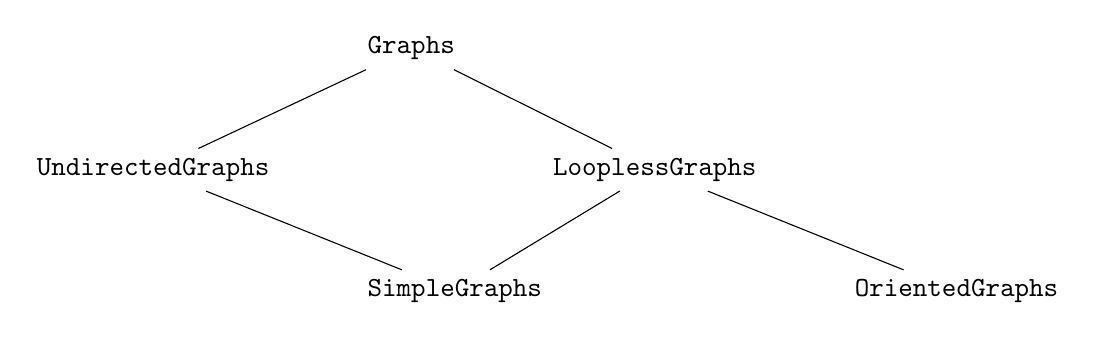
\begin{tikzpicture}[category/.style={font=\ttfamily}] \node (UG) [category]
{UndirectedGraphs}; \node (G) [category, above right=of UG] {Graphs}; \node
(SG) [category, below right=of UG] {SimpleGraphs}; \node (LG) [category, below
right=of G] {LooplessGraphs}; \node (OG) [category, below right=of LG]
{OrientedGraphs}; \draw (UG) -- (G) -- (LG) -- (OG); \draw (UG) -- (SG) --
(LG); \end{tikzpicture}  

This function is internally called by all graph constructing operations in \textsf{YAGS} to decide the graph category that the newly constructed graph is going to
belong. New graphs are always forced to comply with the \texttt{TargetGraphCategory}, so loops may be removed, and arrows may replaced by edges or viceversa,
depending on the category that the new graph belongs to. 

The \mbox{\texttt{\mdseries\slshape options stack}} is a mechanism provided by \textsf{GAP} to pass implicit parameters and is used by \texttt{TargetGraphCategory} so that the user may indicate the graph category she/he wants for the new
graph. 
\begin{Verbatim}[commandchars=!@|,fontsize=\small,frame=single,label=Example]
  !gapprompt@gap>| !gapinput@SetDefaultGraphCategory(SimpleGraphs);             |
  !gapprompt@gap>| !gapinput@g1:=CompleteGraph(2);                              |
  Graph( Category := SimpleGraphs, Order := 2, Size := 
  1, Adjacencies := [ [ 2 ], [ 1 ] ] )
  !gapprompt@gap>| !gapinput@g2:=CompleteGraph(2:GraphCategory:=OrientedGraphs);|
  Graph( Category := OrientedGraphs, Order := 2, Size := 
  1, Adjacencies := [ [ 2 ], [  ] ] )
  !gapprompt@gap>| !gapinput@DisjointUnion(g1,g2);|
  Graph( Category := LooplessGraphs, Order := 4, Size := 
  3, Adjacencies := [ [ 2 ], [ 1 ], [ 4 ], [  ] ] )
  !gapprompt@gap>| !gapinput@DisjointUnion(g1,g2:GraphCategory:=UndirectedGraphs);|
  Graph( Category := UndirectedGraphs, Order := 4, Size := 
  2, Adjacencies := [ [ 2 ], [ 1 ], [ 4 ], [ 3 ] ] )
\end{Verbatim}
 

In the previous examples, \texttt{TargetGraphCategory} was called internally exactly once for each new graph constructed with the
following parameters: 
\begin{Verbatim}[commandchars=!@|,fontsize=\small,frame=single,label=Example]
  !gapprompt@gap>| !gapinput@TargetGraphCategory();|
  <Category "SimpleGraphs">
  !gapprompt@gap>| !gapinput@TargetGraphCategory(:GraphCategory:=OrientedGraphs);|
  <Category "OrientedGraphs">
  !gapprompt@gap>| !gapinput@TargetGraphCategory([g1,g2]);                       |
  <Category "LooplessGraphs">
  !gapprompt@gap>| !gapinput@TargetGraphCategory([g1,g2]:GraphCategory:=UndirectedGraphs);|
  <Category "UndirectedGraphs">
\end{Verbatim}
 }

 

\subsection{\textcolor{Chapter }{Tetrahedron}}
\logpage{[ "B", 1, 163 ]}\nobreak
\hyperdef{L}{X7B44DDD485145773}{}
{\noindent\textcolor{FuncColor}{$\triangleright$\ \ \texttt{Tetrahedron\index{Tetrahedron@\texttt{Tetrahedron}}
\label{Tetrahedron}
}\hfill{\scriptsize (global variable)}}\\


 

The 1-skeleton of Plato's tetrahedron. 
\begin{Verbatim}[commandchars=!@|,fontsize=\small,frame=single,label=Example]
  !gapprompt@gap>| !gapinput@Tetrahedron;|
  Graph( Category := SimpleGraphs, Order := 4, Size := 
  6, Adjacencies := [ [ 2, 3, 4 ], [ 1, 3, 4 ], [ 1, 2, 4 ], 
    [ 1, 2, 3 ] ] )
\end{Verbatim}
 }

 

\subsection{\textcolor{Chapter }{TimeInSeconds}}
\logpage{[ "B", 1, 164 ]}\nobreak
\hyperdef{L}{X86C7A3E27AF64042}{}
{\noindent\textcolor{FuncColor}{$\triangleright$\ \ \texttt{TimeInSeconds({\mdseries\slshape })\index{TimeInSeconds@\texttt{TimeInSeconds}}
\label{TimeInSeconds}
}\hfill{\scriptsize (operation)}}\\


 

Returns the time in seconds since 1970-01-01 00:00:00 UTC as an integer. This
is useful to measure execution time. It can also be used to impose time
constraints on the execution of algorithms. Note however that the time
reported is the \emph{wall time}, not necessarily the time spent in the process you intend to measure. 
\begin{Verbatim}[commandchars=!@|,fontsize=\small,frame=single,label=Example]
  !gapprompt@gap>| !gapinput@TimeInSeconds();|
  1415551598
  !gapprompt@gap>| !gapinput@K:=CliqueGraph;;NumCli:=NumberOfCliques;;I:=Icosahedron;;|
  !gapprompt@gap>| !gapinput@t1:=TimeInSeconds();NumCli(K(K(K(K(I)))));TimeInSeconds()-t1;|
  1415551608
  44644
  103
\end{Verbatim}
 

Currently, this operation is not working on MS Windows. }

 

\subsection{\textcolor{Chapter }{TimesProduct}}
\logpage{[ "B", 1, 165 ]}\nobreak
\hyperdef{L}{X803A2BC67C63AA25}{}
{\noindent\textcolor{FuncColor}{$\triangleright$\ \ \texttt{TimesProduct({\mdseries\slshape G, H})\index{TimesProduct@\texttt{TimesProduct}}
\label{TimesProduct}
}\hfill{\scriptsize (operation)}}\\


 

Returns the times product of two graphs \mbox{\texttt{\mdseries\slshape G}} and \mbox{\texttt{\mdseries\slshape H}}, \mbox{\texttt{\mdseries\slshape G}} $\times$ \mbox{\texttt{\mdseries\slshape H}} (also known as the tensor product). 

The times product is computed as follows: 

For each pair of vertices $x \in G, y \in H$ we create a vertex $(x,y)$. Given two such vertices $(x,y)$ and $(x',y')$ they are adjacent iff $x \sim x'$ and $y \sim y'$. 
\begin{Verbatim}[commandchars=!@|,fontsize=\small,frame=single,label=Example]
  !gapprompt@gap>| !gapinput@g:=PathGraph(3);h:=CycleGraph(4);                              |
  Graph( Category := SimpleGraphs, Order := 3, Size := 
  2, Adjacencies := [ [ 2 ], [ 1, 3 ], [ 2 ] ] )
  Graph( Category := SimpleGraphs, Order := 4, Size := 
  4, Adjacencies := [ [ 2, 4 ], [ 1, 3 ], [ 2, 4 ], [ 1, 3 ] ] )
  !gapprompt@gap>| !gapinput@gh:=TimesProduct(g,h);         |
  Graph( Category := SimpleGraphs, Order := 12, Size := 
  16, Adjacencies := [ [ 6, 8 ], [ 5, 7 ], [ 6, 8 ], [ 5, 7 ], 
    [ 2, 4, 10, 12 ], [ 1, 3, 9, 11 ], [ 2, 4, 10, 12 ], 
    [ 1, 3, 9, 11 ], [ 6, 8 ], [ 5, 7 ], [ 6, 8 ], [ 5, 7 ] ] )
  !gapprompt@gap>| !gapinput@VertexNames(gh);                 |
  [ [ 1, 1 ], [ 1, 2 ], [ 1, 3 ], [ 1, 4 ], [ 2, 1 ], [ 2, 2 ], 
    [ 2, 3 ], [ 2, 4 ], [ 3, 1 ], [ 3, 2 ], [ 3, 3 ], [ 3, 4 ] ]
\end{Verbatim}
 }

 

\subsection{\textcolor{Chapter }{TorusGraph}}
\logpage{[ "B", 1, 166 ]}\nobreak
\hyperdef{L}{X87B9CA2A8552F40A}{}
{\noindent\textcolor{FuncColor}{$\triangleright$\ \ \texttt{TorusGraph({\mdseries\slshape n, m})\index{TorusGraph@\texttt{TorusGraph}}
\label{TorusGraph}
}\hfill{\scriptsize (function)}}\\


 

Returns (the underlying graph of) a triangulation of the torus on $n.m$ vertices. This graph is constructed using $\{1,2,\ldots, n\}\times\{1,2,\ldots, m\}$ as the vertex set; two of them being adjacent if their difference belongs to $\{(1,0),(0,1),(1,1)\}$ module ${\ensuremath{\mathbb Z}}_n\times{\ensuremath{\mathbb Z}}_m$. Hence, in the category of simple graphs, TorusGraph is a 6-regular graph
when $n,m\geq 3$. 
\begin{Verbatim}[commandchars=!@|,fontsize=\small,frame=single,label=Example]
  TorusGraph(4,4);
  Graph( Category := SimpleGraphs, Order := 16, Size := 48, Adjacencies := 
  [ [ 2, 4, 5, 6, 13, 16 ], [ 1, 3, 6, 7, 13, 14 ], [ 2, 4, 7, 8, 14, 15 ], 
    [ 1, 3, 5, 8, 15, 16 ], [ 1, 4, 6, 8, 9, 10 ], [ 1, 2, 5, 7, 10, 11 ], 
    [ 2, 3, 6, 8, 11, 12 ], [ 3, 4, 5, 7, 9, 12 ], [ 5, 8, 10, 12, 13, 14 ], 
    [ 5, 6, 9, 11, 14, 15 ], [ 6, 7, 10, 12, 15, 16 ], [ 7, 8, 9, 11, 13, 16 ], 
    [ 1, 2, 9, 12, 14, 16 ], [ 2, 3, 9, 10, 13, 15 ], [ 3, 4, 10, 11, 14, 16 ], 
    [ 1, 4, 11, 12, 13, 15 ] ] )
\end{Verbatim}
 

When $n,m\geq 4$, \texttt{TorusGraph( \mbox{\texttt{\mdseries\slshape n}}, \mbox{\texttt{\mdseries\slshape m}} )} is actually a Whitney triangulation: Every triangle of the graph is a face of
the triagulation. The clique behavior of these graphs were extensively studied
in \cite{LN99}. However, this operation constructs the described graph for all $n,m \geq 1$. 
\begin{Verbatim}[commandchars=!@|,fontsize=\small,frame=single,label=Example]
  !gapprompt@gap>| !gapinput@TorusGraph(2,4);|
  Graph( Category := SimpleGraphs, Order := 8, Size := 
  20, Adjacencies := [ [ 2, 4, 5, 6, 8 ], [ 1, 3, 5, 6, 7 ], 
    [ 2, 4, 6, 7, 8 ], [ 1, 3, 5, 7, 8 ], [ 1, 2, 4, 6, 8 ], 
    [ 1, 2, 3, 5, 7 ], [ 2, 3, 4, 6, 8 ], [ 1, 3, 4, 5, 7 ] ] )
  !gapprompt@gap>| !gapinput@TorusGraph(2,3);|
  Graph( Category := SimpleGraphs, Order := 6, Size := 
  15, Adjacencies := [ [ 2, 3, 4, 5, 6 ], [ 1, 3, 4, 5, 6 ], 
    [ 1, 2, 4, 5, 6 ], [ 1, 2, 3, 5, 6 ], [ 1, 2, 3, 4, 6 ], 
    [ 1, 2, 3, 4, 5 ] ] )
\end{Verbatim}
 

Note that in these cases, \texttt{TorusGraph( \mbox{\texttt{\mdseries\slshape n}}, \mbox{\texttt{\mdseries\slshape m}} )} is not 6-regular nor a Whitney triangulation. }

 

\subsection{\textcolor{Chapter }{TreeGraph}}
\logpage{[ "B", 1, 167 ]}\nobreak
\hyperdef{L}{X7C7EAB207C957EB1}{}
{\noindent\textcolor{FuncColor}{$\triangleright$\ \ \texttt{TreeGraph({\mdseries\slshape arity, depth})\index{TreeGraph@\texttt{TreeGraph}}
\label{TreeGraph}
}\hfill{\scriptsize (operation)}}\\
\noindent\textcolor{FuncColor}{$\triangleright$\ \ \texttt{TreeGraph({\mdseries\slshape ArityList})\index{TreeGraph@\texttt{TreeGraph}}
\label{TreeGraph}
}\hfill{\scriptsize (operation)}}\\


 

Returns a tree, a connected cycle-free graph. In its second form, the vertices
at height \mbox{\texttt{\mdseries\slshape k}} (the root vertex has height 1 here) have \texttt{ArityList[\mbox{\texttt{\mdseries\slshape k}}]} children. In its first form, all vertices, but the leaves, have \mbox{\texttt{\mdseries\slshape arity}} children and the height of the leaves is \mbox{\texttt{\mdseries\slshape depth}}+1. 
\begin{Verbatim}[commandchars=!@|,fontsize=\small,frame=single,label=Example]
  !gapprompt@gap>| !gapinput@TreeGraph(2,3);                                                  |
  Graph( Category := SimpleGraphs, Order := 15, Size := 
  14, Adjacencies := [ [ 2, 3 ], [ 1, 4, 5 ], [ 1, 6, 7 ], [ 2, 8, 9 ], 
    [ 2, 10, 11 ], [ 3, 12, 13 ], [ 3, 14, 15 ], [ 4 ], [ 4 ], [ 5 ], 
    [ 5 ], [ 6 ], [ 6 ], [ 7 ], [ 7 ] ] )
  !gapprompt@gap>| !gapinput@TreeGraph([3,2,2]);|
  Graph( Category := SimpleGraphs, Order := 22, Size := 
  21, Adjacencies := [ [ 2, 3, 4 ], [ 1, 5, 6 ], [ 1, 7, 8 ], 
    [ 1, 9, 10 ], [ 2, 11, 12 ], [ 2, 13, 14 ], [ 3, 15, 16 ], 
    [ 3, 17, 18 ], [ 4, 19, 20 ], [ 4, 21, 22 ], [ 5 ], [ 5 ], [ 6 ], 
    [ 6 ], [ 7 ], [ 7 ], [ 8 ], [ 8 ], [ 9 ], [ 9 ], [ 10 ], [ 10 ] ] )
\end{Verbatim}
 }

 

\subsection{\textcolor{Chapter }{TrivialGraph}}
\logpage{[ "B", 1, 168 ]}\nobreak
\hyperdef{L}{X82C1EADA7E3EE838}{}
{\noindent\textcolor{FuncColor}{$\triangleright$\ \ \texttt{TrivialGraph\index{TrivialGraph@\texttt{TrivialGraph}}
\label{TrivialGraph}
}\hfill{\scriptsize (global variable)}}\\


 

The one vertex graph. 
\begin{Verbatim}[commandchars=!@|,fontsize=\small,frame=single,label=Example]
  !gapprompt@gap>| !gapinput@TrivialGraph;|
  Graph( Category := SimpleGraphs, Order := 1, Size := 
  0, Adjacencies := [ [  ] ] )
\end{Verbatim}
 }

 

\subsection{\textcolor{Chapter }{UFFind}}
\logpage{[ "B", 1, 169 ]}\nobreak
\hyperdef{L}{X795BE08A79C126FC}{}
{\noindent\textcolor{FuncColor}{$\triangleright$\ \ \texttt{UFFind({\mdseries\slshape UFS, x})\index{UFFind@\texttt{UFFind}}
\label{UFFind}
}\hfill{\scriptsize (function)}}\\


 

For internal use. Implements the \mbox{\texttt{\mdseries\slshape find}} operation on the \mbox{\texttt{\mdseries\slshape union-find structure}}. }

 

\subsection{\textcolor{Chapter }{UFUnite}}
\logpage{[ "B", 1, 170 ]}\nobreak
\hyperdef{L}{X8105AD137ECF5AE4}{}
{\noindent\textcolor{FuncColor}{$\triangleright$\ \ \texttt{UFUnite({\mdseries\slshape UFS, x, y})\index{UFUnite@\texttt{UFUnite}}
\label{UFUnite}
}\hfill{\scriptsize (function)}}\\


 

For internal use. Implements the \mbox{\texttt{\mdseries\slshape unite}} operation on the \mbox{\texttt{\mdseries\slshape union-find structure}}. }

 

\subsection{\textcolor{Chapter }{UndirectedGraphs}}
\logpage{[ "B", 1, 171 ]}\nobreak
\hyperdef{L}{X7CC6D5C77C0CCFA3}{}
{\noindent\textcolor{FuncColor}{$\triangleright$\ \ \texttt{UndirectedGraphs({\mdseries\slshape G})\index{UndirectedGraphs@\texttt{UndirectedGraphs}}
\label{UndirectedGraphs}
}\hfill{\scriptsize (function)}}\\


 \texttt{UndirectedGraphs} is a graph category in \textsf{YAGS}. A graph in this category may contain edges and loops, but no arrows. The
parent of this category is \texttt{Graphs}. 
\begin{Verbatim}[commandchars=!@|,fontsize=\small,frame=single,label=Example]
  !gapprompt@gap>| !gapinput@GraphByWalks([1,1],[1,2],[2,1],[3,2]:GraphCategory:=Graphs);|
  Graph( Category := Graphs, Order := 3, Size := 4, Adjacencies := 
  [ [ 1, 2 ], [ 1 ], [ 2 ] ] )
  !gapprompt@gap>| !gapinput@GraphByWalks([1,1],[1,2],[2,1],[3,2]:GraphCategory:=UndirectedGraphs);|
  Graph( Category := UndirectedGraphs, Order := 3, Size := 
  3, Adjacencies := [ [ 1, 2 ], [ 1, 3 ], [ 2 ] ] )
\end{Verbatim}
 }

 

\subsection{\textcolor{Chapter }{UnitsRingGraph}}
\logpage{[ "B", 1, 172 ]}\nobreak
\hyperdef{L}{X7FDA5DD47D181699}{}
{\noindent\textcolor{FuncColor}{$\triangleright$\ \ \texttt{UnitsRingGraph({\mdseries\slshape Rng})\index{UnitsRingGraph@\texttt{UnitsRingGraph}}
\label{UnitsRingGraph}
}\hfill{\scriptsize (operation)}}\\


 

Returns the graph G whose vertices are the elements of \mbox{\texttt{\mdseries\slshape Rng}} such that x is adjacent to y iff x+z=y for some unit z of \mbox{\texttt{\mdseries\slshape Rng}}. 
\begin{Verbatim}[commandchars=!@|,fontsize=\small,frame=single,label=Example]
  !gapprompt@gap>| !gapinput@UnitsRingGraph(ZmodnZ(8));    |
  Graph( Category := SimpleGraphs, Order := 8, Size := 
  16, Adjacencies := [ [ 2, 4, 6, 8 ], [ 1, 3, 5, 7 ], [ 2, 4, 6, 8 ], 
    [ 1, 3, 5, 7 ], [ 2, 4, 6, 8 ], [ 1, 3, 5, 7 ], [ 2, 4, 6, 8 ], 
    [ 1, 3, 5, 7 ] ] )
\end{Verbatim}
 }

 

\subsection{\textcolor{Chapter }{VertexDegree}}
\logpage{[ "B", 1, 173 ]}\nobreak
\hyperdef{L}{X7B5898D98493A41D}{}
{\noindent\textcolor{FuncColor}{$\triangleright$\ \ \texttt{VertexDegree({\mdseries\slshape G, x})\index{VertexDegree@\texttt{VertexDegree}}
\label{VertexDegree}
}\hfill{\scriptsize (operation)}}\\


 

Returns the degree of vertex \mbox{\texttt{\mdseries\slshape x}} in Graph \mbox{\texttt{\mdseries\slshape G}}. 
\begin{Verbatim}[commandchars=!@|,fontsize=\small,frame=single,label=Example]
  !gapprompt@gap>| !gapinput@g:=PathGraph(3);|
  Graph( Category := SimpleGraphs, Order := 3, Size := 
  2, Adjacencies := [ [ 2 ], [ 1, 3 ], [ 2 ] ] )
  !gapprompt@gap>| !gapinput@VertexDegree(g,1);|
  1
  !gapprompt@gap>| !gapinput@VertexDegree(g,2);|
  2
\end{Verbatim}
 }

 

\subsection{\textcolor{Chapter }{VertexDegrees}}
\logpage{[ "B", 1, 174 ]}\nobreak
\hyperdef{L}{X8406A82E7973EC00}{}
{\noindent\textcolor{FuncColor}{$\triangleright$\ \ \texttt{VertexDegrees({\mdseries\slshape G})\index{VertexDegrees@\texttt{VertexDegrees}}
\label{VertexDegrees}
}\hfill{\scriptsize (operation)}}\\


 

Returns the list of degrees of the vertices in graph \mbox{\texttt{\mdseries\slshape G}}. 
\begin{Verbatim}[commandchars=!@|,fontsize=\small,frame=single,label=Example]
  !gapprompt@gap>| !gapinput@g:=GemGraph;|
  Graph( Category := SimpleGraphs, Order := 5, Size := 
  7, Adjacencies := [ [ 2, 3, 4, 5 ], [ 1, 3 ], [ 1, 2, 4 ], 
    [ 1, 3, 5 ], [ 1, 4 ] ] )
  !gapprompt@gap>| !gapinput@VertexDegrees(g);|
  [ 4, 2, 3, 3, 2 ]
\end{Verbatim}
 }

 

\subsection{\textcolor{Chapter }{VertexNames}}
\logpage{[ "B", 1, 175 ]}\nobreak
\hyperdef{L}{X86050933823255F1}{}
{\noindent\textcolor{FuncColor}{$\triangleright$\ \ \texttt{VertexNames({\mdseries\slshape G})\index{VertexNames@\texttt{VertexNames}}
\label{VertexNames}
}\hfill{\scriptsize (attribute)}}\\


 

Return the list of names of the vertices of \mbox{\texttt{\mdseries\slshape G}}. The vertices of a graph in \textsf{YAGS} are always $\{1,2, \ldots, Order(G)\}$, but depending on how the graph was constructed, its vertices may have also
some \mbox{\texttt{\mdseries\slshape names}}, that help us identify the origin of the vertices. \textsf{YAGS} will always try to store meaninful names for the vertices. For example, in the
case of the LineGraph, the vertex names of the new graph are the edges of the
old graph. 
\begin{Verbatim}[commandchars=!@|,fontsize=\small,frame=single,label=Example]
  !gapprompt@gap>| !gapinput@g:=LineGraph(DiamondGraph);          |
  Graph( Category := SimpleGraphs, Order := 5, Size := 
  8, Adjacencies := [ [ 2, 3, 4 ], [ 1, 3, 4, 5 ], [ 1, 2, 5 ], 
    [ 1, 2, 5 ], [ 2, 3, 4 ] ] )
  !gapprompt@gap>| !gapinput@VertexNames(g);|
  [ [ 1, 2 ], [ 1, 3 ], [ 1, 4 ], [ 2, 3 ], [ 3, 4 ] ]
  !gapprompt@gap>| !gapinput@Edges(DiamondGraph);|
  [ [ 1, 2 ], [ 1, 3 ], [ 1, 4 ], [ 2, 3 ], [ 3, 4 ] ]
\end{Verbatim}
 }

 

\subsection{\textcolor{Chapter }{Vertices}}
\logpage{[ "B", 1, 176 ]}\nobreak
\hyperdef{L}{X79E4BB4F849AC8A1}{}
{\noindent\textcolor{FuncColor}{$\triangleright$\ \ \texttt{Vertices({\mdseries\slshape G})\index{Vertices@\texttt{Vertices}}
\label{Vertices}
}\hfill{\scriptsize (operation)}}\\


 

Returns the list [1..Order( \mbox{\texttt{\mdseries\slshape G}} )]. 
\begin{Verbatim}[commandchars=!@|,fontsize=\small,frame=single,label=Example]
  !gapprompt@gap>| !gapinput@Vertices(Icosahedron);|
  [ 1 .. 12 ]
\end{Verbatim}
 }

 

\subsection{\textcolor{Chapter }{WheelGraph}}
\logpage{[ "B", 1, 177 ]}\nobreak
\hyperdef{L}{X817EA60D828A765E}{}
{\noindent\textcolor{FuncColor}{$\triangleright$\ \ \texttt{WheelGraph({\mdseries\slshape n})\index{WheelGraph@\texttt{WheelGraph}}
\label{WheelGraph}
}\hfill{\scriptsize (operation)}}\\
\noindent\textcolor{FuncColor}{$\triangleright$\ \ \texttt{WheelGraph({\mdseries\slshape n, r})\index{WheelGraph@\texttt{WheelGraph}}
\label{WheelGraph}
}\hfill{\scriptsize (operation)}}\\


 

In its first form \texttt{WheelGraph} returns the wheel graph on \mbox{\texttt{\mdseries\slshape n}}+1 vertices. This is the cone of a cycle: a central vertex adjacent to all the
vertices of an \mbox{\texttt{\mdseries\slshape n}}-cycle. 
\begin{Verbatim}[commandchars=!@|,fontsize=\small,frame=single,label=Example]
  !gapprompt@gap>| !gapinput@WheelGraph(5);|
  Graph( Category := SimpleGraphs, Order := 6, Size := 
  10, Adjacencies := [ [ 2, 3, 4, 5, 6 ], [ 1, 3, 6 ], [ 1, 2, 4 ], 
    [ 1, 3, 5 ], [ 1, 4, 6 ], [ 1, 2, 5 ] ] )
\end{Verbatim}
 

In its second form, \texttt{WheelGraph} returns returns the wheel graph, but adding \mbox{\texttt{\mdseries\slshape r}}-1 layers, each layer is a new \mbox{\texttt{\mdseries\slshape n}}-cycle joined to the previous layer by a zigzagging 2\mbox{\texttt{\mdseries\slshape n}}-cycle. This graph is a triangulation of the disk. 
\begin{Verbatim}[commandchars=!@|,fontsize=\small,frame=single,label=Example]
  !gapprompt@gap>| !gapinput@WheelGraph(5,2);|
  Graph( Category := SimpleGraphs, Order := 11, Size := 
  25, Adjacencies := [ [ 2, 3, 4, 5, 6 ], [ 1, 3, 6, 7, 8 ], 
    [ 1, 2, 4, 8, 9 ], [ 1, 3, 5, 9, 10 ], [ 1, 4, 6, 10, 11 ], 
    [ 1, 2, 5, 7, 11 ], [ 2, 6, 8, 11 ], [ 2, 3, 7, 9 ], 
    [ 3, 4, 8, 10 ], [ 4, 5, 9, 11 ], [ 5, 6, 7, 10 ] ] )
  !gapprompt@gap>| !gapinput@WheelGraph(5,3);|
  Graph( Category := SimpleGraphs, Order := 16, Size := 
  40, Adjacencies := [ [ 2, 3, 4, 5, 6 ], [ 1, 3, 6, 7, 8 ], 
    [ 1, 2, 4, 8, 9 ], [ 1, 3, 5, 9, 10 ], [ 1, 4, 6, 10, 11 ], 
    [ 1, 2, 5, 7, 11 ], [ 2, 6, 8, 11, 12, 13 ], [ 2, 3, 7, 9, 13, 14 ],
    [ 3, 4, 8, 10, 14, 15 ], [ 4, 5, 9, 11, 15, 16 ], 
    [ 5, 6, 7, 10, 12, 16 ], [ 7, 11, 13, 16 ], [ 7, 8, 12, 14 ], 
    [ 8, 9, 13, 15 ], [ 9, 10, 14, 16 ], [ 10, 11, 12, 15 ] ] )
\end{Verbatim}
 }

 

\subsection{\textcolor{Chapter }{YAGSExec}}
\logpage{[ "B", 1, 178 ]}\nobreak
\hyperdef{L}{X8150D2E37EA1F25D}{}
{\noindent\textcolor{FuncColor}{$\triangleright$\ \ \texttt{YAGSExec({\mdseries\slshape ProgName, InString})\index{YAGSExec@\texttt{YAGSExec}}
\label{YAGSExec}
}\hfill{\scriptsize (operation)}}\\


 

For internal use. Calls external program \mbox{\texttt{\mdseries\slshape ProgName}} located in directory \texttt{\mbox{\texttt{\mdseries\slshape YAGS-DIR}}/bin/} feeding it with \mbox{\texttt{\mdseries\slshape InString}} as input and returning the output of the external program as a string. \texttt{fail} is returned if the program could not be located. 
\begin{Verbatim}[commandchars=!@|,fontsize=\small,frame=single,label=Example]
  !gapprompt@gap>| !gapinput@YAGSExec("time","");|
  "1415551127\n"
  !gapprompt@gap>| !gapinput@YAGSExec("nauty","l=0$=1dacn=5 g1,2,3. xbzq");|
  "(4,5)\n(2,3)\n[2,3,4,5,1]\n[\"cb0c\",\"484f264\",\"b0e19f1\"]\n"
\end{Verbatim}
 

Currently, this operation is not working on MS Windows nor in Mac OS X. }

 

\subsection{\textcolor{Chapter }{YAGSInfo}}
\logpage{[ "B", 1, 179 ]}\nobreak
\hyperdef{L}{X865EB51A79C27268}{}
{\noindent\textcolor{FuncColor}{$\triangleright$\ \ \texttt{YAGSInfo\index{YAGSInfo@\texttt{YAGSInfo}}
\label{YAGSInfo}
}\hfill{\scriptsize (global variable)}}\\


 

A global record where much \textsf{YAGS}-related information is stored. This is intended for internal use, and much of
this information is undocumented, but some of the data stored here could
possibly be useful for advanced users. 

However, storing user information in this record and/or changing the values of
the stored information is discouraged and may produce unpredictable results
and an unstable system. 
\begin{Verbatim}[commandchars=!@|,fontsize=\small,frame=single,label=Example]
  !gapprompt@gap>| !gapinput@YAGSInfo;|
  rec( Arch := 1, AuxInfo := "/dev/null",
    DataDirectory := "/opt/gap4r7/pkg/yags/data",
    Directory := "/opt/gap4r7/pkg/yags",
    Draw :=
      rec( opts := [  ],
        prog := "/opt/gap4r7/pkg/yags/bin/draw/application.linux64/draw" ),
    Version := "0.0.1",
    graph6 := rec( BinListToNum := function( L ) ... end,
        BinListToNumList := function( L ) ... end,
        HararyList := [ [ 1, 0, 1 ], [ 2, 0, 1 ], [ 2, 1, 1 ],
            [ 3, 0, 1 ], [ 3, 1, 1 ], [ 3, 2, 1 ], [ 3, 3, 1 ],
            [ 4, 0, 1 ], [ 4, 1, 1 ], [ 4, 2, 1 ], [ 4, 3, 3 ],
            [ 4, 2, 2 ], [ 4, 3, 1 ], [ 4, 3, 2 ], [ 4, 4, 1 ],
  	  
     --- many more lines here ---
     
            [ 6, 13, 1 ], [ 6, 11, 7 ], [ 6, 11, 9 ], [ 6, 11, 8 ],
            [ 6, 12, 4 ], [ 6, 12, 5 ], [ 6, 13, 2 ], [ 6, 14, 1 ],
            [ 6, 15, 1 ] ], McKayN := function( n ) ... end,
        McKayR := function( L ) ... end,
        NumListToString := function( L ) ... end,
        NumToBinList := function( n ) ... end,
        PadLeftnSplitList6 := function( L ) ... end,
        PadRightnSplitList6 := function( L ) ... end,
        StringToBinList := function( Str ) ... end ) )
\end{Verbatim}
 }

 }

 }

\def\bibname{References\logpage{[ "Bib", 0, 0 ]}
\hyperdef{L}{X7A6F98FD85F02BFE}{}
}

\bibliographystyle{mapbib}
\bibliography{biblio}

\addcontentsline{toc}{chapter}{References}

\def\indexname{Index\logpage{[ "Ind", 0, 0 ]}
\hyperdef{L}{X83A0356F839C696F}{}
}

\cleardoublepage
\phantomsection
\addcontentsline{toc}{chapter}{Index}


\printindex

\newpage
\immediate\write\pagenrlog{["End"], \arabic{page}];}
\immediate\closeout\pagenrlog
\end{document}
